%%%%%%%%%%%%%%%%%%%%%%%%%%%%%%%%%%%%%%%%%%%%%%%%%%%%%%%%%%%%%%%%%%%%%%%%%%%%%%%
%                                                                             %
% Trabajo Terminal 2024-A053                                                  %
%                                                                             %
% Estimación de precios de mercado de departamentos en la Ciudad de México    %
%                                                                             %
% Alumno: Humberto Alejandro Ortega Alcocer                                   %
% Director: Mtro. Ariel López Rojas                                           %
%                                                                             %
% Escuela Superior de Cómputo                                                 %
% Instituto Politécnico Nacional                                              %
%                                                                             %
% 2023 - 2024                                                                 %
%%%%%%%%%%%%%%%%%%%%%%%%%%%%%%%%%%%%%%%%%%%%%%%%%%%%%%%%%%%%%%%%%%%%%%%%%%%%%%%

% Configuración del documento
% !TeX program = pdflatex
% !TeX encoding = UTF-8
% !TeX root = 2024-A053.tex
% !TeX spellcheck = es_MX

% Define el tipo de documento
\documentclass[12pt, a4paper, titlepage]{report} % Formato de reporte

% Importamos el preámbulo
%%%%%%%%%%%%%%%%%%%%%%%%%%%%%%%%%%%%%%%%%%%%%%%%%%%%%%%%%%%%%%%%%%%%%%%%%%%%%%%
%                                                                             %
% Preámbulo del documento                                                     %
%                                                                             %
%%%%%%%%%%%%%%%%%%%%%%%%%%%%%%%%%%%%%%%%%%%%%%%%%%%%%%%%%%%%%%%%%%%%%%%%%%%%%%%

% Paquetes para el idioma
\usepackage[spanish, es-lcroman]{babel}
\usepackage[utf8]{inputenc}
\usepackage[T1]{fontenc}

% Configuraciones para el párrafo
\usepackage{parskip}

% Paquetes para la tipografía
\usepackage[linesnumbered,lined,boxed,commentsnumbered]{algorithm2e}
\usepackage{enumitem,kantlipsum}

% Paquetes para usar fuentes de texto
\usepackage{array}
\usepackage{placeins}

% Apéndices
\usepackage[toc,page]{appendix}

% Tablas
\usepackage{tabularx}

% Paquetes para las referencias
\usepackage{float}
\usepackage{subfig}
\usepackage{comment}

% http://ctan.org/pkg/booktabs
\usepackage{booktabs}
\newcommand{\tabitem}{~~\llap{\textbullet}~~}

% Paquetes para las imágenes
\usepackage{graphicx}

% Color
\usepackage{color}
\usepackage{xcolor}
\usepackage{colortbl}

% Colores para el documento
\definecolor{guindapoli}{RGB}{102, 0, 51}
\definecolor{azulescom}{RGB}{0, 0, 102}
\definecolor{azulclaro}{RGB}{222, 232, 255}
\definecolor{azulfuerte}{RGB}{60, 150, 250}
\definecolor{blanco}{RGB}{255, 255, 255}

% Paquetes para las URL
\usepackage[hidelinks]{hyperref}

% Paquetes para las referencias
\usepackage{verbatim}

% Glosario
\usepackage[acronym]{glossaries}

%%Glosario
\usepackage{glossaries}

\usepackage{pdfpages}

% Códigos y codificación para caracteres en español
\usepackage{listings}

% Colores para código por defecto.
\definecolor{commentcolor}{RGB}{ 192, 192, 192 }
\definecolor{backcolour}{RGB}{ 249, 249, 249 }

% Estilo para código por defecto.
\lstdefinestyle{codeStyle}{
	backgroundcolor=\color{backcolour}, commentstyle=\color{commentcolor},
	keywordstyle=\color{guindapoli},
	numberstyle=\tiny\color{azulescom},
	stringstyle=\color{azulfuerte},
	basicstyle=\ttfamily\footnotesize,
	breakatwhitespace=false,
	breaklines=true,
	captionpos=b,
	keepspaces=true,
	numbers=left,
	numbersep=5pt,
	showspaces=false,
	showstringspaces=false,
	showtabs=true,
	tabsize=3
}

% Configuración para código por defecto, con caracteres en español.
\lstset{
  breaklines=true,
  %breakatwhitespace=true,
  %style=codeStyle,
  literate=
  {á}{{\'a}}1 {é}{{\'e}}1 {í}{{\'i}}1 {ó}{{\'o}}1 {ú}{{\'u}}1
  {Á}{{\'A}}1 {É}{{\'E}}1 {Í}{{\'I}}1 {Ó}{{\'O}}1 {Ú}{{\'U}}1
  {à}{{\`a}}1 {è}{{\`e}}1 {ì}{{\`i}}1 {ò}{{\`o}}1 {ù}{{\`u}}1
  {À}{{\`A}}1 {È}{{\`E}}1 {Ì}{{\`I}}1 {Ò}{{\`O}}1 {Ù}{{\`U}}1
  {ä}{{\"a}}1 {ë}{{\"e}}1 {ï}{{\"i}}1 {ö}{{\"o}}1 {ü}{{\"u}}1
  {Ä}{{\"A}}1 {Ë}{{\"E}}1 {Ï}{{\"I}}1 {Ö}{{\"O}}1 {Ü}{{\"U}}1
  {â}{{\^a}}1 {ê}{{\^e}}1 {î}{{\^i}}1 {ô}{{\^o}}1 {û}{{\^u}}1
  {Â}{{\^A}}1 {Ê}{{\^E}}1 {Î}{{\^I}}1 {Ô}{{\^O}}1 {Û}{{\^U}}1
  {ã}{{\~a}}1 {ẽ}{{\~e}}1 {ĩ}{{\~i}}1 {õ}{{\~o}}1 {ũ}{{\~u}}1
  {Ã}{{\~A}}1 {Ẽ}{{\~E}}1 {Ĩ}{{\~I}}1 {Õ}{{\~O}}1 {Ũ}{{\~U}}1
  {œ}{{\oe}}1 {Œ}{{\OE}}1 {æ}{{\ae}}1 {Æ}{{\AE}}1 {ß}{{\ss}}1
  {ű}{{\H{u}}}1 {Ű}{{\H{U}}}1 {ő}{{\H{o}}}1 {Ő}{{\H{O}}}1
  {ç}{{\c c}}1 {Ç}{{\c C}}1 {ø}{{\o}}1 {Ø}{{\O}}1 {å}{{\r a}}1 {Å}{{\r A}}1
  {€}{{\euro}}1 {£}{{\pounds}}1 {«}{{\guillemotleft}}1
  {»}{{\guillemotright}}1 {ñ}{{\~n}}1 {Ñ}{{\~N}}1 {¿}{{?`}}1 {¡}{{!`}}1
}

% Definición de lenguaje para JavaScript
\lstdefinelanguage{javascript}{
    keywords={break, case, catch, continue, debugger, default, delete, do, else, finally, for, function, if, in, instanceof, new, return, switch, this, throw, try, typeof, var, void, while, with, let, const},
    sensitive=true,
    morecomment=[l]{//},
    morecomment=[s]{/*}{*/},
    morestring=[b]',
    morestring=[b]",
    morestring=[b]`,
    identifierstyle=\color{black}\ttfamily,
    commentstyle=\color{ipython_cyan}\ttfamily,
    stringstyle=\color{ipython_red}\ttfamily,
    keepspaces=true,
    showspaces=false,
    showstringspaces=false,
    rulecolor=\color{ipython_frame},
    frame=single,
    frameround={t}{t}{t}{t},
    framexleftmargin=6mm,
    numbers=left,
    numberstyle=\tiny\color{halfgray},
    backgroundcolor=\color{ipython_bg},
    %extendedchars=true,
    basicstyle=\scriptsize,
    keywordstyle=\color{ipython_green}\ttfamily,
}

% Definición de lenguaje para Dockerfile
\lstdefinelanguage{dockerfile}{
  morekeywords={FROM, RUN, CMD, LABEL, MAINTAINER, EXPOSE, ENV, ADD, COPY, ENTRYPOINT, VOLUME, USER, WORKDIR, ARG, ONBUILD, STOPSIGNAL, HEALTHCHECK, SHELL},
  morecomment=[l]{\#},
  morestring=[b]"
  identifierstyle=\color{black}\ttfamily,
  commentstyle=\color{ipython_cyan}\ttfamily,
  stringstyle=\color{ipython_red}\ttfamily,
  keepspaces=true,
  showspaces=false,
  showstringspaces=false,
  rulecolor=\color{ipython_frame},
  frame=single,
  frameround={t}{t}{t}{t},
  framexleftmargin=6mm,
  numbers=left,
  numberstyle=\tiny\color{halfgray},
  backgroundcolor=\color{ipython_bg},
  %extendedchars=true,
  basicstyle=\scriptsize,
  keywordstyle=\color{ipython_green}\ttfamily,
}

% Configuración para código en JSON.
\lstdefinelanguage{json}{
    basicstyle=\normalfont\ttfamily,
    numbers=left,
    stepnumber=1,
    numbersep=8pt,
    showstringspaces=false,
    breaklines=true,
    frame=single,
    literate=
     *{0}{{{\color{azulfuerte}0}}}{1}
      {1}{{{\color{azulfuerte}1}}}{1}
      {2}{{{\color{azulfuerte}2}}}{1}
      {3}{{{\color{azulfuerte}3}}}{1}
      {4}{{{\color{azulfuerte}4}}}{1}
      {5}{{{\color{azulfuerte}5}}}{1}
      {6}{{{\color{azulfuerte}6}}}{1}
      {7}{{{\color{azulfuerte}7}}}{1}
      {8}{{{\color{azulfuerte}8}}}{1}
      {9}{{{\color{azulfuerte}9}}}{1}
      {:}{{{\color{azulfuerte}{:}}}}{1}
      {,}{{{\color{azulfuerte}{,}}}}{1}
      {\{}{{{\color{azulfuerte}{\{}}}}{1}
      {\}}{{{\color{azulfuerte}{\}}}}}{1}
      {[}{{{\color{azulfuerte}{[}}}}{1}
      {]}{{{\color{azulfuerte}{]}}}}{1},
    identifierstyle=\color{black}\ttfamily,
    commentstyle=\color{ipython_cyan}\ttfamily,
    stringstyle=\color{ipython_red}\ttfamily,
    keepspaces=true,
    showspaces=false,
    %showstringspaces=false,
    rulecolor=\color{ipython_frame},
    %frame=single,
    frameround={t}{t}{t}{t},
    framexleftmargin=6mm,
    %numbers=left,
    numberstyle=\tiny\color{halfgray},
    backgroundcolor=\color{ipython_bg},
    %extendedchars=true,
    basicstyle=\scriptsize,
    keywordstyle=\color{ipython_green}\ttfamily,
}

% Configuración para código en Bash.
\lstdefinelanguage{bash}{
  morekeywords={access,and,break,class,continue,def,del,elif,else,except,exec,finally,for,from,global,if,import,in,is,lambda,not,or,pass,print,raise,return,try,while},
  morekeywords=[2]{abs,all,any,basestring,bin,bool,bytearray,callable,chr,classmethod,cmp,compile,complex,delattr,dict,dir,divmod,enumerate,eval,execfile,file,filter,float,format,frozenset,getattr,globals,hasattr,hash,help,hex,id,input,int,isinstance,issubclass,iter,len,list,locals,long,map,max,memoryview,min,next,object,oct,open,ord,pow,property,range,raw_input,reduce,reload,repr,reversed,round,set,setattr,slice,sorted,staticmethod,str,sum,super,tuple,type,unichr,unicode,vars,xrange,zip,apply,buffer,coerce,intern},
  morekeywords=[3]{jq}
  sensitive=true,
  morecomment=[l]{\#},
  morestring=[b]',
  morestring=[b]",
  morestring=[s]{'''}{'''},
  morestring=[s]{"""}{"""},
  identifierstyle=\color{black}\ttfamily,
  commentstyle=\color{ipython_cyan}\ttfamily,
  stringstyle=\color{ipython_red}\ttfamily,
  keepspaces=true,
  showspaces=false,
  showstringspaces=false,
  rulecolor=\color{ipython_frame},
  frame=single,
  frameround={t}{t}{t}{t},
  framexleftmargin=6mm,
  numbers=left,
  numberstyle=\tiny\color{halfgray},
  backgroundcolor=\color{ipython_bg},
  %extendedchars=true,
  basicstyle=\scriptsize,
  keywordstyle=\color{ipython_green}\ttfamily,
}

% Configuración para código en Python.

% Colores para código en Python.
\definecolor{maroon}{cmyk}{0, 0.87, 0.68, 0.32}
\definecolor{halfgray}{gray}{0.55}
\definecolor{ipython_frame}{RGB}{207, 207, 207}
\definecolor{ipython_bg}{RGB}{247, 247, 247}
\definecolor{ipython_red}{RGB}{186, 33, 33}
\definecolor{ipython_green}{RGB}{0, 128, 0}
\definecolor{ipython_cyan}{RGB}{64, 128, 128}
\definecolor{ipython_purple}{RGB}{170, 34, 255}

% Definición de lenguaje para código en Python.
\lstdefinelanguage{python}{
	morekeywords={access,and,break,class,continue,def,del,elif,else,except,exec,finally,for,from,global,if,import,in,is,lambda,not,or,pass,print,raise,return,try,while},
	morekeywords=[2]{abs,all,any,basestring,bin,bool,bytearray,callable,chr,classmethod,cmp,compile,complex,delattr,dict,dir,divmod,enumerate,eval,execfile,file,filter,float,format,frozenset,getattr,globals,hasattr,hash,help,hex,id,input,int,isinstance,issubclass,iter,len,list,locals,long,map,max,memoryview,min,next,object,oct,open,ord,pow,property,range,raw_input,reduce,reload,repr,reversed,round,set,setattr,slice,sorted,staticmethod,str,sum,super,tuple,type,unichr,unicode,vars,xrange,zip,apply,buffer,coerce,intern},
	sensitive=true,
	morecomment=[l]\#,
	morestring=[b]',
	morestring=[b]",
	morestring=[s]{'''}{'''},
	morestring=[s]{"""}{"""},
	morestring=[s]{r'}{'},
	morestring=[s]{r"}{"},
	morestring=[s]{r'''}{'''},
	morestring=[s]{r"""}{"""},
	morestring=[s]{u'}{'},
	morestring=[s]{u"}{"},
	morestring=[s]{u'''}{'''},
	morestring=[s]{u"""}{"""},
	identifierstyle=\color{black}\ttfamily,
	commentstyle=\color{ipython_cyan}\ttfamily,
	stringstyle=\color{ipython_red}\ttfamily,
	keepspaces=true,
	showspaces=false,
	showstringspaces=false,
	rulecolor=\color{ipython_frame},
	frame=single,
	frameround={t}{t}{t}{t},
	framexleftmargin=6mm,
	numbers=left,
	numberstyle=\tiny\color{halfgray},
	backgroundcolor=\color{ipython_bg},
  extendedchars=true,
	basicstyle=\scriptsize,
	keywordstyle=\color{ipython_green}\ttfamily,
}

% Paquete para unidades
\usepackage{siunitx}



% Importamos el glosario
%%%%%%%%%%%%%%%%%%%%%%%%%%%%%%%%%%%%%%%%%%%%%%%%%%%%%%%%%%%%%%%%%%%%%%%%%%%%%%%
%                                                                             %
% Glosario de términos                                                        %
%                                                                             %
%%%%%%%%%%%%%%%%%%%%%%%%%%%%%%%%%%%%%%%%%%%%%%%%%%%%%%%%%%%%%%%%%%%%%%%%%%%%%%%

\makeglossaries
\newglossaryentry{inmueble}
{
  name={Inmueble},
  text={inmueble},
  description={Todos los intereses, beneficios, derechos y gravámenes inherentes a la propiedad de bienes raíces físicos, donde los bienes raíces son la tierra junto con todas las mejoras que están permanentemente adheridas a ella y todos los accesorios asociados a la misma \cite{pagourtzi2003}}
}
\newglossaryentry{valuacion}
{
  name={Valuación},
  text={valuación},
  description={Valuación es la acción o efecto de valuar, a su vez, significa valorar, entendido como el reconocimiento o apreciación del valor de algo \cite{salas2015modelo}}
}
\newglossaryentry{dataset}
{
  name={Dataset},
  text={dataset},
  description={Conjunto de datos que se utilizan para entrenar un modelo de aprendizaje automático \cite{ibm2023redneuronal}}
}


% Ya existían.
\newglossaryentry{Convolucional}
{
	name={Convolucional},
	text={convolucional},
	description={Es un operador matemático el cual transforma dos funciones en una tercera función.\cite{refRAE}}
}
\newglossaryentry{Recurrente}{
	name={Recurrente},
	text={recurrente},
	description={Algo que vuelve a ocurrir o a aparecer después de un intervalo.\cite{refRAE}}
}
\newglossaryentry{Reconocimiento}{
	name={Reconocimiento},
	text={reconocimiento},
	description={Examinar algo o a alguien para así poder conocer su identidad, estado, naturaleza y circunstancias. Distinguir o identificar a una persona o una cosa entre varas por una serie de características.\cite{refOxfordLex}}
}
\newglossaryentry{Aprende}{
	name={Aprende},
	text={aprende},
	description={Adquirir el conocimiento de algo por medio del estudio, análisis o de la experiencia.\cite{refRAE}}
}
\newglossaryentry{Sistema}{
	name={Sistema},
	text={sistema},
    description={Conjunto de elementos con relaciones de interacción e interdependencia las cuales le confieren entidad propia al formar un todo unificado.\cite{refSistema}}
}
\newglossaryentry{Estado}{
	name={Estado},
	text={estado},
    description={Situación en que se encuentra alguien o algo, y en especial cada uno de sus sucesivos modos de ser o estar.\cite{refRAE}}
}
\newglossaryentry{Armonia}{
	name={Armonía},
	text={armonía},
    description={Unión y combinación de sonidos simultáneos y diferentes, pero acordes.\cite{refRAE}}
}
\newglossaryentry{Melodia}{
	name={Melodía},
	text={melodía},
    description={Es una sucesión lineal ordenada y coherente de sonidos musicales los cuales forman una unidad estructurada con un sentido musical, independiente del acompañamiento. \\Sucesión de sonidos que por su manera de combinarse resulta agradable de oír.\cite{refOxfordLex}}
}
\newglossaryentry{Estrofa}{
	name={Estrofa},
	text={estrofa},
    description={Conjunto de versos que generalmente se ajustan a una medida y a un ritmo determinado y constante.\cite{refRAE}}
}
\newglossaryentry{Acordes}{
	name={Acordes},
	text={acordes},
    description={Conjunto de notas musicales sonando al mismo tiempo.\cite{refRAE}}
}
\newglossaryentry{Estocastico}{
	name={Estocástico},
	text={estocástico},
    description={Que está sometido al azar y que es un objeto de análisis estadístico.\cite{refRAE}}
}
\newglossaryentry{Maquinas de Estados Finitos}{
	name={Máquinas de Estados Finitos},
	text={máquinas de estados finitos},
    description={Conocidas también como Finite State Machines por su traducción en inglés, nos sirven para realizar procesos bien definidos en un tiempo discreto. Reciben una entrada, realizan un proceso y nos entregan una salida.\cite{refMaquinasFinitas}}
}


% Importamos los acrónimos
%%%%%%%%%%%%%%%%%%%%%%%%%%%%%%%%%%%%%%%%%%%%%%%%%%%%%%%%%%%%%%%%%%%%%%%%%%%%%%%
%                                                                             %
% Acrónimos                                                                   %
%                                                                             %
%%%%%%%%%%%%%%%%%%%%%%%%%%%%%%%%%%%%%%%%%%%%%%%%%%%%%%%%%%%%%%%%%%%%%%%%%%%%%%%

% Valuación, economía, finanzas
\newacronym{deps}{DEPS}{Density Estimation and Profit Simulation}

% Instituciones
\newacronym{indaabin}{INDAABIN}{Instituto de Administración y Avalúos de Bienes Nacionales}
\newacronym{ivsc}{IVSC}{International Valuation Standards Council}
\newacronym{shn}{SHN}{Sociedad Hipotecaria Nacional}
\newacronym{cnbv}{CNBV}{Comisión Nacional Bancaria y de Valores}
\newacronym{sedeco}{SEDECO}{Secretaría de Desarrollo Económico}
\newacronym{bid}{BID}{Banco Interamericano de Desarrollo}

% Leyes
\newacronym{lfpdppp}{LFPDPPP}{Ley Federal de Protección de Datos Personales en Posesión de los Particulares}

% Tecnologías
\newacronym{ia}{IA}{Inteligencia Artificial}
\newacronym{arima}{ARIMA}{Modelo Autoregresivo de Media Móvil}
\newacronym{avm}{AVM}{Modelo de Valuación Automatica}
\newacronym{rna}{RNA}{Redes Neuronales Artificiales}
\newacronym{csv}{CSV}{Comma Separated Values (Valores Separados por Comas)}
\newacronym{mime}{MIME}{Multipurpose Internet Mail Extensions}
%
\newacronym{mvc}{MVC}{Modelo-Vista-Controlador}
\newacronym{orm}{ORM}{Object Relational Manager}
\newacronym{wsgi}{WSGI}{Web Server Gateway Interface}
\newacronym{dbms}{DBMS}{Sistema de gestión de base de datos}
\newacronym{bert}{BERT}{Bidirectional Encoder Representations from Transformers}
\newacronym{pln}{PLN}{Procesamiento del Lenguaje Natural}
\newacronym{mlm}{MLM}{Modelado de Lenguaje Enmascarado}
\newacronym{gpt}{GPT}{Generative Pretrained Transformer}
\newacronym{bpe}{BPE}{Byte Pair Encoding}
\newacronym{wip}{WIP}{Work In Progress}
\newacronym{cls}{CLS}{Classification}
\newacronym{sep}{SEP}{Separate}
\newacronym{json}{JSON}{Javascript Object Notation}
\newacronym{url}{URL}{Uniform Source Locator}
\newacronym{http}{HTTP}{Hypertext Transfer Protocol}
\newacronym{tcp}{TCP}{Transmission Control Protocol}
\newacronym{udp}{UDP}{User Datagram Protocol}
\newacronym{imap}{IMAP}{Internet Message Access Protocol}
\newacronym{pop}{POP}{Post Office Protocol}
\newacronym{smtp}{SMTP}{Simple Mail Transfer Protocol}
\newacronym{vps}{VPS}{Virtual Private Server}
\newacronym{ssl}{SSL}{Secure Socket Layer}
\newacronym{fqdn}{FQDN}{Fully Qualified Domain Name}
\newacronym{aws}{AWS}{Amazon Web Services}
\newacronym{gpu}{GPU}{Graphic Processor Unit}
\newacronym{ec2}{EC2}{Elastic Compute Cloud}
\newacronym{ui}{UI}{User Interface}
\newacronym{api}{API}{Application Programm Interface}
\newacronym{gcp}{GCP}{Google Cloud Platform}
\newacronym{sdk}{SDK}{Software Development Kit}
\newacronym{html}{HTML}{Hypertext Markup Language}
\newacronym{css}{CSS}{Cascading Style Sheet}
\newacronym{ecma}{ECMA}{European Computer Manufacturers Association}
\newacronym{https}{HTTPS}{Hypertext Transfer Protocol Secure}
\newacronym{tls}{TLS}{Transport Layer Security}
\newacronym{sql}{SQL}{Structured Query Language}
\newacronym{cad}{CAD}{Computer Aided Design}
\newacronym{cli}{CLI}{Command Line Interface}
\newacronym{s3}{S3}{Simple Storage Service}
\newacronym{hdd}{HDD}{Hard Drive Disk}
\newacronym{ssd}{SSD}{Solid State Drive}
\newacronym{iso}{ISO}{International Standardization Organization}
\newacronym{xml}{XML}{Extensible Markup Language}
\newacronym{svg}{SVG}{Scalable Vector Graphics}
\newacronym{rnn}{RNN}{Recurrent Neural Network}
\newacronym{lstm}{LSTM}{Long Short Term Memory}



%%%%%%%%%%%%%%%%%%%%%%%%%%%%%%%%%%%%%%%%%%%%%%%%%%%%%%%%%%%%%%%%%%%%%%%%%%%%%%%
%                                                                             %
% Inicio del documento                                                        %
%                                                                             %
%%%%%%%%%%%%%%%%%%%%%%%%%%%%%%%%%%%%%%%%%%%%%%%%%%%%%%%%%%%%%%%%%%%%%%%%%%%%%%%
\begin{document}

%%%%%%%%%%%%%%%%%%%%%%%%%%%%%%%%%%%%%%%%%%%%%%%%%%%%%%%%%%%%%%%%%%%%%%%%%%%%%%%
%                                                                             %
% Portada                                                                     %
%                                                                             %
%%%%%%%%%%%%%%%%%%%%%%%%%%%%%%%%%%%%%%%%%%%%%%%%%%%%%%%%%%%%%%%%%%%%%%%%%%%%%%%
\begin{titlepage}
  \newcommand{\HRule}{\rule{\linewidth}{0.5mm}}
  \begin{minipage}{0.48\textwidth}
    \begin{flushleft}
      \includegraphics[scale = 0.10]{imagenes/logotipos/escom.png}
    \end{flushleft}\end{minipage}
    \begin{minipage}{0.48\textwidth} \begin{flushright}
      \includegraphics[scale = 0.55]{imagenes/logotipos/ipn.png}
    \end{flushright}
  \end{minipage}
  \vspace*{.25cm}
  \begin{center}
    \begin{LARGE}
      \textcolor{guindapoli}{Instituto Politécnico Nacional}\\
    \end{LARGE}
    \vspace*{0.2in}
    \begin{Large}
      \textcolor{azulescom}{Escuela Superior de Cómputo}\\
    \end{Large}
    \vspace*{0.4in}
    \begin{large}
      Trabajo Terminal
    \end{large}

    \vspace*{0.2in}

    \begin{Large}
      \textbf{Plataforma web para la estimación de precios de mercado de departamentos en la Ciudad de México}\\
    \end{Large}
    \vspace*{0.2in}
    \begin{large}
      No. 2024-A053\\
    \end{large}
    \vspace*{0.2in}
    \rule{80mm}{.1mm}\\
    \vspace*{0.1in}
    \begin{large}
      \begin{center}
        \textbf{Presenta}:\\
        Humberto Alejandro Ortega Alcocer\\
      \end{center}
    \end{large}
    \begin{large}
      \textbf{Director}:\\
      Ariel López Rojas\\
    \end{large}
  \end{center}
\end{titlepage}

%%%%%%%%%%%%%%%%%%%%%%%%%%%%%%%%%%%%%%%%%%%%%%%%%%%%%%%%%%%%%%%%%%%%%%%%%%%%%%%
%                                                                             %
% Firmas de Directores                                                        %
%                                                                             %
%%%%%%%%%%%%%%%%%%%%%%%%%%%%%%%%%%%%%%%%%%%%%%%%%%%%%%%%%%%%%%%%%%%%%%%%%%%%%%%
  \newpage
  \section*{\textcolor{azulescom}{Firma de Director}}
  \vfill
  \noindent
  \parbox[b]{0.4\linewidth}{
    \strut
    Firmado por: \\[3cm]
    \hrule
    \vspace*{0.1in}
    Ariel López Rojas}
  \hfill
  \vfill
  \newpage

%%%%%%%%%%%%%%%%%%%%%%%%%%%%%%%%%%%%%%%%%%%%%%%%%%%%%%%%%%%%%%%%%%%%%%%%%%%%%%%
%                                                                             %
% Agradecimientos                                                             %
%                                                                             %
%%%%%%%%%%%%%%%%%%%%%%%%%%%%%%%%%%%%%%%%%%%%%%%%%%%%%%%%%%%%%%%%%%%%%%%%%%%%%%%
\section*{\textcolor{azulescom}{Agradecimientos}}
%\addcontentsline{toc}{section}{Agradecimientos}

{\setlength{\parindent}{15pt}
\indent En primer lugar, agradezco al Instituto Politécnico Nacional (IPN) y a
la Escuela Superior de Cómputo (ESCOM) por brindarme la oportunidad y los
recursos necesarios para formarme como profesional y llevar a cabo este proyecto.}

Quiero expresar mi más profundo agradecimiento a mi director de trabajo terminal,
Ariel López Rojas, por su invaluable apoyo, orientación y paciencia a lo largo
de este proyecto. Su experiencia y dedicación han sido fundamentales para la
culminación de este trabajo.

A mi familia, les agradezco desde el fondo de mi corazón por su amor
incondicional y por estar siempre a mi lado, brindándome la fuerza y el ánimo
necesarios en cada etapa de mi vida académica. En particular, quiero mencionar
con especial cariño a mi madre, Lourdes, quien ha sido mi principal
fuente de inspiración y motivación. A mis abuelos, Lourdes y Alejandro, cuyo
sabio consejo y apoyo constante me han guiado siempre. A mi hermano, Gerardo,
por su comprensión y respaldo incondicional.

A Maura, cuya comprensión y afecto han sido fundamentales para llegar
hasta aquí. Su amor y apoyo han sido una fuente constante de fortaleza.

A mis amigos, gracias por su inquebrantable apoyo moral y por
creer en mí incluso en los momentos más difíciles. Su compañía y aliento han
sido esenciales para llegar hasta aquí.

Este logro es también de ustedes. Gracias a todos.

\vspace{1cm}

\begin{flushright}
\textbf{Humberto Alejandro Ortega Alcocer}
\end{flushright}

\newpage

%%%%%%%%%%%%%%%%%%%%%%%%%%%%%%%%%%%%%%%%%%%%%%%%%%%%%%%%%%%%%%%%%%%%%%%%%%%%%%%
%                                                                             %
% Índice                                                                      %
%                                                                             %
%%%%%%%%%%%%%%%%%%%%%%%%%%%%%%%%%%%%%%%%%%%%%%%%%%%%%%%%%%%%%%%%%%%%%%%%%%%%%%%
  % Cambiar nombre de Apéndice a Índice
  \renewcommand\appendixpagename{Índice}
  \renewcommand\appendixtocname{Índice}

  \appendixpageoff

  \begin{appendices}
    \renewcommand*\contentsname{{\textcolor{azulescom}{Índice.}}}
    \tableofcontents
    \newpage

    % Índice de figuras
    \renewcommand*\listfigurename{{\textcolor{azulescom}{Índice de figuras.}}}
    \listoffigures
    \newpage

    % Índice de tablas
    \newpage
    \renewcommand*\listtablename{{\textcolor{azulescom}{Índice de cuadros.}}}
    \listoftables

  \end{appendices}
  \newpage

%%%%%%%%%%%%%%%%%%%%%%%%%%%%%%%%%%%%%%%%%%%%%%%%%%%%%%%%%%%%%%%%%%%%%%%%%%%%%%%
%                                                                             %
% Secciones del documento                                                     %
%                                                                             %
%%%%%%%%%%%%%%%%%%%%%%%%%%%%%%%%%%%%%%%%%%%%%%%%%%%%%%%%%%%%%%%%%%%%%%%%%%%%%%%
  %%%%%%%%%%%%%%%%%%%%%%%%%%%%%%%%%%%%%%%%%%%%%%%%%%%%%%%%%%%%%%%%%%%%%%%%%%%%%%%
%                                                                             %
% 01 - Introducción y objetivos                                               %
%                                                                             %
%%%%%%%%%%%%%%%%%%%%%%%%%%%%%%%%%%%%%%%%%%%%%%%%%%%%%%%%%%%%%%%%%%%%%%%%%%%%%%%

\chapter{\textcolor{azulescom}{Introducción}}

La industria inmobiliaria en la actualidad enfrenta grandes desafíos en la
valuación de bienes inmuebles, donde la precisión y la eficiencia son cruciales
para el éxito de las transacciones \cite{pagourtzi2003}. Los profesionales
del sector y los inversionistas a menudo encuentran dificultades para determinar
los precios más apropiados de cada inmueble debido a la falta de herramientas
eficientes y la complejidad del mercado inmobiliario \cite{nedovic2000}.
La propuesta de este trabajo terminal implica el uso de nuevas tecnologías que
le ofrezcan al usuario la posibilidad de obtener un precio de mercado.

La inteligencia artificial ha demostrado un gran potencial en el análisis y la
toma de decisiones en diversos campos de alto impacto en nuestra sociedad como
lo son la medicina, la construcción, las finanzas, el comercio electrónico y el
sector inmobiliario \cite{pagourtzi2003}. Algunas investigaciones han
propuesto el uso de técnicas de inteligencia artificial, como el aprendizaje
automático y las redes neuronales, para mejorar la cobertura geográfica en la
estimación de valores de propiedades \cite{worzala1995,limsombunchai2004}.
La valuación de bienes inmuebles requiere la consideración de múltiples factores,
como la ubicación, las características de la propiedad, las tendencias del mercado
y las condiciones económicas \cite{limsombunchai2004}. Estos factores hacen que la
valuación de propiedades sea una tarea compleja y desafiante, que podría beneficiarse
del uso de técnicas avanzadas de inteligencia artificial para analizar la información
y generar estimaciones precisas.

En este contexto, se han comparado múltiples algoritmos y metodologías de
aprendizaje automático, cómo Extra Trees (ET), k–Nearest Neighbors (KNN), y
Random Forest (RF), dónde se observa que cada mercado cuenta con características
específicas que requieren incluirse en el proceso de estimación y por lo tanto
deben considerarse para lograr mejores resultados \cite{choy2023}.
Sin embargo, el planteamiento fundamental puede ser adaptado fácilmente en función
de la cobertura geográfica deseada.

La propuesta del presente Trabajo Terminal se enfoca en el desarrollo de un
método de estimación de costo para departamentos que, mediante el uso de
Inteligencia Artificial, sea capaz de realizar estimaciones de costo útiles
para un precio de mercado en la Ciudad de México a manera de facilitar y
optimizar el tiempo que toma obtener un vistazo inicial a lo que podría ser el
valor del inmueble en cuestión.

Actualmente, en el mercado se encuentran algunas soluciones que hacen uso de
inteligencia artificial para la valuación de propiedades,
como Zillow's Zestimate \cite{zillow2023} y HouseCanary \cite{housecanary2021}.
Sin embargo, estas soluciones aún presentan limitaciones en términos de cobertura
y adaptabilidad a diferentes
mercados y contextos. La propuesta busca abordar estas limitaciones y ofrecer
una herramienta más adaptable al mercado mexicano, más específicamente al de la
Ciudad de México.

\section{Estado del Arte}
A continuación, se presenta el Cuadro \ref{table:PropuestasSimilares} con las
características de aplicaciones web similares y comparándolos con la propuesta.
Dentro de las características se incluye el tipo de aplicación, las características
de estimación de costo, la cobertura geográfica y el precio en el mercado.

\begin{table}[H]
    \caption[Resumen de productos similares]{Resumen de productos similares comparados con la propuesta}
    \centering
    \begin{tabular}{|m{3.5cm}|m{6.5cm}|m{3.5cm}|}
        \hline
          \rowcolor{azulclaro}
          \multicolumn{1}{|c|}{\textbf{Software}} &
          \multicolumn{1}{c|}{\textbf{Características}} &
          \multicolumn{1}{c|}{\textbf{Precio en el mercado}} \\
        \hline
        Zillow’s Zestimate \cite{zillow2023} & Aplicación web que ofrece una estimación de costo de bienes inmobiliarios, hace uso de inteligencia artificial para obtener los valores de cada característica, los datos usados son los propios de Zillow (marketplace de bienes raíces) permite ingresar detalles específicos a cada tipo de inmueble y ofrece una valuación muy precisa y detallada, sin embargo solo tiene cobertura en el mercado de EE.UU. y Canadá. & Gratuito \\
        \hline
        House Canary \cite{housecanary2021} & Aplicación web que ofrece una estimación de costo de bienes inmobiliarios, hace uso de inteligencia artificial para obtener las estimaciones de cada característica, permite ingresar detalles específicos a cada inmueble, sólo tiene cobertura en EE.UU. y Canadá. & Considerando el producto \textit{Agile Evaluation}, \$ 0.80 USD por valuación  \\
        \hline
        Estimador de costo de Inmuebles24 \cite{inmuebles24} & Aplicación web que ofrece una estimación aproximada de costo para bienes raíces, hace uso de inteligencia artificial para obtener la estimación de costo general, los datos utilizados son de su propio sitio web (marketplace de bienes raíces), su cobertura es baja y únicamente entrega el precio de mercado. & Gratuito \\
        \hline
        Propuesta de herramienta en el presente trabajo terminal & Aplicación web que ofrecerá una estimación aproximada de costo para departamentos en la Ciudad de México, hace uso de inteligencia artificial para obtener la estimación de costo general, la cobertura será determinada por la disponibilidad del conjunto de datos a emplear. & Gratuito \\
        \hline
    \end{tabular}
    \label{table:PropuestasSimilares}
\end{table}

\section{Objetivos}

\subsection{Objetivo general}

Crear una herramienta de apoyo para profesionales del sector inmobiliario,
inversionistas o cualquier persona interesada en la estimación de costo de algún
departamento en la Ciudad de México para que puedan obtener un precio de mercado.

Mediante el uso de un conjunto de datos (\gls{dataset}) y servicios de la nube (Amazon
Web Services) los datos se procesarán a fin de crear un módulo que pueda identificar
patrones a través de redes neuronales para ofrecer un estimado de precio a partir
de un conjunto de características que clasifiquen al inmueble. A su vez, se
desarrollará una interfaz web intuitiva a modo de prototipo con el fin de que el
usuario pueda visualizar el estimado de precio del inmueble en cuestión.

Dicha herramienta pretende ayudar a los usuarios descritos con el fin de que
puedan obtener una estimación de costo que les permita tener un aproximado de
precio de mercado.

\subsection{Objetivos particulares}

\begin{itemize}
  \item Generar un conjunto de datos (\gls{dataset}) con precios históricos de bienes
  inmobiliarios en la Ciudad de México para efecto de entrenamiento del modelo
  de aprendizaje automático.
  \item Hacer uso de alguna herramienta que utilice aprendizaje automático
  (machine learning) e implementar su uso en la nube para ayudar a procesar los
  anuncios de un tipo de inmueble particular.
  \item Desarrollar una interfaz web intuitiva a modo de prototipo que utilice
  una aplicación web alojada en infraestructura de nube para la captura de los
  datos del usuario así como la entrega de la estimación de precio calculada
  por el modelo.
\end{itemize}

\section{Justificación}

La generación de estimaciones precisas y eficientes para la valuación de bienes
inmuebles puede ser un desafío abrumador para profesionales y aficionados, debido
a la falta de herramientas adecuadas y la complejidad del mercado inmobiliario.
En ocasiones, se pueden recurrir a servicios especializados en la valuación de
propiedades, pero estos pueden resultar costosos y no siempre cumplir con las
expectativas del usuario. Por tanto, este trabajo terminal busca desarrollar una
herramienta que facilite el proceso de estimación de costos para departamentos
en la Ciudad de México, beneficiando a profesionales del sector inmobiliario,
inversionistas e interesados en general en el sector inmobiliario.

Por lo general, la valuación de bienes inmuebles implica la consideración de
múltiples factores, como la ubicación, las características de la propiedad y
las tendencias del mercado \cite{limsombunchai2004}. Estos patrones pueden ser
identificados mediante el uso de inteligencia artificial y el análisis de datos
históricos y actuales del mercado inmobiliario. Al enfocar el análisis en el
mercado de la Ciudad de México, se espera que el modelo propuesto sea más
relevante y preciso para este contexto específico.

El trabajo terminal propone utilizar técnicas avanzadas de inteligencia artificial,
como el aprendizaje automático y las redes neuronales, para mejorar la cobertura
en la estimación de costos de departamentos en la Ciudad de México \cite{worzala1995}.
Además, se plantea implementar la solución en un entorno en la nube, lo que
facilitaría la adaptación y flexibilidad de la plataforma, permitiendo su
actualización y mantenimiento independientemente de la implementación.

A diferencia de las soluciones existentes en el mercado, como Zillow's Zestimate
y HouseCanary, este proyecto busca desarrollar un método de estimación de costo
específicamente adaptado al mercado inmobiliario de la Ciudad de México, utilizando
tecnologías y enfoques diferentes para lograr resultados más precisos y relevantes
\cite{housecanary2021,zillow2023}.

Se utilizarán conocimientos adquiridos durante la carrera para llevar a cabo un
análisis eficaz y detallado de la problemática y las opciones de solución. Para
ello, se retomarán técnicas de gestión y diseño de proyectos vistas en
\textit{Administración de Proyectos}, \textit{Gestión Empresarial} e
\textit{Ingeniería de Software}, conocimientos de programación como en
\textit{Programación Orientada a Objetos}, \textit{Sistemas Distribuídos} y
\textit{Desarrollo Web}, técnicas de \textit{Inteligencia Artificial} y
\textit{Análisis de Datos} y, finalmente, se hará uso de herramientas de
comunicación y redacción científica vistas en \textit{Comunicación Oral y Escrita}
para un análisis detallado del ámbito de la valuación inmobiliaria permitiendo un
detallado y eficaz análisis del problema y las soluciones disponibles.

\section{Metodología}

Para el desarrollo de este trabajo terminal se optó por la metodología ágil SCRUM,
debido a que, como proceso de gestión de proyectos, se reduce complejidad y
permite actuar rápidamente ante cualquier cambio para poder satisfacer las
necesidades de los clientes. Una de las cualidades más importantes de SCRUM
es que nos ofrece una clara visibilidad sobre el avance del proyecto así como de
los pasos intermedios a realizar en cada sprint para alcanzar los objetivos. Además,
permite trabajar de manera eficiente colaborativamente, es decir, en equipo,
para obtener el mejor resultado posible.

Ken Schwaber y Jeff Sutherland \cite{schwaber2016} explican Scrum de una manera clara y simple.
Dicen que no es una colección de partes y/o componentes definidos de manera
prescriptiva, sino que está basado en un modelo de proceso empírico, basado en
la autoorganización de los equipos los cuales logran lidiar con lo imprevisible,
resolviendo los problemas complejos inspeccionándolos y adaptándose continuamente.

SCRUM contiene los siguientes eventos:

\begin{itemize}
  \item \textbf{Sprint Planning}: Reunión de planificación del sprint, en la que
  el equipo de desarrollo selecciona las tareas que se van a realizar durante el
  sprint.
  \item \textbf{Daily Scrum}: Reunión diaria de seguimiento, en la que el equipo
  de desarrollo se sincroniza sobre el estado de las tareas.
  \item \textbf{Sprint Review}: Reunión de revisión del sprint, en la que el
  equipo de desarrollo muestra los resultados del sprint.
  \item \textbf{Sprint Retrospective}: Reunión de retrospectiva del sprint, en
  la que el equipo de desarrollo analiza el sprint y propone mejoras.
\end{itemize}

Estos eventos existen con el fin de establecer una regularidad y minimizar la
necesidad de reuniones no definidas en Scrum. Estos eventos son bloques de
tiempo (\textit{time boxes}), de tal forma que todos cuentan con una duración máxima.

También se definen los siguientes artefactos:

\begin{itemize}
  \item \textbf{Product Backlog}: Lista de requisitos del producto, ordenados
  por prioridad.
  \item \textbf{Sprint Backlog}: Lista de requisitos del producto seleccionados
  para el sprint actual.
  \item \textbf{Incremento}: Conjunto de requisitos del producto completados
  durante el sprint actual.
\end{itemize}

Los artefactos en SCRUM se definen para así fomentar la transparencia de la
información de tal manera que todos los involucrados tengan el mismo entendimiento
de que es lo que se está llevando a cabo, además de que facilita oportunidades
para realizar inspecciones y adaptaciones.

De igual manera, se pueden crear sprints, los cuales son ciclos breves de un mes
o menos con diferentes fases, en las cuales al final de cada ciclo se define la
fecha para la entrega de una versión del producto deseado. Debido a que se trata
de una versión, no se indica la finalización del proyecto, en otro caso que habrá
un mantenimiento constante para que se obtenga un producto final óptimo.

En virtud de que con el uso de SCRUM se logra la integración de todas las partes
involucradas en el proyecto, la administración y participación es sencilla y
fácil de manejar para todas las etapas. Asimismo, se cuenta con un registro de
las labores realizadas y se le da un seguimiento. De igual forma nos proporciona
una respuesta rápida a los cambios, así como la implementación de pruebas
funcionales durante el proceso.

\subsection{Implementación de la metodología}

Para la implementación de la metodología SCRUM se utilizará la herramienta
\textit{Trello} \cite{trello2023}, la cual es una aplicación web que permite
organizar proyectos en tableros. En cada tablero se pueden crear listas, las
cuales pueden contener tarjetas, las cuales a su vez pueden contener listas de
chequeo, etiquetas, fechas de vencimiento, archivos adjuntos, entre otras
características. En la Figura \ref{fig:trello} se muestra un ejemplo de un
tablero de \textit{Trello}.

\begin{figure}[!htbp]
  \centering
  \includegraphics[width=0.9\textwidth]{imagenes/01-introduccion/trello-board.png}
  \caption[Ejemplo de un tablero de Trello]{Ejemplo de un tablero de Trello \cite{trello2023}}
  \label{fig:trello}
\end{figure}

Para implementar la metodología SCRUM en \textit{Trello}, se creará un tablero
para el proyecto, en el cual se crearán las siguientes listas:

\begin{itemize}
  \item \textbf{Product Backlog}: Lista de requisitos del producto, ordenados
  por prioridad.
  \item \textbf{Sprint Backlog}: Lista de requisitos del producto seleccionados
  para el sprint actual.
  \item \textbf{Sprint}: Lista de tareas que se realizarán durante el sprint
  actual.
  \item \textbf{Done}: Lista de tareas que se han completado.
\end{itemize}

En la Figura \ref{fig:trello_scrum} se muestra un ejemplo de un tablero de
\textit{Trello} con las listas descritas anteriormente.

\begin{figure}[!htbp]
  \centering
  \includegraphics[width=0.9\textwidth]{imagenes/01-introduccion/trello-scrum.png}
  \caption[Ejemplo de un tablero de Trello con la metodología SCRUM]{Ejemplo de un tablero de Trello con la metodología SCRUM}
  \label{fig:trello_scrum}
\end{figure}

La intención será que cada tarjeta en la lista \textit{Product Backlog} represente
una tarea, la cual se moverá a la lista \textit{Sprint Backlog} cuando se decida
que se realizará en el sprint actual. Posteriormente, cada tarea se dividirá en
subtareas, las cuales se agregarán a la lista \textit{Sprint}. Finalmente, cuando
se complete una subtarea, se moverá a la lista \textit{Done}.

\subsection{Iteraciones (Sprints)}

Para la implementación de la metodología SCRUM se realizarán iteraciones (o
sprints) de una duración de 2 semanas, las cuales se llevarán a cabo a lo largo
del desarrollo del presente trabajo terminal.

\subsubsection{Trabajo Terminal I}

\begin{itemize}
  \item Construir una base de datos de anuncios de bienes inmuebles en la Ciudad
  de México, la cual contendrá las características fundamentales de cada anuncio,
  así como su precio de venta.
  \item Realizar una limpieza a los datos extraídos del \gls{dataset}.
  \item Realizar un análisis exploratorio de datos para identificar patrones
  relevantes en los datos.
\item Seleccionar los algoritmos de aprendizaje automático que mejor se adapten
  a los datos.
  \item Seleccionar las herramientas necesarias para trabajar en
  la construcción de un modelo utilizando redes neuronales.
\end{itemize}

\subsubsection{Trabajo Terminal II}

\begin{itemize}
  \item Generar un modelo en la nube para su entrenamiento utilizando las redes
  neuronales previamente elegidas.
  \item Implementar la interfaz que el usuario final verá.
  \item Integrar la interfaz con la aplicación que utiliza el modelo utilizando
  un servidor web.
  \item Realizar las pruebas pertinentes, así como la reingeniería requerida.
  \item Desarrollar el manual técnico y el de usuario.
\end{itemize}

\section{Organización del documento}

A manera de que el lector pueda tener un entendimiento más claro de la estructura
de este documento, se presenta a continuación una breve descripción de cada uno
de los capítulos que lo conforman.

\subsection*{Capítulo 2. Marco teórico}

La sección de \textit{Marco teórico} se divide en dos partes, la primera parte
se enfoca en la descripción del contexto en el que se desarrolla el trabajo
terminal, es decir, se habla de la industria inmobiliaria y la valuación de
bienes inmuebles, así como la importancia de la inteligencia artificial en este
sector. La segunda parte se enfoca en la descripción de los conceptos teóricos
que se utilizarán a lo largo del trabajo terminal, es decir, se habla de las
redes neuronales, el aprendizaje automático y las herramientas que se utilizarán
para el desarrollo del trabajo terminal.

\subsection*{Capítulo 3. Análisis}

En el tercer capítulo, se describe el análisis realizado para la elaboración de
este trabajo terminal.

Para esto, se divide en tres secciones, la primera sección se enfoca en la
descripción del problema, es decir, se habla de la problemática que se busca
resolver con este trabajo terminal, así como los objetivos que se pretenden
alcanzar y las delimitaciones que se tienen para este trabajo terminal.

La segunda sección se enfoca en la descripción de la propuesta, es decir, se
habla de la solución que se propone para resolver la problemática planteada,
así como los beneficios que se obtendrán al implementar esta solución.

La tercera sección se enfoca en la descripción de la factibilidad, es decir, se
habla de los recursos necesarios para la elaboración de este trabajo terminal,
así como las herramientas que se utilizarán para el desarrollo del mismo.

\subsection*{Capítulo 4. Diseño}

En el cuarto capítulo, se describe el diseño realizado para la elaboración de
este trabajo terminal.

Para esto, se divide en dos secciones, la primera sección se enfoca en la
descripción del diseño de la base de datos, es decir, se habla de la estructura
de la base de datos que se utilizará para el desarrollo de este trabajo terminal.

La segunda sección se enfoca en la descripción del diseño de la aplicación web,
es decir, se habla de la estructura de la aplicación web que se utilizará para
el desarrollo de este trabajo terminal.

\subsection*{Capítulo 5. Implementación}

En el quinto capítulo, se describe la implementación realizada para la elaboración
de este trabajo terminal. Se divide en: desarrollo de los modelos, desarrollo del
servicio web, desarrollo de la interfaz gráfica, despliegue en la nube, pruebas
del sistema y costos de operaación.

\subsection*{Capítulo 6. Conclusiones}

En el sexto capítulo, se presentan las conclusiones obtenidas a lo largo de la
realización de este trabajo terminal, incluyendo los resultados obtenidos y los
retos técnicos enfrentados.

\subsection*{Capítulo 7. Trabajo a futuro}

En el séptimo capítulo, se presentan las propuestas de trabajo a futuro para
continuar con el desarrollo de este trabajo terminal.


  %%%%%%%%%%%%%%%%%%%%%%%%%%%%%%%%%%%%%%%%%%%%%%%%%%%%%%%%%%%%%%%%%%%%%%%%%%%%%%%
%                                                                             %
% 02 - Marco Teórico                                                          %
%                                                                             %
%%%%%%%%%%%%%%%%%%%%%%%%%%%%%%%%%%%%%%%%%%%%%%%%%%%%%%%%%%%%%%%%%%%%%%%%%%%%%%%

\chapter{\textcolor{azulescom}{Marco teórico}}

\section{Valuación Inmobiliaria}
La \gls{valuacion} inmobiliaria es el proceso mediante el cual se determina el valor
de un bien inmueble, es decir, el precio estimado en que podría ser vendido o
comprado. Para esto, se toman en cuenta las características físicas,
económicas, sociales y legales del inmueble, así como las condiciones del
mercado inmobiliario en el que se encuentra.

Un bien \gls{inmueble} se define como: ``... todos los intereses, beneficios, derechos y
gravámenes inherentes a la propiedad de bienes raíces físicos, donde los bienes
raíces son la tierra junto con todas las mejoras que están permanentemente
adheridas a ella y todos los accesorios asociados a la misma" \cite{pagourtzi2003}.
La Consejería Jurídica del Gobierno de la Ciudad de México, por su parte, define
a los inmuebles como: ``... aquella cosa que no puede trasladarse de un lugar a
otro, por ejemplo, un terreno o edificio.'' \cite{cdmx2014inmueble}.

A pesar de que existen múltiples criterios de clasificación de los bienes inmuebles,
en la práctica se utilizan dos criterios principales: el uso y la naturaleza del
inmueble. El criterio de uso se refiere a la función que cumple el inmueble,
mientras que el criterio de naturaleza se refiere a las características físicas
del inmueble. Así, para fines de este trabajo terminal, se considerarán los bienes
inmobiliarios de tipo de uso \textit{multifamiliar} y de tipo de naturaleza
\textit{desarrollos inmobiliarios verticales}, mejor conocidos como \textit{departamentos}.

\subsection{Importancia de la valuación inmobiliaria}
El proceso de valuación inmobiliaria es requerido para tener una medida cuantitativa
de los beneficios y riesgos de poseer un bien inmueble. Es decir, permite
determinar el valor de un bien inmueble, el cual es un factor determinante en
la toma de decisiones de inversión, financiamiento, compra, venta, arrendamiento,
entre otras.

Algunos de los jugadores clave en el proceso de valuación inmobiliaria son
\cite{pagourtzi2003}:

\begin{itemize}
  \item \textbf{Agentes inmobiliarios:} Son los encargados de la promoción y
  venta de bienes inmuebles.
  \item \textbf{Valuadores:} Son personas especializadas en la valuación de
  bienes inmuebles, generalmente realizando inspecciones físicas y análisis
  de mercado.
  \item \textbf{Asesores financieros:} Son aquellos individuos especializados
  en el análisis de la situación financiera de una persona o empresa, con el
  fin de recomendar las mejores opciones de inversión, financiamiento, compra,
  venta, arrendamiento, entre otras.
  \item \textbf{Instituciones financieras:} Son aquellas instituciones que
  ofrecen servicios y productos financieros, como créditos hipotecarios,
  préstamos, entre otros.
  \item \textbf{Desarrolladores inmobiliarios:} Se refiere a las personas u
  organizaciones que se dedican a la construcción de bienes inmuebles.
  \item \textbf{Inversionistas:} Son aquellas personas o grupos empresariales
  que realizan inversiones en bienes inmuebles o desarrollos inmobiliarios con
  el fin de obtener un beneficio económico.
  \item \textbf{Analistas de mercado:} Son personas especializadas en el
  análisis de las condiciones del mercado inmobiliario, con el fin de
  determinar las tendencias y proyecciones del mismo.
  \item \textbf{Gobierno:} Se refiere a las instituciones gubernamentales y
  mecanismos de gobierno que regulan el mercado inmobiliario.
\end{itemize}

\subsection{Valuación inmobiliaria en México}
En México la valuación de bienes nacionales están regulados por la Secretaría de
Economía mediante la norma oficial mexicana NMX-C-459-SCFI-ONNCCE-2007
\cite{nmx-c-459-scfi-onncce-2007}, los cuales son generalmente administrados por
el \acrfull{indaabin}. A pesar de que en su primer implementación en 2007 no se
tenía un equivalente internacional, recientemente esta norma
fue compatibilizada con la provista por el \acrfull{ivsc}. En esta norma se establecen los
requisitos mínimos que deben cumplir los valuadores para realizar una valuación
inmobiliaria, así como los requisitos mínimos que debe cumplir un reporte de
valuación inmobiliaria. La misma Secretaría de Economía, a través de la \acrfull{shn},
establece las ``Reglas de carácter general que establecen la metodología para la
valuación de inmuebles" \cite{salas2014valuacion}.

Por su parte, la \acrfull{cnbv} establece los criterios para la valuación de
inmuebles que sirven como garantía de créditos otorgados por las instituciones
de crédito \cite{cnbv2023}.

En el caso de la Ciudad de México, la \acrfull{sedeco} ofrece dos certificaciones
en materia de valuación inmobiliaria\cite{inmuebles24certificacion}:

\begin{itemize}
  \item \textbf{Corredor Inmobiliario}: es la persona física que se dedica a los
  temas legales y financieros de la compraventa de bienes inmuebles.
  \item \textbf{Administrador Inmobiliario}: es la persona que se especializa
  en los aspectos fiscales, tributarios y administrativos de los bienes inmuebles.
\end{itemize}

\subsection{Métodos de valuación inmobiliaria tradicionales}
Existen múltiples métodos de valuación inmobiliaria, los cuales se pueden
clasificar en tres categorías principales: métodos basados en el mercado,
métodos basados en el ingreso y métodos basados en el costo. En la práctica,
los métodos basados en el mercado son los más utilizados, ya que son los que
requieren de menor información y son más fáciles de implementar. Sin embargo,
los métodos basados en el ingreso y en el costo son utilizados cuando no se
cuenta con información suficiente del mercado inmobiliario \cite{mexhome2021}.

Existen múltiples regulaciones y criterios en relación a la valuación inmobiliaria,
y dependerá del objetivo de la misma la regulación a acatar y el método disponible
a utilizar. En el cuadro \ref{tab:metodos-valuacion-tradicional} se muestran los
métodos de valuación inmobiliaria tradicionales más utilizados en México \cite{mexhome2021}.

\begin{table}[h]
  \centering
  \caption{Métodos de Valuación Inmobiliaria Tradicionales en México}
  \begin{tabular}{|p{4cm}|p{5cm}|p{3cm}|}
  \hline
  \rowcolor{azulclaro}
  \centering\textbf{Método} & \centering\textbf{Descripción} & \centering\textbf{Aplicación}\arraybackslash \\
  \hline
  Enfoque de Comparación de Ventas & Compara la propiedad con otras similares que se hayan vendido recientemente en la misma zona. Basado en el supuesto de que propiedades con características similares deberían tener valores similares. & Ampliamente utilizado en México para todo tipo de propiedades. \\
  \hline
  Enfoque de Costos & Estima el coste de construcción de un \gls{inmueble} similar a partir de cero y deduce la depreciación. Basado en el supuesto de que el valor de una propiedad viene determinado por el coste de su sustitución. & Utilizado para propiedades nuevas o recientemente renovadas. \\
  \hline
  Enfoque Basado en los Ingresos & Estima los ingresos que probablemente generará el \gls{inmueble} a lo largo de su vida útil. Basado en el supuesto de que el valor de una propiedad comercial viene determinado por su potencial de generación de ingresos. & Utilizado para valorar inmuebles comerciales. \\
  \hline
  \end{tabular}
  \label{tab:metodos-valuacion-tradicional}
\end{table}

\subsection{Retos y limitantes de la valuación inmobiliaria tradicional en México}
A pesar de que los métodos de valuación inmobiliaria tradicionales son socorridos
por múltiples actores e instituciones del sector inmobiliario, el \acrfull{bid}
ha identificado múltiples retos y limitantes en su implementación desde una
perspectiva catastral \cite{eguino2020catastro}. Entre los retos y limitantes
se encuentran:

\begin{itemize}
  \item \textbf{Falta de información:} La información catastral es limitada y
  no se encuentra disponible en formatos digitales, lo que dificulta su
  procesamiento y análisis.
  \item \textbf{Falta de estandarización:} La información catastral no se
  encuentra estandarizada, lo que dificulta su procesamiento y análisis.
  \item \textbf{Falta de transparencia:} La información catastral no se
  encuentra disponible para el público en general, lo que dificulta su
  procesamiento y análisis.
  \item \textbf{Falta de actualización:} La información catastral no se
  encuentra actualizada, lo que dificulta su procesamiento y análisis.
  \item \textbf{Falta de integración:} La información catastral no se
  encuentra integrada con otras fuentes de información, lo que dificulta su
  procesamiento y análisis.
\end{itemize}

Además, para determinar si uno los métodos de valuación tradicionales ofrece resultados
confiables, en el año 1999 se llevó a cabo un estudio en el que se compararon
múltiples mecanismos de valuación y se analizaron los resultados obtenidos. La
conclusión es que la valuación posee inherentemente un alto grado de subjetividad
y, a pesar de que existen mecanismos como \acrfull{deps} que buscan minimizar y
compensar el error, su implementación es sumamente compleja ya que requiere de
una gran cantidad de consideraciones y supuestos que deben ser tomados en cuenta
\cite{Shiller:1999aa}.

\subsection{Inteligencia Artificial en la valuación inmobiliaria}
A fin de poder ofrecer una valuación inmobiliaria que sea confiable, se requiere
del uso de estrategias que permitan minimizar el error a la vez que se consideran
e integran múltiples fuentes de información. En este sentido, la \acrfull{ia}
ha demostrado ser más flexible para resolver problemas de prediccion de valores
de mercado que otros enfoques metodológicos \cite{eguino2020catastro}.

En particular, los modelos de valuación automática (\acrfull{avm}, por sus siglas en inglés) basados en \acrshort{ia}
han demostrado ser más precisos que los métodos tradicionales de valuación
inmobiliaria \cite{eguino2020catastro}. Dentro de los \acrshort{avm}
se destecan los métodos basados en \acrfull{rna}, precios hedónicos, análisis
geoespacial, lógica difusa y \acrfull{arima} \cite{pagourtzi2003}.

\section{Inteligencia Artificial}
La inteligencia artificial (IA) se define como la ciencia e ingeniería de crear
máquinas inteligentes, particularmente programas de computadora inteligentes.
Aunque está relacionada con la tarea de usar computadoras para comprender la
inteligencia humana, la IA no se limita a métodos que son biológicamente observables.
La inteligencia, en este contexto, se refiere a la parte computacional de la
capacidad para lograr objetivos en el mundo, la cual varía en personas, muchos
animales y algunas máquinas. Hasta ahora, no existe una definición sólida y
universal de inteligencia que sea independiente de la inteligencia humana,
principalmente porque aún no se caracterizan en general los procedimientos
computacionales que se quieren calificar como inteligentes. La IA implica
mecanismos que han sido parcialmente descubiertos por la investigación,
permitiendo a las computadoras realizar algunas tareas con gran eficacia,
mientras que otras aún no están al alcance. La IA no siempre busca simular
la inteligencia humana; en muchas ocasiones, se centra más en resolver problemas
presentados por el mundo que en imitar a las personas o animales. Esto permite a
los investigadores de IA utilizar métodos que no se observan en humanos o que
requieren más capacidad de cómputo de la que los humanos pueden realizar. La IA
actual se caracteriza por tener mucha velocidad y memoria, pero sus habilidades
se limitan a los mecanismos intelectuales que los diseñadores de programas
comprenden lo suficiente como para implementar en programas. La inteligencia
artificial es un campo en constante evolución, buscando alcanzar niveles de
inteligencia comparables a los humanos, aunque esto aún parece requerir ideas
fundamentales nuevas y una comprensión más profunda de los mecanismos de la
inteligencia \cite{mccarthy2004artificial}.

\subsection{Aprendizaje Automático}
El aprendizaje se refiere a un amplio espectro de situaciones en las cuales el
aprendiz incrementa su conocimiento o sus habilidades para cumplir una tarea. El aprendizaje
aplica inferencias a determinada información para construir una representación apropiada de
algú aspecto relevante de la realidad o de algún proceso \cite{moreno1994aprendizaje}.
En la Figura \ref{fig:aprendizaje} se muestra un diagrama general de aprendizaje
automático y sus componentes.

\begin{figure}[!htbp]
  \centering
  \includegraphics[width=0.4\textwidth]{imagenes/02-marco-teorico/machinelearningtypes.jpg}
  \caption[Diagrama de Aprendizaje Automático]{Diagrama general de algoritmos de Aprendizaje Automático \cite{mathworks_machine_learning}.}
  \label{fig:aprendizaje}
\end{figure}


\subsection{Aprendizaje Supervisado}
El aprendizaje supervisado implica aprender un mapeo entre un conjunto de
variables de entrada \( \mathbf{X} \) y una variable de salida \( Y \), y
aplicar este mapeo para predecir las salidas de datos no vistos. El aprendizaje
supervisado es la metodología más importante en el aprendizaje automático y
también tiene una importancia central en el procesamiento de datos inmobiliarios.
En este capítulo, nos centramos en enfoques basados en kernels para el
aprendizaje supervisado. Revisamos las máquinas de vectores de soporte,
que representan la tecnología de aprendizaje supervisado dominante en la
actualidad, particularmente en el procesamiento de datos multimedia. También
revisamos los clasificadores de vecinos más cercanos que pueden considerarse,
en términos generales, una estrategia basada en kernel. Las técnicas de vecinos
más cercanos son populares en valuaciones porque el énfasis en la similitud es
apropiado para múltiples contextos \cite{Cunningham2008}.

En el Cuadro \ref{table:comparativa-algoritmos-supervisado} se muestra una
comparativa de los algoritmos de aprendizaje supervisado más utilizados en la
actualidad, así como sus ventajas, desventajas y librerías disponibles en Python
\cite{10.1145/1143844.1143865}.


\begin{table}[h]
\centering
\tiny
\begin{tabular}{|l|p{2cm}|p{2.5cm}|p{2.5cm}|p{1.5cm}|}
\hline
\rowcolor{azulclaro}
\textbf{Nombre} & \textbf{Descripción} & \textbf{Ventajas} & \textbf{Desventajas} & \textbf{Librería Python} \\ \hline
Regresión Logística & Clasificación lineal. & Interpretable, simple. & Limitada en complejidad. & \texttt{sklearn} \\ \hline
SVMs & Alto rendimiento en espacios dimensionales. & Bueno para muchas dimensiones. & Selección de kernel crucial. & \texttt{sklearn} \\ \hline
Decision Trees & Estructura en forma de árbol. & Fácil interpretación. & Riesgo de sobreajuste. & \texttt{sklearn} \\ \hline
Random Forests & Conjunto de árboles. & Reduce sobreajuste. & Menos interpretable. & \texttt{sklearn} \\ \hline
Naive Bayes & Basado en teorema de Bayes. & Eficiente y sencillo. & Suposiciones de independencia. & \texttt{sklearn} \\ \hline
Neural Networks & Modelos tipo cerebro. & Muy flexibles. & Tiempo de entrenamiento. & \texttt{tensorflow}, \texttt{keras} \\ \hline
Memory-Based & Aprendizaje por instancias. & No necesita modelo. & Ineficiente en grandes datos. & \texttt{sklearn} \\ \hline
Bagged Trees & Árboles ensacados. & Menor varianza. & Menor interpretabilidad. & \texttt{sklearn} \\ \hline
Boosted Trees & Árboles potenciados. & Alta eficacia en clasificación. & Riesgo de sobreajuste. & \texttt{xgboost} \\ \hline
Boosted Stumps & Tocones potenciados. & Bueno para datos dimensionales. & Menos potentes que árboles. & \texttt{xgboost} \\ \hline
\end{tabular}
  \caption{Comparativa de algoritmos de aprendizaje supervisado \cite{10.1145/1143844.1143865}.}
\label{table:comparativa-algoritmos-supervisado}
\end{table}

\subsubsection{Máquinas de Soporte Vectorial}
Método efectivo en espacios de alta dimensión. Utiliza hiperplanos para separar
clases de datos. Los hiperplanos se eligen maximizando el margen entre las clases.
Las SVMs pueden usar diferentes tipos de kernels, como lineal, polinomial y
radial, para adaptarse a la naturaleza no lineal de algunos datos \cite{10.1145/1143844.1143865}.

\subsubsection{Bosques Aleatorios}
Método de ensamblaje que utiliza múltiples árboles de decisión para mejorar la
robustez y precisión. Cada árbol se entrena con una muestra aleatoria del
conjunto de datos. La decisión final se toma por votación mayoritaria o
promediando las salidas de todos los árboles. Efectivo para reducir el sobreajuste
en comparación con un solo árbol de decisión \cite{10.1145/1143844.1143865}.

\subsubsection{Redes Neuronales Artificiales}
Las \acrfull{rna} son sistemas adaptativos inspirados en
cómo funciona el cerebro humano, con la capacidad de modificar su estructura
interna para alcanzar un objetivo específico. Son especialmente útiles para
resolver problemas no lineales, logrando descifrar las reglas difusas que rigen
las soluciones óptimas para estos. Compuestas por nodos o elementos de
procesamiento (PE), cada uno con su entrada y salida, permiten la
intercomunicación entre ellos y con el entorno \cite{grossi2007introduction}.
En la Figura \ref{fig:neurona} se muestra una neurona biológica, la cual es la
inspiración de la unidad básica de procesamiento de una \acrshort{rna}.

\begin{figure}[!htbp]
  \centering
  \includegraphics[width=0.9\textwidth]{imagenes/02-marco-teorico/red-neuronal-dendritas.jpg}
  \caption[Neurona]{Neurona \cite{vida_neurocure_2020}}
  \label{fig:neurona}
\end{figure}

Una red neuronal artificial está compuesta por múltiples capas de nodos, cada
una de las cuales está conectada con la siguiente. La primera capa se conoce como
capa de entrada, la última como capa de salida y las capas intermedias como capas
ocultas. Cada nodo de una capa está conectado con todos los nodos de la capa
siguiente, pero no con los de la misma capa. Cada conexión entre nodos tiene un
peso asociado, el cual se utiliza para determinar la salida de un nodo \cite{ibm2023redneuronal}. La
figura \ref{fig:red-neuronal-ibm} muestra un ejemplo de una red neuronal artificial.

\begin{figure}[!htbp]
  \centering
  \includegraphics[width=0.9\textwidth]{imagenes/02-marco-teorico/red-neuronal-ibm.png}
  \caption[Red Neuronal]{Red Neuronal \cite{ibm2023redneuronal}}
  \label{fig:red-neuronal-ibm}
\end{figure}

\subsection{Librerías de Aprendizaje Automático en Python}

Para realizar la implementación de alguno de los algoritmos de aprendizaje
mencionados anteriormente, se requiere de librerías que implementen dichos
algoritmos para facilitar su uso. Esto resulta en un ahorro de tiempo y esfuerzo
para el desarrollador, ya que no es necesario implementar los algoritmos desde
cero y se tiene certeza sobre la calidad de los mismos. En el caso de Python,
existen múltiples librerías que implementan los algoritmos de aprendizaje
automático más utilizados en la actualidad. En esta sección se describen las
librerías con mayor popularidad y que son utilizadas en el presente trabajo
terminal.

\subsubsection{Scikit-Learn}

Scikit-learn es un módulo de Python que integra una amplia gama de algoritmos
de aprendizaje automático de última generación para problemas supervisados y no
supervisados de escala media. Este paquete se centra en llevar el aprendizaje
automático a los no especialistas utilizando un lenguaje de alto nivel de propósito
general. Se pone énfasis en la facilidad de uso, el rendimiento, la documentación
y la consistencia de la API. Tiene dependencias mínimas y se distribuye bajo la
licencia BSD simplificada, fomentando su uso tanto en entornos académicos como
comerciales \cite{pedregosa2011scikit}.

\begin{figure}[!htbp]
  \centering
  \includegraphics[width=0.3\textwidth]{imagenes/02-marco-teorico/scikit-logo.png}
  \caption[Logo de Scikit-Learn]{Logo de Scikit-Learn \cite{scikit-learn}}
  \label{fig:scikit-learn-logo}
\end{figure}

\subsubsection{TensorFlow}

TensorFlow es un sistema de aprendizaje automático que opera a gran escala y en
entornos heterogéneos. Su modelo computacional se basa en grafos de flujo de
datos con estado mutable. Los nodos del grafo pueden mapearse a diferentes
máquinas en un clúster, y dentro de cada máquina a CPUs, GPUs y otros
dispositivos. TensorFlow admite una variedad de aplicaciones, pero se enfoca
particularmente en el entrenamiento y la inferencia con redes neuronales
profundas. Sirve como plataforma tanto para la investigación como para la
implementación de sistemas de aprendizaje automático en muchas áreas, tales
como reconocimiento de voz, visión por computadora, robótica, recuperación de
información y procesamiento de lenguaje natural. En esta charla, describimos
TensorFlow y esbozamos algunas de sus aplicaciones. También discutimos la
cuestión de qué relación puede tener TensorFlow y el aprendizaje profundo con
la programación funcional. Aunque TensorFlow no es puramente funcional, muchos
de sus usos están relacionados con la optimización de funciones (durante el
entrenamiento), y luego con la aplicación de esas funciones (durante la
inferencia). Estas funciones se definen como composiciones de primitivas
simples (como es común en la programación funcional), con representaciones
internas de datos que se aprenden en lugar de diseñarse manualmente. TensorFlow
es un trabajo conjunto con muchas otras personas del equipo de Google Brain y
otros lugares \cite{abadi2016tensorflow}.

\begin{figure}[!htbp]
  \centering
  \includegraphics[width=0.3\textwidth]{imagenes/02-marco-teorico/tensorflow-logo.png}
  \caption[Logo de TensorFlow]{Logo de TensorFlow \cite{abadi2016tensorflow}}
  \label{fig:tensorflow-logo}
\end{figure}

\subsubsection{Keras}
Keras es una API de aprendizaje profundo escrita en Python, que se ejecuta sobre
TensorFlow, una plataforma de aprendizaje automático. Fue desarrollada con el
objetivo de facilitar la experimentación rápida, permitiendo a los usuarios
pasar de la idea al resultado de manera ágil, lo cual es fundamental para
realizar una buena investigación. Las características principales de Keras son su simplicidad, flexibilidad y
potencia.Keras reduce la carga cognitiva
del desarrollador, permitiéndole concentrarse en los aspectos más importantes
del problema. Su diseño flexible se basa en el principio de revelación
progresiva de la complejidad: los flujos de trabajo simples deben ser rápidos
y fáciles de implementar, mientras que los flujos de trabajo avanzados deben
ser posibles mediante un camino claro que se apoya en los conocimientos previos
del usuario. En cuanto a potencia, Keras ofrece un rendimiento y una escalabilidad
de nivel industrial, siendo utilizada por organizaciones y empresas de renombre,
incluyendo NASA, YouTube y Waymo. Esto subraya su capacidad para manejar
proyectos de aprendizaje profundo a gran escala y con requerimientos complejos \cite{keras}.

\begin{figure}[!htbp]
  \centering
  \includegraphics[width=0.3\textwidth]{imagenes/02-marco-teorico/keras-logo.png}
  \caption[Logo de Keras]{Logo de Keras \cite{keras}}
  \label{fig:keras-logo}
\end{figure}

\section{Conjunto de Datos}
Para poder realizar el entrenamiento de un modelo de \acrshort{rna} se requiere
de un conjunto de datos (\gls{dataset}) que contenga información histórica de
los inmubles a evaluar \cite{pagourtzi2003}. Dentro de las opciones que tenemos para obtener un
\gls{dataset} se encuentran:

\begin{itemize}
  \item \textbf{Construir un \gls{dataset} propio:} Se requeriría de un formulario
  para recabar información y de un mecanismo para almacenarla. Sin embargo,
  la cantidad de información sería mínima y no nos permitiría obtener un modelo
  representativo del mercado en cuestión.
  \item \textbf{Utilizar un \gls{dataset} existente:} En este punto se podrían
  utilizar los datos del catastro, o aquellos disponibles de alguna investigación
  similar previa. El problema con usar los valores catastrales es que no son
  confiables (en términos de precios de mercado) y están sujetos a múltiples
  factores que no son considerados en la valuación inmobiliaria tradicional \cite{eguino2020catastro}.
  Referente a investigaciones previas, los datos que pudieron observarse están
  desactualizados (no representan un valor de mercado actualizado), o bien, no
  se encuentran disponibles para la Ciudad de México y corresponden a otras
  ciudades del país.
  \item \textbf{Obtener un \gls{dataset} mediante \textit{Web Scraping}:} En este
  caso, se crearía un \gls{dataset} a partir de la información disponible en
  algún portal inmobiliario. Para esto, se requiere de la construcción de un
  \textit{web scraper} el cual permita extraer la información de interés y la
  almacene en una base de datos. El problema sería realizar la limpieza de los
  datos obtenidos a bien de no entrenar el modelo con información errónea.
\end{itemize}

\subsection{Conjuntos de Datos ya existentes}

Con el objetivo de encontrar un conjunto de datos que pudiera ser utilizado
para el entrenamiento de un modelo de regresión, se realizó una búsqueda en
diferentes plataformas de datos abiertos. En la Figura \ref{fig:catastro-cdmx}
se muestra el único conjunto encontrado que contiene información de la Ciudad
de México, el cual corresponde a los valores catastrales de la Ciudad de México.

\begin{figure}[!htbp]
  \centering
  \includegraphics[width=0.9\textwidth]{imagenes/02-marco-teorico/catastro-cdmx.png}
  \caption[Conjunto de Datos del Catastro de la Ciudad de México]{Conjunto de Datos del Catastro de la Ciudad de México \cite{sigcdmx}.}
  \label{fig:catastro-cdmx}
\end{figure}

\subsubsection{Datos Catastrales de la Ciudad de México}

A pesar de que el conjunto de datos del catastro de la Ciudad de México es el
único \gls{dataset} que contiene información de la Ciudad de México, existen
múltiples limitantes que impiden su uso para el entrenamiento de un modelo de
\acrshort{rna}:

Los datos catastrales a menudo no reflejan las condiciones actuales del
mercado inmobiliario. El catastro se enfoca en la descripción física y la
ubicación de la propiedad, pero generalmente no actualiza los valores de manera
frecuente para reflejar las tendencias actuales del mercado. Esto significa que
los precios catastrales pueden estar desactualizados y no coincidir con los
precios de mercado reales, que son influenciados por factores dinámicos como la
demanda y oferta actual, el estado económico general, y las tendencias específicas
de la zona \cite{eguino2020catastro}.

Por otro lado, los valores catastrales a menudo se calculan con fines fiscales
y pueden estar basados en criterios que no necesariamente coinciden con los que
determinan el valor de mercado de una propiedad. Por ejemplo, un catastro puede
valorar las propiedades basándose en su tamaño y ubicación, pero no necesariamente
toma en cuenta factores como el estado de la propiedad, las mejoras realizadas, o
características únicas que podrían aumentar su valor de mercado. Además, en
algunos casos, los valores catastrales pueden estar influenciados por políticas
fiscales, lo que podría llevar a una subestimación o sobreestimación del valor
real del inmueble en el mercado \cite{sigcdmx}.

\subsection{Web Scraping}
El \textit{web scraping} es la técnica en la que se extraen datos de una o varias
página y sitios web para almacenarlos en una base de datos a manera de que resulte
sencillo analizar o visualizar la información \cite{sirisuriya2015comparative}.

Para realizar \textit{web scraping} se requiere de un \textit{web scraper}, el
cual es un programa que se encarga de extraer la información de interés de una
página web. Para esto, el \textit{web scraper} realiza una petición a la página

\subsubsection{Selenium}

Selenium es un proyecto que agrupa herramientas y bibliotecas para la automatización
de navegadores web usando Python. Ofrece extensiones para emular la interacción del usuario con
los navegadores y un servidor de distribución para la asignación de navegadores.
Impulsado por contribuyentes voluntarios, Selenium facilita la escritura de código
intercambiable para todos los navegadores principales bajo la especificación
W3C WebDriver. El proyecto, que reúne a vendedores de navegadores, ingenieros y
entusiastas, organiza una conferencia anual para educar y nutrir a la comunidad.
El núcleo de Selenium es WebDriver, una interfaz para escribir conjuntos de
instrucciones ejecutables en múltiples navegadores \cite{selenium_webdriver}.

Este proyecto se caracteriza por ser una herramienta de automatización de
navegadores web, por lo que puede ser capaz de emular comportamientos de usuarios
mucho más avanzaodo que otras herramientas de \textit{web scraping}.

En la Figura \ref{fig:selenium} se muestra un diagrama general de arquitectura
de Selenium.

\begin{figure}[!htbp]
  \centering
  \includegraphics[width=0.9\textwidth]{imagenes/02-marco-teorico/arquitectura-selenium.png}
  \caption[Arquitectura de Selenium]{Arquitectura de Selenium \cite{selenium_webdriver}.}
  \label{fig:selenium}
\end{figure}

\subsubsection{Beautiful Soup}

Beautiful Soup es una biblioteca de Python utilizada para extraer datos de
archivos HTML y XML. Funciona junto con tu analizador de sintaxis preferido,
ofreciendo maneras idiomáticas de navegar, buscar y modificar el árbol de análisis.
Esta biblioteca suele ahorrar a los programadores horas o días de trabajo \cite{beautiful_soup}.

Esta librería se caracteriza por enfocarse en la extracción de datos de archivos
cuyo contenido sea estático y por lo tanto no se recomienda su uso en páginas
cuyo contenido sea dinámico \cite{beautiful_soup}. La web hoy en día está
compuesta en su gran mayoría por páginas dinámicas, por lo que el uso de esta
librería no es recomendable si se desea extraer información de este tipo
de páginas.

\subsubsection{Scrapy}

Scrapy es un marco de aplicación para rastrear sitios web y extraer datos
estructurados que pueden ser utilizados en una amplia gama de aplicaciones útiles,
como minería de datos, procesamiento de información o archivo histórico. Aunque
originalmente se diseñó para el web scraping, también es útil para extraer datos
mediante APIs o como un \textit{web scraper} de propósito general \cite{scrapy_overview}.

\subsubsection{cURL}

cURL es un proyecto enfocado en dos productos principales: curl, una herramienta
de línea de comandos, y libcurl, una biblioteca de transferencia con una API en C.
Ambos productos realizan transferencias en Internet de recursos especificados
como URLs mediante protocolos de Internet. cURL se dedica a todo lo relacionado
con las transferencias de protocolos de Internet, evitando manejar los datos
transferidos en sí. Por ejemplo, carece de conocimiento sobre HTML, pero domina
cómo transferir esos datos a través de HTTP. Estos productos se utilizan no solo
en una multitud de scripts y aplicaciones conectadas a Internet, sino también
en pruebas de servidores y experimentación con protocolos, estando presentes
en una variedad de dispositivos integrados donde se requieren transferencias
por Internet \cite{curl_project}.

A pesar de que cURL no es necesariamente una herramienta de \textit{web scraping},
es una herramienta que permite realizar peticiones HTTP de forma clara y
transparente, por lo que puede ser utilizada para realizar \textit{web scraping}
en situaciones dónde se requieren emular comportamientos de usuarios de forma
más avanzada que con otras herramientas de \textit{web scraping}.

\subsection{Archivos CSV}

Un archivo \acrlong{csv} es un archivo de texto que contiene valores separados por comas.
Estos archivos se utilizan para el intercambio de datos entre diferentes
aplicaciones. Por ejemplo, bases de datos y hojas de cálculo. Los archivos CSV
contienen datos tabulares, es decir, datos presentados en columnas separadas
por un carácter separador (generalmente una coma, pero a veces un punto y coma
o una pestaña) y filas (líneas). Cada fila debe contener la misma cantidad de
campos \cite{shafranovich2005common}.

El formato de valores separados por comas (CSV) se ha utilizado para intercambiar
y convertir datos entre varios programas de hojas de cálculo durante bastante tiempo.
Aunque este formato es muy común, nunca ha sido documentado formalmente. Además,
a pesar de que el árbol de registro MIME de IANA incluye un registro para el tipo
"text/tab-separated-values", nunca se han registrado tipos MIME para CSV con IANA.
Diferentes programas y sistemas operativos han comenzado a usar diferentes tipos
MIME para este formato. Este RFC documenta el formato de los archivos CSV y
registra formalmente el tipo MIME "text/csv" para CSV de acuerdo con el RFC 2048
\cite{shafranovich2005common}.


Aunque existen varias especificaciones e implementaciones para el formato CSV,
no existe una especificación formal, lo que permite una amplia variedad de
interpretaciones de los archivos CSV. Esta sección documenta el formato que
parece ser seguido por la mayoría de las implementaciones:

\begin{enumerate}
    \item Cada registro se ubica en una línea separada, delimitada por un salto
      de línea (CRLF). Por ejemplo:

    aaa,bbb,ccc CRLF \\
    zzz,yyy,xxx CRLF

    \item El último registro en el archivo puede o no tener un salto de línea
      final. Por ejemplo:

    aaa,bbb,ccc CRLF \\
    zzz,yyy,xxx

    \item Puede haber una línea de encabezado opcional que aparece como la
      primera línea del archivo con el mismo formato que las líneas de registro
      normales. Este encabezado contendrá nombres correspondientes a los campos
      en el archivo y debe contener el mismo número de campos que los registros
      en el resto del archivo (la presencia o ausencia de la línea de encabezado
      debe indicarse mediante el parámetro opcional "header" de este tipo MIME).
      Por ejemplo:

    field\_name,field\_name,field\_name CRLF \\
    aaa,bbb,ccc CRLF \\
    zzz,yyy,xxx CRLF
\end{enumerate}

Debido a la naturaleza del proyecto, los archivos CSV juegan un papel fundamental
en el almacenamiento de los datos obtenidos mediante \textit{web scraping}. Y
serán referidos en múltiples puntos del mismo para detallar su estructura y
contenido.

\section{Servicios Web}
Internet representa una red global que interconecta una inmensa cantidad de
computadoras de distintos tipos y redes. Los servicios web en la World Wide Web
actúan como métodos estandarizados para facilitar la comunicación entre aplicaciones
cliente y servidor. Estos servicios son módulos de software diseñados para
realizar funciones específicas y son accesibles en la computación en la nube a
través de la red. Su principal función es proporcionar capacidades específicas
a los clientes que los solicitan \cite{Wikipedia_Web_Service}.

Los servicios web se definen como un conjunto de protocolos y estándares abiertos
que posibilitan el intercambio de datos entre diferentes aplicaciones o sistemas.
Son fundamentales para permitir la interacción entre programas escritos en
diversos lenguajes de programación y ejecutados en múltiples plataformas, facilitando
así la transferencia de datos a través de redes como Internet. Estos servicios
utilizan protocolos web estandarizados, principalmente HTTP o HTTPS, y a menudo
intercambian información en formato XML o JSON, lo que permite una interacción fluida y
eficaz entre clientes y servidores a través de la red \cite{GeeksforGeeks_Web_Services}.

En la Figura \ref{fig:web-service} se muestra un diagrama general de arquitectura
de un servicio web.

\begin{figure}[!htbp]
  \centering
  \includegraphics[width=0.9\textwidth]{imagenes/02-marco-teorico/arquitectura-servicio-web.png}
  \caption[Arquitectura de un Servicio Web]{Arquitectura de un Servicio Web \cite{beltran2023servicioweb}.}
  \label{fig:web-service}
\end{figure}

\subsection{Python}
Python es un lenguaje de programación de alto nivel, interpretado y orientado a
objetos, que se caracteriza por su dinamismo semántico. Sus estructuras de datos
integradas de alto nivel, junto con la tipificación y vinculación dinámicas, lo
hacen especialmente atractivo para el Desarrollo Rápido de Aplicaciones, así
como para ser utilizado como lenguaje de script o de ``pegamento'' para integrar
componentes ya existentes. La sintaxis de Python es sencilla y fácil de aprender,
lo que destaca su legibilidad y reduce así el costo del mantenimiento de programas.
Python apoya el uso de módulos y paquetes, fomentando la modularidad de los
programas y la reutilización de código. El intérprete de Python y su amplia
biblioteca estándar están disponibles de forma gratuita, tanto en código fuente
como en forma binaria, para todas las plataformas principales y pueden distribuirse
libremente \cite{Python_org}.

\begin{figure}[!htbp]
  \centering
  \includegraphics[width=0.2\textwidth]{imagenes/02-marco-teorico/logo-python.png}
  \caption[Logo de Python]{Logo de Python \cite{Python_org}.}
  \label{fig:python-logo}
\end{figure}

\subsubsection{Usos de Python}

\begin{itemize}
  \item Desarrollo web (lado del servidor)
  \item Desarrollo de software
  \item Matemáticas
  \item Scripting de sistemas
\end{itemize}

\subsubsection{¿Qué puede hacer Python?}
\begin{itemize}
  \item Puede usarse en un servidor para crear aplicaciones web.
  \item Puede emplearse junto con software para crear flujos de trabajo.
  \item Puede conectarse a sistemas de bases de datos y leer y modificar archivos.
  \item Es útil para manejar grandes volúmenes de datos y realizar matemáticas complejas.
  \item Sirve tanto para prototipos rápidos como para el desarrollo de software listo para producción.
\end{itemize}

\subsubsection{¿Por qué Python?}
\begin{itemize}
  \item Funciona en diferentes plataformas (Windows, Mac, Linux, Raspberry Pi, etc.).
  \item Tiene una sintaxis simple similar al idioma inglés.
  \item La sintaxis de Python permite a los desarrolladores escribir programas con menos líneas que en otros lenguajes de programación.
  \item Es un lenguaje interpretado, lo que permite ejecutar el código tan pronto como se escribe, facilitando un prototipado rápido.
  \item Puede tratarse de manera procedural, orientada a objetos o funcional.
\end{itemize}

\subsubsection{Sintaxis de Python comparada con otros lenguajes de programación}
\begin{itemize}
  \item Fue diseñado para ser legible, con similitudes al idioma inglés y con influencia de las matemáticas.
  \item Utiliza nuevas líneas para completar un comando, a diferencia de otros lenguajes de programación que a menudo usan punto y coma o paréntesis.
  \item Se basa en la indentación, utilizando espacios en blanco, para definir el ámbito, como en bucles, funciones y clases. Otros lenguajes de programación a menudo usan llaves para este propósito.
\end{itemize}

Algunos de los \textit{frameworks} más utilizados para el desarrollo web con Python
son Django, Flask y FastAPI. A continuación se abordará cada uno de ellos.

\subsubsection{Flask}

Flask es un marco de trabajo (\textit{framework}) web escrito en Python, conocido por
ser un módulo que facilita el desarrollo de aplicaciones web. Se caracteriza por
tener un núcleo pequeño y fácil de ampliar, clasificándose como un microframework.
A diferencia de otros frameworks, Flask no incluye un ORM (Object Relational Manager)
ni características similares \cite{Flask_Documentation}.

\begin{figure}[!htbp]
  \centering
  \includegraphics[width=0.6\textwidth]{imagenes/02-marco-teorico/logo-flask.png}
  \caption[Logo de Flask]{Logo de Flask \cite{Flask_Documentation}.}
  \label{fig:flask-logo}
\end{figure}

Entre sus características destacadas se encuentran la capacidad de enrutamiento
de URL y un motor de plantillas. Flask se basa en el conjunto de herramientas WSGI
(Web Server Gateway Interface) de Werkzeug y en el motor de plantillas Jinja2,
ambos proyectos de Pocco \cite{Python_Basics_Flask}.

Un marco de trabajo web es una colección de bibliotecas y módulos que permiten
a los desarrolladores de aplicaciones web escribir aplicaciones sin preocuparse
por detalles de bajo nivel como el protocolo o la gestión de hilos. WSGI, en
particular, es una especificación de interfaz común entre servidores web y
aplicaciones web. Werkzeug implementa objetos de solicitud y respuesta, y
funciones de utilidad, lo que permite la construcción de marcos web sobre él.
Jinja2 es un motor de plantillas que permite integrar variables de Python en
plantillas HTML \cite{Python_Basics_Flask}.

Flask se considera un microframework porque mantiene el núcleo de la aplicación
simple y escalable, permitiendo extensiones para agregar capacidades como
soporte de base de datos. A diferencia de Django, Flask es muy ``Pythonic'' y
tiene una curva de aprendizaje baja. Su simplicidad y explicitud aumentan la
legibilidad y permiten empezar proyectos rápidamente con pocas líneas de código.
Flask permite desarrollar tanto en un entorno
local como en línea, y es popular por ser actualizado, moderno y extensible,
permitiendo al desarrollador tomar decisiones sobre bases de datos, ORM, etc.
Flask es adecuado tanto para prototipos rápidos como para el desarrollo de
software listo para la producción y puede manejar aplicaciones complejas, a
pesar de su naturaleza de microframework \cite{Flask_Documentation}.

\subsubsection{Django}
Django es un framework web de Python de alto nivel diseñado para el desarrollo rápido de sitios web seguros y fáciles de mantener, destacándose por su comunidad activa, código abierto y amplias opciones de soporte \cite{MDN_Web_Docs_Django}.

\begin{figure}[!htbp]
  \centering
  \includegraphics[width=0.4\textwidth]{imagenes/02-marco-teorico/logo-django.png}
  \caption[Logo de Django]{Logo de Django \cite{MDN_Web_Docs_Django}.}
  \label{fig:django-logo}
\end{figure}

Django se caracteriza por enfocarse en las siguientes características:

\begin{itemize}
  \item \textbf{Completo:} Ofrece una amplia gama de funcionalidades integradas para un desarrollo web eficiente y coherente.
  \item \textbf{Versátil:} Adecuado para construir una variedad de sitios web y compatible con múltiples formatos de entrega de contenido.
  \item \textbf{Seguro:} Incluye medidas de seguridad incorporadas para prevenir errores comunes y proteger la web.
  \item \textbf{Escalable:} Su arquitectura basada en componentes independientes permite un escalado eficaz para manejar más tráfico.
  \item \textbf{Mantenible:} Promueve la creación de código reutilizable y bien organizado, alineado con los principios de diseño limpio.
  \item \textbf{Portable:} Escrito en Python, funciona en varias plataformas y es compatible con numerosos proveedores de hosting.
\end{itemize}

\subsubsection{FastAPI}

FastAPI es un moderno y rápido framework de alto rendimiento para la creación
de APIs con Python 3.8 o superior, basado en las pistas de tipo estándar de Python.
Este framework se destaca por su alta performance y facilidad de uso, ofreciendo
una solución eficiente y escalable para el desarrollo de aplicaciones web y APIs
\cite{FastAPI_Official}.

\begin{figure}[!htbp]
  \centering
  \includegraphics[width=0.4\textwidth]{imagenes/02-marco-teorico/fastapi-logo.png}
  \caption[Logo de FastAPI]{Logo de FastAPI \cite{FastAPI_Official}.}
  \label{fig:fastapi-logo}
\end{figure}

Las características más destacadas de FastAPI son:

\begin{itemize}
    \item \textbf{Rápido:} Ofrece un rendimiento muy alto, comparable con NodeJS
      y Go, gracias a Starlette y Pydantic, siendo uno de los frameworks de Python
      más rápidos disponibles.
    \item \textbf{Ágil para programar:} Permite aumentar la velocidad de desarrollo
      de características en aproximadamente un 200\% a 300\%.
    \item \textbf{Menos errores:} Reduce en un 40\% los errores inducidos por los
      desarrolladores.
    \item \textbf{Intuitivo:} Ofrece un gran soporte para editores de código, con
      completado automático en todas partes, lo que disminuye el tiempo dedicado
      a la depuración.
    \item \textbf{Fácil de usar:} Diseñado para ser fácil de aprender y utilizar,
      minimizando el tiempo necesario para leer documentación.
    \item \textbf{Conciso:} Minimiza la duplicación de código. Múltiples
      características a partir de cada declaración de parámetro, lo que conlleva
      a menos errores.
    \item \textbf{Robusto:} Genera código listo para producción, con documentación
      interactiva automática.
    \item \textbf{Basado en estándares:} Se basa en (y es completamente compatible
      con) los estándares abiertos para APIs: OpenAPI (anteriormente conocido
      como Swagger) y JSON Schema.
\end{itemize}

\subsection{API}

Una API (Interfaz de Programación de Aplicaciones) es un conjunto de definiciones
y protocolos para construir e integrar software de aplicaciones. Funciona
como un contrato entre un proveedor de información y un usuario, especificando
lo que se necesita tanto en la solicitud (llamada) como en la respuesta. Permite
la interacción con un sistema para obtener información o realizar funciones,
actuando como mediador entre los usuarios o clientes y los recursos o servicios
web que desean obtener. Las APIs son clave para compartir recursos e información
manteniendo la seguridad, el control y la autenticación, y simplifican la
interacción sin necesidad de conocer detalles específicos como el almacenamiento
en caché. \cite{Red_Hat_REST_API}.

\subsubsection{REST}
REST (Representational State Transfer) es un conjunto de restricciones
arquitectónicas, no un protocolo o estándar, que los desarrolladores de API
pueden implementar de diversas maneras. Cuando se realiza una solicitud a
través de una API REST, se transfiere una representación del estado del
recurso al solicitante o endpoint, en formatos como JSON, HTML, XLT, Python,
PHP o texto plano, siendo JSON el más popular por su agnosticismo de lenguaje
y legibilidad tanto para humanos como para máquinas \cite{Red_Hat_REST_API}. En
la Figura \ref{fig:rest-api} se muestra un diagrama general de arquitectura
de una API REST.

\begin{figure}[!htbp]
  \centering
  \includegraphics[width=0.9\textwidth]{imagenes/02-marco-teorico/rest-api-diagram.jpg}
  \caption[Arquitectura de una API REST]{Arquitectura de una API REST \cite{restapi_ironio}.}
  \label{fig:rest-api}
\end{figure}

Para que una API sea considerada RESTful, debe cumplir con ciertos criterios:
una arquitectura cliente-servidor con comunicación sin estado, datos cacheables,
una interfaz uniforme para la transferencia estándar de información, y un sistema
en capas. Incluye detalles como headers y parámetros en los métodos HTTP,
importantes para la metadata y autorización. A pesar de sus criterios específicos,
REST es más fácil de usar y flexible que protocolos como SOAP, lo que la hace
más rápida, ligera y escalable, ideal para el desarrollo de aplicaciones móviles
e Internet de las Cosas (IoT) \cite{Red_Hat_REST_API}.

\subsection{JSON}
\textit{JavaScript Object Notation (JSON)} es un formato estándar basado en texto
para representar datos estructurados basados en la sintaxis de objetos de JavaScript.
Se utiliza comúnmente para la transmisión de datos en aplicaciones web, tanto del
servidor al cliente como viceversa. JSON es un formato de datos basado en texto
que sigue la sintaxis de objeto de JavaScript, popularizado por Douglas Crockford.
Aunque se parece a la sintaxis literal de objeto de JavaScript, puede
usarse de manera independiente y es compatible con muchos entornos de
programación. JSON existe como una cadena de texto y necesita convertirse a
un objeto JavaScript nativo para acceder a los datos. Esta conversión se conoce
como deserialización, mientras que convertir un objeto nativo a una cadena para
su transmisión se llama serialización. Una cadena JSON puede almacenarse en un
archivo propio, con extensión \texttt{.json} y tipo MIME de \texttt{application/json}
\cite{MDN_Web_Docs_JSON}.

\subsection{SSL}
SSL (\textit{Secure Sockets Layer}) es una tecnología de encriptación desarrollada
originalmente por Netscape en la década de 1990. SSL establece una conexión
encriptada entre el servidor web y el navegador del visitante, permitiendo la
transmisión segura de información privada y protegiéndola contra la interceptación,
manipulación de datos y falsificación de mensajes. Para habilitar SSL en un sitio
web, se requiere obtener e instalar un Certificado SSL en el servidor web. Este
certificado puede ser identificado en los navegadores, a menudo mediante un icono
de candado o una barra de direcciones verde. La activación de SSL se realiza
cambiando el URL de \texttt{http://} a \texttt{https://}, asegurando la
encriptación de la información transmitida. Los Certificados SSL son emitidos
por Autoridades Certificadoras (CAs) y son ampliamente utilizados por negocios
en línea para proteger sus sitios web y generar confianza en sus clientes
\cite{SSL_Shopper_SSL}.

\subsection{HTTPS}

HTTPS (\textit{Hypertext Transfer Protocol Secure}) es la versión segura de HTTP,
el protocolo principal para enviar datos entre un navegador web y un sitio web.
HTTPS encripta los datos para aumentar la seguridad en la transferencia, lo cual
es crucial cuando los usuarios transmiten información sensible, como al iniciar
sesión en cuentas bancarias, servicios de correo electrónico o proveedores de
seguros de salud. Los sitios web, en especial aquellos que requieren credenciales
de inicio de sesión, deben utilizar HTTPS. Los navegadores modernos, como Chrome,
marcan los sitios que no utilizan HTTPS como no seguros. Un candado en la barra
de URL indica que la página web es segura \cite{Cloudflare_HTTPS}.

\subsection{DNS}
DNS (\textit{Domain Name System}) es un sistema que traduce el nombre de una
máquina en red (host) a una dirección IP legible por máquina, asegurando que
los paquetes se enrutan correctamente en la red. Por razones de seguridad, un
servidor en la red puede usar una ``búsqueda inversa'' para confirmar a sus
administradores que las personas adecuadas se están conectando a él. Algunos
servidores web o ftp no permiten conexiones a menos que puedan mapear inversamente
la dirección IP a un nombre de host registrado \cite{cornell_dns}.

\subsection{CDN}
Un CDN (\textit{Content Delivery Network}) es un conjunto de servidores
distribuidos en múltiples ubicaciones. Estos servidores almacenan copias
duplicadas de datos para responder a solicitudes basándose en cuáles están más
cerca de los usuarios finales, lo que resulta en un servicio rápido y menos
afectado por alto tráfico. Los CDNs son ampliamente utilizados para entregar
hojas de estilo y archivos JavaScript (activos estáticos) de bibliotecas como
Bootstrap, jQuery, etc. Usar un CDN para estos archivos es preferible por varias
razones: reduce la carga de solicitudes en los servidores propios de una
organización, los servidores de CDN pueden estar geográficamente más cerca de
los usuarios, y los CDN ya están configurados con ajustes de caché adecuados,
lo que ahorra configuración adicional en los propios servidores \cite{mdn_cdn}.

\subsection{Docker}

Docker es una plataforma abierta para desarrollar, distribuir y ejecutar
aplicaciones, permitiendo separar las aplicaciones de la infraestructura para
agilizar la entrega de software. Con Docker, se puede gestionar la infraestructura
de la misma manera que las aplicaciones, aprovechando sus metodologías para
distribuir, probar y desplegar código, reduciendo así el tiempo entre la escritura
del código y su ejecución en producción \cite{docker_overview}.

\subsubsection{La plataforma Docker}
Docker posibilita empaquetar y ejecutar aplicaciones en un entorno aislado
llamado contenedor, que es seguro y permite la ejecución simultánea de múltiples
contenedores en un mismo host. Los contenedores son ligeros y contienen todo lo
necesario para ejecutar la aplicación, lo que elimina la dependencia del software
instalado en el host \cite{docker_overview}. Docker también proporciona herramientas y una plataforma
para gestionar el ciclo de vida de los contenedores, lo que incluye:

\begin{itemize}
    \item Desarrollar la aplicación y sus componentes de soporte usando contenedores.
    \item El contenedor se convierte en la unidad para distribuir y probar la aplicación.
    \item Al estar listo, desplegar la aplicación en el entorno de producción,
      ya sea como un contenedor o un servicio orquestado, funcionando igual en
      un centro de datos local, un proveedor de nube o una combinación de ambos.
\end{itemize}

En la Figura \ref{fig:docker} se muestra un diagrama general de arquitectura
de Docker.

\begin{figure}[!htbp]
  \centering
  \includegraphics[width=0.9\textwidth]{imagenes/02-marco-teorico/arquitectura-docker.png}
  \caption[Arquitectura de Docker]{Arquitectura de Docker \cite{docker_overview}.}
  \label{fig:docker}
\end{figure}


\section{Aplicación Web}
Una aplicación web es una aplicación invocada a través de un navegador web en
Internet. Desde su auge en la década de 1990, la web ha evolucionado de ser un
repositorio de páginas estáticas a una poderosa plataforma para el desarrollo y
despliegue de aplicaciones innovadoras. Las aplicaciones web actuales permiten
una nueva modalidad de cooperación y colaboración entre usuarios, soportando
tanto datos estructurados como no estructurados, y ofreciendo interfaces de
navegación exploratorias. Las aplicaciones web modernas, dentro del concepto de
Web 2.0, son dinámicas e invitan a la participación del usuario, siendo más
responsivas y cercanas a las aplicaciones de escritorio. El desarrollo de
aplicaciones web ha adoptado técnicas de ingeniería de software como la
orientación a servicios, y sigue evolucionando rápidamente, anticipando nuevas
tendencias y enfoques en el futuro \cite{4221621}.

\subsection{JavaScript}
JavaScript (JS) es un lenguaje de programación ligero e interpretado (o compilado
justo a tiempo) con funciones de primera clase. Aunque es más conocido como el
lenguaje de scripting para páginas web, también se utiliza en entornos fuera del
navegador, como Node.js, Apache CouchDB y Adobe Acrobat. JS es un lenguaje
basado en prototipos, de paradigma múltiple, de un solo hilo y dinámico, que
admite estilos de programación orientada a objetos, imperativa y declarativa.
Las capacidades dinámicas de JavaScript incluyen la construcción de objetos en
tiempo de ejecución, listas de parámetros variables, variables de función,
creación dinámica de scripts (a través de \texttt{eval}), introspección de objetos
y recuperación del código fuente. Este lenguaje se rige por los estándares
ECMAScript (ECMA-262) y la API de Internacionalización ECMAScript (ECMA-402).
Es importante no confundir JavaScript con el lenguaje de programación Java, ya
que, a pesar de sus nombres similares, tienen sintaxis, semánticas y usos muy
diferentes \cite{mdn_javascript}.

\begin{figure}[!htbp]
  \centering
  \includegraphics[width=0.2\textwidth]{imagenes/02-marco-teorico/javascript-logo.png}
  \caption[Logo de JavaScript]{Logo de JavaScript \cite{mdn_javascript}.}
  \label{fig:javascript-logo}
\end{figure}

\subsection{HTML}
HTML, o \textit{Hypertext Markup Language}, es el lenguaje de marcado estándar
utilizado para crear páginas web. Es uno de los pilares fundamentales de la
World Wide Web y es utilizado para estructurar el contenido y presentarlo en
Internet. HTML describe la estructura de una página web semánticamente y,
originalmente, incluía señales para la apariencia del documento \cite{whatwg_html_standard}.

\begin{figure}[!htbp]
  \centering
  \includegraphics[width=0.2\textwidth]{imagenes/02-marco-teorico/html-logo.png}
  \caption[Logo de HTML]{Logo de HTML \cite{whatwg_html_standard}.}
  \label{fig:html-logo}
\end{figure}

HTML se compone de una serie de elementos que se utilizan para encerrar o envolver
diferentes partes del contenido para hacerlo actuar de cierta manera, o para
mostrarlo de cierta manera. Estos elementos están representados por etiquetas,
escritas con corchetes angulares. Por ejemplo, \texttt{<p>} representa un párrafo.
Algunas etiquetas tienen pares de apertura y cierre que encierran el contenido,
mientras que otras, como \texttt{<img>}, son autocontenidas \cite{whatwg_html_standard}.

Con el tiempo, HTML ha evolucionado significativamente. La versión actual, HTML5,
introduce una gran cantidad de tecnología y API para facilitar la creación de
sitios web y aplicaciones web complejas y ricas. HTML5 está diseñado para ser
utilizado en conjunto con CSS y JavaScript, permitiendo a los desarrolladores
crear experiencias de usuario interactivas y atractivas en la web \cite{whatwg_html_standard}.

\subsection{CSS}
CSS, o \textit{Cascading Style Sheets}, es un lenguaje de diseño gráfico utilizado
para definir y crear la presentación de un documento estructurado escrito en
HTML o XML. CSS describe cómo se deben mostrar los elementos en la pantalla,
en papel, en el habla o en otras formas de medios. Es fundamental para la creación
de páginas web visualmente atractivas y profesionalmente estilizadas \cite{w3c_css_home}.

\begin{figure}[!htbp]
  \centering
  \includegraphics[width=0.2\textwidth]{imagenes/02-marco-teorico/css-logo.png}
  \caption[Logo de CSS]{Logo de CSS \cite{w3c_css_home}.}
  \label{fig:css-logo}
\end{figure}

Además de definir estilos como fuentes, colores y espaciado, CSS permite una gran
flexibilidad y control en la disposición visual de los elementos en una página web.
Se pueden establecer estilos específicos para diferentes dispositivos y tamaños de
pantalla, lo que permite que los sitios web sean responsivos y adaptables. CSS
también mejora la accesibilidad del contenido web y reduce la complejidad del
código HTML al separar la estructura del contenido de su presentación visual \cite{w3c_css_home}.

A pesar de que CSS en sí mismo ofrece una flexibilidad significativa, los
\textit{frameworks} CSS permiten un desarrollo web más rápido y eficiente,
proporcionando una base sólida para el diseño de sitios web. Algunos de los
\textit{frameworks} CSS más utilizados son Bootstrap, Material UI y Tailwind.

\subsubsection{Bootstrap}
Bootstrap es un marco (\textit{framework}) de código abierto para desarrollo web
front-end, que utiliza HTML, CSS y JavaScript. Su propósito es facilitar el
diseño de sitios y aplicaciones web responsivas y móviles. Bootstrap proporciona
una amplia gama de herramientas reutilizables como sistemas de grillas,
componentes predefinidos y potentes plugins basados en JavaScript. Diseñado
inicialmente por Twitter, Bootstrap se ha convertido en una de las herramientas
más populares para el desarrollo web, gracias a su enfoque en el diseño adaptativo
y la compatibilidad entre navegadores \cite{bootstrap_official}. En la Figura
\ref{fig:bootstrap-demo} se muestra un ejemplo de un sitio web desarrollado con
Bootstrap.

\begin{figure}[!htbp]
  \centering
  \includegraphics[width=0.9\textwidth]{imagenes/02-marco-teorico/bootstrap-demo.png}
  \caption[Ejemplo de sitio web desarrollado con Bootstrap]{Ejemplo de sitio web desarrollado con Bootstrap \cite{bootstrap_official}.}
  \label{fig:bootstrap-demo}
\end{figure}

\subsubsection{Material UI}
Material-UI es un \textit{framework} de interfaz de usuario para React que implementa
los principios de diseño de Material Design de Google. Proporciona un conjunto
de componentes de React reutilizables y personalizables que siguen las pautas de
Material Design, permitiendo desarrollar interfaces de usuario estéticamente
agradables y consistentes de manera eficiente. Material-UI es conocido por su
enfoque en la interactividad y la experiencia del usuario, ofreciendo una amplia
variedad de elementos de interfaz, desde simples botones y campos de texto hasta
componentes más complejos como diálogos y barras de navegación. Su diseño modular
y personalizable lo hace popular entre los desarrolladores de aplicaciones web
modernas \cite{mui_getting_started}. En la Figura \ref{fig:material-ui-demo} se
muestra un ejemplo de un sitio web desarrollado con Material-UI.

\begin{figure}[!htbp]
  \centering
  \includegraphics[width=0.9\textwidth]{imagenes/02-marco-teorico/material-ui-demo.png}
  \caption[Ejemplo de sitio web desarrollado con Material-UI]{Ejemplo de sitio web desarrollado con Material-UI \cite{mui_getting_started}.}
  \label{fig:material-ui-demo}
\end{figure}

\subsection{React}
React es una biblioteca de JavaScript para construir interfaces de usuario. Es
mantenido por Facebook y una comunidad de desarrolladores individuales y empresas.
React permite a los desarrolladores crear aplicaciones web grandes que pueden
cambiar datos, sin recargar la página. Su objetivo principal es ser rápido,
escalable y simple. Se puede usar con una combinación de otras bibliotecas o marcos
de JavaScript, como Angular JS en MVC \cite{ReactLearn2023}.

\begin{figure}[!htbp]
  \centering
  \includegraphics[width=0.2\textwidth]{imagenes/02-marco-teorico/react-logo.png}
  \caption[Logo de React]{Logo de React \cite{ReactLearn2023}.}
  \label{fig:react-logo}
\end{figure}

Una característica clave de React es su enfoque en componentes. Los usuarios
definen componentes que manejan su propio estado, luego componen para formar
interfaces de usuario complejas. En lugar de trabajar con el modelo de objetos de
documento (DOM) del navegador, React crea un DOM virtual, donde se realizan sus
componentes y la lógica de estado. Esto proporciona un rendimiento mejorado, ya
que los cambios en el DOM virtual tienen menos costo de rendimiento que los
cambios en el DOM real. Además, React utiliza un enfoque declarativo que facilita
el razonamiento sobre el flujo de datos y la interfaz de usuario \cite{ReactLearn2023}.

\subsection{Vue}
Vue.js es un marco de JavaScript progresivo utilizado para construir interfaces
de usuario y aplicaciones de una sola página. Es conocido por su simplicidad,
facilidad de integración y enfoque en la experiencia del desarrollador. Vue se
basa en HTML, CSS y JavaScript estándar, proporcionando un modelo de programación
declarativo y basado en componentes que facilita el desarrollo de interfaces de
usuario, ya sean simples o complejas \cite{VuejsGuide2023}.

\begin{figure}[!htbp]
  \centering
  \includegraphics[width=0.2\textwidth]{imagenes/02-marco-teorico/vue-logo.png}
  \caption[Logo de Vue]{Logo de Vue \cite{VuejsGuide2023}.}
  \label{fig:vue-logo}
\end{figure}

Una de las características clave de Vue es su sistema de reactividad, que rastrea
automáticamente los cambios en el estado del JavaScript y actualiza el DOM de
manera eficiente cuando estos cambios ocurren. Además, Vue es flexible y
adaptable, lo que permite su uso de diferentes maneras según el caso de uso,
incluyendo la mejora de HTML estático, la incorporación como componentes web en
cualquier página, aplicaciones de una sola página, renderizado en el lado del
servidor, generación de sitios estáticos y más. Su enfoque progresivo significa
que puede ser tan simple o robusto como lo necesite el proyecto, adaptándose y
creciendo con las necesidades del desarrollador \cite{VuejsGuide2023}.

\section{Plataforma de nube}

La \textit{computación en la nube} se refiere a un servicio basado en suscripción
donde se pueden obtener \textit{espacio de almacenamiento en red} y \textit{recursos informáticos}.
Similar a cómo funciona un cliente de correo electrónico como Yahoo!, Gmail o
Hotmail, que administra todo el hardware y software necesario para soportar
una cuenta de correo electrónico personal, la computación en la nube funciona
de manera análoga, pero proporcionando acceso a una variedad más amplia de
información y recursos. Esta tecnología permite acceder a la información
\textit{desde cualquier lugar y en cualquier momento}, siempre que se tenga
acceso a Internet, eliminando la necesidad de estar en la misma ubicación física
que el hardware que almacena los datos. Existen diferentes tipos de nubes, como
la \textit{Nube Pública}, \textit{Nube Privada}, \textit{Nube Comunitaria} y
\textit{Nube Híbrida}, cada una adaptada a necesidades específicas. Las empresas
pueden adaptar su uso del espacio en la nube según cambien sus necesidades, lo
que es especialmente útil para pequeñas empresas que buscan soluciones económicas
y escalables para el almacenamiento de datos y recursos informáticos \cite{huth2011basics}.

Existen múltiples proveedores de servicios de nube, como Google Cloud Platform,
Microsoft Azure y Amazon Web Services, que ofrecen una variedad de servicios
para el desarrollo de aplicaciones web y móviles, incluyendo almacenamiento,
bases de datos, redes, análisis, aprendizaje automático e inteligencia artificial,
entre otros. En la Figura \ref{fig:cloud-providers-market-share} se muestra la
distribución del mercado de proveedores de servicios de nube en el año 2023.

\begin{figure}[!htbp]
  \centering
  \includegraphics[width=0.9\textwidth]{imagenes/02-marco-teorico/cloud-providers-market-share.png}
  \caption[Distribución del mercado de proveedores de servicios de nube en 2023]{Distribución del mercado de proveedores de servicios de nube en 2023 \cite{john_2023}.}
  \label{fig:cloud-providers-market-share}
\end{figure}

\subsection{Google Cloud Platform}

\textbf{Google Cloud Platform} (GCP) ofrece una serie de productos que permiten
a los usuarios aprovechar la infraestructura interna de Google. Esto incluye
recursos típicos de la nube, como máquinas virtuales bajo demanda y almacenamiento
de objetos, además de APIs para tecnologías avanzadas desarrolladas por Google,
como Bigtable, Cloud Datastore o Kubernetes \cite{geewax2018google}.

A diferencia de otros proveedores de la nube, GCP se distingue por dos razones
principales. Primero, Google ha sido la cuna de tecnologías revolucionarias,
compartidas posteriormente con el mundo a través de publicaciones académicas,
como MapReduce, Bigtable y Spanner. Estas innovaciones, inicialmente exclusivas
de Google, ahora están disponibles para todos. Segundo, la escala de operación
de Google le permite ofrecer precios más bajos gracias a su vasta infraestructura
y hardware personalizado, lo que se traduce en ahorros que benefician al
consumidor, similar a comprar un paquete grande de productos a precio reducido
como en Costco \cite{geewax2018google}. En la Figura \ref{fig:gcp} se muestran
algunos servicios de GCP.

\begin{figure}[!htbp]
  \centering
  \includegraphics[width=0.6\textwidth]{imagenes/02-marco-teorico/google-cloud-platform-services.jpg}
  \caption[Servicios de Google Cloud Platform]{Servicios de Google Cloud Platform \cite{geewax2018google}.}
  \label{fig:gcp}
\end{figure}

Entre los servicios de GCP que podrían ser relevantes para el desarrollo de
este proyecto se encuentran:

\subsubsection{Cloud DNS}
El servicio de DNS de Google Cloud Platform, Cloud DNS, es un servicio de DNS
escalable, confiable y administrado que permite a los usuarios alojar sus zonas
DNS en la infraestructura de Google. Cloud DNS traduce nombres de dominio como
\texttt{www.example.com} en direcciones IP como \texttt{255.255.255.255}, lo que
permite a los usuarios encontrar recursos en Internet \cite{geewax2018google}.

\subsubsection{Cloud Storage}
Cloud Storage es un servicio de almacenamiento de objetos unificado para desarrolladores
y empresas, que ofrece almacenamiento de objetos altamente escalable y duradero
para cualquier tipo de datos. Es un servicio de almacenamiento de objetos que
permite a los usuarios almacenar y recuperar datos en Google Cloud Platform.
Los objetos de Cloud Storage se almacenan en \textit{buckets}, que son contenedores
de almacenamiento de objetos. Un objeto es un archivo individual que se almacena
en Cloud Storage. Los objetos de Cloud Storage se pueden organizar y controlar
mediante el uso de \textit{etiquetas} \cite{geewax2018google}.

\subsubsection{Cloud CDN}
Cloud CDN es un servicio de red de entrega de contenido que proporciona
distribución de contenido a través de una red global de ubicaciones de
almacenamiento en caché. Cloud CDN reduce la latencia de entrega de contenido,
ahorra ancho de banda y reduce los costos de origen. Cloud CDN se puede habilitar
para cualquier backend que se ejecute en Compute Engine, Google Kubernetes Engine
o Google Cloud Storage \cite{geewax2018google}.

\subsubsection{Cloud Run}
Cloud Run es un servicio administrado que permite ejecutar contenedores sin
estado que se invocan a través de solicitudes HTTP. Cloud Run es un entorno
computacional completamente administrado que se encarga de la escalabilidad
automática, la configuración de la instancia de contenedor y el equilibrio de
carga horizontal. Cloud Run se basa en el proyecto open-source Knative \cite{geewax2018google}.

\subsection{Amazon Web Services}

Amazon Web Services (AWS) es una plataforma de servicios en la nube ampliamente
adoptada que proporciona una variedad de servicios de infraestructura a través de
internet. AWS ofrece una gama extensa de soluciones globales de cómputo,
almacenamiento, bases de datos, análisis, redes y móviles, así como herramientas
de desarrollador, herramientas de gestión, IoT, seguridad y aplicaciones
empresariales \cite{wittig2023amazon}.

Con AWS, las organizaciones pueden desplegar aplicaciones y servicios de manera
rápida y segura, con la flexibilidad de escalar los recursos según sea necesario.
La plataforma está diseñada para ser la más flexible y segura de las plataformas
de computación en la nube, ofreciendo capacidades de cómputo de alto rendimiento
y almacenamiento en la nube, así como bases de datos optimizadas para diferentes
tipos de cargas de trabajo. En la Figura \ref{fig:aws-services} se muestran
algunos servicios de AWS.

\begin{figure}[!htbp]
  \centering
  \includegraphics[width=0.6\textwidth]{imagenes/02-marco-teorico/aws-services.png}
  \caption[Servicios de Amazon Web Services]{Servicios de Amazon Web Services \cite{thinkwik_2018_aws}.}
  \label{fig:aws-services}
\end{figure}

AWS es reconocido por su constante innovación y expansión de servicios,
facilitando a empresas de todos los tamaños, desde startups hasta empresas
Fortune 500, la transición hacia la nube y la transformación digital. Su modelo
de pago por uso ayuda a optimizar los costos y a operar infraestructuras más
eficientes \cite{wittig2023amazon}.

Dentro de los servicios de AWS que podrían ser relevantes para el desarrollo de
este proyecto se encuentran:

\subsubsection{Elastic Beanstalk}
AWS Elastic Beanstalk es un servicio que permite a los desarrolladores desplegar
rápidamente y administrar aplicaciones en la nube. Las aplicaciones se pueden
desplegar utilizando una variedad de plataformas, incluyendo Java, .NET, PHP,
Node.js, Python, Ruby, Go y Docker, en servidores web comunes como Apache, Nginx,
Passenger y IIS \cite{thinkwik_2018_aws}.

\subsubsection{ECR}
Amazon Elastic Container Registry (ECR) es un servicio de registro de Docker
totalmente administrado que facilita el almacenamiento, la administración y
la implementación de imágenes de Docker. Los usuarios pueden almacenar,
administrar y desplegar imágenes de Docker en AWS, lo que permite a los
desarrolladores desplegar aplicaciones distribuidas sin necesidad de ejecutar
su propio software de registro de contenedores \cite{thinkwik_2018_aws}.

\subsubsection{S3}
Amazon Simple Storage Service (S3) es un servicio de almacenamiento de objetos
que ofrece escalabilidad, disponibilidad de datos, seguridad y rendimiento
incomparables. S3 es fácil de usar y ofrece una interfaz de servicio web simple
que se puede utilizar para almacenar y recuperar cualquier cantidad de datos,
en cualquier momento y desde cualquier lugar de la web. S3 también ofrece
capacidades de almacenamiento de datos de nivel empresarial para crear,
implementar y escalar aplicaciones, lo que resulta en un acceso rápido y
confiable a los datos y un rendimiento optimizado \cite{cloud2011amazon}.

\subsubsection{Route 53}
Amazon Route 53 es un servicio de sistema de nombres de dominio (DNS) escalable
y altamente disponible. Está diseñado para proporcionar a los desarrolladores
y empresas una forma confiable y rentable de dirigir los usuarios finales a
aplicaciones de Internet, traduciendo nombres de dominio como \texttt{www.example.com}
en direcciones IP como \texttt{255.255.255.0} \cite{cloud2011amazon}.

\subsubsection{CloudFront}
Amazon CloudFront es un servicio de red de entrega de contenido (CDN) rápido,
altamente seguro y programable. CloudFront ofrece una solución de CDN global
y altamente disponible para entregar contenido a través de Internet con baja
latencia y altas velocidades de transferencia de datos. CloudFront funciona
con otros servicios de AWS para proporcionar a los desarrolladores y empresas
una forma fácil de distribuir contenido a los usuarios finales con seguridad,
bajo demanda y con un alto rendimiento \cite{cloud2011amazon}.

\section{GIS}

Los Sistemas de Información Geográfica (GIS) son herramientas computacionales
diseñadas para la adquisición, almacenamiento, análisis y visualización de datos
espaciales. Históricamente, han evolucionado desde la producción de mapas con
enfoques cartográficos tradicionales hacia bases de datos electrónicas flexibles,
permitiendo la superposición de mapas temáticos para resolver conflictos y
relaciones en la gestión del uso del suelo. Los avances técnicos han integrado el
análisis de imágenes de sensores remotos dentro de las prácticas estándar de GIS,
superando la división entre datos en formato \textit{raster} y \textit{vector}. En
la actualidad, los GIS comerciales ofrecen capacidades ampliadas para trabajar con
ambos tipos de datos y han incluido lenguajes de programación internos que amplían
su aplicación a modelos ambientales variados, aunque tradicionalmente han ignorado
aspectos como la incertidumbre y la variabilidad espacio-temporal en favor de la
precisión geométrica \cite{burrough2001gis}.

En la Figura \ref{fig:gis-analysis} se muestra un ejemplo de las aplicaciones de
los GIS en el análisis de datos espaciales, en este caso, aplicado a una imagen
satelital y cómo se puede descomponer la información en diferentes capas.

\begin{figure}[!htbp]
  \centering
  \includegraphics[width=0.9\textwidth]{imagenes/02-marco-teorico/gis-analysis.jpg}
  \caption[Aplicaciones de los GIS en el análisis de datos espaciales]{Aplicaciones de los GIS en el análisis de datos espaciales \cite{national_geographic_gis_2023}.}
  \label{fig:gis-analysis}
\end{figure}

La valuación inmobiliaria es una de las aplicaciones más comunes de los GIS,
permitiendo la visualización de datos espaciales y la generación de mapas temáticos
para la toma de decisiones. Los GIS también se utilizan para la planificación urbana,
la gestión de recursos naturales, la gestión de desastres, la gestión de infraestructura
y el análisis de redes, entre otros \cite{wyatt1997development}.

Existen múltiples software GIS, tanto comerciales como de código abierto, que
permiten la visualización y análisis de datos espaciales. A continuación se
abordarán algunos de los más utilizados.

\subsection{QGIS}
QGIS es un sistema de información geográfica (SIG) de código abierto que comenzó
en 2002 y opera en plataformas Unix, Windows y macOS. Desarrollado con Qt y C++,
ofrece una interfaz de usuario amigable, además de aplicaciones para dispositivos
móviles. Inicialmente un visor de datos SIG, ahora QGIS es utilizado para
visualización de datos GIS, captura de datos, análisis avanzado y presentaciones
en mapas. Admite numerosos formatos de datos y se expande fácilmente con complementos.
Publicado bajo la Licencia Pública General GNU (GPL), QGIS es gratuito y de código
fuente abierto, asegurando acceso y modificación libres \cite{qgis_3.28_user_guide}.

En la Figura \ref{fig:qgis-screenshot} se muestra la interfaz de usuario de QGIS.

\begin{figure}[!htbp]
  \centering
  \includegraphics[width=0.9\textwidth]{imagenes/02-marco-teorico/qgis-screenshot.png}
  \caption[Interfaz de usuario de QGIS]{Interfaz de usuario de QGIS \cite{alonso_2023_qgis}.}
  \label{fig:qgis-screenshot}
\end{figure}

\subsection{kepler.gl}
Kepler.gl es una aplicación web de alto rendimiento y agnóstica a los datos,
diseñada para la exploración visual de conjuntos de datos geolocalizados a gran
escala. Como herramienta de \textit{GIS}, kepler.gl se destaca por su capacidad
de renderizar millones de puntos, representando miles de trayectos y realizando
agregaciones espaciales al vuelo. Construido sobre tecnologías robustas como
Mapbox GL y deck.gl, kepler.gl es una potente plataforma para analizar y visualizar
datos espaciales en una variedad de formas, facilitando la comprensión de patrones
y tendencias complejas. Además, kepler.gl funciona como un componente de React que
utiliza Redux para la gestión de su estado y flujo de datos, lo que permite su
integración y personalización en otras aplicaciones basadas en React-Redux,
ofreciendo así una solución versátil para el análisis de datos geoespaciales en el
ámbito del \textit{GIS} \cite{kepler_gl_docs}.

En la Figura \ref{fig:kepler-gl} se muestra la interfaz de usuario de kepler.gl.

\begin{figure}[!htbp]
  \centering
  \includegraphics[width=0.9\textwidth]{imagenes/02-marco-teorico/kepler-demo.png}
  \caption[Interfaz de usuario de kepler.gl]{Interfaz de usuario de kepler.gl \cite{kepler_gl_docs}.}
  \label{fig:kepler-gl}
\end{figure}

\subsection{Google Maps}
Google Maps es un servicio de mapeo web proporcionado por Google. Ofrece imágenes
satelitales, fotografías aéreas, mapas de calles, vistas panorámicas de calles
(Street View), condiciones de tráfico en tiempo real, y planificación de rutas
para viajar a pie, en coche, bicicleta y transporte público. Desde su lanzamiento
en 2005, Google Maps se ha convertido en una de las herramientas más utilizadas
y avanzadas en su categoría, facilitando la exploración y navegación por todo el
mundo a millones de usuarios \cite{google_maps_platform_start}. En la Figura
\ref{fig:google-maps-screenshot} se muestra la interfaz de usuario de Google Maps.

\begin{figure}[!htbp]
  \centering
  \includegraphics[width=0.9\textwidth]{imagenes/02-marco-teorico/google-maps-screenshot.png}
  \caption[Interfaz de usuario de Google Maps]{Interfaz de usuario de Google Maps.}
  \label{fig:google-maps-screenshot}
\end{figure}

Dentro de los servicios que ofrece, los más relevantes para el desarrollo de este
proyecto son:

\subsubsection{API de Mapas}

La API de Google Maps permite a los desarrolladores integrar los servicios de
mapeo de Google en sus propias aplicaciones y sitios web. Esta API ofrece una
amplia gama de funcionalidades, como la visualización de mapas personalizados,
la superposición de datos, y la manipulación de elementos del mapa. Los
desarrolladores pueden utilizar esta API para mostrar mapas interactivos y
dinámicos, con soporte para diferentes tipos de visualización como mapas de
carreteras, imágenes satelitales y terrenos. También es posible personalizar
los mapas para que se ajusten al estilo y necesidades específicas de la aplicación
o sitio web \cite{google_maps_platform_start}.

\subsubsection{API de Reverse Geocoding}

La API de Reverse Geocoding de Google Maps es otra herramienta poderosa para
los desarrolladores. Permite convertir coordenadas geográficas (latitud y longitud)
en direcciones postales o nombres de lugares. Esta funcionalidad es particularmente
útil para aplicaciones que necesitan determinar la ubicación física exacta a partir
de coordenadas GPS. La API proporciona respuestas detalladas, incluyendo el nombre
del lugar, la dirección, el barrio y otros datos relevantes. Esto es ampliamente
utilizado en aplicaciones de logística, viajes, y servicios basados en ubicación
para mejorar la experiencia del usuario al proporcionar información contextual
sobre su ubicación actual \cite{google_geocoding_2023}.



  \chapter{\textcolor{azulescom}{Análisis}}

\section{Problemática}

La industria inmobiliaria enfrenta grandes desafíos en la actualidad. La
transformación digital dentro de la industria ha sido lenta, y para los
participantes del mercado, la tecnología disponible no ha sido suficiente para
resolver los problemas que enfrentan. La industria inmobiliaria es una de las
más grandes del mundo, y sin embargo, es una de las que menos ha invertido en
tecnología \cite{pagourtzi2003}.

Para agentes inmobiliarios, compradores, inversionistas y desarrolladores, la
falta de información repercuten en el dinamismo del mercado y limitan la
toma de decisiones. A pesar de que existen plataformas que ofrecen información
sobre el mercado inmobiliario, la información que ofrecen es limitada y no
permite a los participantes del mercado tomar decisiones informadas.

\section{Propuesta de Solución}

La propuesta de solución consiste en desarrollar una plataforma que permita
a los participantes del mercado inmobiliario tomar decisiones informadas,
mediante el análisis de datos de bienes raíces con la finalidad de eficientar
el proceso de estimación de valor de mercado para departamentos en la Ciudad de
México, basado en sus características y ubicación.

Con la finalidad de poder obtener estimaciones de valor de mercado válidas,
se hará uso de técnicas de inteligencia artificial para el entrenamiento de un
modelo de aprendizaje automático que permita predecir el valor de mercado de
departamentos en la Ciudad de México según sus características y ubicación.

A fin de determinar el funcionamiento de la plataforma, se realizará un análisis
exploratorio de datos para determinar la calidad de los datos disponibles para
el entrenamiento del modelo, así como para determinar las características más
relevantes para la predicción del valor de mercado de departamentos en la Ciudad
de México.

\subsection{¿Por qué se eligió emplear Inteligencia Artificial?}

Uno de los aspectos determinantes para realizar valuaciones inmobiliarias válidas
es la precisión con la que se analiza cada inmueble, ya que cada uno de ellos es
único y tiene características que lo hacen diferente a los demás. Por lo tanto,
es necesario contar con un modelo que permita analizar cada inmueble de manera
individual, con el fin de poder obtener estimaciones de valor de mercado válidas.

Analizar cada inmueble de forma individual es una tarea que requiere de mucho
tiempo y esfuerzo, por lo que, empleando las características más distintivas
e impactantes en el valor de mercado de un inmueble, se puede desarrollar un
modelo que permita estimar el valor de mercado de un inmueble de manera rápida
y eficiente.

En contraste con las estrategias tradicionales de valuación inmobiliaria, las
cuales se basan en la comparación de inmuebles similares, el modelo propuesto
se basa en el análisis de las características más distintivas, por lo que los
resultados obtenidos son más precisos y confiables.

Por otro lado, ya que el flujo de información para el entrenamiento del modelo
puede retomarse en distintos puntos del tiempo, es posible realizar actualizaciones
a dicho modelo para que este pueda adaptarse a los cambios en el mercado inmobiliario.

\subsection{¿Por qué se eligió desarrollar una plataforma web?}

Con el objetivo de disponibilizar las conclusiones derivadas del análisis de los
datos y el modelo de aprendizaje automático, se eligió desarrollar un prototipo
de plataforma web que permita a los participantes del mercado inmobiliario
obtener estimaciones de valor de mercado válidas para departamentos en la Ciudad
de México ya que es un medio de fácil acceso y que permite la interacción con
los usuarios de manera sencilla.

La naturaleza del mercado inmobiliario obliga a sus participantes a mantenerse
en movimiento para poder realizar su trabajo, por lo que es necesario que la
plataforma sea accesible desde cualquier dispositivo con acceso a internet.

\section{Herramientas a Emplear}

Para desarrollar la presente propuesta de plataforma se requerirá el uso tanto
de herramientas de software como de hardware. En cuestiones de software, se
considerarán tanto las herramientas destinadas al desarrollo de la plataforma
como las herramientas destinadas al desarrollo del modelo de aprendizaje,
la extracción de datos y la limpieza de los mismos. En cuestiones de hardware,
se considerarán los equipos con los que se disponen para realizar el desarrollo
del proyecto.

\subsection{Herramientas de Software}

En esta sección se hará mención de las herramientas de software, lenguajes y
librerías más importantes que se emplearán para el desarrollo de la plataforma.

\subsubsection{Python}

Python es un lenguaje de programación \textit{multi-paradigma} que brinda completo
soporte a la programación orientada a objetos y a la programación estructurada,
además de contar con diversas características que apoyan la programación funcional
y la programación orientada a aspectos, incluyendo metaprogramación y
\textit{métodos mágicos}. Python utiliza \textit{tipado dinámico} y una
combinación de \textit{conteo de referencias} junto con un
\textit{recolector de basura detector de ciclos} para la gestión de memoria.
Una característica importante de Python es la \textit{resolución dinámica de nombres}
(\textit{late binding}), que vincula nombres de métodos y variables durante la
ejecución del programa. A pesar de ofrecer solo un soporte limitado para la
programación funcional al estilo de Lisp, el lenguaje incluye funciones como
\texttt{map()}, \texttt{reduce()} y \texttt{filter()}, comprensiones para listas,
diccionarios y conjuntos, así como expresiones generadoras. Su filosofía se centra
en la simplicidad y la legibilidad, rechazando la sintaxis exuberante a favor de
una gramática más clara y menos recargada. Los desarrolladores de Python buscan
evitar la \textit{optimización prematura} y rechazan cambios en partes no críticas
de CPython que ofrezcan un aumento marginal en velocidad a costa de la claridad.
Un objetivo importante de los desarrolladores de Python es hacer que el lenguaje
sea \textit{divertido de usar}, lo que se refleja en el origen del nombre y en
un enfoque ocasionalmente lúdico hacia tutoriales y materiales de referencia
\cite{van2007python}.

Algunas ventajas de utilizar Python son:

\begin{itemize}
  \item Es un lenguaje de programación de alto nivel, lo que permite escribir
  programas más cortos y fáciles de leer.
  \item Es un lenguaje de programación interpretado, lo que permite ejecutar
  programas sin necesidad de compilarlos.
  \item Es un lenguaje de programación multiparadigma, lo que permite utilizar
  distintos estilos de programación.
  \item Es un lenguaje de programación multiplataforma, lo que permite ejecutar
  programas en distintos sistemas operativos.
  \item Es un lenguaje de programación orientado a objetos, lo que permite
  reutilizar código y crear programas modulares.
  \item Es un lenguaje de programación extensible, lo que permite agregar
  funcionalidades mediante el uso de módulos.
\end{itemize}

Por otro lado, algunas desventajas de utilizar Python son:

\begin{itemize}
  \item Es un lenguaje de programación interpretado, lo que hace que los
  programas sean más lentos que los programas escritos en lenguajes compilados.
  \item Es un lenguaje de programación de alto nivel, lo que hace que los
  programas sean más lentos que los programas escritos en lenguajes de bajo nivel.
\end{itemize}

\subsubsection{Pandas}

\texttt{pandas} es un paquete de Python que proporciona estructuras de datos
rápidas, flexibles y expresivas diseñadas para facilitar y hacer intuitivo el
trabajo con datos ``relacionales'' o ``etiquetados''. Su objetivo es ser el
bloque de construcción fundamental de alto nivel para realizar análisis de datos
prácticos y reales en Python. Además, tiene el objetivo más amplio de convertirse
en la herramienta de análisis y manipulación de datos de código abierto más
poderosa y flexible disponible en cualquier lenguaje. Ya está bien encaminado
hacia este objetivo \cite{mckinney2011pandas}.

\texttt{pandas} es adecuado para muchos tipos diferentes de datos:

\begin{itemize}
    \item Datos tabulares con columnas de tipos heterogéneos, como en una tabla
      SQL o una hoja de cálculo Excel.
    \item Datos de series temporales ordenados y no ordenados (no necesariamente
      de frecuencia fija).
    \item Datos de matriz arbitrarios (tipados homogéneamente o heterogéneos)
      con etiquetas de filas y columnas.
    \item Cualquier otra forma de conjuntos de datos observacionales/estadísticos.
      Los datos no necesitan estar etiquetados para ser colocados en una estructura
      de datos de \texttt{pandas}.
\end{itemize}

Se ha elegido \texttt{pandas} debido a que es una herramienta de análisis de
datos de alto rendimiento y fácil de usar, la cual permite realizar análisis
exploratorios de datos de manera sencilla.

\subsubsection{NumPy}

\texttt{NumPy} es el paquete fundamental para la computación científica en Python.
Es una biblioteca de Python que proporciona un objeto de arreglo multidimensional,
varios objetos derivados (como arreglos enmascarados y matrices) y una variedad de
rutinas para operaciones rápidas en arreglos, incluyendo operaciones matemáticas,
lógicas, manipulación de formas, ordenamiento, selección, E/S, transformadas de
Fourier discretas, álgebra lineal básica, operaciones estadísticas básicas,
simulación aleatoria y mucho más \cite{oliphant2006guide}.

Se ha elegido \texttt{NumPy} debido a que ofrece una gran cantidad de funciones
matemáticas que resultan útiles (y necesarias) para la realización de un
análisis exploratorio de datos válido.

\subsubsection{StatsModels}

\texttt{Statsmodels} es una biblioteca para análisis estadístico y econométrico
en Python, dirigida tanto a estadísticos y economistas teóricos y aplicados,
como a usuarios y desarrolladores de Python de distintas disciplinas que utilizan
modelos estadísticos. Es especialmente útil para aquellos usuarios de R, Stata,
SAS, SPSS, NLOGIT, GAUSS o MATLAB interesados en trabajar en Python por sus beneficios.
Inicialmente parte de SciPy como \texttt{models}, luego se integró en el proyecto
de neuroimagen NIPY para su maduración y evolución. Mejorado durante el
Google Summer of Code 2009 y 2010, ahora se distribuye como un SciKit, o paquete
adicional para SciPy. Sus principales desarrolladores, formados en economía y
con experiencia en econometría, han enfocado su desarrollo en aplicaciones
econométricas, aunque su diseño busca ser amigable y extensible por desarrolladores
de cualquier disciplina. El trabajo continuo está ampliando su utilidad para
necesidades comunes de modelado estadístico \cite{seabold2010statsmodels}.

Esta librería se ha elegido ya que es idónea para realizar el análisis exploratorio
econométrico con el cual determinaremos los factores más relevantes para la
predicción del valor de mercado de departamentos en la Ciudad de México, así como
establecer los criterios apropiados para la elección del modelo de aprendizaje
automático.

\subsubsection{Scikit-Learn}

Scikit-learn es un módulo de Python que integra una amplia gama de algoritmos
de aprendizaje automático de última generación para problemas supervisados y no
supervisados de escala media. Este paquete se centra en llevar el aprendizaje
automático a los no especialistas utilizando un lenguaje de alto nivel de propósito
general. Se pone énfasis en la facilidad de uso, el rendimiento, la documentación
y la consistencia de la API. Tiene dependencias mínimas y se distribuye bajo la
licencia BSD simplificada, fomentando su uso tanto en entornos académicos como
comerciales \cite{pedregosa2011scikit}.

Se ha elegido \texttt{Scikit-Learn} debido a que es una herramienta de aprendizaje
automático sencilla de usar, la cual permite entrenar modelos de aprendizaje
automático de manera sencilla y, para fines de este proyecto, permite realizar
análisis de componentes principales y regresión simple y múltiple.

\subsubsection{TensorFlow}

TensorFlow es un sistema de aprendizaje automático que opera a gran escala y en
entornos heterogéneos. Su modelo computacional se basa en grafos de flujo de
datos con estado mutable. Los nodos del grafo pueden mapearse a diferentes
máquinas en un clúster, y dentro de cada máquina a CPUs, GPUs y otros
dispositivos. TensorFlow admite una variedad de aplicaciones, pero se enfoca
particularmente en el entrenamiento y la inferencia con redes neuronales
profundas. Sirve como plataforma tanto para la investigación como para la
implementación de sistemas de aprendizaje automático en muchas áreas, tales
como reconocimiento de voz, visión por computadora, robótica, recuperación de
información y procesamiento de lenguaje natural. En esta charla, describimos
TensorFlow y esbozamos algunas de sus aplicaciones. También discutimos la
cuestión de qué relación puede tener TensorFlow y el aprendizaje profundo con
la programación funcional. Aunque TensorFlow no es puramente funcional, muchos
de sus usos están relacionados con la optimización de funciones (durante el
entrenamiento), y luego con la aplicación de esas funciones (durante la
inferencia). Estas funciones se definen como composiciones de primitivas
simples (como es común en la programación funcional), con representaciones
internas de datos que se aprenden en lugar de diseñarse manualmente. TensorFlow
es un trabajo conjunto con muchas otras personas del equipo de Google Brain y
otros lugares \cite{abadi2016tensorflow}.

Se ha elegido \texttt{TensorFlow} debido a que es una herramienta de aprendizaje
automático que permite entrenar modelos de aprendizaje automático de manera
sencilla y, para fines de este proyecto, permite entrenar modelos de aprendizaje
automático de regresión, además de integrarse directamente con FastAPI.

\subsubsection{FastAPI}

FastAPI es un moderno marco de trabajo web de API de Python de alto rendimiento, basado en
OpenAPI (anteriormente conocido como Swagger) y estándares de tipo de datos
estándar de Python. El marco es ideal para crear microservicios rápidos y
escalables, ya que es fácil de aprender y usar, y ofrece una gran cantidad de
características útiles, como la generación automática de documentación,
validación de datos, pruebas unitarias y de integración, y mucho más \cite{voron2023building}.

Se ha elegido \texttt{FastAPI} debido a que es un marco de trabajo web de API
que permite desarrollar APIs de manera sencilla y rápida, además de integrarse
directamente con TensorFlow.

\subsubsection{QGIS}
QGIS es un sistema de información geográfica (SIG) de código abierto que comenzó
en 2002 y opera en plataformas Unix, Windows y macOS. Desarrollado con Qt y C++,
ofrece una interfaz de usuario amigable, además de aplicaciones para dispositivos
móviles. Inicialmente un visor de datos SIG, ahora QGIS es utilizado para
visualización de datos GIS, captura de datos, análisis avanzado y presentaciones
en mapas. Admite numerosos formatos de datos y se expande fácilmente con complementos.
Publicado bajo la Licencia Pública General GNU (GPL), QGIS es gratuito y de código
fuente abierto, asegurando acceso y modificación libres \cite{qgis_3.28_user_guide}.

Se ha elegido usar QGIS debido a que es un software de código abierto que permite
realizar análisis geoespaciales de manera sencilla y rápida, además de que permite
visualizar los datos de manera sencilla. En la Figura \ref{fig:qgis} se muestra
una captura de pantalla de QGIS con los datos de bienes raíces de la Ciudad de
México.

\begin{figure}[H]
  \centering
  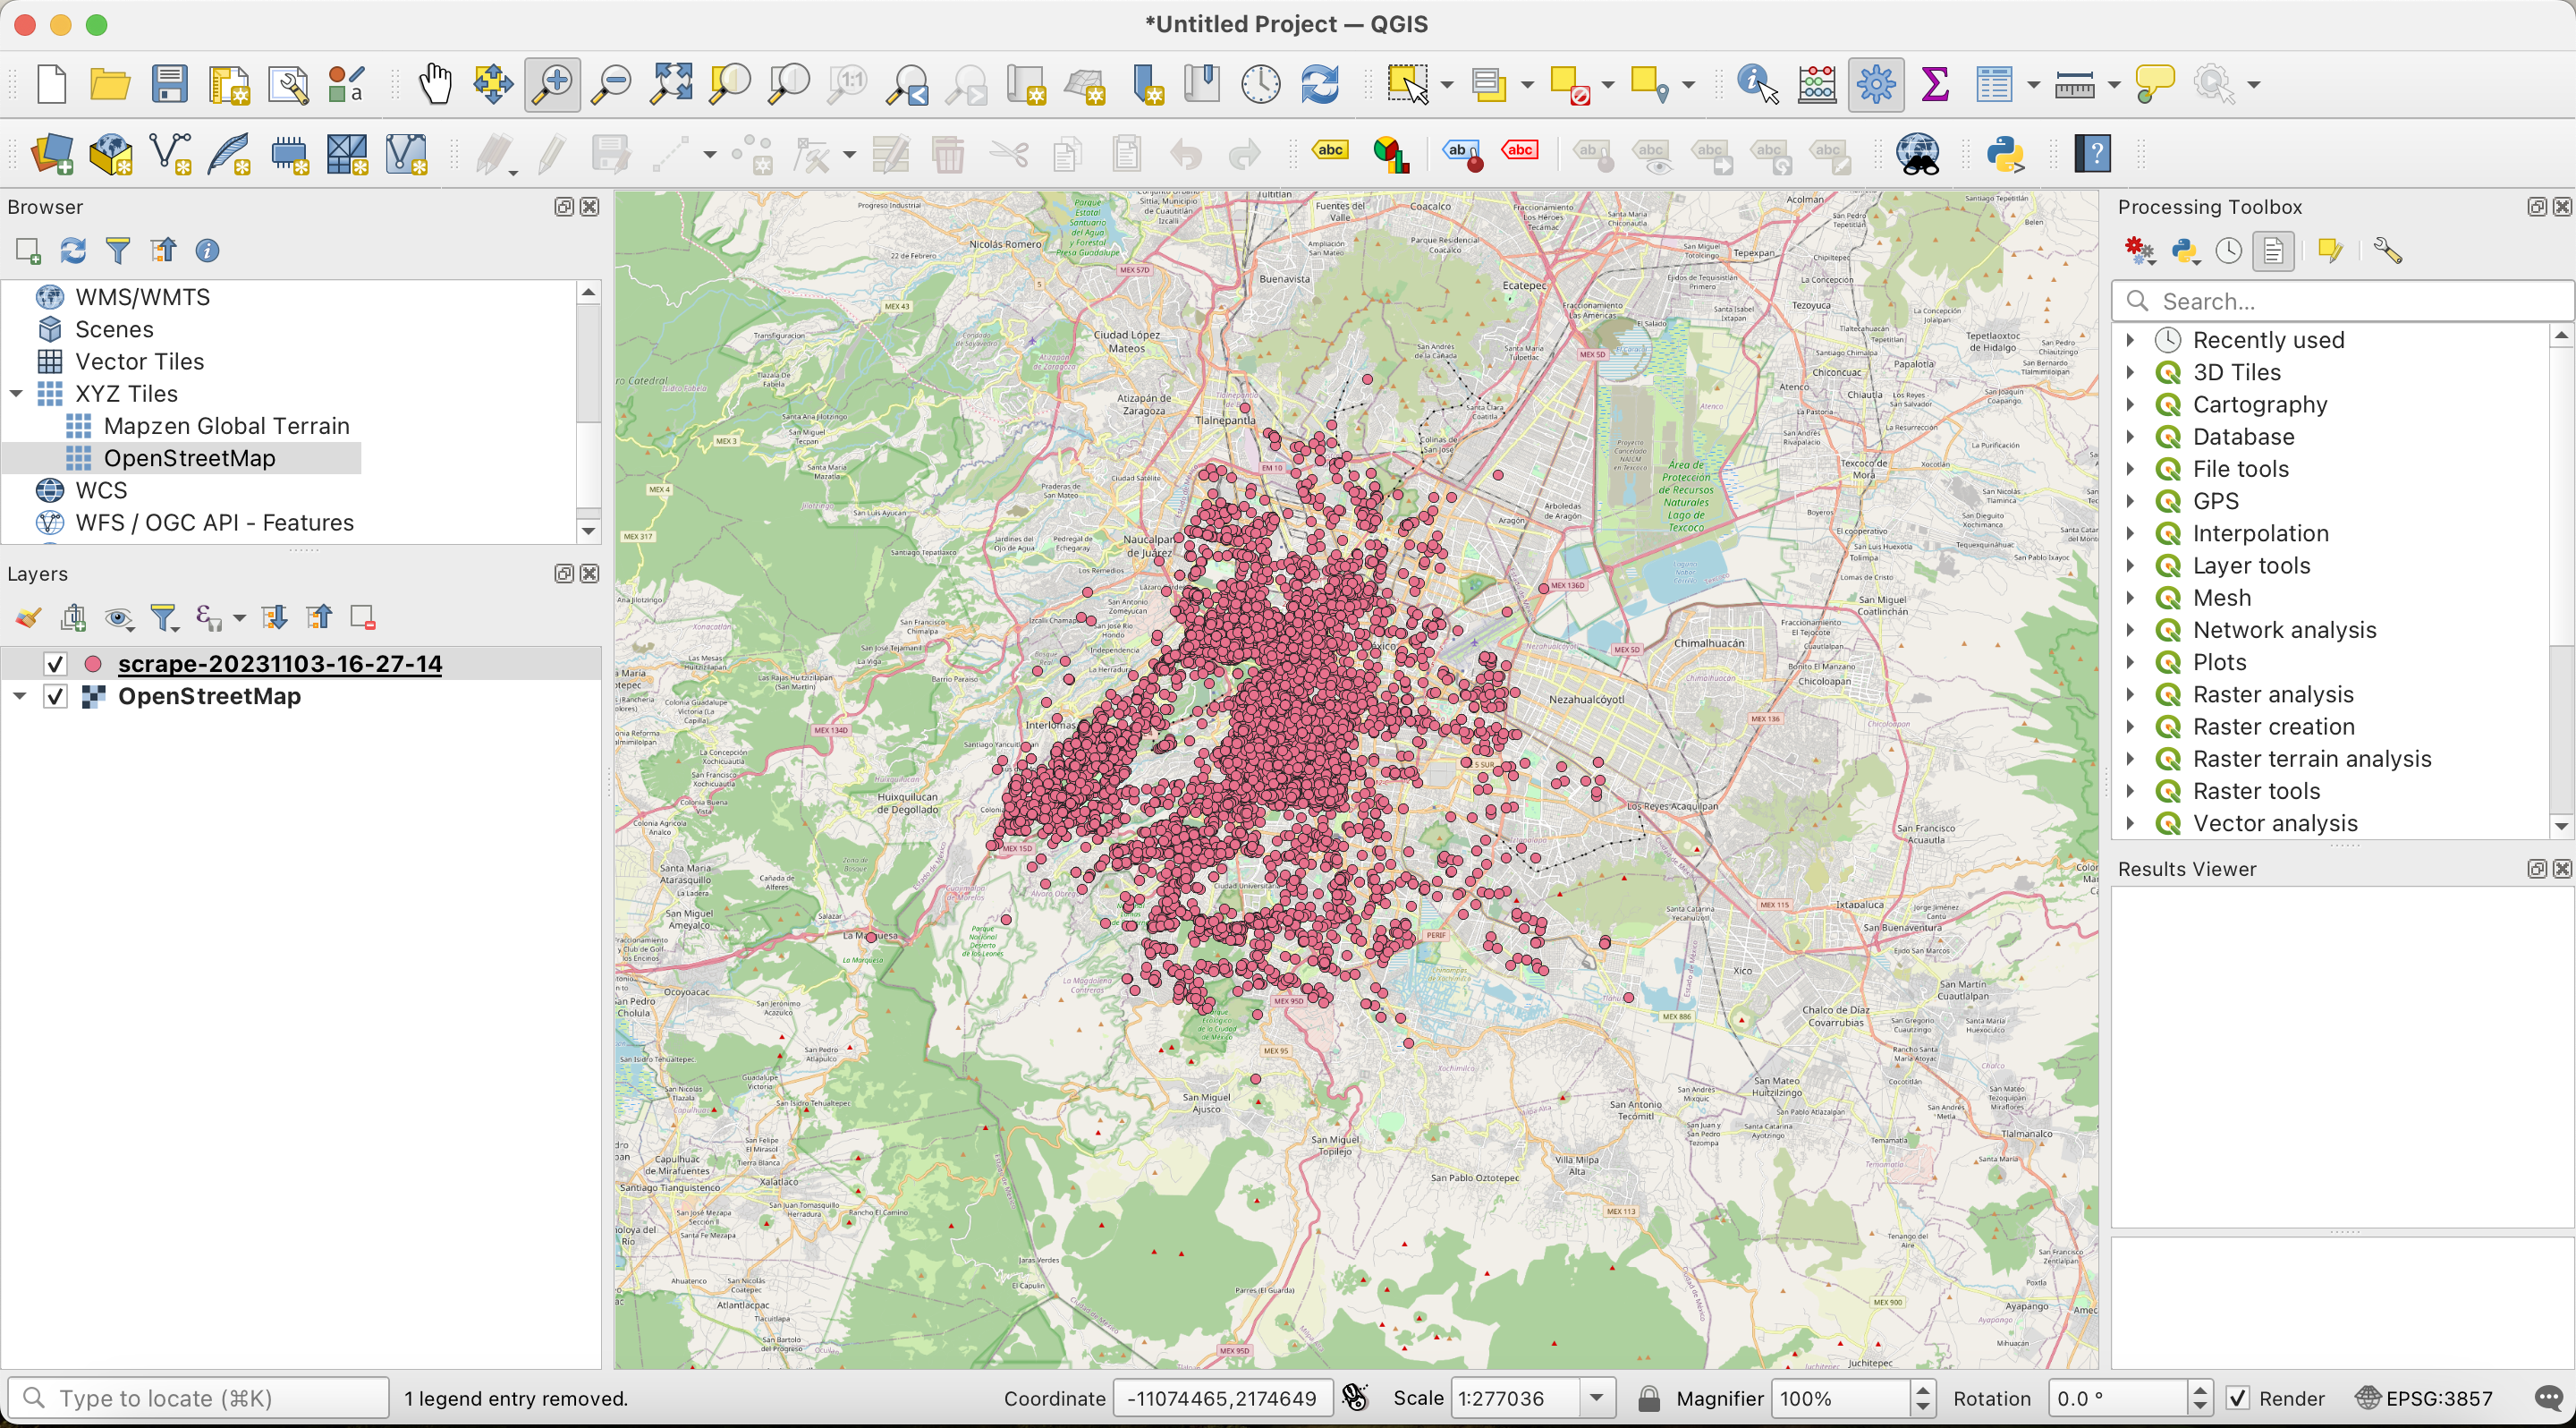
\includegraphics[width=0.9\textwidth]{imagenes/03-analisis/captura-qgis.png}
  \caption{Captura de pantalla de QGIS con los datos de bienes raíces de la Ciudad de México.}
  \label{fig:qgis}
\end{figure}

\subsubsection{React}
React es un marco de trabajo de código abierto desarrollado por Facebook para
crear interfaces de usuario. Se utiliza para manejar la capa de vista para aplicaciones
web y móviles. Una de las principales características de React es que utiliza
un enfoque basado en componentes para el desarrollo de aplicaciones. Con React,
los desarrolladores pueden crear componentes reutilizables que se pueden utilizar
para crear interfaces de usuario complejas. React también permite a los desarrolladores
crear interfaces de usuario declarativas. Esto significa que los desarrolladores
pueden escribir código que describa cómo debería ser la interfaz de usuario.
React se encarga de actualizar automáticamente la interfaz de usuario cuando
los datos cambian, lo que permite a los desarrolladores evitar tener que
escribir código adicional para actualizar la interfaz de usuario \cite{ReactLearn2023}.

Se eligió React debido a que es un marco de trabajo conocido por el equipo de
desarrollo, además de que, al ser de código abierto y alta popularidad, goza de
una gran cantidad de documentación, soporte y librerías que facilitan el desarrollo
de aplicaciones web.

\subsubsection{Material-UI}
Material-UI es una biblioteca de componentes de interfaz de usuario para React
que implementa el lenguaje de diseño de Google, Material Design, para la web.
Material-UI hace que el desarrollo de aplicaciones web sea más rápido y fácil \cite{mui_getting_started}.

Se decidió trabajar con Material-UI debido a que su implementación es conocida
por el equipo de desarrollo y su diseño es atractivo y moderno.

\subsubsection{Docker}
Docker es un proyecto de código abierto que automatiza el despliegue de aplicaciones
dentro de contenedores de software, proporcionando una capa adicional de abstracción
y automatización de virtualización de aplicaciones en múltiples sistemas operativos.
Docker utiliza características de aislamiento de recursos del kernel de Linux, como
cgroups y espacios de nombres (namespaces) para permitir que ``contenedores'' independientes
se ejecuten dentro de una sola instancia de Linux, evitando la sobrecarga de iniciar y
mantener máquinas virtuales (VMs) \cite{docker_overview}.

Se eligió Docker para empaquetar la aplicación web y facilitar su despliegue en
cualquier servidor, en nuestro caso, en la nube.

\subsection{Herramientas de Hardware}

En tanto a hardware se refiere, para el desarrollo de este proyecto se empleará
una computadora portátil con las siguientes características:

\begin{itemize}
  \item Procesador Apple M1 de 8 núcleos, 4 de rendimiento y 4 de eficiencia.
  \item GPU de 8 núcleos.
  \item 8 GB de memoria unificada.
  \item 256 GB de almacenamiento SSD.
  \item Pantalla Retina de 13 pulgadas con tecnología True Tone.
  \item Touch Bar y Touch ID.
  \item Dos puertos Thunderbolt / USB 4.
\end{itemize}

\subsubsection{Amazon Web Services}

Debido a que se pretende que la aplicación web sea accesible desde cualquier
dispositivo con acceso a internet, se consideró la posibilidad de emplear
servicios de computación en la nube para el despliegue de la aplicación web.
De los servicios de computación en la nube disponibles, se eligió Amazon Web
Services (AWS) debido a que es el servicio de computación en la nube más
popular y cuenta con una gran cantidad de documentación, soporte y librerías
que facilitan el despliegue de aplicaciones web.

Aunque el entrenamiento de los modelos de aprendizaje automático se realizará
en la computadora portátil mencionada anteriormente, el despliegue del sistema
final se realizará en un servicio de computación en la nube.

\section{Análisis Exploratorio de Datos}

El análisis exploratorio de datos es una parte fundamental del proceso de
minería de datos, ya que permite obtener información relevante sobre los datos
que se utilizarán para el entrenamiento del modelo de aprendizaje automático.
A su vez, permite identificar patrones, tendencias y
relaciones entre los datos, lo cual permite determinar la calidad de los datos
y la relevancia de las variables para el entrenamiento del modelo \cite{stephan2009exploratory}.

Debido a la naturaleza del proyecto, los datos que se utilizarán para el
entrenamiento del modelo de aprendizaje automático son datos de bienes raíces
georeferenciados mediante una latitud y longitud, por lo que el análisis
consistirá en un análisis exploratorio geoespacial y un análisis exploratorio
econométrico.

El conjunto de datos empleado para el análisis exploratorio de datos es un
conjunto de datos de bienes raíces de la Ciudad de México, el cual fue obtenido
de la plataforma Inmuebles24 \cite{inmuebles24}. Este conjunto de datos contiene
información sobre 40,000 anuncios de bienes raíces de la Ciudad de México,
los cuales fueron publicados hasta el 30 de Agosto de 2023. El conjunto de datos
se obtuvo únicamente para, a partir del presente análisis exploratorio de datos,
determinar la calidad de los datos y la relevancia de las variables para el
entrenamiento del modelo de aprendizaje automático. Para el desarrollo de la
plataforma final, se utilizará un conjunto de datos que incorpore los datos
extraídos durante el desarrollo del proyecto a bien de tener un conjunto de
datos más completo y actualizado.

\subsection{Análisis Exploratorio Geoespacial}

Como se mencionó, los datos tienen una componente geoespacial, por lo que es
importante realizar un análisis exploratorio geoespacial para poder obtener
información relevante. Dentro de este análisis se realizarán los siguientes
análisis:

\begin{itemize}
  \item Visualización de puntos de anuncios
  \item Mapa de densidad de anuncios por alcaldía
  \item Mapa de calor de precios
  \item Mapa de calor de número de recámaras
  \item Mapa de calor de número de baños
  \item Mapa de calor de metros cuadrados
  \item Mapa de calor de antigüedad
  \item Mapa de calor de estacionamientos
\end{itemize}

\subsubsection{Visualización de puntos de anuncios}

La visualización de puntos de anuncios permite representar individualmente cada
anuncio. Esto permite realizar un análisis de distribución geográfica y relación
con puntos de interés (parques, escuelas, centros comerciales, etc.). En la
Figura \ref{fig:visualizacion_puntos_anuncios} se muestra la visualización de
puntos de anuncios para el conjunto de datos de bienes raíces.

\begin{figure}[H]
  \centering
  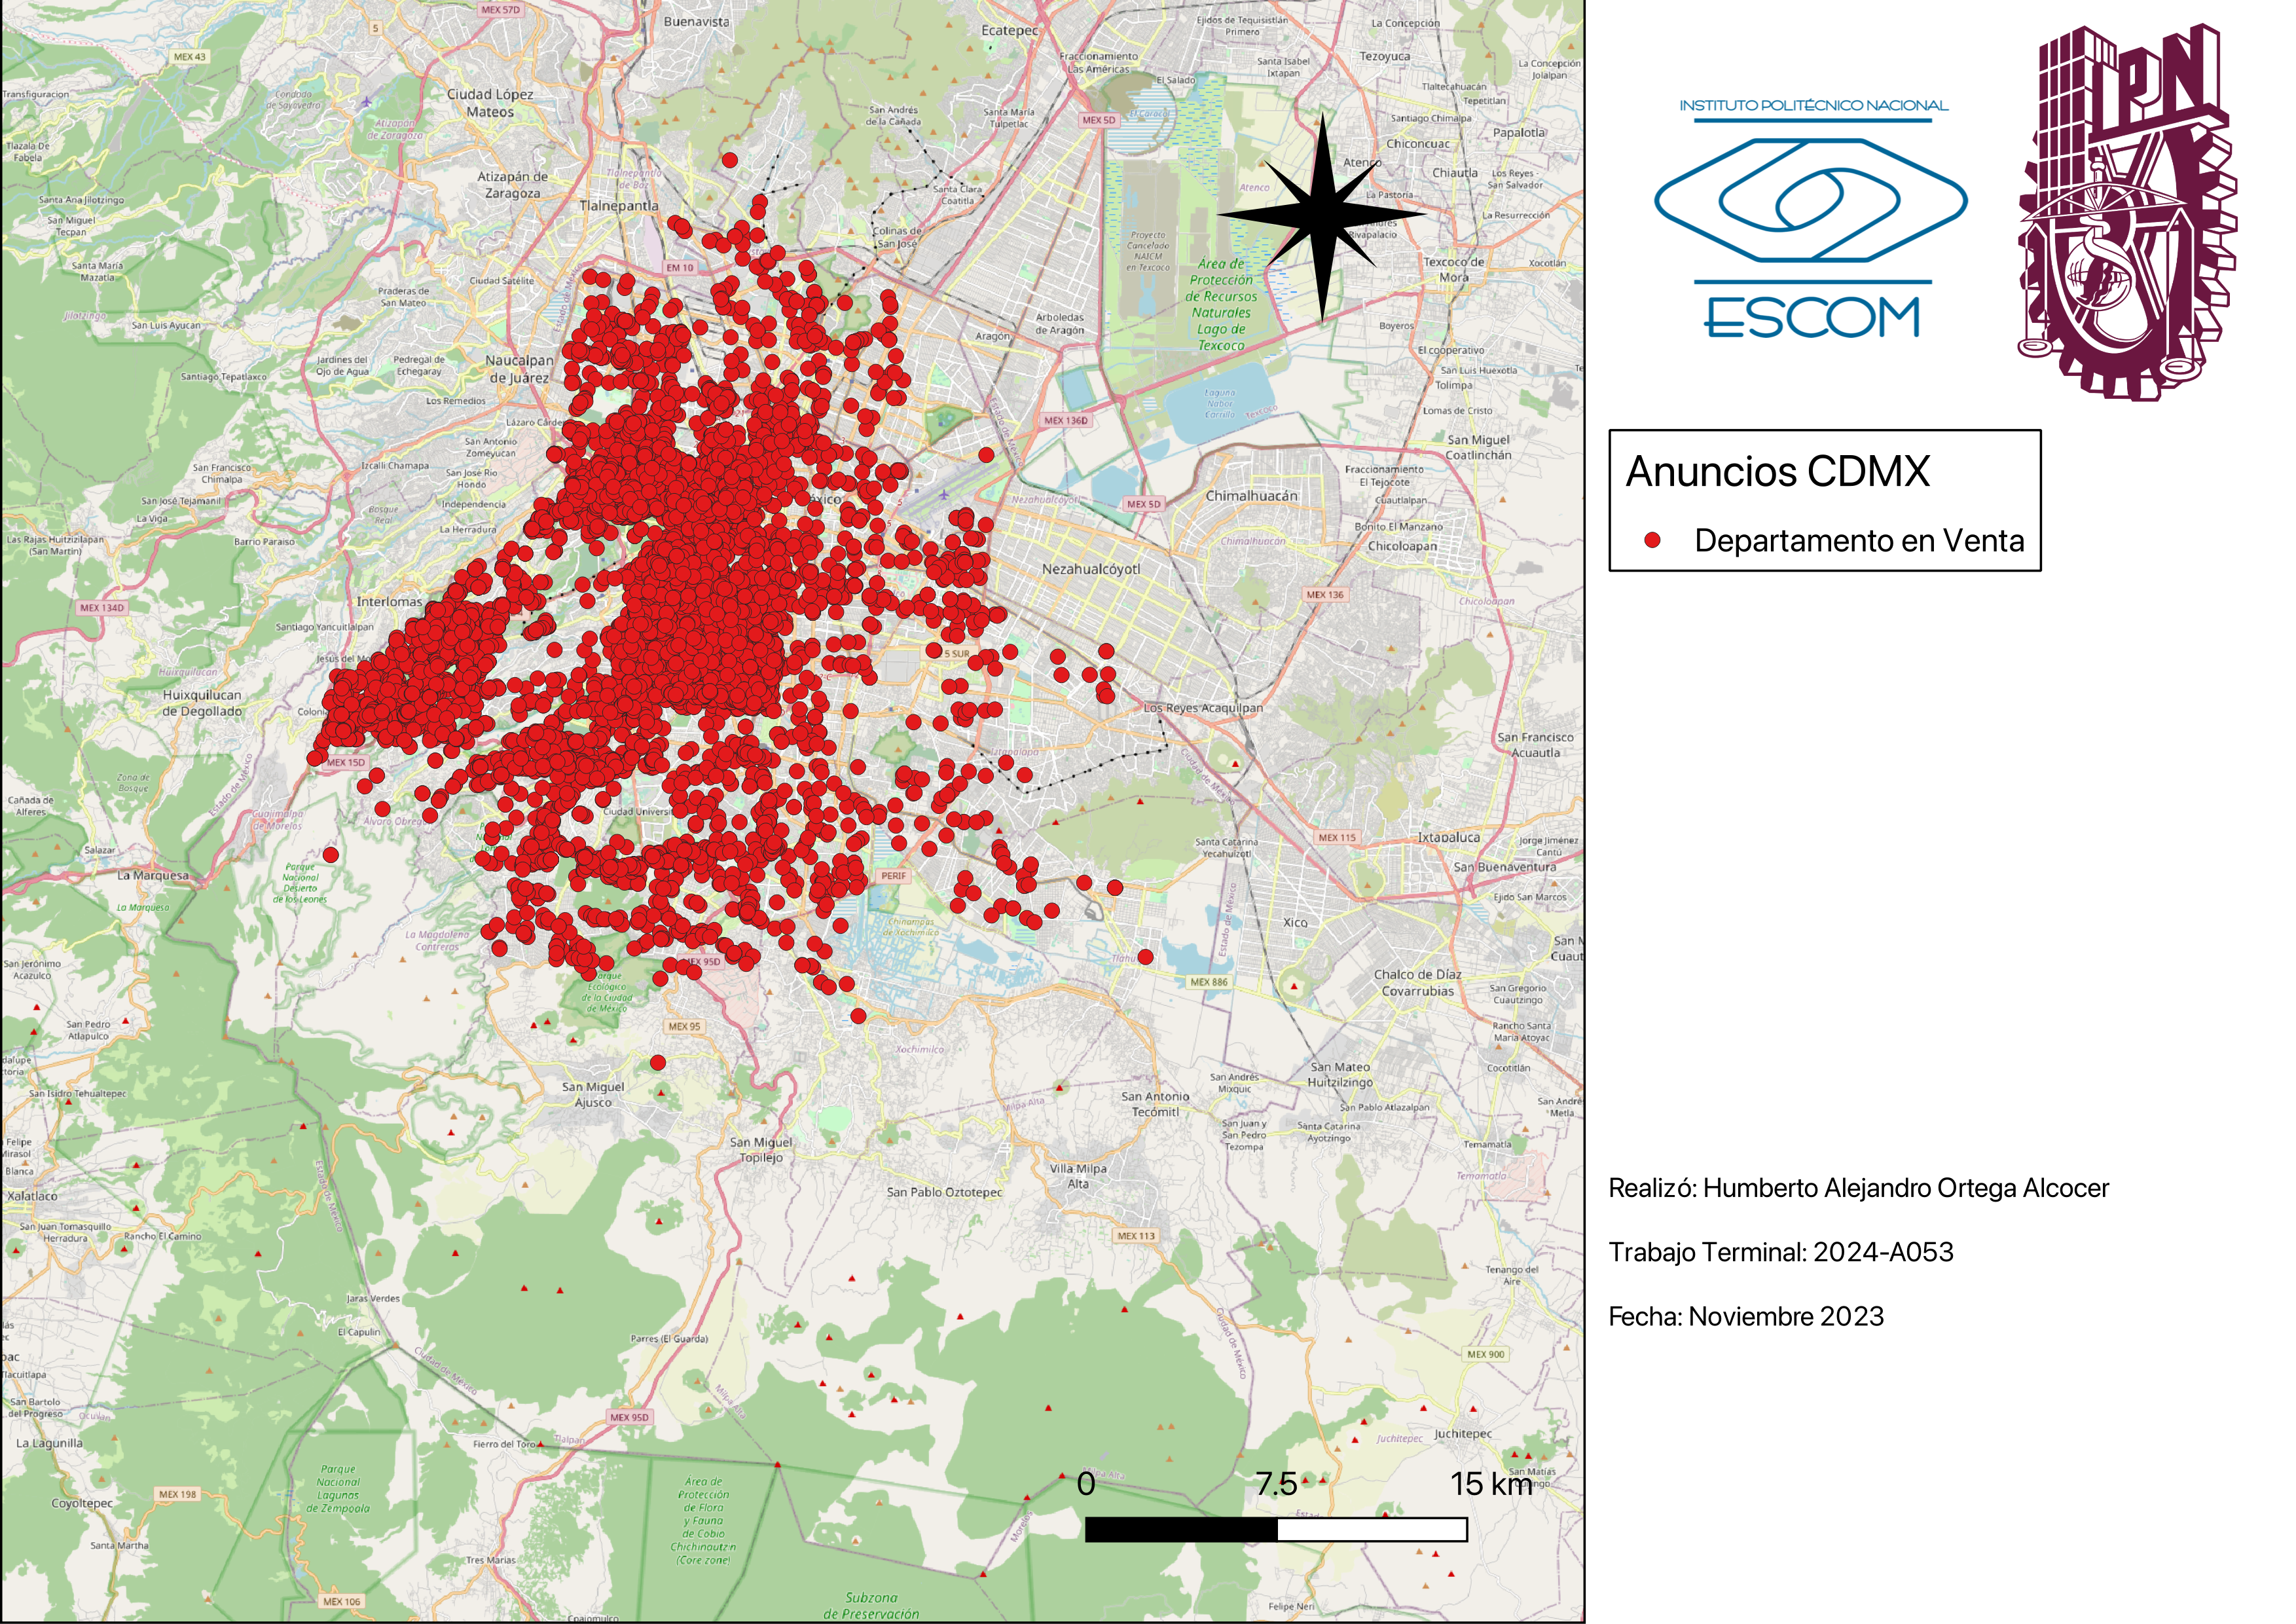
\includegraphics[width=0.8\textwidth]{imagenes/03-analisis/visualizacion-puntos-anuncios.png}
  \caption{Visualización de puntos de anuncios.}
  \label{fig:visualizacion_puntos_anuncios}
\end{figure}

De aquí, podemos derivar las siguientes conclusiones:

\begin{itemize}
  \item Los anuncios no se encuentran distribuidos de manera uniforme en toda la
  Ciudad de México.
  \item Los anuncios se encuentran distribuidos de manera uniforme en las
  alcaldías Cuauhtémoc, Benito Juárez y Miguel Hidalgo.
\item En las alcaldías Milpa Alta y Xochimilco existen pocos anuncios debido a
  que son zonas con poca densidad de población y muchos tratos aún se realizan
    de manera tradicional (sin el uso de plataformas online).
\end{itemize}

\subsubsection{Mapa de densidad de anuncios por alcaldía}

El mapa de densidad de anuncios permite visualizar la concentración de
anuncios en las diferentes alcaldías de la CDMX. Esto permite identificar las áreas con alta y baja
densidad de anuncios y posibles factores (desarrollo urbano, demanda, etc.). En
la Figura \ref{fig:mapa_calor_densidad_anuncios} se muestra el mapa de calor de
densidad de anuncios para el conjunto de datos de bienes raíces.

\begin{figure}[H]
  \centering
  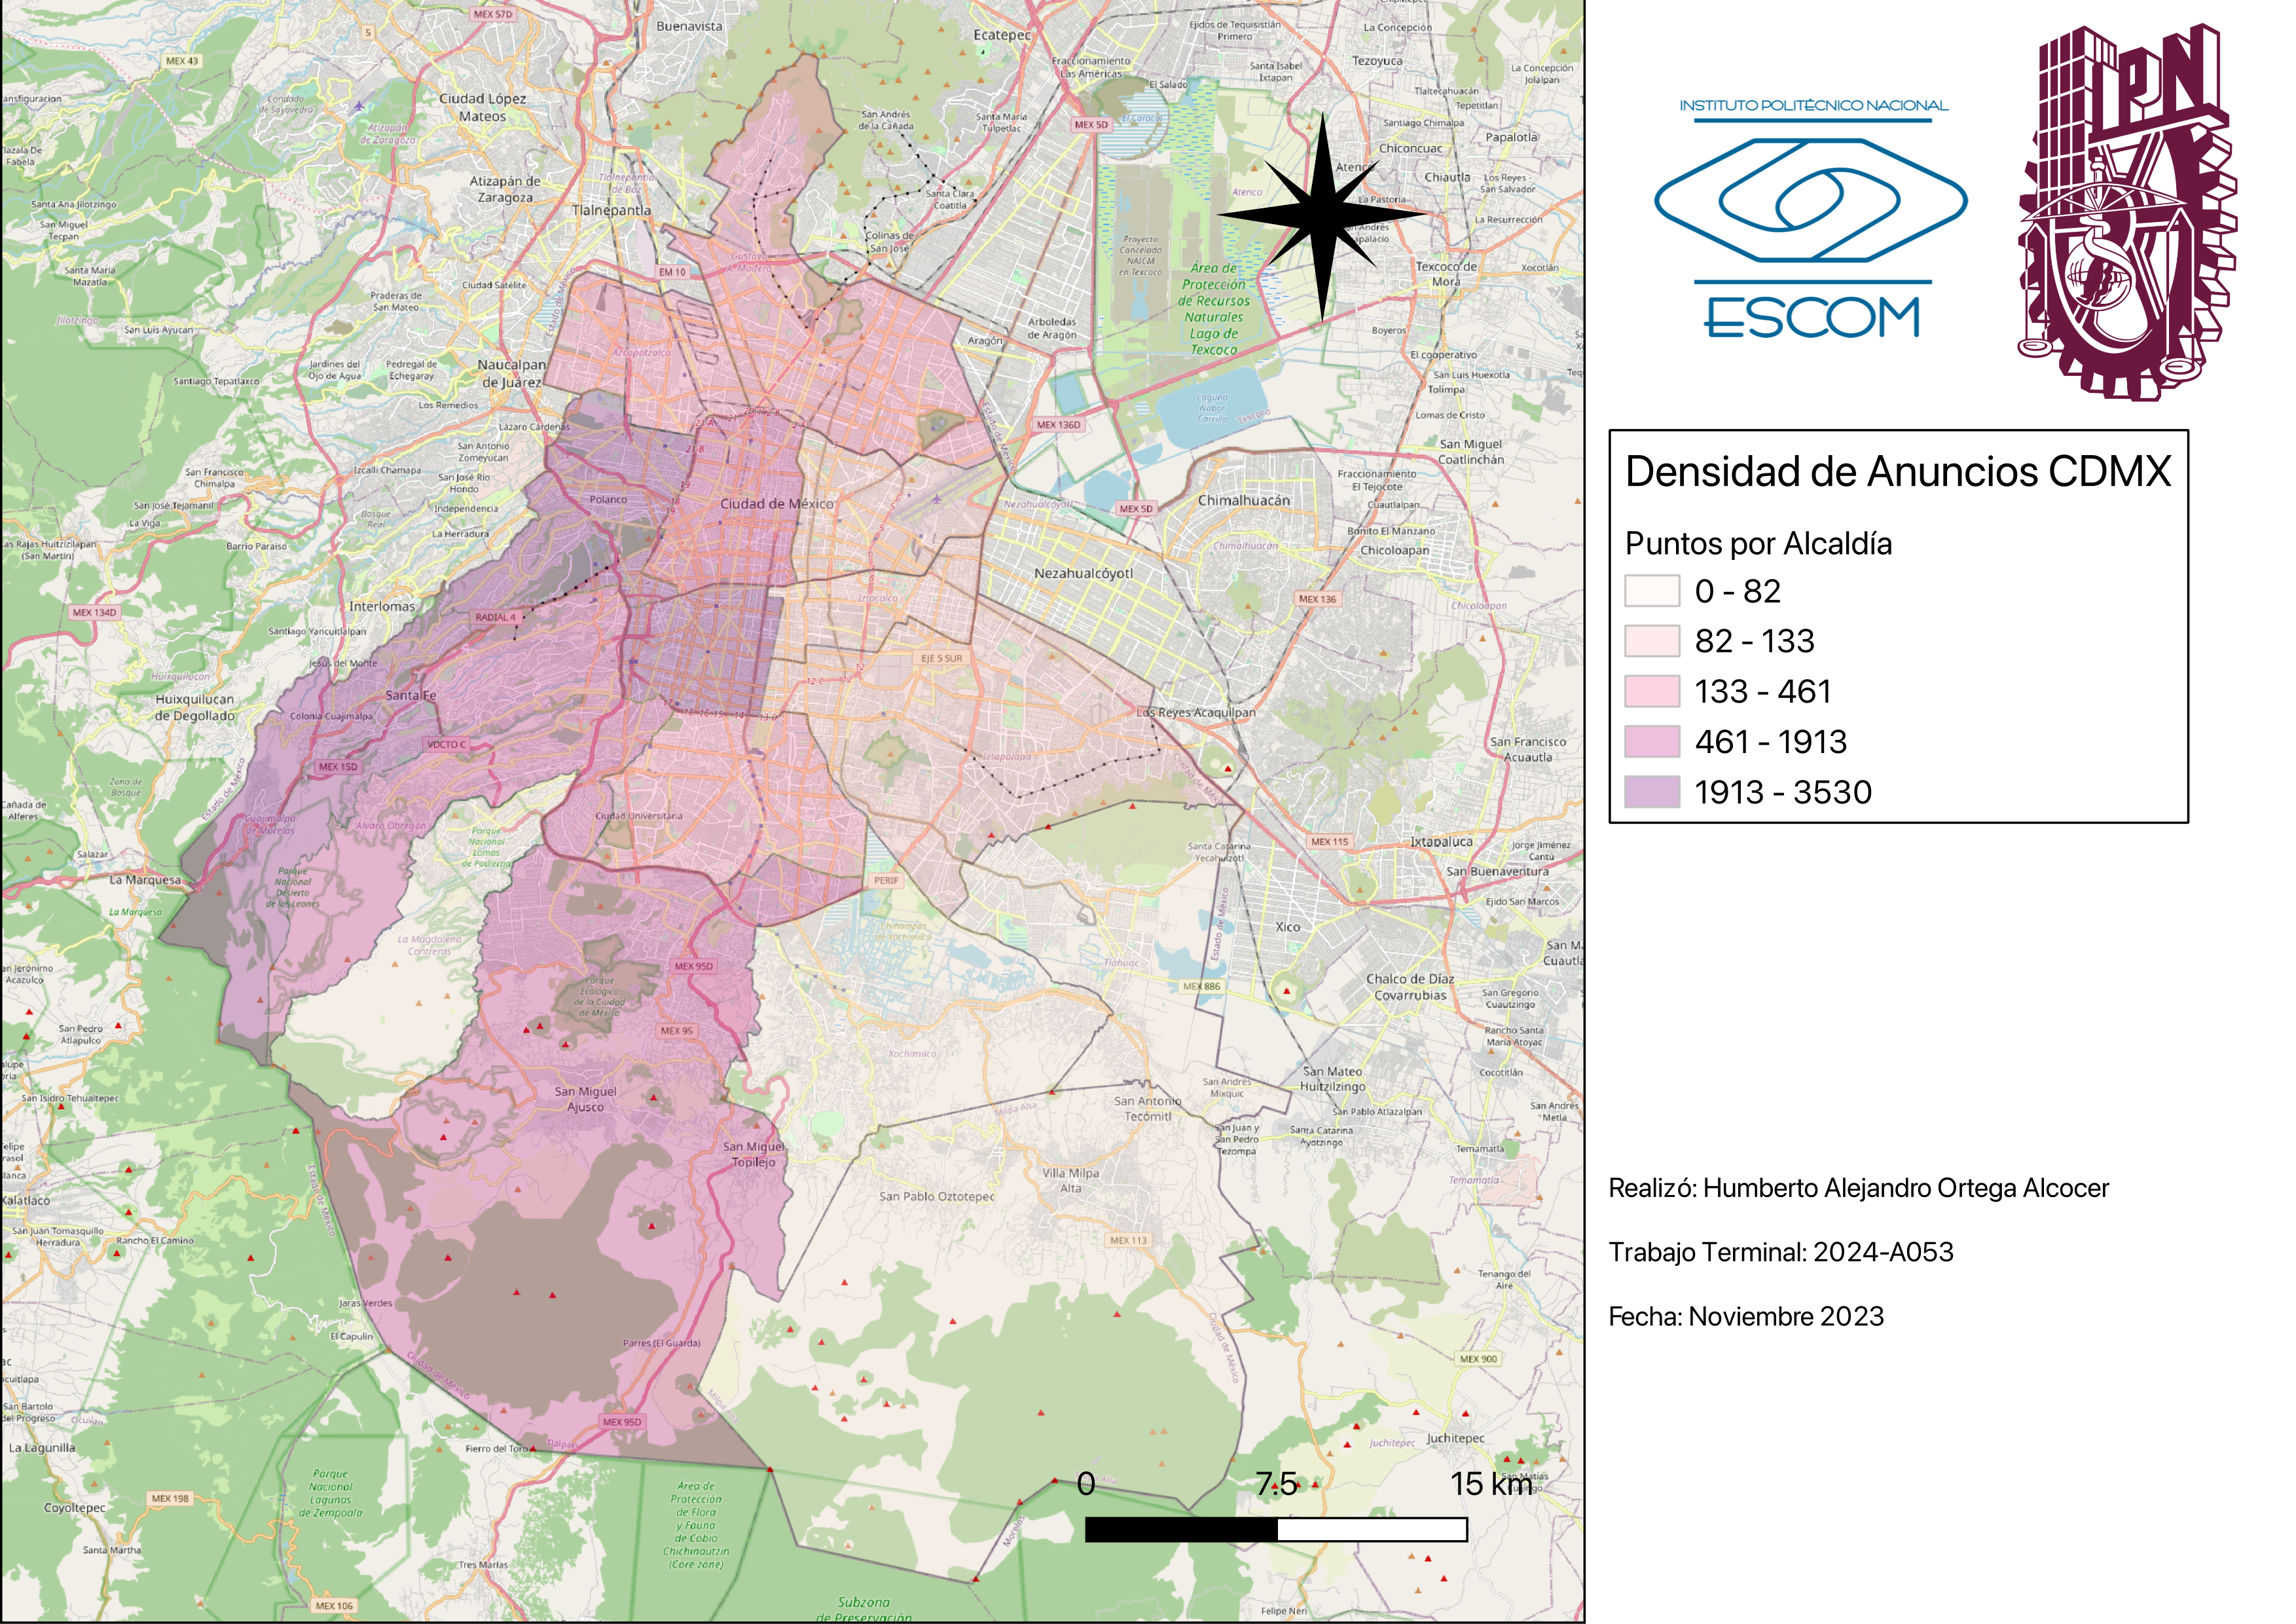
\includegraphics[width=0.8\textwidth]{imagenes/03-analisis/mapa-densidad-anuncios.png}
  \caption{Mapa de de densidad de anuncios por alcaldía.}
  \label{fig:mapa_calor_densidad_anuncios}
\end{figure}

De aquí, podemos derivar las siguientes conclusiones:

\begin{itemize}
  \item Las zonas con mayor densidad de anuncios se encuentran en la zona centro
  de la Ciudad de México, en las alcaldías Cuauhtémoc y Miguel Hidalgo.
  \item Las zonas con menor densidad de anuncios se encuentran en la zona sur
  de la Ciudad de México, en las alcaldías Tlalpan, Xochimilco y Milpa Alta.
\end{itemize}

Los datos correspondientes al mapa de la Figura \ref{fig:mapa_calor_densidad_anuncios}
se muestran en el Cuadro \ref{table:mapa_calor_densidad_anuncios}.

\begin{table}[H]
\centering
\begin{tabular}{|l|l|}
\hline
\rowcolor{azulclaro}
%\centering\textbf{Alcaldía} & \centering\textbf{Cantidad de Anuncios}\arraybackslash \\
\multicolumn{1}{|c|}{\textbf{Alcaldía}} & \multicolumn{1}{c|}{\textbf{Cantidad de Anuncios}} \\
\hline
Benito Juárez & 3530 \\
\hline
Miguel Hidalgo & 3114 \\
\hline
Cuajimalpa de Morelos & 2246 \\
\hline
Cuauhtémoc & 1913 \\
\hline
Álvaro Obregón & 1711 \\
\hline
Tlalpan & 483 \\
\hline
Coyoacán & 461 \\
\hline
Azcapotzalco & 301 \\
\hline
Gustavo A. Madero & 191 \\
\hline
Iztacalco & 133 \\
\hline
Venustiano Carranza & 127 \\
\hline
Iztapalapa & 117 \\
\hline
La Magdalena Contreras & 82 \\
\hline
Tláhuac & 29 \\
\hline
Xochimilco & 16 \\
\hline
Milpa Alta & 0 \\
\hline
\end{tabular}
\caption{Datos correspondientes al número de anuncios encontrados por alcaldía.}
\label{table:mapa_calor_densidad_anuncios}
\end{table}
\subsubsection{Mapa de calor de precios}

El mapa de calor de precios permite visualizar cómo se distribuyen los precios
en diferentes áreas. Esto permite identificar las zonas con precios más altos o
más bajos y posibles razones (ubicación, accesibilidad, etc.). En la Figura
\ref{fig:mapa_calor_precios} se muestra el mapa de calor de precios para el
conjunto de datos de bienes raíces.

\begin{figure}[H]
  \centering
  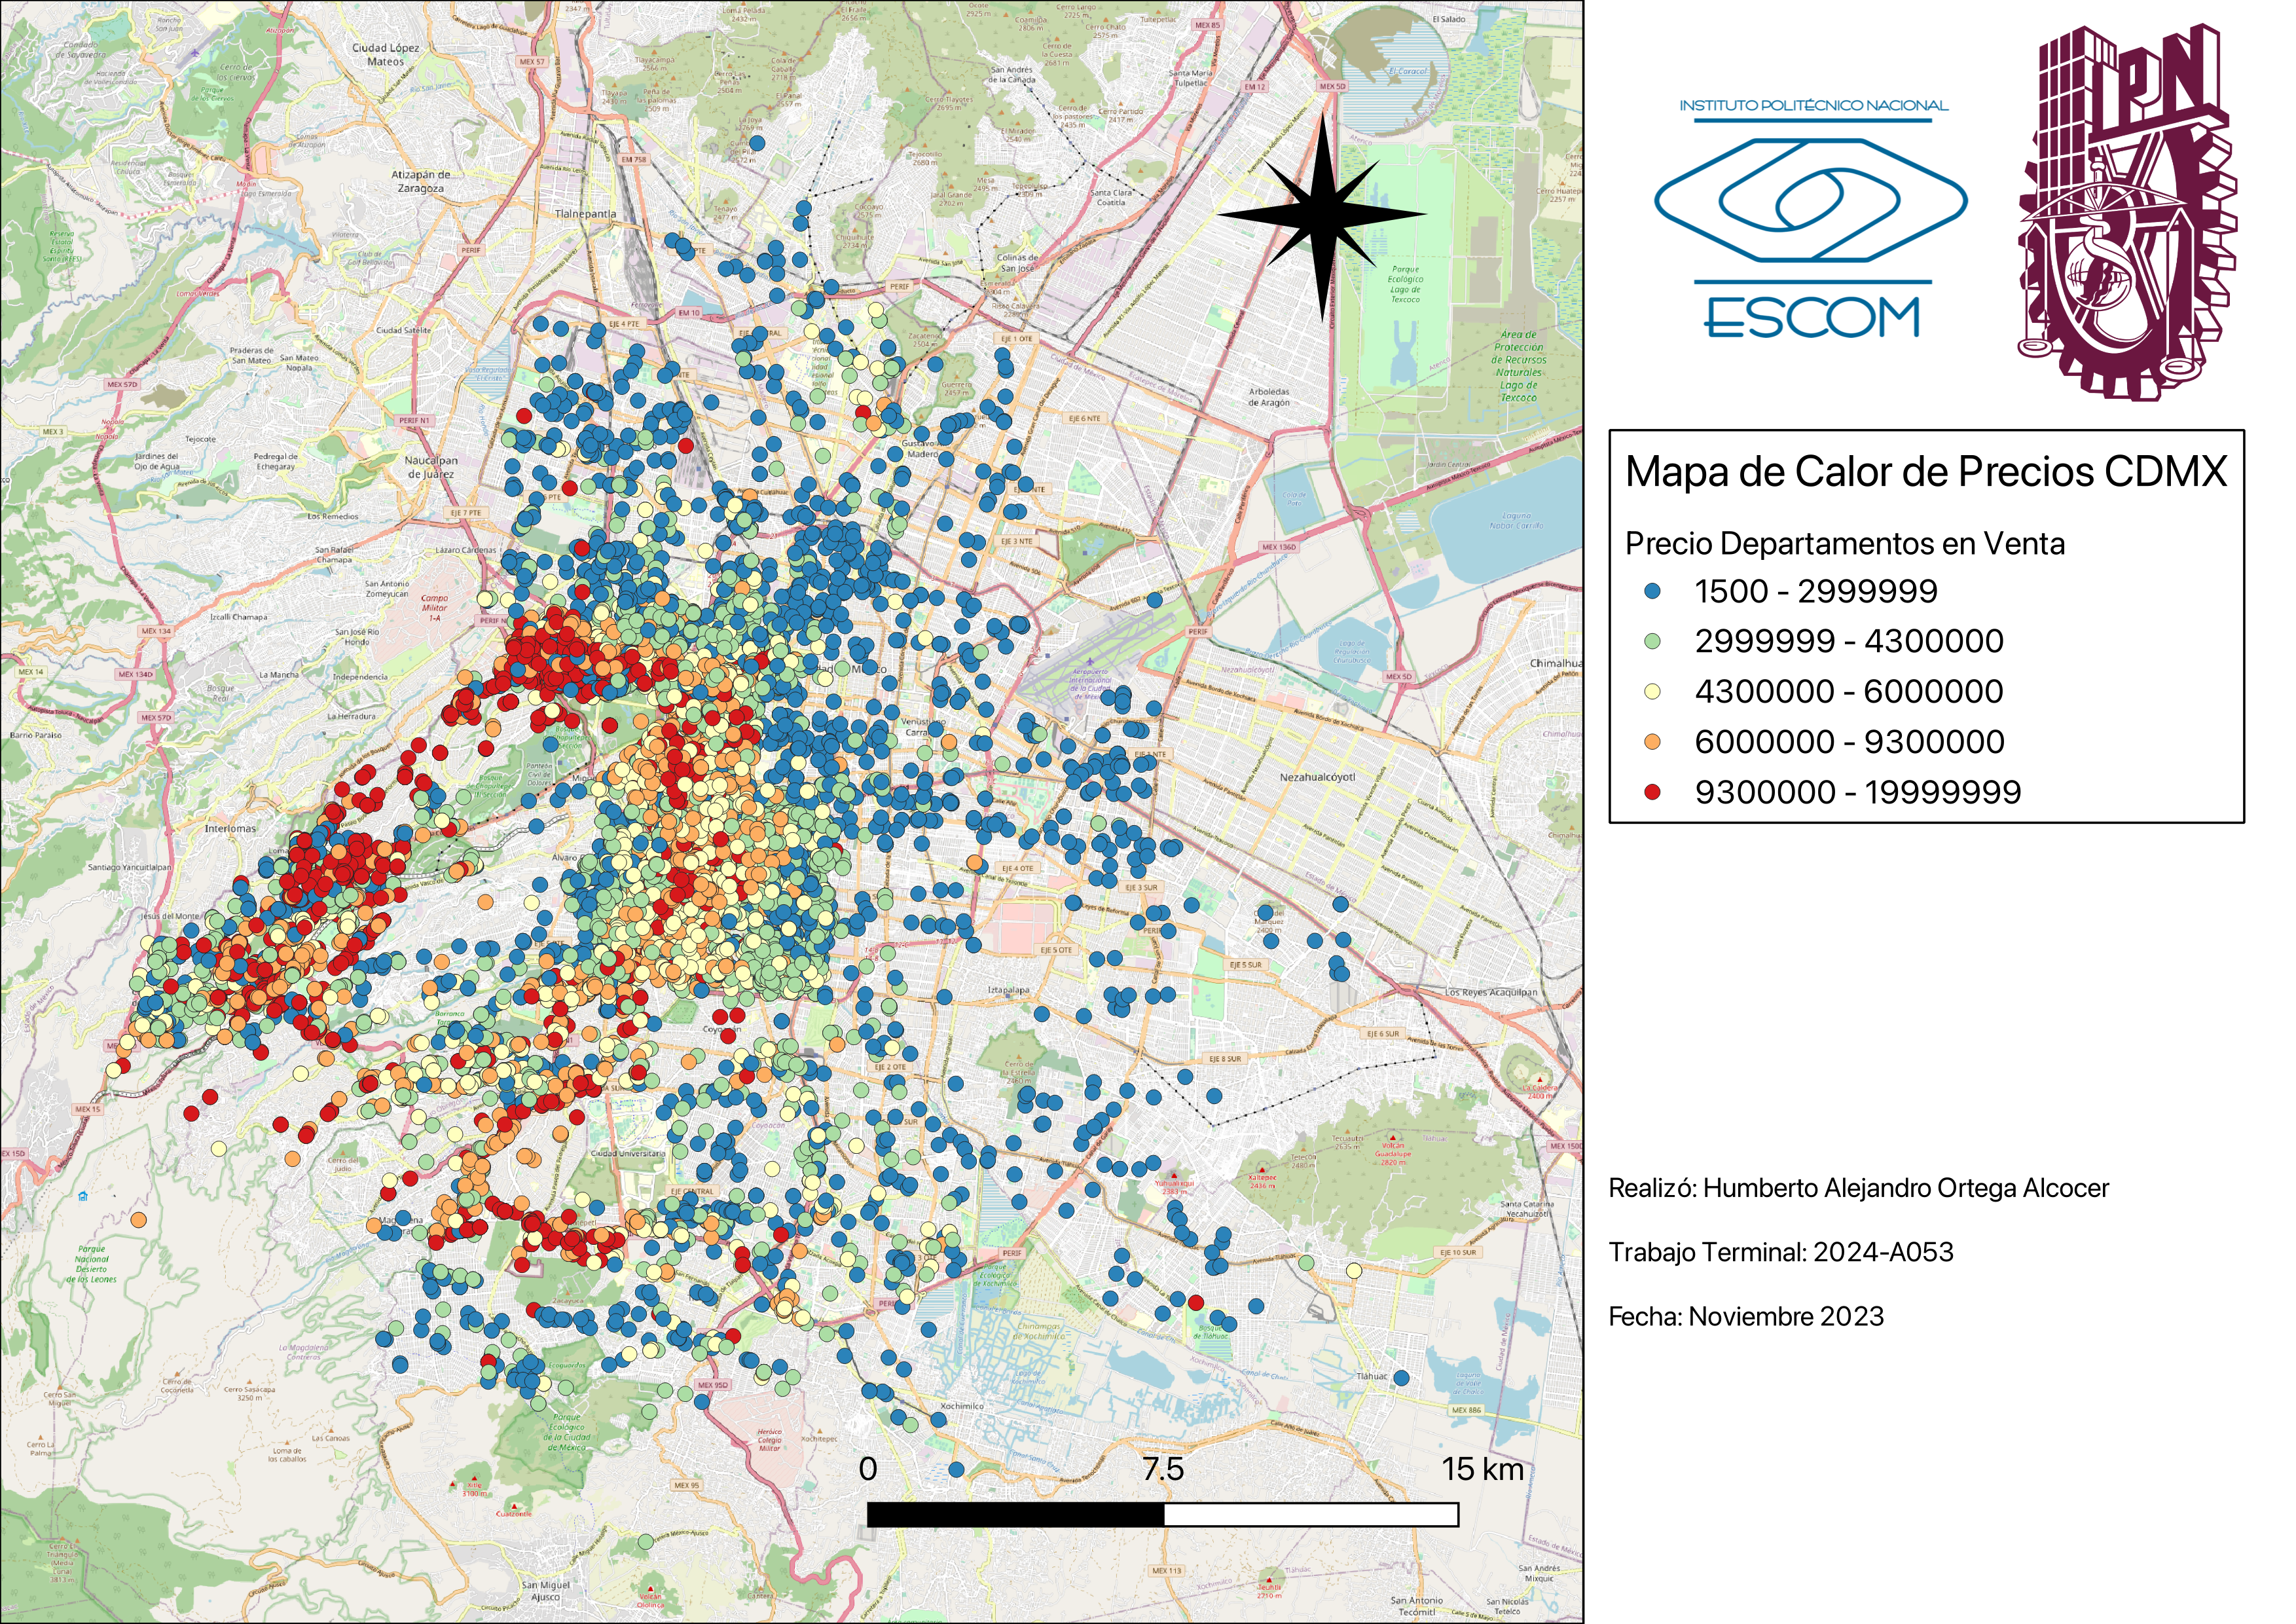
\includegraphics[width=0.9\textwidth]{imagenes/03-analisis/mapa-densidad-precio.png}
  \caption{Mapa de calor de precios.}
  \label{fig:mapa_calor_precios}
\end{figure}

De aquí, podemos derivar las siguientes conclusiones:

\begin{itemize}
  \item Los precios más altos se encuentran en la zona centro de la Ciudad de
  México, en las alcaldías Cuauhtémoc y Miguel Hidalgo.
  \item Los precios más bajos se encuentran en la zona sur de la Ciudad de
  México, en las alcaldías Tlalpan, Xochimilco y Milpa Alta.
\item Los precios más altos se encuentran en las zonas con mayor densidad de
  vegetación, como el Bosque de Chapultepec, el Parque Ecológico de Xochimilco
  y el Parque Ecológico de la Ciudad de México.
\end{itemize}

\subsubsection{Mapa de calor de número de recámaras}

El mapa de calor de número de recámaras permite visualizar cómo se distribuyen
los anuncios según el número de recámaras. Esto permite identificar las zonas
con mayor y menor número de recámaras y analizar si el precio es un factor
determinante en el número de recámaras. En la Figura \ref{fig:mapa_calor_recamaras}
se muestra el mapa de calor de número de recámaras para el conjunto de datos de
bienes raíces.

\begin{figure}[H]
  \centering
  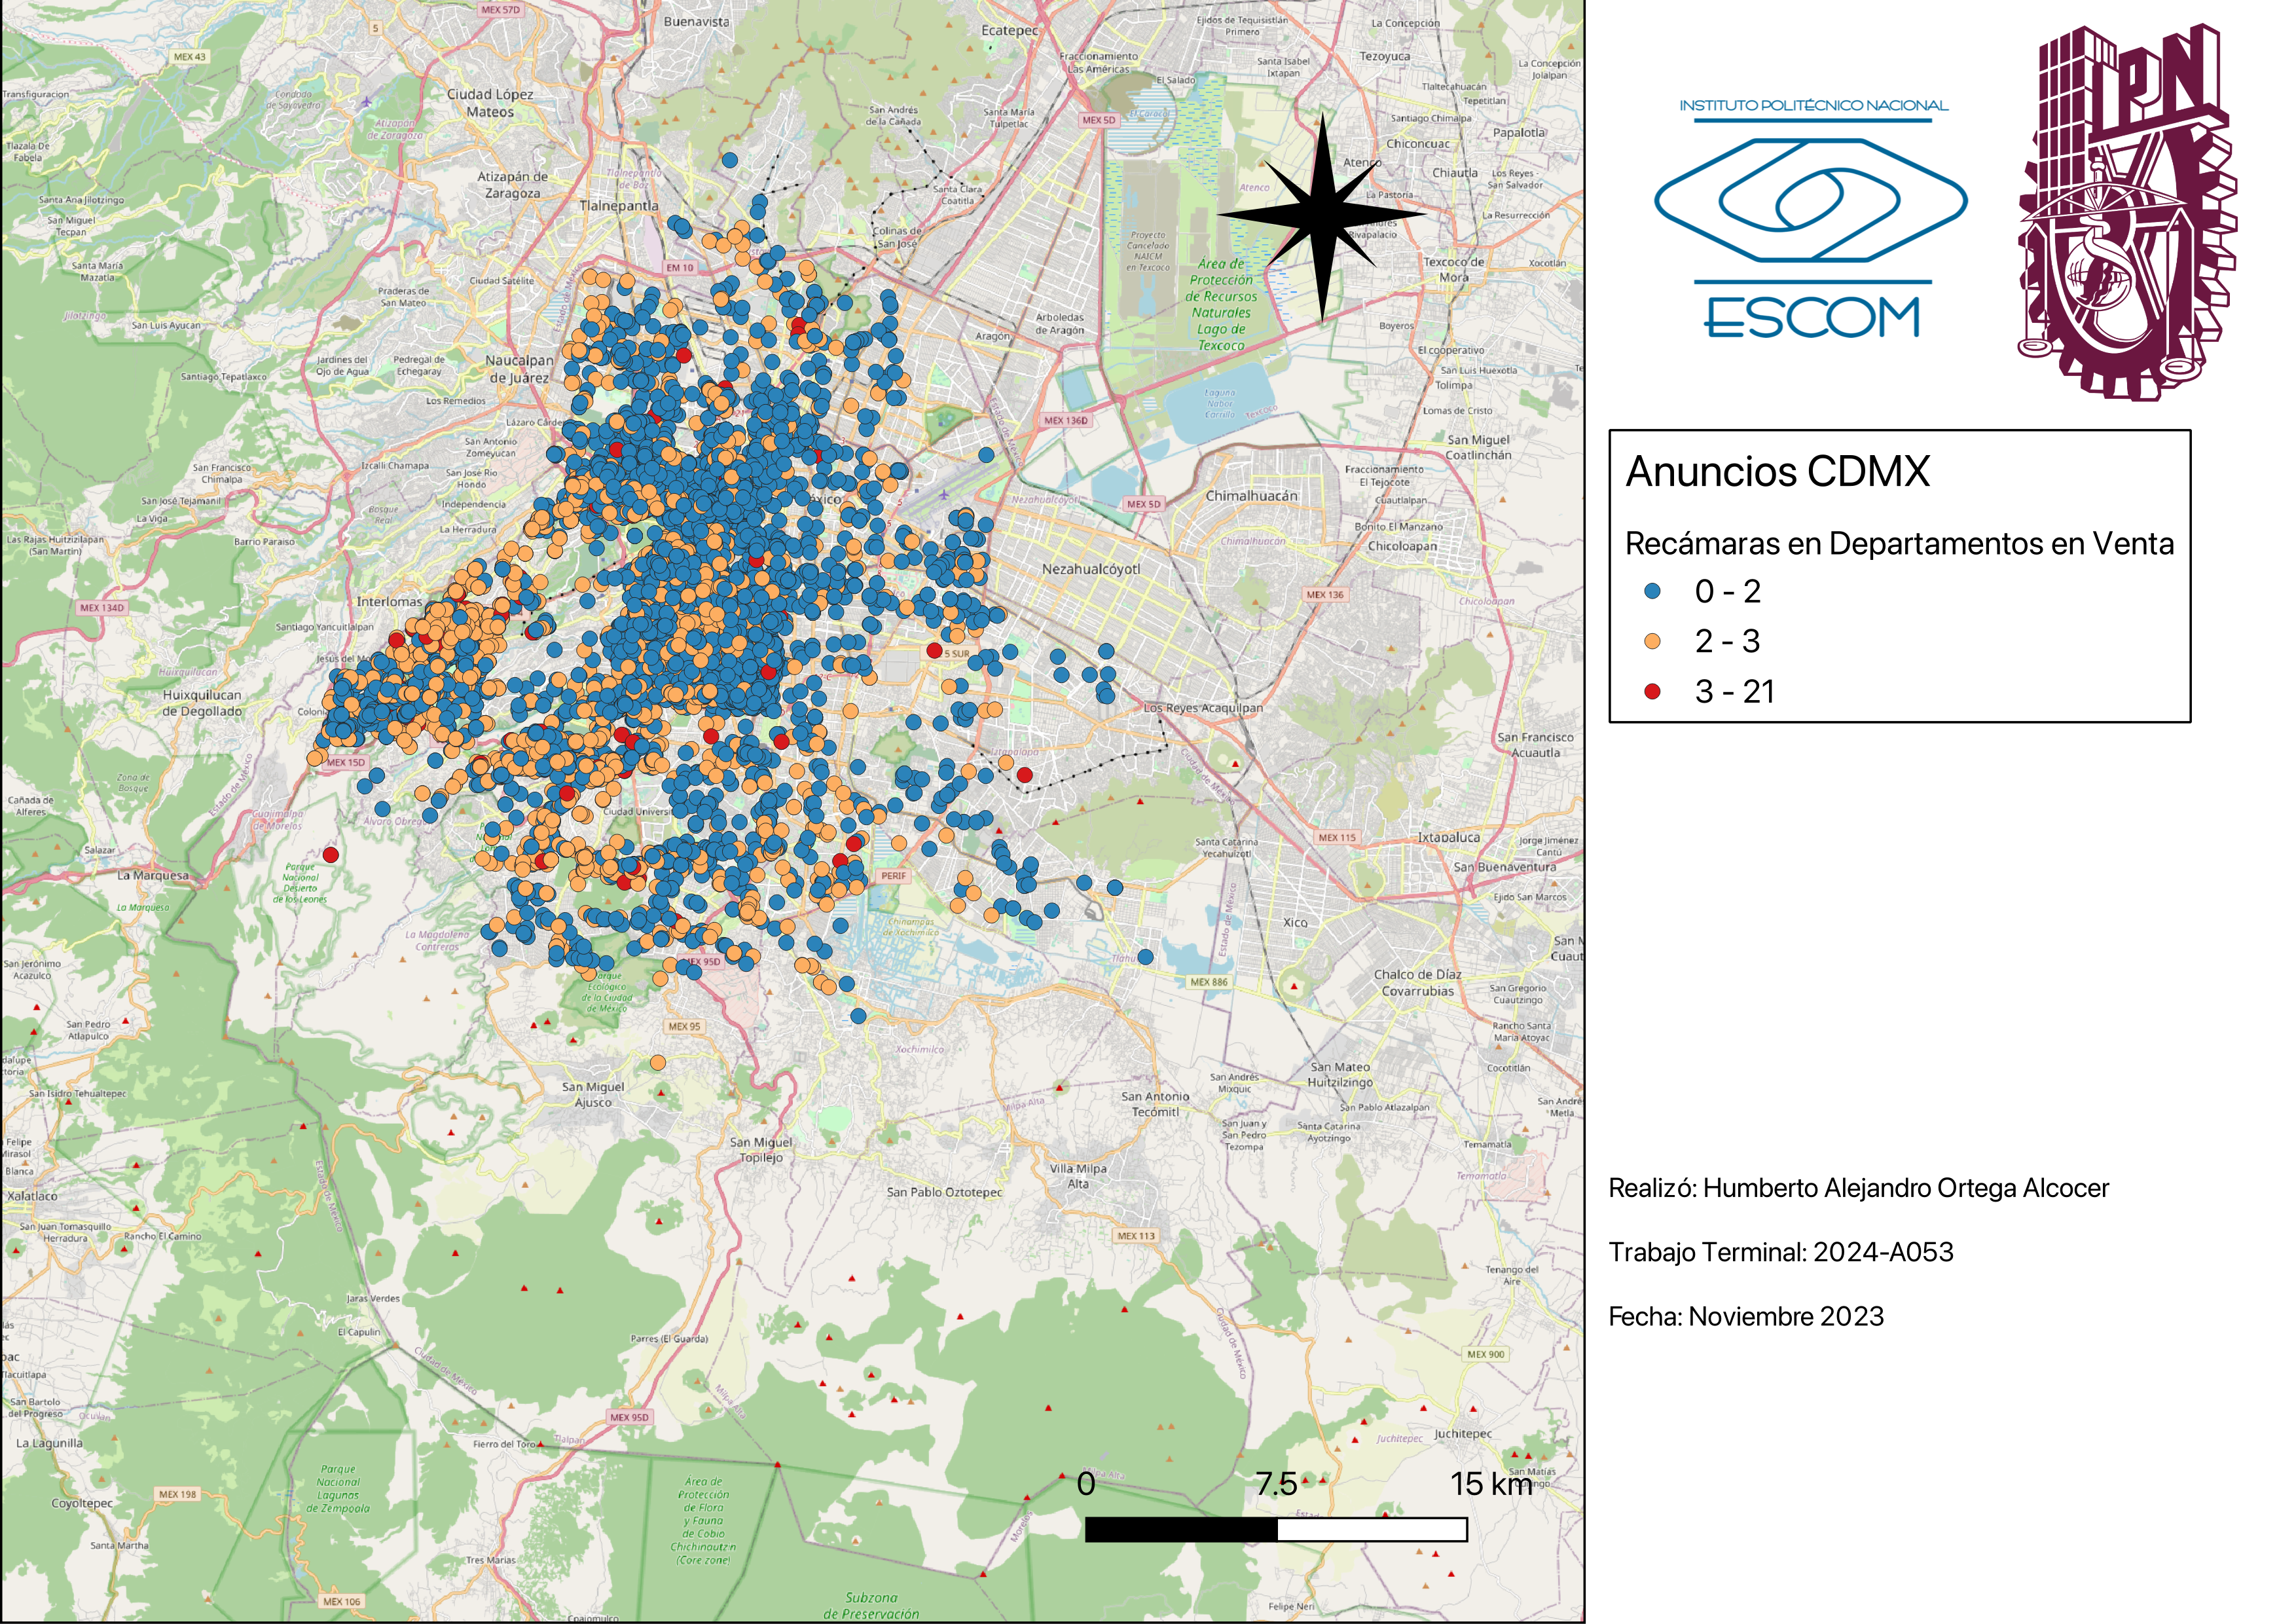
\includegraphics[width=0.9\textwidth]{imagenes/03-analisis/mapa-densidad-recamaras.png}
  \caption{Mapa de calor de número de recámaras.}
  \label{fig:mapa_calor_recamaras}
\end{figure}

De aquí, podemos derivar las siguientes conclusiones:

\begin{itemize}
  \item La gran mayoría de los departamentos en la Ciudad de México tienen 2 o
  3 recámaras.
  \item Los departamentos con 1 recámara se encuentran en las zonas con mayor
  densidad de población, como la zona centro de la Ciudad de México.
  \item Los departamentos con 4 o más recámaras se encuentran en las zonas con
  mayor precio, como la zona poniene de la Ciudad de México.
\end{itemize}

\subsubsection{Mapa de calor de número de baños}

Los baños nos indican la disponibilidad de servicios sanitarios en el inmueble,
así como un aproximado del número de personas que podrían habitar el mismo. En
la Figura \ref{fig:mapa_calor_banos} se muestra el mapa de calor de número de
baños para el conjunto de datos de bienes raíces.

\begin{figure}[H]
  \centering
  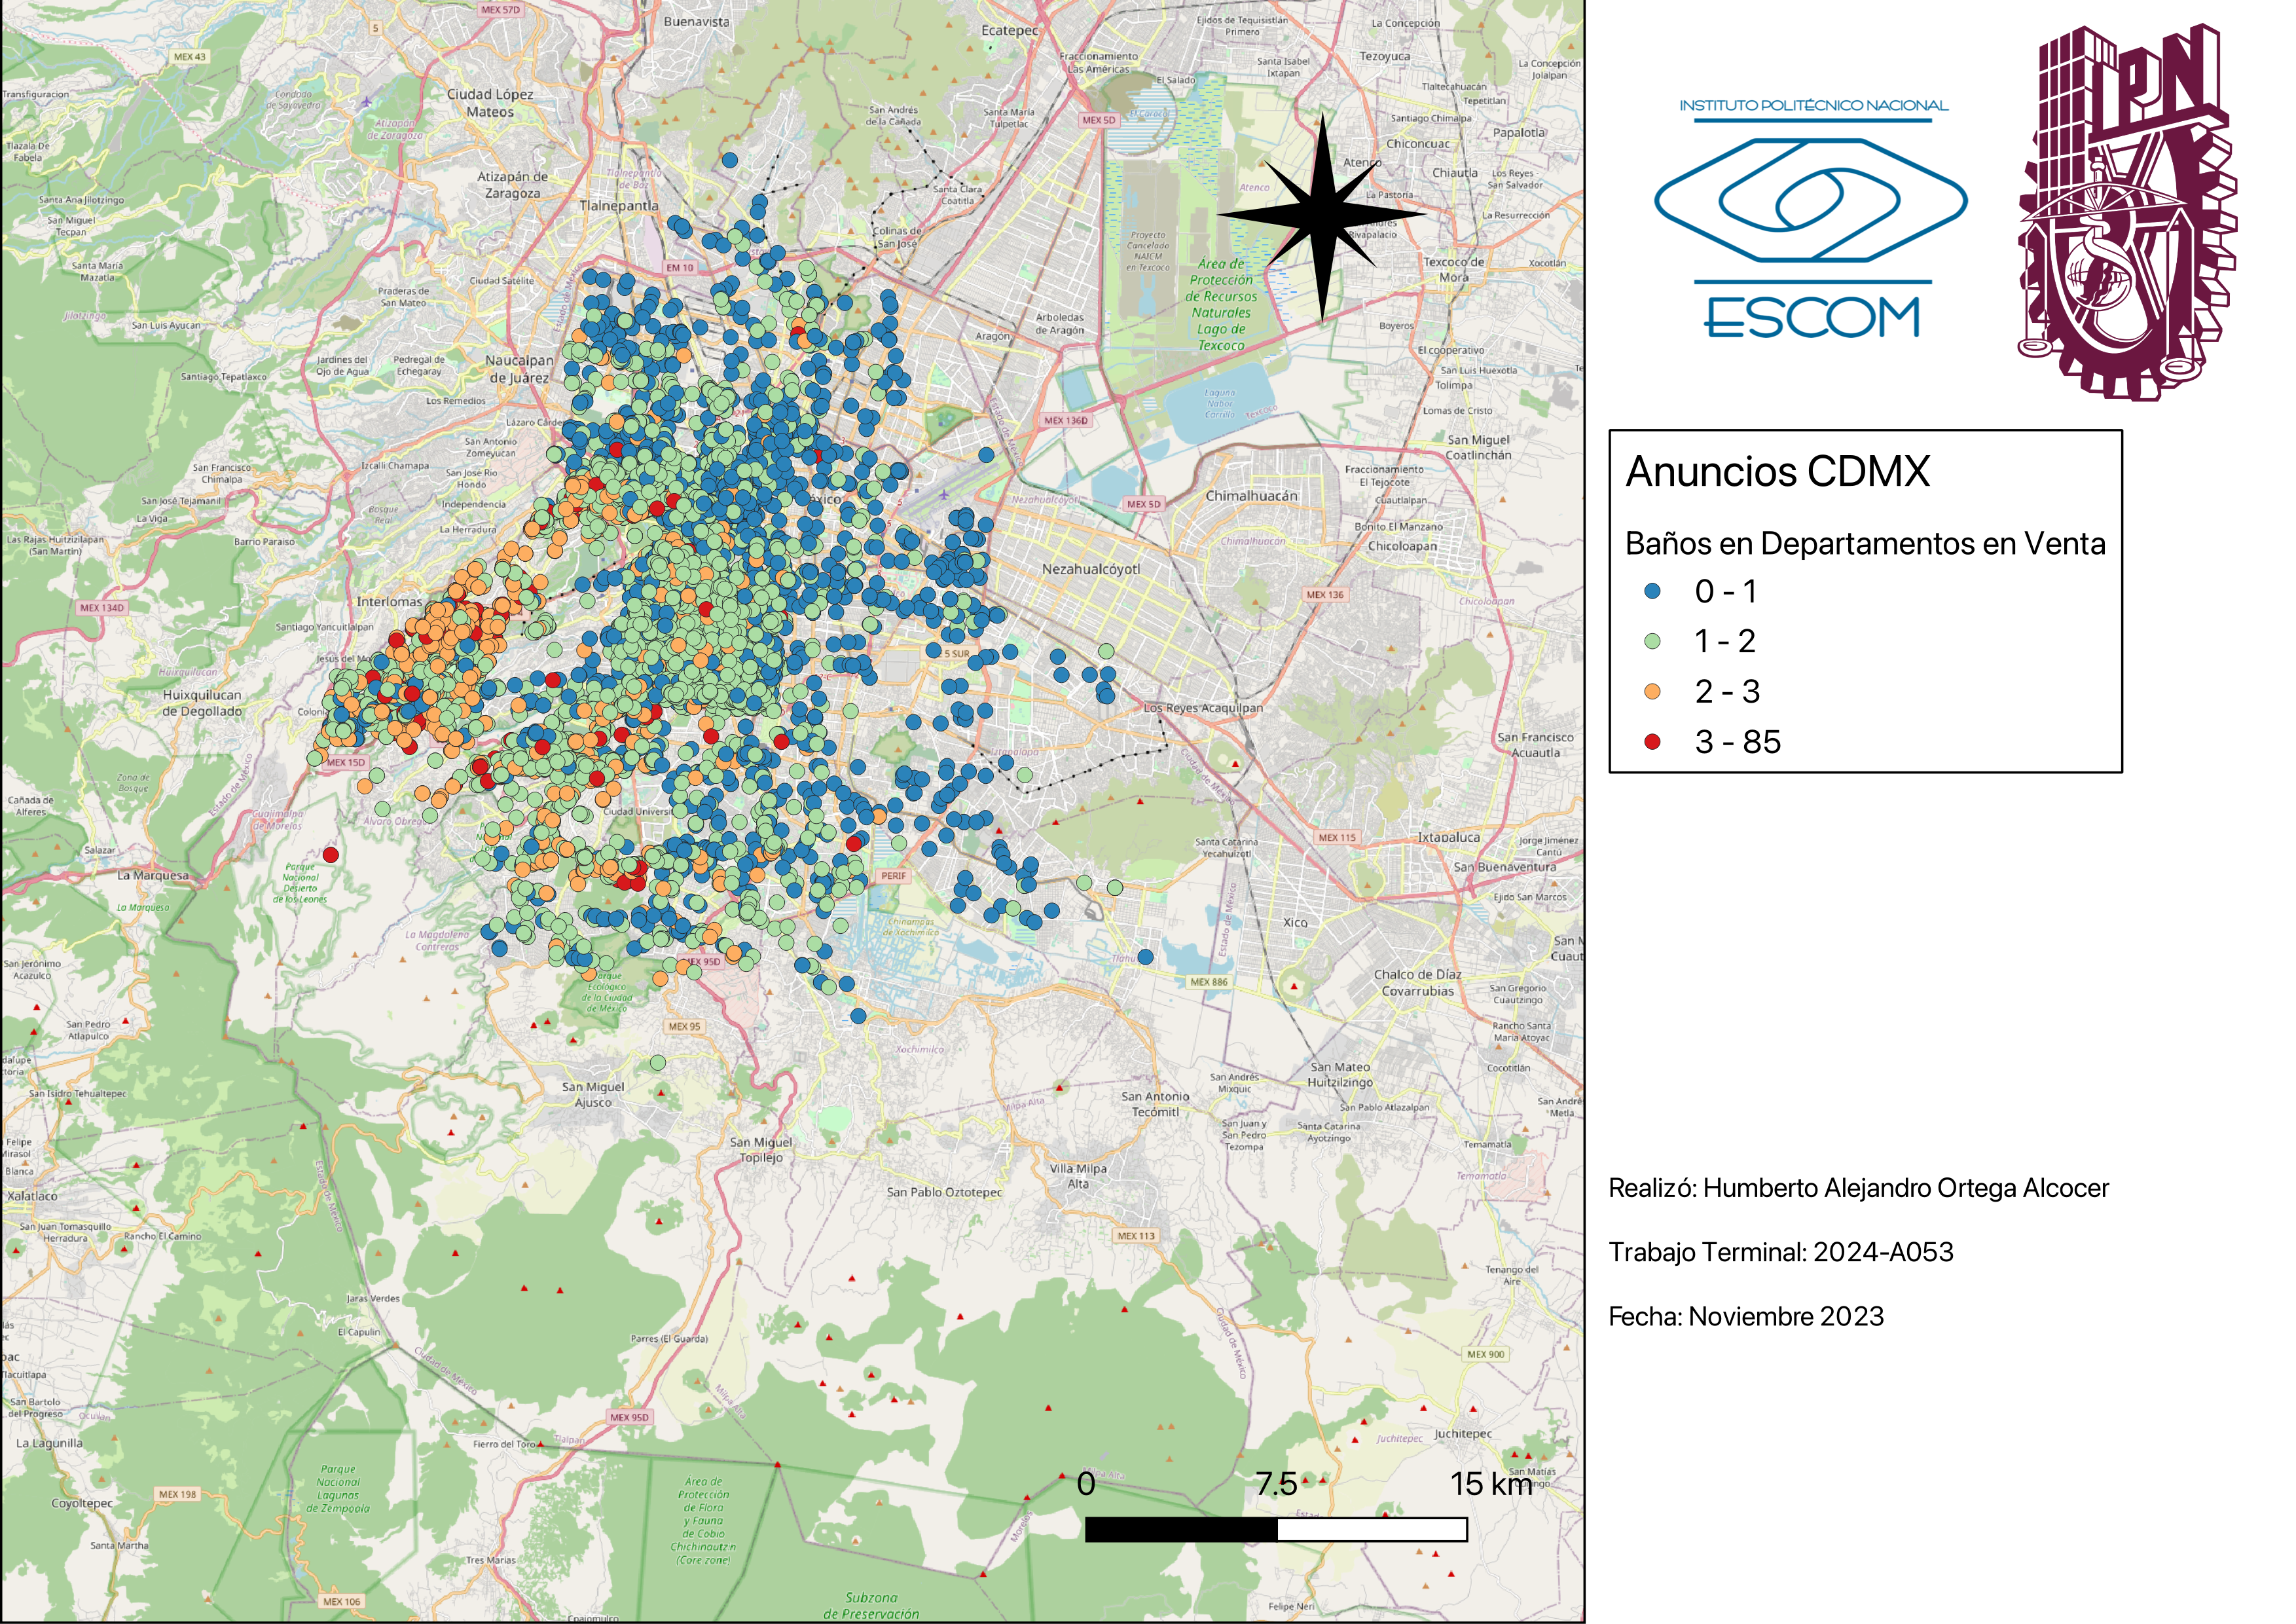
\includegraphics[width=0.9\textwidth]{imagenes/03-analisis/mapa-densidad-banos.png}
  \caption{Mapa de calor de número de baños.}
  \label{fig:mapa_calor_banos}
\end{figure}

De aquí, podemos derivar las siguientes conclusiones:

\begin{itemize}
  \item La gran mayoría de los departamentos en la Ciudad de México tienen 1 o
  2 baños.
  \item Los departamentos con 1 baño se encuentran en las zonas con mayor
  densidad de población, como la zona centro de la Ciudad de México.
  \item Los departamentos con 3 o más baños se encuentran en las zonas con
  mayor precio, como la zona poniene de la Ciudad de México.
\end{itemize}

\subsubsection{Mapa de calor de metros cuadrados}

La distribución de las superficies de departamentos en la Ciudad de México nos
permiten obtener un vistazo sobre la relación directa en el precio estimado
por metro cuadrado por zona, un factor determinante en el mercado inmobiliario.
En la Figura \ref{fig:mapa_calor_metros_cuadrados} se muestra el mapa de calor
de metros cuadrados para el conjunto de datos de bienes raíces.

\begin{figure}[H]
  \centering
  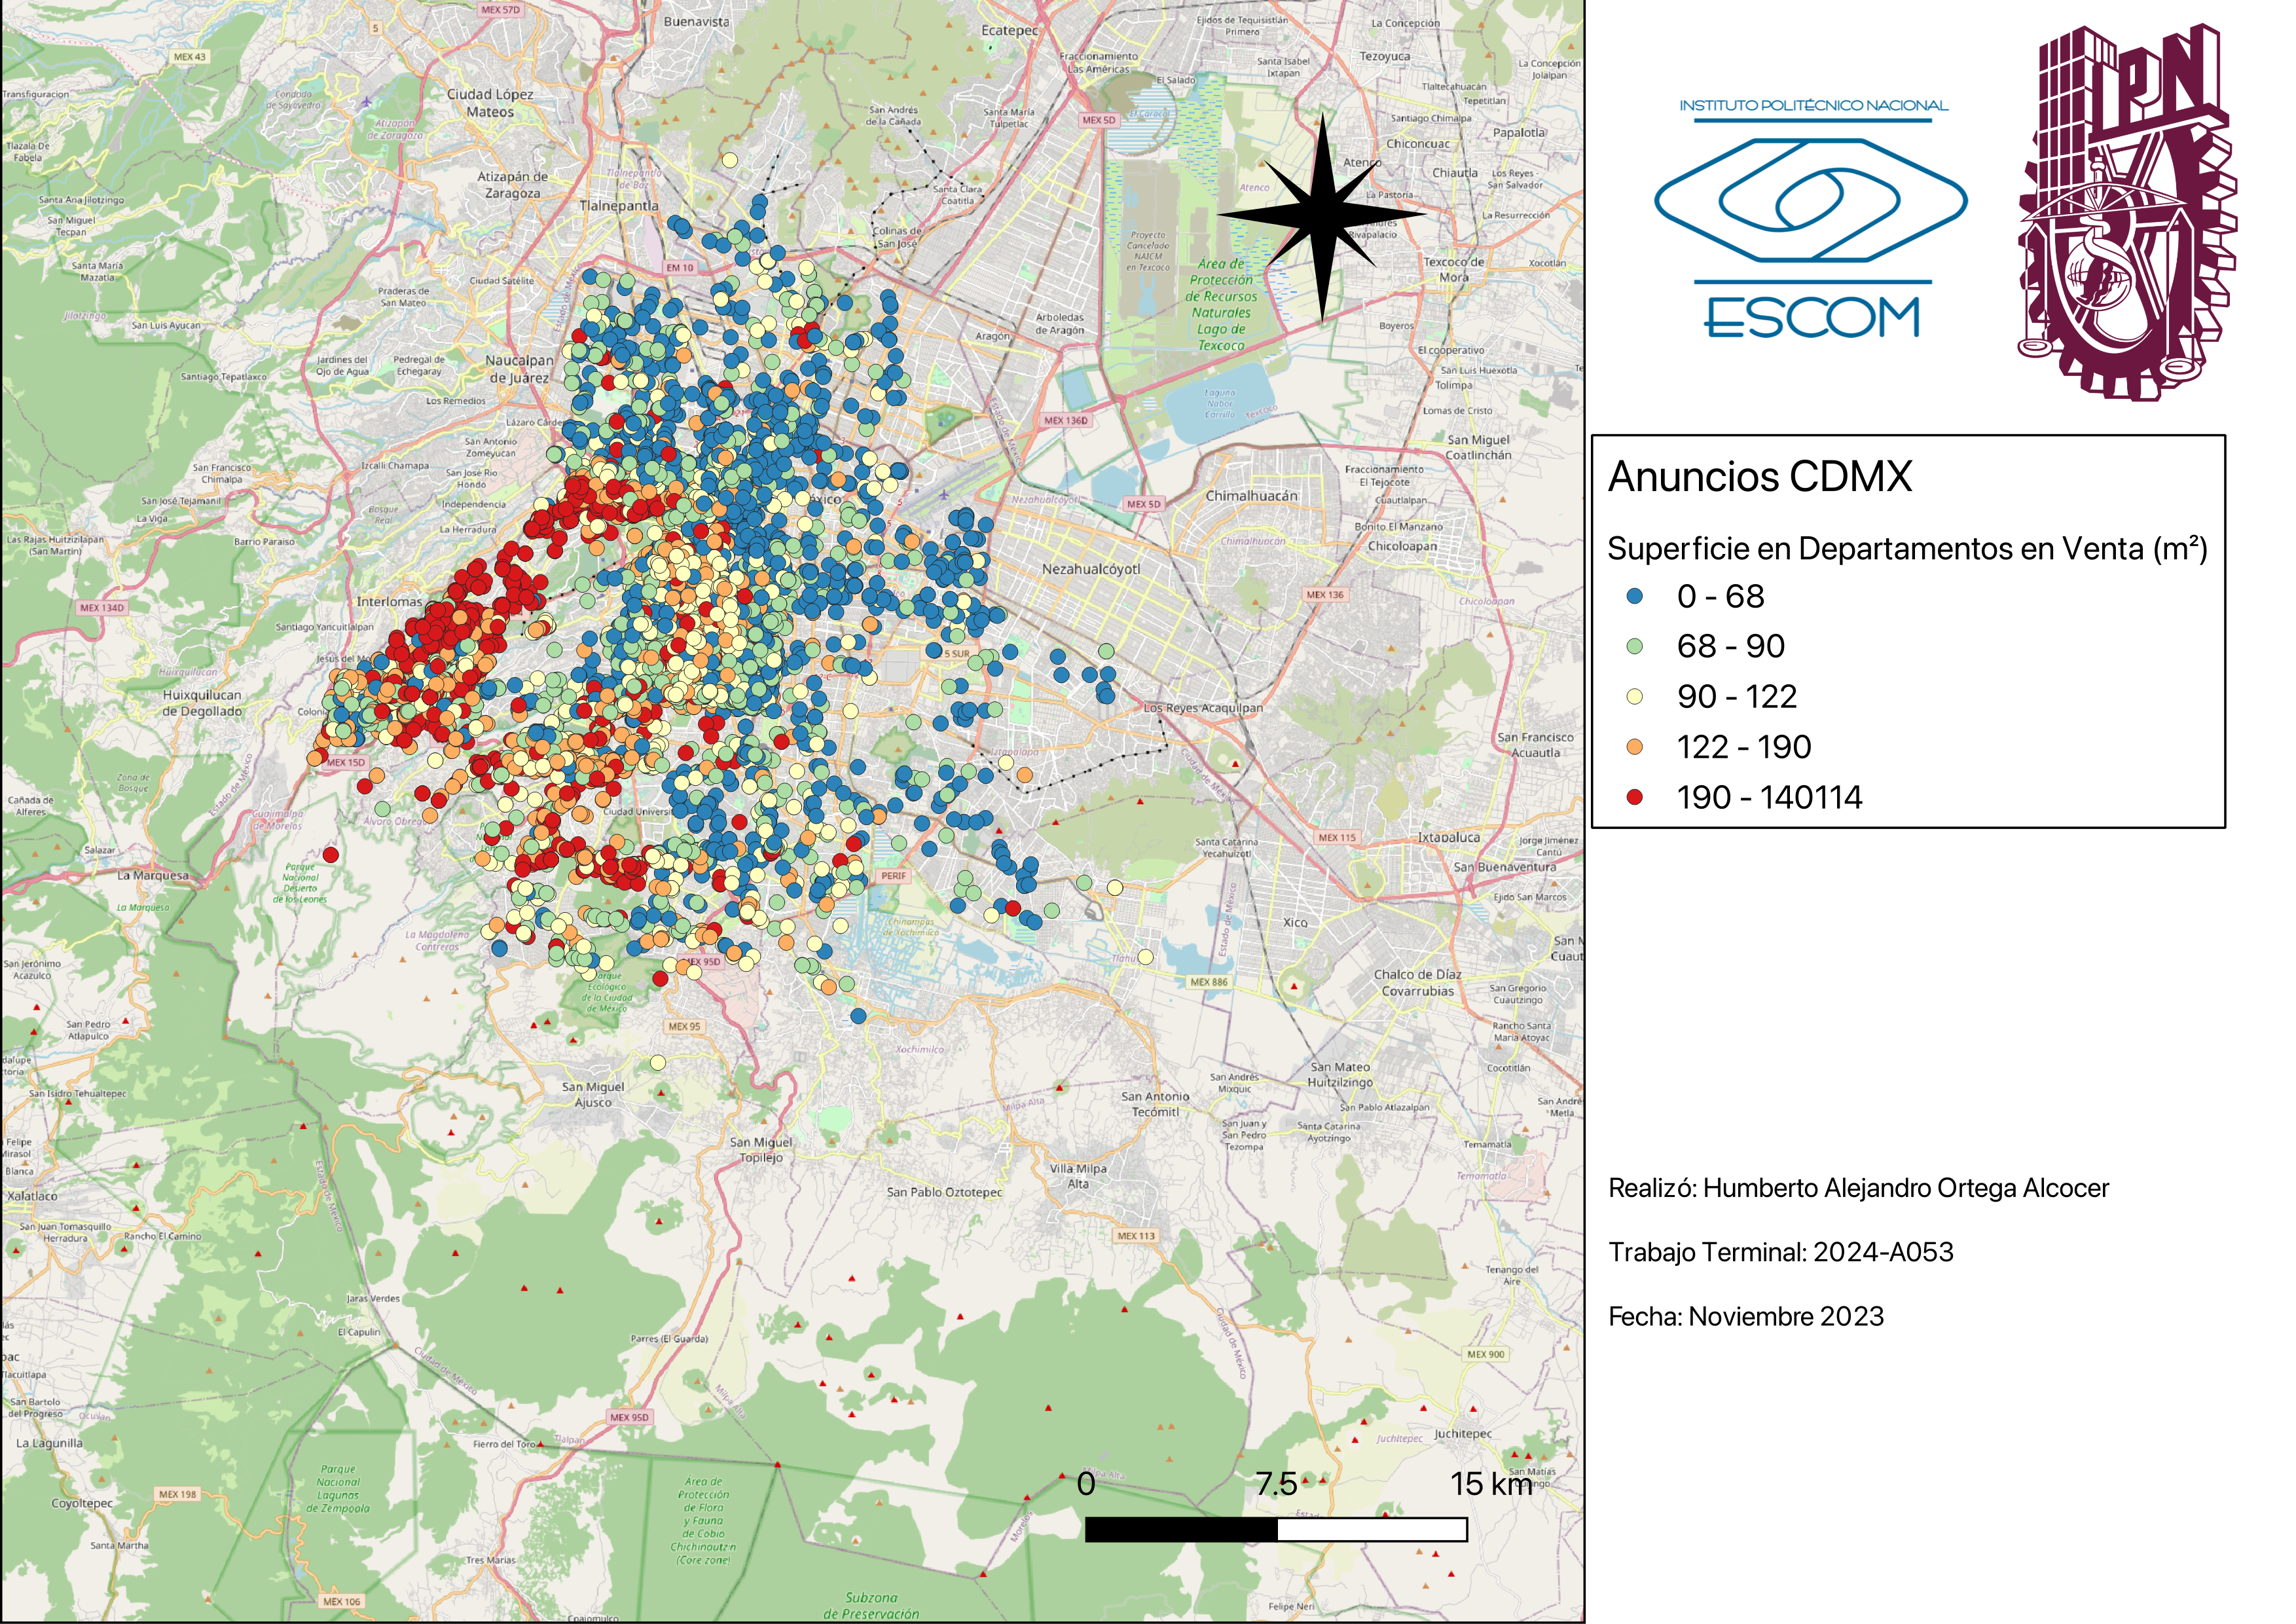
\includegraphics[width=0.9\textwidth]{imagenes/03-analisis/mapa-densidad-metros-cuadrados.png}
  \caption{Mapa de calor de metros cuadrados.}
  \label{fig:mapa_calor_metros_cuadrados}
\end{figure}

De aquí, podemos derivar las siguientes conclusiones:

\begin{itemize}
  \item La gran mayoría de los departamentos en la Ciudad de México tienen entre
  50 y 100 metros cuadrados.
  \item Los departamentos con menos de 50 metros cuadrados se encuentran en las
  zonas con mayor densidad de población, como la zona centro de la Ciudad de
  México. A su vez, estos departamentos tienen un precio por metro cuadrado más
  alto.
  \item Los departamentos con más de 100 metros cuadrados se encuentran en las
  zonas con mayor precio, como la zona poniene de la Ciudad de México.
\end{itemize}

\subsubsection{Mapa de calor de antigüedad}

La antigüedad de los departamentos es un factor determinante en el precio de los
mismos, ya que los departamentos más antiguos tienden a tener un precio más bajo
que los departamentos nuevos. Por otra parte, aunque no es el único factor a
considerar, al ser una zona sísmica, la antigüedad de los departamentos es un
factor importante a considerar para la seguridad de los habitantes. En la Figura
\ref{fig:mapa_calor_antiguedad} se muestra el mapa de calor de antigüedad para
el conjunto de datos de bienes raíces.

\begin{figure}[H]
  \centering
  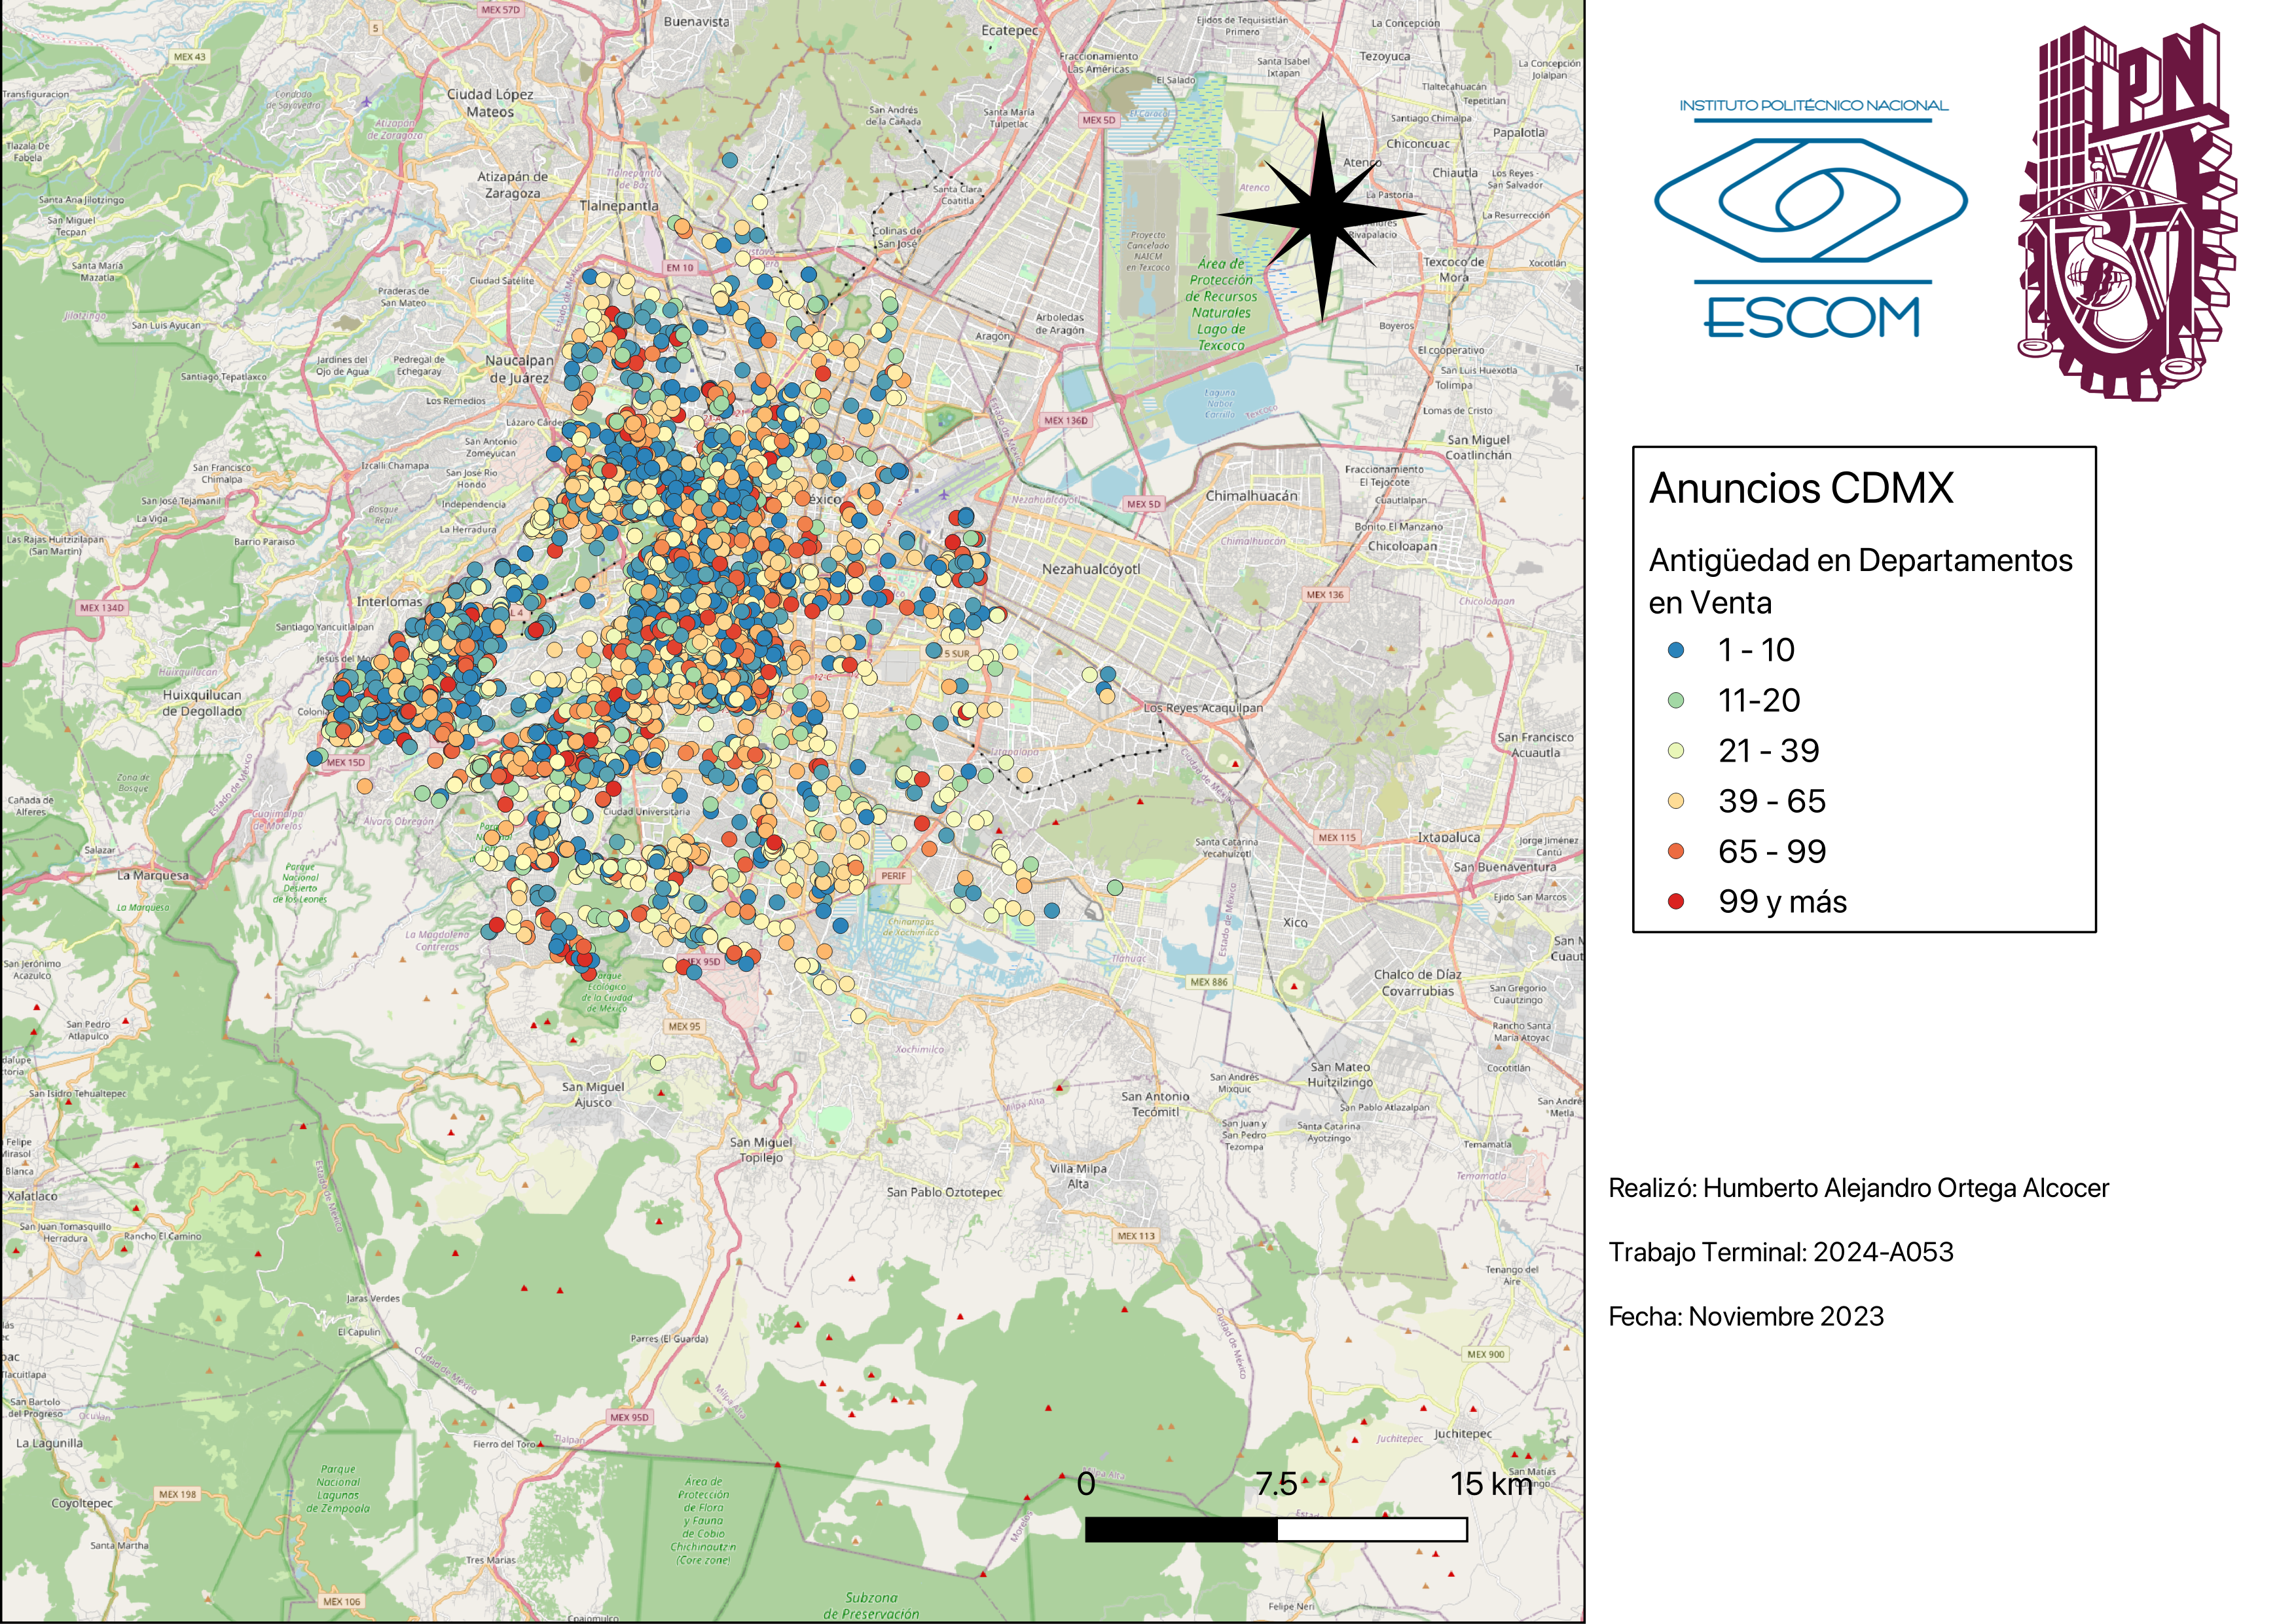
\includegraphics[width=0.9\textwidth]{imagenes/03-analisis/mapa-densidad-antiguedad.png}
  \caption{Mapa de calor de antigüedad.}
  \label{fig:mapa_calor_antiguedad}
\end{figure}

De aquí, podemos derivar las siguientes conclusiones:

\begin{itemize}
  \item La gran mayoría de los departamentos en la Ciudad de México tienen entre
  0 y 20 años de antigüedad.
  \item Los departamentos con menos de 20 años de antigüedad se encuentran en las
  zonas con mayor densidad de población, como la zona centro de la Ciudad de
  México. A su vez, estos departamentos tienen un precio más alto.
  \item Los departamentos con más de 20 años de antigüedad se encuentran en las
  zonas con mayor precio, como la zona poniene de la Ciudad de México.
\end{itemize}

\subsubsection{Mapa de calor por número de estacionamientos}

Los estacionamientos son un factor muy importante en la Ciudad de México, ya que
una gran cantidad de personas utilizan automóvil para transportarse. En la
Figura \ref{fig:mapa_calor_estacionamientos} se muestra el mapa de calor de
número de estacionamientos para el conjunto de datos de bienes raíces.

\begin{figure}[H]
  \centering
  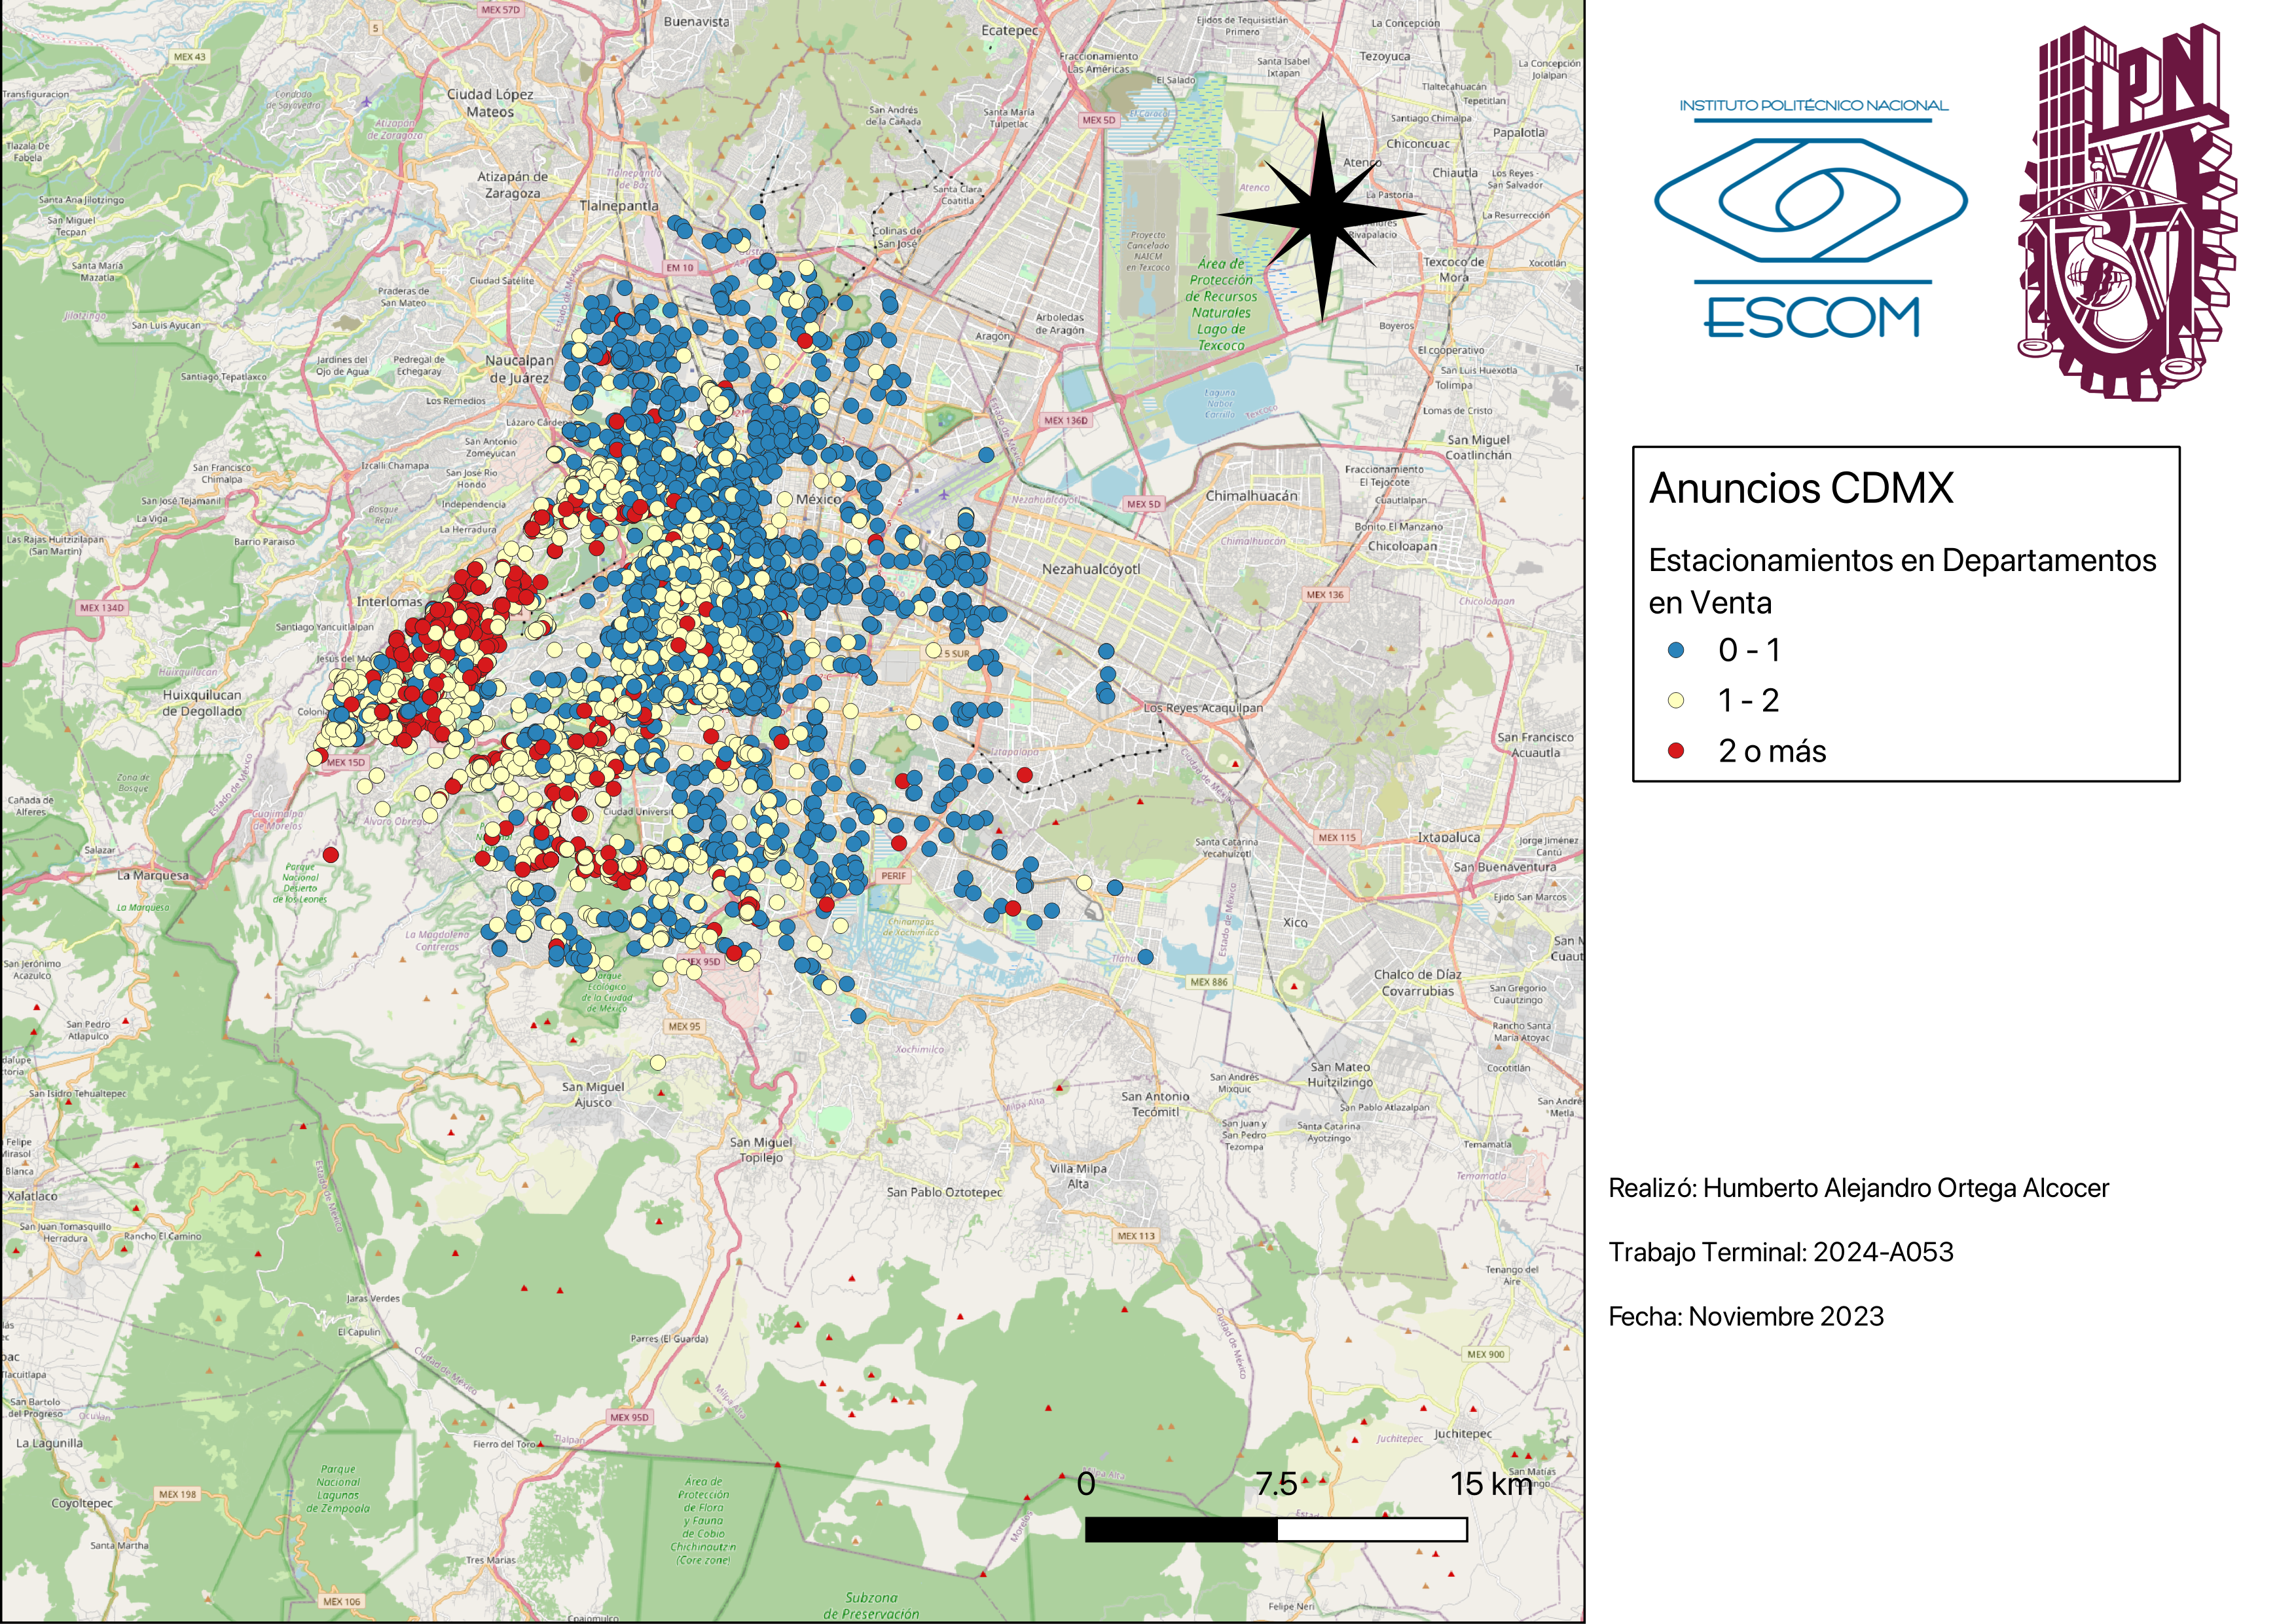
\includegraphics[width=0.9\textwidth]{imagenes/03-analisis/mapa-densidad-estacionamientos.png}
  \caption{Mapa de calor de número de estacionamientos.}
  \label{fig:mapa_calor_estacionamientos}
\end{figure}

De aquí, podemos derivar las siguientes conclusiones:

\begin{itemize}
  \item La gran mayoría de los departamentos en la Ciudad de México tienen 1 o
  2 estacionamientos.
  \item Los departamentos con 1 estacionamiento se encuentran en las zonas con
  mayor densidad de población, como la zona centro de la Ciudad de México.
  \item Los departamentos con 3 o más estacionamientos se encuentran en las
  zonas con mayor precio, como la zona poniene de la Ciudad de México.
\end{itemize}


\subsection{Análisis Exploratorio Econométrico}

La econometría es un campo de estudio que utiliza métodos estadísticos y
matemáticos para analizar y comprender las relaciones económicas, ayudando a
distinguir entre buenas y malas ideas en economía, negocios y políticas
públicas. Se enfoca en proporcionar respuestas cuantitativas a preguntas
importantes en estos ámbitos, permitiendo vislumbrar cómo individuos, empresas
y gobiernos toman decisiones basadas en dichas relaciones. La econometría busca
hacer la teoría inmediatamente relevante para las aplicaciones prácticas,
integrando la teoría y las aplicaciones para hacer el aprendizaje más atractivo
y pertinente \cite{stock2012introduccion}.

El análisis exploratorio econométrico consiste en caracterizar, mediante el uso
de estadísticas descriptivas, las variables que se utilizarán para el
entrenamiento del modelo de aprendizaje automático.

\begin{itemize}
  \item Análisis descriptivo
  \item Correlación entre variables
  \item Análisis de regresión simple y múltiple
  \item Análisis de componentes principales (PCA)
\end{itemize}

\subsubsection{Análisis Descriptivo}

Un análisis descriptivo nos permite caracterizar las variables que se utilizarán
para el entrenamiento del modelo de aprendizaje automático. Además, nos permite
obtener información rápida sobre nuestros datos a bien de poder determinar si
los datos son adecuados para el entrenamiento del modelo.

Para realizar un análisis descriptivo, se utilizó la librería Pandas de Python,
la cual permite realizar análisis descriptivos de manera sencilla. En el Código
\ref{lst:analisis_descriptivo} se muestra el código utilizado para realizar el
análisis descriptivo.

\begin{lstlisting}[language=Python, label=lst:analisis_descriptivo, caption=Análisis descriptivo.]
import pandas as pd

# Carga de datos
df = pd.read_csv('scrape-20231103-16-27-14.csv')

# Columnas a analizar
numeric_columns = ['Price', 'Size_Terrain', 'Size_Construction',
                   'Rooms', 'Bathrooms', 'Parking', 'Age']

# Seleccionar solo las columnas numéricas
df_numeric = df[numeric_columns]

# Analisis descriptivo
resultado = df_numeric.describe(include='all')

# Imprimir resultado
print(resultado)
\end{lstlisting}

En el Cuadro \ref{table:analisis_descriptivo} se muestran los resultados del
análisis descriptivo.

\begin{table}[h!]
\centering
\caption{Estadísticas Descriptivas de los Listados de Bienes Raíces}
\label{table:analisis_descriptivo}
\sisetup{
  round-mode          = places, % Rounds numbers
  round-precision     = 2, % to 2 places
}
\tiny % Makes the font smaller; use \scriptsize or \tiny for even smaller sizes
\begin{tabular}{
  l
  S[table-format=2.2]
  S[table-format=5.0]
  S[table-format=5.0]
  S[table-format=2.0]
  S[table-format=2.0]
  S[table-format=1.0]
  S[table-format=3.0]
}
\toprule
  {} & {Precio (MDP)} & {Superficie} & {Superficie Cons.} & {Recámaras} & {Baños} & {Estacionamiento} & {Antigüedad} \\
\midrule
count & 17.876 & 17740 & 17694 & 17537 & 17478 & 16269 & 10758 \\
mean  & 12.18 & 181 & 156 & 2 & 2 & 2 & 15 \\
std   & 183.45 & 1601 & 426 & 1 & 1 & 1 & 15 \\
min   & 0.0015 & 1 & 1 & 1 & 1 & 1 & 1 \\
25\%  & 3.58 & 75 & 75 & 2 & 2 & 1 & 5 \\
50\%  & 5.65 & 109 & 107 & 2 & 2 & 2 & 10 \\
75\%  & 9.95 & 180 & 179 & 3 & 2 & 2 & 20 \\
max   & 175 & 1401 & 3301 & 6 & 5 & 8 & 310 \\
\bottomrule
\end{tabular}
\normalsize % Resets the font size to normal
\end{table}

De aquí, podemos derivar las siguientes conclusiones:

\begin{itemize}
  \item El precio promedio de las propiedades es de 12.18 millones de pesos, con una amplia variación indicada por una desviación estándar de 183.45 millones de pesos.
  \item La superficie del terreno varía significativamente entre las propiedades, con un promedio de 181 \(m^2\) y una desviación estándar alta de 1601 \(m^2\).
  \item La superficie de construcción promedio es de 155 \(m^2\), con propiedades que van desde 1 \(m^2\) hasta 33015 \(m^2\).
  \item El número promedio de habitaciones por propiedad es de aproximadamente 2.34, con la mayoría de las propiedades teniendo entre 2 y 3 habitaciones.
  \item El número de baños y espacios de estacionamiento también varía, con un promedio cercano a 2 para cada uno.
  \item La edad media de las propiedades es de aproximadamente 14.78 años, con algunas propiedades teniendo hasta 310 años de antigüedad.
  \item Los mínimos en varias categorías (como 1 \(m^2\) de superficie de construcción) podrían indicar datos atípicos o errores en los datos.
\end{itemize}

\subsubsection{Correlación entre variables}

La correlación entre variables nos permite determinar si existe una relación
entre las variables que se utilizarán para el entrenamiento del modelo de
aprendizaje automático. Este análisis es importante ya que nos permite determinar
los pesos que podrían tener las variables en el entrenamiento del modelo. Por
otra parte, entender qué variables tienen más impacto en otras nos permite
determinar si es necesario realizar un análisis de regresión simple o múltiple.

Para realizar un análisis de correlación entre variables, se utilizó la librería
Pandas de Python, la cual permite realizar análisis de correlación entre variables
de manera sencilla. En el Código \ref{lst:correlacion_variables} se muestra el
código utilizado para realizar el análisis de correlación entre variables.

\begin{lstlisting}[language=Python, label=lst:correlacion_variables, caption=Correlación entre variables.]
import pandas as pd

# Carga de datos
df = pd.read_csv('scrape-20231103-16-27-14.csv')

# Columnas a analizar
numeric_columns = ['Price', 'Size_Terrain', 'Size_Construction',
                   'Rooms', 'Bathrooms', 'Parking', 'Age']

# Seleccionar solo columnas numéricas
df_numeric = df[numeric_columns]

# Correlación de Pearson
resultado = df_numeric.corr(method='pearson')

# Imprimir resultado
print(resultado)
\end{lstlisting}

En el Cuadro \ref{table:correlacion_variables} se muestran los resultados del
análisis de correlación entre variables.

\begin{table}[h!]
\centering
\caption{Matriz de Correlación entre Variables}
\label{table:correlacion_variables}
\sisetup{
  round-mode          = places, % Rounds numbers
  round-precision     = 2, % to 2 places
}
\tiny % Makes the font smaller; use \scriptsize or \tiny for even smaller sizes
\begin{tabular}{
  l
  S[table-format=1.2]
  S[table-format=1.2]
  S[table-format=1.2]
  S[table-format=1.2]
  S[table-format=1.2]
  S[table-format=1.2]
  S[table-format=1.2]
}
\toprule
  {} & {Precio} & {Superficie} & {Superficie Cons.} & {Recámaras} & {Baños} & {Estacionamiento} & {Antigüedad} \\
\midrule
Precio              & 1.00 & 0.00 & 0.01 & 0.02 & 0.02 & 0.02 & 0.01 \\
Superficie          & 0.00 & 1.00 & 0.27 & 0.04 & 0.04 & 0.06 & -0.01 \\
Superficie Cons.    & 0.01 & 0.27 & 1.00 & 0.15 & 0.14 & 0.21 & 0.01 \\
Recámaras           & 0.02 & 0.04 & 0.15 & 1.00 & 0.47 & 0.46 & 0.13 \\
Baños               & 0.02 & 0.04 & 0.14 & 0.47 & 1.00 & 0.46 & -0.05 \\
Estacionamiento     & 0.02 & 0.06 & 0.21 & 0.46 & 0.46 & 1.00 & -0.10 \\
Antigüedad          & 0.01 & -0.01 & 0.01 & 0.13 & -0.05 & -0.10 & 1.00 \\
\bottomrule
\end{tabular}
\normalsize % Resets the font size to normal
\end{table}

De aquí, podemos derivar las siguientes conclusiones:

\begin{itemize}
  \item \textbf{Relaciones Débiles}: Los coeficientes de correlación entre el precio y las demás
variables son muy bajos (todos inferiores a 0.03), lo que sugiere que no hay una
relación lineal fuerte entre el precio y las otras características de las
propiedades en el conjunto de datos.
\item \textbf{Superficie y Construcción}: La correlación más fuerte observada es entre la superficie
del terreno y la superficie construida (0.27), lo cual es esperable ya que propiedades
con terrenos más grandes tienden a tener mayores construcciones.
\item \textbf{Recámaras y Baños/Estacionamiento}: Hay una correlación moderada entre el número
de recámaras y baños (0.47) y recámaras y estacionamientos (0.46), lo que indica
que propiedades con más recámaras tienden a tener más baños y más espacio de
estacionamiento.
\item \textbf{Edad de la Propiedad}: La edad tiene una correlación negativa con el estacionamiento
y los baños, aunque es débil. Esto podría sugerir que las propiedades más antiguas
tienen menos baños y menos estacionamientos, pero es una relación muy leve.
\item \textbf{Relevancia para IA}: Para la valuación inmobiliaria con IA utilizando redes
neuronales, estos resultados implican que las variables incluidas no proporcionan
una indicación clara del precio de manera individual. Por lo tanto, el modelo
de red neuronal deberá capturar relaciones no lineales complejas o interacciones
entre variables que no son evidentes a partir de los coeficientes de correlación
lineal.
\end{itemize}

\subsubsection{Análisis de regresión simple y múltiple}

Con el fin de poder determinar la relación entre las variables que se utilizarán
para el entrenamiento del modelo de aprendizaje automático, se realizó un análisis
de regresión simple y múltiple. Las regresiones simples y múltiples son técnicas
estadísticas que permiten determinar la relación entre una variable dependiente
y una o más variables independientes. En el caso de la regresión simple, se
determina la relación entre una variable dependiente y una variable independiente,
mientras que en el caso de la regresión múltiple, se determina la relación entre
una variable dependiente y dos o más variables independientes \cite{stock2012introduccion}.

Para realizar un análisis de regresión simple y múltiple, se utilizó la librería
StatsModels de Python, la cual permite realizar análisis de regresión simple y
múltiple de manera sencilla. En el Código \ref{lst:regresion_simple_multiple} se
muestra el código utilizado para realizar el análisis de regresión simple y múltiple.

\begin{lstlisting}[language=Python, label=lst:regresion_simple_multiple, caption=Regresión simple y múltiple.]
import statsmodels.api as sm
import pandas as pd
import numpy as np

# Carga de datos
df = pd.read_csv('scrape-20231103-16-27-14.csv')

# Reemplazar infinitos con NaN
df.replace([np.inf, -np.inf], np.nan, inplace=True)

# Eliminar filas con valores NaN
df_clean = df.dropna(subset=['Price','Size_Terrain', 'Size_Construction',
                             'Rooms', 'Bathrooms', 'Parking'])

# Columnas a analizar
numeric_columns = ['Price', 'Size_Terrain', 'Size_Construction',
                   'Rooms', 'Bathrooms', 'Parking', 'Age']

# Seleccionar solamente columnas numéricas
df_numeric = df_clean[numeric_columns]

# Regresión simple usando Size_Construction como predictor del Price
X_simple = sm.add_constant(df_numeric['Size_Construction']) # Añadir constante
modelo_simple = sm.OLS(df_numeric['Price'], X_simple).fit()

# Regresión múltiple usando Size_Construction, Rooms, Bathrooms y Parking como predictores del Price
X_multiple = sm.add_constant(df_numeric[['Size_Terrain', 'Rooms', 'Bathrooms', 'Parking']]) # Añadir constante
modelo_multiple = sm.OLS(df_numeric['Price'], X_multiple).fit()

# Imprimir los resultados
print("Regresión simple")
print(modelo_simple.summary())
print()
print("Regresión múltiple")
print(modelo_multiple.summary())
\end{lstlisting}

En el Cuadro \ref{table:regresion_simple} se muestran los resultados del análisis
de regresión simple.

\begin{table}[ht!]
\centering
\caption{Resultados de la Regresión Simple}
\label{table:regresion_simple}
\begin{tabular}{
  l
  S[table-format=-1.4]
  S[table-format=1.4]
}
\toprule
{Variable} & {Coeficiente} & {Error Estándar} \\
\midrule
Constante              & 1.21e+07 & 1.69e+06 \\
Size\_Construction & 4917.3102 & 4216.805 \\
\bottomrule
\end{tabular}
\end{table}

\textit{Nota:} R-cuadrado: 0.000; F-estadístico: 1.360, P-valor: 0.244. El Omnibus y Jarque-Bera indican una distribución no normal de los residuos.

En el Cuadro \ref{table:regresion_multiple} se muestran los resultados del análisis
de regresión múltiple.

\begin{table}[h!]
\centering
\caption{Resultados de la Regresión Múltiple}
\label{table:regresion_multiple}
\begin{tabular}{
  l
  S[table-format=-1.4]
  S[table-format=1.4]
}
\toprule
{Variable} & {Coeficiente} & {Error Estándar} \\
\midrule
Constante         & -6.191e+04 & 5.63e+06 \\
Size\_Terrain     & 76.1953    & 925.533 \\
Rooms             & 1.772e+06  & 2.6e+06 \\
Bathrooms         & 1.304e+06  & 1.8e+06 \\
Parking           & 3.122e+06  & 2.03e+06 \\
\bottomrule
\end{tabular}
\end{table}

\textit{Nota:} R-cuadrado: 0.001; F-estadístico: 2.021, P-valor: 0.0887. Las notas adicionales mencionan errores estándar que asumen que la matriz de covarianza de los errores está correctamente especificada y un número de condición grande, lo que podría indicar multicolinealidad.

De los resultados obtenidos, podemos derivar las siguientes conclusiones:

\begin{itemize}
  \item Para la regresión simple, el R-cuadrado es 0, lo que indica que el modelo
    no explica nada de la variabilidad del precio. Esto está reforzado por el alto
    P-valor, sugiriendo que la variable Size\_Construction no es un predictor
    estadísticamente significativo del precio.
  \item Para la regresión múltiple, aunque incluye más variables, el R-cuadrado
    sigue siendo muy bajo (0.001), indicando que el modelo explica menos del 0.1\%
    de la variabilidad del precio. Los P-valores también son altos, sugiriendo
    que ninguna de las variables independientes es un predictor significativo
    del precio.
  \item Las altas estadísticas de Omnibus y Jarque-Bera junto con la significativa
    desviación (skewness) y la kurtosis apuntan a una distribución no normal de los
    residuos, lo que podría afectar la fiabilidad de los tests estadísticos.
  \item El número de condición alto en la regresión múltiple sugiere que podría
    haber problemas de multicolinealidad en el modelo, lo que significa que
    algunas de las variables independientes están correlacionadas entre sí.
\end{itemize}

\subsubsection{Análisis de componentes principales (PCA)}

El análisis de componentes principales es un método estadístico versátil para
reducir una tabla de datos de casos por variables a sus características esenciales,
llamadas componentes principales. Los componentes principales son unas pocas
combinaciones lineales de las variables originales que explican de manera
máxima la varianza de todas las variables. En el proceso, el método proporciona
una aproximación de la tabla de datos original utilizando solo estos pocos
componentes principales \cite{greenacre2022principal}.

Para poder llevar a cabo este análisis, se utilizó la librería Scikit-Learn de
Python, la cual permite realizar análisis de componentes principales de manera
sencilla. En el Código \ref{lst:pca} se muestra el código utilizado para realizar
el análisis de componentes principales.

\begin{lstlisting}[language=Python, label=lst:pca, caption=Análisis de componentes principales (PCA).]
import pandas as pd
import numpy as np
from sklearn.decomposition import PCA
from sklearn.preprocessing import StandardScaler

# Carga de datos
df = pd.read_csv('scrape-20231103-16-27-14.csv')

# Reemplazar infinitos con NaN
df.replace([np.inf, -np.inf], np.nan, inplace=True)

# Eliminar filas con valores NaN
df_clean = df.dropna(subset=['Price','Size_Terrain', 'Size_Construction',
                             'Rooms', 'Bathrooms', 'Parking', 'Age'])

# Columnas a analizar
numeric_columns = ['Price', 'Size_Terrain', 'Size_Construction',
                   'Rooms', 'Bathrooms', 'Parking', 'Age']

# Seleccionar únicamente las columnas numéricas
df_numeric = df_clean[numeric_columns]

# Estandarizar los datos
scaler = StandardScaler()
df_scaled = scaler.fit_transform(df_numeric)

# PCA
pca = PCA(n_components=2) # Reducir a 2 componentes principales

componentes_principales = pca.fit_transform(df_scaled)

# Imprimir los componentes principales
print('Componentes principales')
print(componentes_principales)

# Varianza explicada
print('Varianza explicada')
print(pca.explained_variance_ratio_)

# Coeficientes de los componentes
print('Coeficientes de los componentes')
print(pca.components_)


\end{lstlisting}

Los resultados del análisis de componentes principales se muestran en el Cuadro
\ref{table:pca-results}.

\begin{table}[h]
\small
\centering
\begin{tabular}{|c|c|c|}
\hline
\rowcolor{azulclaro}
  \textbf{Componente} & \textbf{Varianza Explicada} & \textbf{Coeficientes} \\ \hline
1 & 30.61\% & [0.047, 0.083, 0.458, 0.505, 0.485, 0.537, 0.051] \\ \hline
2 & 15.42\% & [0.185, -0.094, 0.008, 0.255, -0.109, -0.237, 0.908] \\ \hline
\end{tabular}
\caption{Resultados del Análisis de Componentes Principales}
\label{table:pca-results}
\end{table}

En la figura \ref{fig:pca} se muestra la visualización de los componentes
principales.

\begin{figure}[H]
  \centering
  \includegraphics[width=0.8\textwidth]{imagenes/03-analisis/analisis-econometrico/analisis-pca.png}
  \caption{Visualización de los componentes principales.}
  \label{fig:pca}
\end{figure}

De los resultados obtenidos, podemos derivar las siguientes conclusiones:

\begin{enumerate}
    \item Las características físicas de los inmuebles, como el tamaño de la construcción, el número de habitaciones, baños y estacionamientos, son las que más varían y tienen mayor influencia en el primer componente principal.
    \item La edad del inmueble es una dimensión importante de variabilidad y es el factor predominante en el segundo componente principal.
    \item Estos dos componentes capturan casi la mitad de la variabilidad total de los datos, lo que indica una distribución equilibrada de la influencia de las diferentes variables.
    \item Se recomienda visualizar estos componentes principales en un gráfico bidimensional para identificar patrones o agrupaciones interesantes en los datos.
    \item Dependiendo de los objetivos del análisis, podría ser útil considerar aumentar el número de componentes principales para capturar más variabilidad.
\end{enumerate}

\section{Algoritmos de Aprendizaje Automático}

Para la realización de este proyecto se deberán considerar múltiples algoritmos
de aprendizaje automático, los cuales se utilizarán para el entrenamiento de los
modelos de valuación inmobiliaria. Estos algoritmos serán utilizados para realizar
una comparativa entre el rendimiento y ajuste de cada uno con el objetivo de
poder determinar, una vez finalizada la creación del conjunto de datos final,
cuál algoritmo emplear para la creación del modelo de valuación inmobiliaria final.

\subsection{Máquinas de Soporte Vectorial}

Método efectivo en espacios de alta dimensión. Utiliza hiperplanos para separar
clases de datos. Los hiperplanos se eligen maximizando el margen entre las clases.
Las SVMs pueden usar diferentes tipos de kernels, como lineal, polinomial y
radial, para adaptarse a la naturaleza no lineal de algunos datos \cite{10.1145/1143844.1143865}.

\subsection{Random Forest}

El algoritmo de bosques aleatorios, propuesto por L. Breiman en 2001, ha
sido extremadamente exitoso como un método de clasificación y regresión de propósito
general. El enfoque, que combina varios árboles de decisión aleatorizados y
agrega sus predicciones mediante promedios, ha mostrado
un excelente rendimiento en entornos donde el número de variables es
mucho mayor que el número de observaciones. Además, es lo suficientemente versátil
como para ser aplicado a problemas a gran escala, se adapta fácilmente a
varias tareas de aprendizaje ad hoc y devuelve medidas de la importancia de las variables
\cite{biau2016random}.

\subsection{Redes Neuronales Artificiales}

Las redes neuronales son un modelo de aprendizaje automático inspirado en el
funcionamiento del cerebro humano. Las redes neuronales se componen de neuronas
artificiales que se conectan entre sí para formar una red. Cada neurona artificial
tiene una o más entradas y una salida. Las entradas de una neurona artificial
están conectadas a otras neuronas artificiales a través de conexiones llamadas
pesos. Cada conexión tiene un peso asociado con él. El peso de una conexión
determina la influencia de una neurona en otra. Las neuronas artificiales
utilizan una función de activación para determinar su salida en función de sus
entradas y pesos. Las redes neuronales se utilizan para resolver problemas de
clasificación y regresión \cite{muller1995neural}.

\section{Estudio de Factibilidad}

Para poder determinar si el proyecto es factible, se realizó un estudio de
factibilidad, el cual se divide en tres partes: factibilidad técnica, factibilidad
económica y factibilidad operativa.

El objetivo general será determinar si el planteamiento del proyecto es viable
y si se puede llevar a cabo con los recursos disponibles.

\subsection{Factibilidad Técnica}

En el apartado de factibilidad técnica se analizaron los recursos técnicos
necesarios para poder llevar a cabo el proyecto planteado en el presente
documento. En el Cuadro \ref{table:factibilidad_tecnica} se muestra el análisis
de factibilidad técnica.

\begin{table}[H]
\centering
\begin{tabular}{|p{5cm}|c|c|}
\hline
\rowcolor{azulclaro}
  \centering\textbf{Recurso} & \centering\textbf{Disponibilidad}\arraybackslash & \centering\textbf{Viabilidad}\arraybackslash \\
\hline
Equipo de cómputo & Sí & Sí \\
\hline
  Software & Sí & Sí \\
\hline
  Conexión a internet & Sí & Sí \\
\hline
  Plataforma en la nube & Sí & Sí \\
\hline
\end{tabular}
\caption{Factibilidad Técnica}
\label{table:factibilidad_tecnica}
\end{table}

Dado que todos los recursos necesarios para llevar a cabo el proyecto se
encuentran disponibles, se puede concluir que el proyecto es factible desde el
punto de vista técnico.

\subsection{Factibilidad Económica}

Para llevar a cabo el proyecto será necesario contar con un presupuesto, el cual
se utilizará para la adquisición de recursos necesarios para el desarrollo del
mismo. En el Cuadro \ref{table:factibilidad_economica} se muestra el análisis de
factibilidad económica.

\begin{table}[H]
\centering
\begin{tabular}{|p{5cm}|c|c|}
\hline
\rowcolor{azulclaro}
  \centering\textbf{Recurso} & \textbf{Costo} & \textbf{Viabilidad}\arraybackslash \\
\hline
AWS & \$ 10 USD/mes & Sí \\
\hline
Equipo de cómputo & \$ 20,000.00 & Sí \\
\hline
  Recursos Humanos & \$ 15,000.00/mes & Sí \\
\hline
\end{tabular}
\caption{Factibilidad Económica}
\label{table:factibilidad_economica}
\end{table}

\textit{*Nota:} AWS ofrece un plan gratuito que incluye 750 horas de uso de instancias EC2
t2.micro, 5 GB de almacenamiento EBS, 40 GB de almacenamiento EFS, 750 horas de
uso de RDS, 25 horas de uso de DynamoDB, 15 GB de ancho de banda de salida, 1
millón de solicitudes de Lambda y 1 millón de solicitudes de API Gateway al mes
durante un año \cite{aws_free_2023}. A pesar de esto, se incluyó el costo de AWS
en el análisis de factibilidad económica para poder tener un presupuesto más realista
e inclusive realizar las proyecciones pertinentes en caso de que se requiera
utilizar recursos adicionales a los ofrecidos en el plan gratuito.

Debido a que se estiman 6 meses de trabajo, los costos finales del proyecto
se observan en el Cuadro \ref{table:costos_proyecto}.

\begin{table}[H]
\centering
\begin{tabular}{|c|p{5cm}|}
\hline
\rowcolor{azulclaro}
  \textbf{Recurso} & \centering\textbf{Costo}\arraybackslash \\
\hline
  AWS & \$ 60 USD (~\$1,029.00 MN) \\
\hline
Equipo de cómputo & \$20,000.00 MN\\
\hline
  Recursos Humanos & \$90,000.00 MN \\
\hline
\textbf{Costo Total} & \textbf{\$ 111,060.00 MN} \\
\hline
\end{tabular}
\caption{Costos del Proyecto (6 meses) en Moneda Nacional}
\label{table:costos_proyecto}
\end{table}

Dado que el costo total del proyecto es de \$111,060.00 MN y que se cuenta con
un presupuesto de \$150,000.00 MN, se puede concluir que el proyecto es factible
desde el punto de vista económico y contempla un margen de \$38,940.00 MN para
gastos adicionales.

\subsection{Factibilidad Operativa}

Debido a que el proyecto se realizará en un periodo de 6 meses, se debe
contar con el tiempo suficiente para llevar a cabo cada una de las tareas, al
igual que el equipo de trabajo deberá conocer las herramientas a utilizar para
el desarrollo del proyecto. En el Cuadro \ref{table:factibilidad_operativa} se
muestra el análisis de factibilidad operativa.

\begin{table}[H]
\centering
\begin{tabular}{|p{5cm}|c|c|}
\hline
\rowcolor{azulclaro}
  \centering\textbf{Recurso} & \centering\textbf{Disponibilidad}\arraybackslash & \centering\textbf{Viabilidad}\arraybackslash \\
\hline
Tiempo & Sí & Sí \\
\hline
  Equipo de trabajo & Sí & Sí \\
\hline
Conocimiento & Sí & Sí \\
\hline
\end{tabular}
\caption{Factibilidad Operativa}
\label{table:factibilidad_operativa}
\end{table}

Dado que se cuenta con el tiempo necesario para llevar a cabo el proyecto, se
cuenta con el equipo de trabajo y dicho equipo cuenta con el conocimiento para
desarrollar el proyecto, se puede concluir que el proyecto es factible desde el
punto de vista operativo.

\subsection{Factibilidad General}

Dado que el proyecto es factible desde el punto de vista técnico, económico y
operativo, podemos concluir que el proyecto es \textit{factible} y se puede
llevar a cabo con los recursos disponibles.

\subsection{Consideraciones Legales}

Los datos que se utilizarán para el desarrollo del proyecto son datos obtenidos
de distintas plataformas online de bienes raíces, por lo que se debe tener en
cuenta las políticas de privacidad de cada una de las plataformas para poder
utilizar los datos de manera adecuada.

En México, la \acrfull{lfpdppp} es la ley que regula el tratamiento de los datos
personales en posesión de los particulares, con el fin de regular su uso,
conservación y transferencia \cite{dof2010lfpdppp}.

Dado que no se utilizarán datos personales para el desarrollo del proyecto, no
se deberá tener ningún problema con la \acrshort{lfpdppp}. Sin embargo, y debido a que los
datos iniciales (sin preprocesamiento) contienen los campos de ``Descripción'' y ``Título'' del anuncio (los cuales
son campos abiertos y podrían contener información sensible), se debe de tener
presente esta ley para descartar el uso de dichos campos en el entrenamiento del modelo.

\section{Análisis de Riesgos}

Todo proyecto conlleva riesgos, los cuales pueden afectar el desarrollo del
mismo. A bien de poder realizar una planeación apropiada del proyecto a llevar
a cabo, se realizó un análisis de riesgos, en el cual se identificaron los
riesgos más importantes que pueden afectar el desarrollo del proyecto. Para cada
uno de los riesgos identificados, se utilizó una matriz de riesgos como se puede
observar en la Figura \ref{fig:matriz_riesgos_inicial}.

\begin{figure}[H]
  \centering
  \includegraphics[width=0.8\textwidth]{imagenes/03-analisis/analisis-riesgos/matriz-riesgos-inicial.png}
  \caption{Matriz de riesgos inicial.}
  \label{fig:matriz_riesgos_inicial}
\end{figure}

En esta matriz se pueden visualizar tres parámetros importantes para cada riesgo:

\begin{itemize}
  \item \textbf{Impacto:} El impacto que tendrá el riesgo en el proyecto, el cual
  se encuentra en una escala de 1 a 5, donde 1 es el impacto más bajo y 5 es el
  impacto más alto.
  \item \textbf{Probabilidad:} La probabilidad de que el riesgo ocurra, la cual
  se encuentra en una escala de 1 a 5, donde 1 es la probabilidad más baja y 5 es
  la probabilidad más alta.
  \item \textbf{Advertencia Avanzada:} El tiempo de advertencia que se tiene
  antes de que el riesgo ocurra, la cual se encuentra en una escala de 1 a 5,
  dónde 1 representa un riesgo totalmente desconocido y 5 representa un riesgo
  que se puede predecir con mucha anticipación.
\end{itemize}

Con estos tres parámetros se puede calcular el nivel de riesgo de cada riesgo
identificado, el cual, por su ubicación en la matriz, se puede clasificar en
bajo, medio o alto. Con esta información se puede realizar una planeación
apropiada para cada riesgo, con el fin de mitigar el impacto que este pueda
tener en el proyecto.

\subsection{Riesgo de Cronograma}

Si se realizó una mala estimación sobre el tiempo que tomará la realización del
presente proyecto o si surgió una afectación a algún recurso, sea o no humano,
se puede presentar un retraso en la entrega del proyecto. En el Cuadro
\ref{table:riesgo_cronograma} se muestra el riesgo de cronograma.

\begin{table}[H]
\centering
\begin{tabular}{|c|p{5cm}|c|}
\hline
\rowcolor{azulclaro}
  \centering\textbf{Impacto} & \centering\textbf{Advertencia Avanzada}\arraybackslash & \centering\textbf{Probabilidad}\arraybackslash \\
\hline
  Medio (3) & Conocido - informado, documentado (5) & Baja (1) \\
\hline
\end{tabular}
\caption{Riesgo de Cronograma}
\label{table:riesgo_cronograma}
\end{table}

En la Figura \ref{fig:riesgo_cronograma} se muestra la ubicación del riesgo de
cronograma en la matriz de riesgos.

\begin{figure}[H]
  \centering
  \includegraphics[width=0.8\textwidth]{imagenes/03-analisis/analisis-riesgos/riesgo-cronograma.png}
  \caption{Matriz de riesgo de cronograma.}
  \label{fig:riesgo_cronograma}
\end{figure}

\subsubsection{Mitigación de los riesgos de cronograma}

Para mitigar el riesgo de cronograma, se realizará una planeación adecuada de
las tareas a realizar, con el fin de poder realizar una estimación adecuada del
tiempo que tomará cada una de las tareas. Por otra parte, se realizará un
seguimiento constante del avance del proyecto, con el fin de poder detectar
cualquier retraso en el cronograma y poder tomar las acciones necesarias para
poder cumplir con los tiempos establecidos.

A su vez, se asignarán las tareas con tiempo de sobra para poder cumplir con
los tiempos establecidos, con el fin de poder tener un margen de error en caso
de que se presente algún retraso en el cronograma.

\subsection{Riesgo de Costos}

Si se llegara a rebasar el límite de presupuesto asignado para el proyecto, se
puede presentar un retraso en la entrega del proyecto. En el Cuadro
\ref{table:riesgo_costos} se muestra el riesgo de costos.

\begin{table}[H]
\centering
\begin{tabular}{|c|p{5cm}|c|}
\hline
\rowcolor{azulclaro}
  \centering\textbf{Impacto} & \centering\textbf{Advertencia Avanzada}\arraybackslash & \centering\textbf{Probabilidad}\arraybackslash \\
\hline
  Medio Alto (4) & Conocido - no informado, no documentado (2) & Media (2) \\
\hline
\end{tabular}
\caption{Riesgo de Costos}
\label{table:riesgo_costos}
\end{table}

En la Figura \ref{fig:riesgo_costos} se muestra la ubicación del riesgo de
costos en la matriz de riesgos.

\begin{figure}[H]
  \centering
  \includegraphics[width=0.8\textwidth]{imagenes/03-analisis/analisis-riesgos/riesgo-costos.png}
  \caption{Matriz de riesgo de costos.}
  \label{fig:riesgo_costos}
\end{figure}

\subsubsection{Mitigación de los riesgos de costos}

Para prevenir que excedamos el presupuesto del proyecto, o que se presenten
costos no contemplados en el presupuesto, se realizará una planeación adecuada
de los recursos necesarios para el desarrollo del proyecto, con el fin de poder
contar con un presupuesto adecuado para el desarrollo del proyecto. Igualmente,
se realizará la planeación considerando un margen de error, con el fin de poder
disponer de recursos adicionales en caso de que se presenten costos no contemplados.

\subsection{Riesgo Tecnológico}

En caso de que se presenten cambios en las tecnologías seleccionadas para el
proyecto, o si hubiese un cambio en las herramientas de desarrollo, o en los
datos disponibles para el entrenamiento del modelo, se puede presentar un
retraso en la entrega del proyecto. En el Cuadro \ref{table:riesgo_tecnologico}
se muestra el riesgo tecnológico.

\begin{table}[H]
\centering
\begin{tabular}{|c|p{5cm}|c|}
\hline
\rowcolor{azulclaro}
  \centering\textbf{Impacto} & \centering\textbf{Advertencia Avanzada} & \centering\textbf{Probabilidad}\arraybackslash \\
\hline
  Medio Alto (4) & Conocido - no informado, documentado (3) & Alta (3) \\
\hline
\end{tabular}
\caption{Riesgo Tecnológico}
\label{table:riesgo_tecnologico}
\end{table}

En la Figura \ref{fig:riesgo_tecnologico} se muestra la ubicación del riesgo
tecnológico en la matriz de riesgos.

\begin{figure}[H]
  \centering
  \includegraphics[width=0.8\textwidth]{imagenes/03-analisis/analisis-riesgos/riesgo-tecnologico.png}
  \caption{Matriz de riesgo tecnológico.}
  \label{fig:riesgo_tecnologico}
\end{figure}

\subsubsection{Mitigación de los riesgos tecnológicos}

Para mitigar el riesgo tecnológico, se realizará una investigación adecuada de
las tecnologías a utilizar, con el fin de poder seleccionar las tecnologías más
adecuadas para el desarrollo del proyecto. Se considerarán las aptitudes y
conocimientos del equipo de trabajo, así como la documentación disponible para
cada una de las tecnologías a utilizar.

\subsection{Riesgo Operacional}

Al ser un proyecto que puede prestarse a muchos criterios sobre las conclusiones
que pudiesen derivarse sobre los datos empleados para el mismo, se puede
presentar un riesgo operacional. Esto puede presentarse tanto en falta de
aptitudes del equipo de trabajo, falta de conocimiento sobre el tema, o falta
de conocimiento sobre las herramientas empleadas. En el Cuadro
\ref{table:riesgo_operacional} se muestra el riesgo operacional.

\begin{table}[H]
\centering
\begin{tabular}{|c|p{5cm}|c|}
\hline
\rowcolor{azulclaro}
  \centering\textbf{Impacto} & \centering\textbf{Advertencia Avanzada}\arraybackslash & \centering\textbf{Probabilidad}\arraybackslash \\
\hline
  Medio (3) & Conocido - informado, no documentado (4) & Media (2) \\
\hline
\end{tabular}
\caption{Riesgo Operacional}
\label{table:riesgo_operacional}
\end{table}

En la Figura \ref{fig:riesgo_operacional} se muestra la ubicación del riesgo
operacional en la matriz de riesgos.

\begin{figure}[H]
  \centering
  \includegraphics[width=0.8\textwidth]{imagenes/03-analisis/analisis-riesgos/riesgo-operacional.png}
  \caption{Matriz de riesgo operacional.}
  \label{fig:riesgo_operacional}
\end{figure}

\subsubsection{Mitigación de los riesgos operacionales}

Para mitigar el riesgo operacional, se realizará una investigación adecuada de
las conclusiones que se puedan derivar de los datos, con el fin de poder
delimitar y documentar aquellas que resulten más relevantes para el proyecto.

\subsection{Riesgos Externos}

Si las plataformas en la nube descontinuaran algún servicio utilizado para el
alojamiento, procesamiento o análisis de datos, se puede presentar un retraso
en la entrega del proyecto. En el Cuadro \ref{table:riesgo_externo} se muestra
el riesgo externo.

\begin{table}[H]
\centering
\begin{tabular}{|c|p{5cm}|c|}
\hline
\rowcolor{azulclaro}
  \centering\textbf{Impacto} & \centering\textbf{Advertencia Avanzada}\arraybackslash & \centering\textbf{Probabilidad}\arraybackslash \\
\hline
  Medio Alto (4) & Conocido - informado, no documentado (4) & Baja (1) \\
\hline
\end{tabular}
\caption{Riesgo Externo}
\label{table:riesgo_externo}
\end{table}

En la Figura \ref{fig:riesgo_externo} se muestra la ubicación del riesgo
externo en la matriz de riesgos.

\begin{figure}[H]
  \centering
  \includegraphics[width=0.8\textwidth]{imagenes/03-analisis/analisis-riesgos/riesgo-externo.png}
  \caption{Matriz de riesgo externo.}
  \label{fig:riesgo_externo}
\end{figure}

\subsubsection{Mitigación de los riesgos externos}

Para prevenir que algún actor o factor externo pudiese afectar en el desarrollo
del proyecto, se realizará una investigación adecuada de las plataformas en la
nube a utilizar, con el fin de poder seleccionar aquellas que sean más estables
así como los servicios que ofrezcan, con el fin de poder evitar que se presenten
cambios en los servicios que puedan afectar el desarrollo del proyecto.

\subsection{Riesgos Legales}

Si se llegara a presentar un cambio en las leyes que regulan el uso de los datos
empleados para el entrenamiento del modelo, se puede presentar un retraso en la
entrega del proyecto. En el Cuadro \ref{table:riesgo_legal} se muestra el riesgo
legal.

\begin{table}[H]
\centering
\begin{tabular}{|c|p{5cm}|c|}
\hline
\rowcolor{azulclaro}
  \centering\textbf{Impacto} & \centering\textbf{Advertencia Avanzada}\arraybackslash & \centering\textbf{Probabilidad}\arraybackslash \\
\hline
  Bajo (2) & Conocido - informado, documentado (5) & Baja (1) \\
\hline
\end{tabular}
\caption{Riesgo Legal}
\label{table:riesgo_legal}
\end{table}

En la Figura \ref{fig:riesgo_legal} se muestra la ubicación del riesgo legal
en la matriz de riesgos.

\begin{figure}[H]
  \centering
  \includegraphics[width=0.8\textwidth]{imagenes/03-analisis/analisis-riesgos/riesgo-legal.png}
  \caption{Matriz de riesgo legal.}
  \label{fig:riesgo_legal}
\end{figure}

\subsubsection{Mitigación de los riesgos legales}

Gracias a la realización del estudio de factibilidad, se pudo determinar que
no se utilizarán datos personales para el desarrollo del proyecto, por lo que
no se deberá tener ningún problema con la \acrfull{lfpdppp}. Sin embargo, y debido a que
los datos iniciales (sin preprocesamiento) contienen los campos de ``Descripción'' y ``Título''' del anuncio (los cuales
son campos abiertos y podrían contener información sensible), se debe de tener
presente esta ley para descartar el uso de dichos campos en el entrenamiento del modelo.

\subsection{Riesgos generalizados}

En la Figura \ref{fig:riesgos_generalizados} se muestra la ubicación de cada
uno de los riesgos descritos anteriormente a bien de poder visualizarlos en
conjunto.

\begin{figure}[H]
  \centering
  \includegraphics[width=0.8\textwidth]{imagenes/03-analisis/analisis-riesgos/riesgos-generalizados.png}
  \caption{Matriz de riesgos generalizados.}
  \label{fig:riesgos_generalizados}
\end{figure}

\subsection{Exposición al Riesgo}

En la Figura \ref{fig:exposicion_riesgo} se muestra la exposición al riesgo de
cada uno de los riesgos descritos anteriormente a bien de poder tener una idea
de con cuales riesgos se deberá tener más precaución durante el desarrollo
del proyecto.

\begin{figure}[H]
  \centering
  \includegraphics[width=0.8\textwidth]{imagenes/03-analisis/analisis-riesgos/exposicion-riesgos.png}
  \caption{Exposición al riesgo.}
  \label{fig:exposicion_riesgo}
\end{figure}

Debido a que el proyecto se encuentra mayoritariamente expuesto al riesgo
tecnológico de costos, se tendrá especial cuidado con los aspectos de selección
de herramientas tecnológicas y de planeación de costos. Por otra parte, se
preferirá utilizar herramientas de código abierto para evitar costos de licencias
y cambios abruptos en las herramientas utilizadas.

  \chapter{\textcolor{azulescom}{Diseño}}

\section{Arquitectura del Sistema}

Para el desarrollo del sistema que permitirá a los distintos actores del sector
inmobiliario realizar estimaciones de precios de departamentos en la Ciudad de
México, se propone un sistema web basado en inteligencia artificial usando redes
neuronales que permita a los usuarios ingresar la información del departamento
y obtener una estimación del precio del mismo.

Para el desarrollo del proyecto se utilizará una arquitectura básica de
aplicación web. Siendo así sus elementos un cliente web escrito en React,
una API HTTP con el modelo pre-entrenado en el conjunto de datos extraído, y
configuraciones propias del entorno web para proveer de una buena experiencia
y eficiencia en el uso de la aplicación. En la Figura \ref{fig:arquitectura}
se muestra la arquitectura del sistema.

\begin{figure}[H]
    \centering
    \includegraphics[width=\textwidth]{imagenes/04-diseno/arquitectura-general.png}
    \caption{Arquitectura del sistema}
    \label{fig:arquitectura}
\end{figure}

\subsection{Descripción de la arquitectura}

A continuación se describe cada uno de los elementos que componen la
arquitectura del sistema.

\begin{enumerate}
  \item \textbf{Cliente web}: El cliente web es la interfaz de usuario que
  utilizarán los usuarios para interactuar con el sistema. El cliente web
  está escrito en React, un framework de JavaScript para el desarrollo de
  interfaces de usuario.
  \item \textbf{API REST HTTP}: La API HTTP es el servicio web que provee el
  modelo de inteligencia artificial para la estimación de precios de
  departamentos. La API HTTP está escrita en Python utilizando el framework
  Flask e implementa el modelo de inteligencia artificial utilizando la
  librería TensorFlow.
  \item \textbf{Route53}: Route53 es un servicio de Amazon Web Services que
  permite la administración de los nombres de dominio y la resolución de
  DNS, aquí direccionaremos el dominio de la aplicación web y de la API HTTP.
  \item \textbf{CloudFront}: CloudFront es un servicio de Amazon Web Services
  que permite la distribución de contenido de manera eficiente y segura,
  aquí se almacenarán los archivos estáticos del cliente web. Además, provee
  de un certificado SSL para la comunicación segura entre el cliente web y
  la API HTTP.
  \item \textbf{S3}: S3 es un servicio de Amazon Web Services que permite el
  almacenamiento de archivos de manera segura y escalable, aquí se guardarán
  los archivos estáticos del cliente web.
  \item \textbf{Elastic Beanstalk}: Elastic Beanstalk es un servicio de Amazon
  Web Services que permite el despliegue de aplicaciones web de manera
  rápida y sencilla, aquí se desplegará la API HTTP. Además, provee de un
  certificado SSL para la comunicación segura entre el cliente web y la API
  HTTP.
\end{enumerate}

\subsection{Caso de Uso}

Un caso de uso se define como \textit{una secuencia de acciones, incluyendo variaciones,
que el sistema puede ejecutar y que produce un resultado observable de valor
para un actor que interactúa con el sistema} \cite{jacobson2021unified}.

Dado que el proyecto se compone de una única interacción entre el usuario y
el sistema, se cuenta con un único caso de uso, dónde el usuario envía la
información pertinente al sistema y este le devuelve la estimación de precio
para el departamento. En la Figura \ref{fig:caso_de_uso} se muestra el diagrama
de caso de uso.

\begin{figure}[H]
    \centering
    \includegraphics[width=0.8\textwidth]{imagenes/04-diseno/caso-de-uso.png}
    \caption{Diagrama de caso de uso}
    \label{fig:caso_de_uso}
\end{figure}

En el Cuadro \ref{tab:caso_de_uso} se muestra la descripción del caso de uso.

\begin{table}[H]
    \centering
    \begin{tabular}{|c|p{0.7\textwidth}|}
        \hline
        \textbf{Caso de Uso} & Estimar precio de un departamento \\
        \hline
        \textbf{Descripción} & El usuario envía la información del
        departamento al sistema y este le devuelve la estimación de precio. \\
        \hline
        \textbf{Actores} & Usuario \\
        \hline
        \textbf{Precondiciones} & El usuario debe tener la información del
        departamento. \\
        \hline
        \textbf{Postcondiciones} & El usuario recibe la estimación de precio
        del departamento. \\
        \hline
        \textbf{Escenario Principal} & \begin{enumerate}
            \item El usuario envía la información del departamento al sistema.
            \item El sistema devuelve la estimación de precio del departamento.
        \end{enumerate} \\
        \hline
    \end{tabular}
    \caption{Descripción del caso de uso}
    \label{tab:caso_de_uso}
\end{table}

\subsection{Reglas de Negocio}

Las reglas de negocio permiten definir las condiciones para establecer un negocio o
precisar de qué forma se controlará el comportamiento de los eventos dentro de
este. Muy importante resulta establecer los pasos que se deben seguir para alcanzar las
metas y objetivos del mismo. Las reglas de negocio son requisitos que definen cómo el
negocio debe operar \cite{181439409006}.

A continuación se presentan las reglas de negocio del sistema:

\begin{enumerate}
  \item \textbf{Validez de la Dirección:} Cada dirección ingresada debe ser
    verificada contra una base de datos actualizada de direcciones válidas de la
    Ciudad de México para asegurar la precisión de la ubicación y la relevancia
    de la estimación de precios proporcionada.
  \item \textbf{Integridad de los Datos:} Los usuarios deben proporcionar información
    completa y precisa para cada departamento. El sistema rechazará entradas que
    contengan datos faltantes, ambiguos o claramente erróneos, como valores
    negativos para áreas de superficie.
  \item \textbf{Privacidad de los Datos:} La plataforma se compromete a proteger
    la privacidad de los usuarios. Los datos personales recopilados durante el
    proceso de estimación se manejarán de acuerdo con las normativas de protección
    de datos vigentes, asegurando la confidencialidad y el derecho a la privacidad
    de los usuarios.
  \item \textbf{Limitaciones de la Estimación:} Las estimaciones generadas son
    aproximaciones basadas en modelos matemáticos y no pueden capturar todas las
    variables únicas de cada propiedad. Se debe comunicar claramente a los
    usuarios que el precio de mercado real puede variar.
  \item \textbf{Actualización de Datos:} Para mantener la precisión de las
    estimaciones, el modelo subyacente se recalibrará periódicamente incorporando
    nuevos datos del mercado, reflejando así los cambios y tendencias actuales en
    los precios de los departamentos.
  \item \textbf{Tratamiento de Outliers:} Durante la fase de análisis y antes
    del entrenamiento del modelo predictivo, se identificarán y excluirán los
    valores atípicos para evitar distorsiones en la estimación de precios.
  \item \textbf{Selección de Características:} El modelo se construirá utilizando
    únicamente aquellas características que tengan una correlación estadísticamente
    significativa con el precio del departamento, optimizando así la precisión de
    las predicciones.
  \item \textbf{Manejo de ``En Construcción'':} Los departamentos en fase de construcción
    se manejarán con una etiqueta especial dentro del sistema. Se asignará un valor
    de antigüedad convencional o se desarrollará un tratamiento estadístico
    alternativo para estos casos.
  \item \textbf{Acceso al Servicio:} La plataforma implementará políticas de uso
    justo para garantizar la disponibilidad y la fiabilidad del servicio, evitando
    la sobrecarga del sistema y asegurando un acceso equitativo para todos los usuarios.
  \item \textbf{Respuesta del Sistema:} El sistema está diseñado para proporcionar
    una estimación de precios de manera eficiente y dentro de un marco de tiempo
    razonable, buscando maximizar la experiencia del usuario y la utilidad del
    servicio.
\end{enumerate}

\subsection{Historias de Usuario}

Una historia de usuario describe alguna funcionalidad que debe ser valiosa a un
usuario o comprador de un sistema o software \cite{cohn2004user}. Las historias de usuario se
componen de tres aspectos fundamentales:

\begin{enumerate}
  \item \textbf{Descripción:} Una descripción corta de la historia de usuario.
  \item \textbf{Criterios de Aceptación:} Una lista de criterios que deben ser
    cumplidos para que la historia de usuario sea aceptada.
  \item \textbf{Conversaciones:} Una lista de conversaciones que se han tenido
    con el usuario para entender mejor la historia de usuario.
\end{enumerate}

Al igual que en la sección anterior, dado que el
proyecto se compone de una única interacción entre el usuario y el sistema,
se cuenta con una única historia de usuario, dónde el usuario envía la
información pertinente al sistema y este le devuelve la estimación de precio
para el departamento.  En el Cuadro \ref{tab:historias_de_usuario} se
muestran las historias de usuario del sistema.

\begin{table}[H]
    \centering
    \begin{tabular}{|c|p{0.7\textwidth}|}
        \hline
        \textbf{Historia de Usuario} & Estimar precio de un departamento \\
        \hline
        \textbf{Descripción} & El usuario envía la información del
        departamento al sistema y este le devuelve la estimación de precio. \\
        \hline
        \textbf{Criterios de Aceptación} & \begin{enumerate}
            \item El usuario debe tener la información del departamento.
            \item El usuario debe recibir la estimación de precio del
            departamento.
        \end{enumerate} \\
        \hline
    \end{tabular}
    \caption{Historia de usuario}
    \label{tab:historias_de_usuario}
\end{table}

\subsection{Diagrama de Secuencia}

Los diagramas de secuencia se utilizan para presentar el comportamiento dinámico
del diseño de un sistema, mientras que los diagramas de clases representan la
estructura estática del sistema. Como uno de los dos tipos de diagramas de
interacción UML, un diagrama de secuencia muestra las interacciones entre
objetos organizados en una secuencia temporal \cite{1290469}.

En la Figura \ref{fig:diagrama_de_secuencia} se muestra el diagrama de
secuencia correspondiente a la interacción entre el usuario y el sistema.

\begin{figure}[H]
    \centering
    \includegraphics[width=0.8\textwidth]{imagenes/04-diseno/secuencia.png}
    \caption{Diagrama de secuencia}
    \label{fig:diagrama_de_secuencia}
\end{figure}

\subsection{Requerimientos Funcionales}

Los requerimientos funcionales se refieren a las funcionalidades que el
sistema debe proveer al usuario \cite{geeksforgeeks2023functional}. A
continuación se presenta un listado con los requerimientos funcionales del
sistema. Aunque.

\begin{enumerate}
    \item \textbf{Ingreso de información del departamento}: Permitir al usuario
    ingresar detalles de un departamento (ubicación, superficie, cantidad de
    dormitorios, cantidad de baños, antigüedad, etc.).
    \item \textbf{Estimación de precio del departamento}: Permitir al usuario
    obtener una estimación del precio del departamento ingresado.
    \item \textbf{Visualización de información del departamento}: Permitir al
    usuario visualizar la información ingresada del departamento.
    \item \textbf{Interfaz de usuario intuitiva}: La interfaz de usuario debe
    ser intuitiva y fácil de usar.
\end{enumerate}

\subsection{Requerimientos No Funcionales}

Los requerimientos no funcionales sirven para especificar los criterios que
se deben cumplir para que el sistema sea aceptado por el usuario
\cite{geeksforgeeks2023functional}. A continuación se presenta un listado
con los requerimientos no funcionales del sistema.

\begin{enumerate}
    \item \textbf{Tiempo de respuesta}: El sistema debe responder en un tiempo
    menor a 1 segundo.
    \item \textbf{Precisión}: El sistema debe tener una precisión mayor al 80\%.
    \item \textbf{Usabilidad}: El sistema debe ser fácil de usar.
    \item \textbf{Escalabilidad}: El sistema debe ser escalable.
    \item \textbf{Disponibilidad}: El sistema debe estar disponible las 24
    horas del día.
    \item \textbf{Seguridad}: El sistema debe ser seguro.
\end{enumerate}

\section{Conjunto de Datos}

En este apartado se abordará el conjunto de datos utilizado para el desarrollo
del proyecto. Se explicará la descripción del conjunto de datos, la obtención
del conjunto de datos y el preprocesamiento del conjunto de datos.

\subsection{Descripción del Conjunto de Datos}

Dado que el proyecto se basa en la estimación de precios de departamentos en
la Ciudad de México, se utilizó un conjunto de datos de departamentos con
características como ubicación, superficie, cantidad de dormitorios, cantidad
de baños, antigüedad, etc. y su precio. El conjunto de datos fue obtenido de
distintas fuentes, como por ejemplo, el portal de bienes raíces inmuebles24.com
\cite{inmuebles24url}.

El conjunto de datos cuenta con 40,000 registros, de los cuales 18,000 son únicos.
Debido a que los portales inmobiliarios pueden o no incluir múltiples otros
datos como el número de estacionamientos, el número de pisos, etc., se decidió
utilizar únicamente los datos que se encuentran en la mayoría de los registros,
es decir, los datos que se encuentran en más del 50\% de los registros. En la
Tabla \ref{tab:datos} se muestran los datos que se utilizaron para el desarrollo
del proyecto.

\begin{table}[H]
    \centering
    \begin{tabular}{|p{0.25\textwidth}|p{0.7\textwidth}|}
        \hline
        \rowcolor{azulclaro}
        \centering\textbf{Datos} & \centering\textbf{Descripción}\arraybackslash \\
        \hline
        \textbf{Ubicación} & Alcaldía, colonia, latitud y longitud. \\
        \hline
        \textbf{Superficie} & Superficie total y superficie construida. \\
        \hline
        \textbf{Dormitorios} & Cantidad de dormitorios. \\
        \hline
        \textbf{Baños} & Cantidad de baños. \\
        \hline
        \textbf{Antigüedad} & Antigüedad del departamento. \\
        \hline
        \textbf{Precio} & Precio del departamento. \\
        \hline
    \end{tabular}
    \caption{Datos utilizados para el desarrollo del proyecto}
    \label{tab:datos}
\end{table}

Adicional, se retiene el ID original del anuncio, para poder identificar los
registros duplicados y eliminarlos.

\subsection{Obtención del Conjunto de Datos}

Para obtener el conjunto de datos, se construyó un \textit{web scraper} que
extrae la información de los departamentos de la Ciudad de México del portal
Inmuebles24 \cite{inmuebles24url}. El \textit{web scraper} fue desarrollado en
Bash utilizando la herramienta \textit{curl} para realizar las peticiones HTTP
y la herramienta \textit{jq} para procesar los datos en formato JSON.

Dicho \textit{web scraper} se ejecutó durante 7 horas, y los datos obtenidos
se guardaron en un archivo JSON, con un peso aproximado de 800MB. En la Figura
\ref{fig:web_scraper} se muestra el diagrama de flujo del \textit{web scraper}.

\begin{figure}[H]
    \centering
    \includegraphics[width=0.8\textwidth]{imagenes/04-diseno/arquitectura-web-scraper.png}
    \caption{Diagrama de flujo del \textit{web scraper}}
    \label{fig:web_scraper}
\end{figure}

En el listado \ref{lst:web_scraper} se muestra el código fuente del \textit{web
scraper}.

\begin{lstlisting}[language=bash, caption={Código fuente del \textit{web scraper}}, label={lst:web_scraper}]
#!/bin/bash
# Este es un pequeño script de bash que usa cURL para simular correctamente a
# el ambiente del navegador para hacer una petición al API de Inmuebles24 y
# así poder obtener la lista de departamentos en venta en la Ciudad de México.

# Verificamos que jq esté instalado.
if ! command -v jq &> /dev/null
then
    echo "No se encontró jq, por favor instálalo antes de continuar."
    exit
fi

# Generamos un nombre de archivo único para esta ejecución.
filename=scrape-$(date +"%Y%m%d-%H-%M-%S").json

# Inicializamos un arreglo JSON vacío en el archivo.
echo "[" > "$filename"

# Página inicial.
pagina=1

# Ciclo para recorrer los primeros 2015 resultados.
# (Nota: el valor se deberá cambiar manualmente dependiendo de los anuncios
#        disponibles en la plataforma)
while (( pagina <= 2015)); do
  # Imprimos en qué página vamos.
  echo "Obteniendo página #$pagina..."

  # Realizamos el request a inmuebles24.com
  response=$(curl -s 'https://www.inmuebles24.com/rplis-api/postings' \
    -H 'authority: www.inmuebles24.com' \
    -H 'accept: */*' \
    -H 'accept-language: en' \
    -H 'content-type: application/json' \
    -H 'dnt: 1' \
    -H 'origin: https://www.inmuebles24.com' \
    -H 'referer: https://www.inmuebles24.com/departamentos-en-venta-en-ciudad-de-mexico.html' \
    -H 'sec-ch-ua: "Chromium";v="118", "Google Chrome";v="118", "Not=A?Brand";v="99"' \
    -H 'sec-ch-ua-mobile: ?0' \
    -H 'sec-ch-ua-platform: "macOS"' \
    -H 'sec-fetch-dest: empty' \
    -H 'sec-fetch-mode: cors' \
    -H 'sec-fetch-site: same-origin' \
    -H 'user-agent: Mozilla/5.0 (Macintosh; Intel Mac OS X 10_15_7) AppleWebKit/537.36 (KHTML, like Gecko) Chrome/118.0.0.0 Safari/537.36' \
    -H 'x-requested-with: XMLHttpRequest' \
    --data-raw '{"q":null,"direccion":null,"moneda":null,"preciomin":null,"preciomax":null,"services":"","general":"","searchbykeyword":"","amenidades":"","caracteristicasprop":null,"comodidades":"","disposicion":null,"roomType":"","outside":"","areaPrivativa":"","areaComun":"","multipleRets":"","tipoDePropiedad":"2","subtipoDePropiedad":null,"tipoDeOperacion":"1","garages":null,"antiguedad":null,"expensasminimo":null,"expensasmaximo":null,"habitacionesminimo":0,"habitacionesmaximo":0,"ambientesminimo":0,"ambientesmaximo":0,"banos":null,"superficieCubierta":1,"idunidaddemedida":1,"metroscuadradomin":null,"metroscuadradomax":null,"tipoAnunciante":"ALL","grupoTipoDeMultimedia":"","publicacion":null,"sort":"more_recent","etapaDeDesarrollo":"","auctions":null,"polygonApplied":null,"idInmobiliaria":null,"excludePostingContacted":"","banks":"","places":"","condominio":"","pagina":'"$pagina"',"city":null,"province":"69","zone":null,"valueZone":null,"subZone":null,"coordenates":null}' \
    --compressed)

  # Obtenemos el arreglo de anuncios de la respuesta.
  list_postings=$(echo "$response" | jq '.listPostings')

  # Imprimimos la cantidad de anuncios en la página.
  echo "Cantidad de anuncios: $(echo "$list_postings" | jq '. | length')"

  # Obtenemos el arreglo de anuncios de la respuesta y removemos los corchetes iniciales y finales.
  list_postings2=${list_postings:1:${#list_postings}-2}

  # Agregamos los datos de list_postings al archivo, seguido de una coma para separarlo del siguiente set de datos,
  # solo si hay datos para agregar.
  if [[ -n $list_postings2 ]]; then
    echo "$list_postings2," >>"$filename"
  fi

  # Incrementar el número de página para la siguiente iteración
  ((pagina++))
done

# Cuando terminamos de iterar, removemos la última coma y agregamos un corchete final.
sed -i '' -e '$ s/,$//g' -e '$ s/$/]/' "$filename"

# Imprimimos el nombre del archivo donde se guardaron los datos.
echo "Datos guardados en: $filename"
\end{lstlisting}

\subsection{Preprocesamiento del Conjunto de Datos}

Debido a que los datos obtenidos son súmamente extensos (cada anuncio puede
incluir inclusive información personal del anunciante como nombre, teléfono,) y
suponen riesgos de privacidad, se optó por la construcción de un \textit{Convertidor}
el cual se encarga de procesar el archivo JSON obtenido por el \textit{web scraper}
y generar un nuevo archivo CSV con los datos que se utilizarán para el desarrollo
del proyecto.

En la Figura \ref{fig:arquitectura-conversor} se muestra el diagrama de flujo del
\textit{Convertidor} propuesto.

\begin{figure}[H]
    \centering
    \includegraphics[width=0.8\textwidth]{imagenes/04-diseno/arquitectura-convertidor.png}
    \caption{Diagrama de flujo del \textit{Convertidor}}
    \label{fig:arquitectura-conversor}
\end{figure}

\section{Limpieza del Conjunto de Datos}

Tal y cómo se mostró en la sección del análisis exploratorio econométrico, el
dataset final que se utilizará para el entrenamiento del modelo de estimación
de precios estará sujeto a una serie de transformaciones y limpiezas que
permitirán obtener un dataset más limpio y con mejores características para
el entrenamiento del modelo. En esta sección se explicarán las transformaciones
y limpiezas que se realizarán al dataset.

\subsection{Detección de Outliers}

Para la detección de outliers se utilizará el método de los cuartiles, el cual
consiste en calcular el rango intercuartil (IQR) y luego multiplicarlo por 1.5.
Los valores que se encuentren por encima de este valor serán considerados
outliers.

\subsection{Detección de Valores Faltantes}

Para la detección de valores faltantes se utilizará el método de la imputación
por la media, el cual consiste en reemplazar los valores faltantes por la media
de los valores de la columna correspondiente.

\subsection{Detección de Valores Atípicos}

Para la detección de valores atípicos se utilizará el método de la imputación
por la mediana, el cual consiste en reemplazar los valores atípicos por la
mediana de los valores de la columna correspondiente.

\subsection{Detección de Valores Negativos}

Para la detección de valores negativos se utilizará el método de la imputación
por la mediana, el cual consiste en reemplazar los valores negativos por la
mediana de los valores de la columna correspondiente.

\subsection{Detección de Valores Categóricos}

Para la detección de valores categóricos se utilizará el método de la
codificación one-hot, el cual consiste en crear una columna por cada valor
categórico y asignar un 1 si el valor categórico está presente en el registro
y un 0 si no lo está.

\subsection{Detección de Valores Numéricos}

Para la detección de valores numéricos se utilizará el método de la
normalización, el cual consiste en normalizar los valores numéricos para que
estén en el conjunto de números reales.


\section{Modelo de Estimación de Precios}

En esta sección, describiremos el diseño e implementación de un modelo de
estimación de precios para una plataforma web de valuación inmobiliaria con
Inteligencia Artificial. La estrategia principal consiste en utilizar múltiples
modelos para generar diversas estimaciones de precios, seleccionando posteriormente
la más adecuada. Esta aproximación permite aprovechar las fortalezas de diferentes
técnicas de aprendizaje automático, optimizando así la precisión y fiabilidad de
las estimaciones.

\subsection{Arquitectura del Modelo}

La arquitectura del modelo se compone de tres enfoques principales: redes neuronales,
máquinas de soporte vectorial (SVM) y árboles aleatorios. Cada uno de estos métodos
aporta características únicas en la estimación de precios, permitiendo abarcar
distintos aspectos del problema. En la Figura \ref{fig:arquitectura-modelo} se
muestra la arquitectura del modelo.

\begin{figure}[H]
    \centering
    \includegraphics[width=0.8\textwidth]{imagenes/04-diseno/arquitectura-modelo.png}
    \caption{Arquitectura del modelo}
    \label{fig:arquitectura-modelo}
\end{figure}

\subsubsection{Red Neuronal}
Las redes neuronales se utilizarán para captar patrones complejos en los datos. Su
capacidad para aprender representaciones no lineales las hace especialmente útiles
en el contexto de los datos inmobiliarios, que a menudo contienen relaciones
complejas entre las características.

\subsubsection{Máquina de Soporte Vectorial}
Las máquinas de soporte vectorial (SVM) se aplicarán para clasificar y predecir
los precios de los inmuebles. Su eficacia en espacios de alta dimensión y con
margen de separación claro las hace valiosas para este tipo de estimaciones.

\subsubsection{Árboles Aleatorios}
Los árboles aleatorios, o bosques aleatorios, se usarán por su habilidad para
manejar grandes conjuntos de datos y su resistencia a overfitting. Son útiles
para capturar relaciones no lineales sin necesidad de un preprocesamiento extenso
de los datos.

\subsection{Entrenamiento del Modelo}

El entrenamiento de los modelos se realizará utilizando librerías populares en
Python, como Scikit-learn, TensorFlow y PyTorch. Estas herramientas proporcionan
una amplia gama de funcionalidades para manejar distintos aspectos del entrenamiento
de modelos de aprendizaje automático, desde la preprocesamiento de datos hasta la
optimización de hiperparámetros.

\subsection{Evaluación del Modelo}

La evaluación de los modelos implicará el uso de métricas estándar como el error
cuadrático medio (MSE) y el coeficiente de determinación (R²). Estas métricas
permitirán determinar la precisión de las estimaciones de precios y comparar
la efectividad de los diferentes modelos implementados.

\subsection{Despliegue del Modelo}

Finalmente, el despliegue del modelo se llevará a cabo localmente. Los modelos
entrenados se integrarán en un contenedor Docker, junto con un servicio desarrollado
en FastAPI. Esta configuración permitirá realizar consultas al modelo a través de
una API, donde el usuario podrá enviar la ubicación y características del inmueble,
recibiendo a cambio las estimaciones de precios proporcionadas por los distintos
modelos.


\section{Aplicación Web}

El producto final del proyecto es una aplicación web que permita a los usuarios
realizar estimaciones de precios de departamentos en la Ciudad de México. En
esta sección se explicará la arquitectura de la aplicación web, la interfaz de
usuario y el funcionamiento de la aplicación web.

\subsection{Wireframes}

Para el desarrollo de la interfaz de usuario se utilizaron wireframes, los
cuales son una representación visual de la estructura de una página web. En la
Figura \ref{fig:wireframes} se muestra el wireframe inicial de la aplicación
web, es decir, lo que el usuario verá al ingresar a la aplicación web. Consiste
en un formulario con los campos necesarios para ingresar la información del
departamento y un botón para enviar la información al sistema. Se decidió
utilizar un formulario debido a que es la manera más sencilla de ingresar
información en una aplicación web.

\begin{figure}[H]
    \centering
    \includegraphics[width=0.8\textwidth]{imagenes/04-diseno/wireframe-1.png}
    \caption{Wireframe con el estado inicial de la aplicación web}
    \label{fig:wireframes}
\end{figure}

Una vez que el usuario haya hecho click en el botón con el cual se envía la
información capturada en el formulario, se mostrará una pantalla de carga,
mientras el sistema procesa la información y devuelve la estimación de precio
del departamento. En la Figura \ref{fig:wireframes-2} se muestra el wireframe
correspondiente al resultado final del sistema, es decir, la estimación de
precio del departamento.

\begin{figure}[H]
    \centering
    \includegraphics[width=0.8\textwidth]{imagenes/04-diseno/wireframe-2.png}
    \caption{Wireframe con la estimación de precio del departamento}
    \label{fig:wireframes-2}
\end{figure}

\subsection{Dependencias externas}

Debido a que la aplicación web deberá ofrecer una funcionalidad de geo-localización,
es decir, obtener las coordenadas geográficas a partir de una dirección, se requiere
de la integración de un servicio externo que permita realizar dicha funcionalidad.
Esto ya que la implementación de un servicio propio de geo-localización es una tarea
compleja y que requiere de una gran cantidad de recursos. Sobre todo porque
la información geoespacial de la Ciudad de México es muy extensa y compleja, además
de estar sujeta a una constante actualización y modificación.

\subsubsection{Google Maps}

Google Maps es un servicio de Google que permite la visualización de mapas
geográficos. Además, ofrece una API que permite la integración de Google Maps
en aplicaciones web. Dicha API ofrece una funcionalidad de geo-localización,
la cual permite obtener las coordenadas geográficas a partir de una dirección.
En la Figura \ref{fig:google-maps} se muestra un ejemplo de la funcionalidad
de geo-localización de Google Maps \cite{google_geocoding_2023}.

\begin{figure}[H]
    \centering
    \includegraphics[width=0.8\textwidth]{imagenes/04-diseno/api-geocode-google-maps.png}
    \caption{Funcionalidad de geo-localización de Google Maps}
    \label{fig:google-maps}
\end{figure}



  \chapter{\textcolor{azulescom}{Implementación}}

\section{Arquitectura del sistema}
La arquitectura final de implementación no difiere en gran medida de la arquitectura
discutida en el capítulo de diseño, sin embargo, se realizaron ajustes en función de
algunos retos encontrados durante la implementación. La arquitectura final del sistema
se muestra en la figura \ref{fig:arquitectura-final}.

\begin{figure}[H]
    \centering
    \includegraphics[width=1.0\textwidth]{imagenes/05-implementacion/arquitectura/arquitectura-final.png}
    \caption{Arquitectura final del sistema.}
    \label{fig:arquitectura-final}
\end{figure}

El único aspecto a destacar es la integración de Namecheap como proveedor de dominios
ya que Route53 de AWS no permite la compra de dominios con terminación \texttt{.xyz},
por lo que se optó por utilizar Namecheap para la compra del dominio \texttt{skyprice.xyz}.

\section{Desarrollo de los modelos}

En esta sección se abordarán todos los pasos empleados para concluir con el
desarrollo de los modelos de aprendizaje automático, empleando los datos descritos
previamente y afinando los hiperparámetros de los modelos.

\subsection{Conjunto de datos}
En la figura \ref{fig:conjunto-datos-finder} se muestra un vistazo de las características
del archivo CSV que se utilizó para el entrenamiento de los modelos. Este archivo
contiene la información sobre los departamentos en la Ciudad de México que será
utilizada para predecir el precio de las propiedades.

\begin{figure}[H]
    \centering
    \includegraphics[width=0.5\textwidth]{imagenes/05-implementacion/desarrollo-modelos/conjunto-datos-finder.png}
    \caption{Vistazo al conjunto de datos utilizado para el entrenamiento de los modelos.}
    \label{fig:conjunto-datos-finder}
\end{figure}

\subsection{Preprocesamiento de los datos}
El preprocesamiento de los datos incluyó la limpieza de los mismos para eliminar
valores atípicos, ajustar los valores faltantes y normalizar las características.
Posteriormente, se comienza con la separación de los conjuntos de datos
de entrenamiento (75\% de los datos) y de prueba (25\% de los datos) y se crean
los escaladores para normalizar las características, utilizando un \texttt{StandardScaler}
para las características numéricas y un \texttt{OneHotEncoder} para las características categóricas.

En el listado \ref{lst:preprocesamiento} se muestra el código relevante para realizar
el preprocesamiento de los datos usando Python, con las librerías Pandas y Scikit-learn.

\begin{lstlisting}[language=python, caption={Preprocesamiento de los datos}, label={lst:preprocesamiento}]
# Dividir el dataset en conjuntos de entrenamiento y prueba
X = df[['Municipality','Size_Terrain', 'Size_Construction', 'Rooms', 'Bathrooms', 'Parking', 'Age', 'Lat', 'Lng']]
y = df['Price']
X_train, X_test, y_train, y_test = train_test_split(X, y, test_size=TEST_SIZE, random_state=RANDOM_STATE)
print(f'Dimensiones de los conjuntos de entrenamiento y prueba: {X_train.shape}, {X_test.shape}')

# Crear un preprocesador para las columnas numéricas
numeric_transformer = Pipeline(steps=[
    ('scaler', StandardScaler())
])

# Obtener las columnas numéricas
numeric_features=columnas_numericas[1:]

# Crear un preprocesador para las columnas categóricas
preprocessor = ColumnTransformer(
    transformers=[
        ('cat', OneHotEncoder(categories=[municipalities]), ['Municipality']),
        ('num', numeric_transformer,numeric_features),
    ])
\end{lstlisting}

\subsection{Entrenamiento de los modelos}
Cada algoritmo de aprendizaje automático se entrenó utilizando el conjunto de
datos de entrenamiento y se evaluó utilizando el conjunto de datos de prueba.
De esta manera, se pudo determinar la precisión de cada modelo y seleccionar
los hiperparámetros adecuados para cada uno.

Dado que las combinaciones de hiperparámetros son numerosas, se utilizó la
técnica de búsqueda en cuadrícula (\texttt{GridSearchCV}) para encontrar la
combinación óptima de hiperparámetros para cada modelo, el cual permite especificar
una cuadrícula de hiperparámetros y evaluar todas las combinaciones posibles \cite{sklearn_gridsearchcv}.

El tiempo de entrenamiento promedio para los tres modelos fue de aproximadamente
una hora con treinta minutos, esto debido a las permutaciones de hiperparámetros
resultantes de la búsqueda en cuadrícula, con el objetivo de realizar distintas
pruebas, se decidió por proveer de un modo reducido de hiperparámetros para
disminuir el tiempo de entrenamiento y poder realizar pruebas más rápidas, es
por esto que en varios fragmentos de código se puede observar la variable
\texttt{FAST\_TEST} que se encarga de seleccionar el modo reducido de hiperparámetros.

\subsubsection{Redes neuronales}
Las redes neuronales se implementaron usando TensorFlow y Keras, y se experimentó
con diferentes configuraciones de capas, neuronas y funciones de activación para
mejorar la precisión del modelo. A continuacón se muestran los hiperparámetros
utilizados en la búsqueda en cuadrícula para las redes neuronales.

\begin{itemize}
    \item Capas y neuronas por capa: [(10, 10), (10, 10, 10), (30, 30)]
    \item Dropout: [0.5, 0.7]
    \item Tamaño del conjunto de entrenamiento: [50, 100]
    \item Épocas: [50, 100, 200, 500]
    \item Tasa de aprendizaje: [0.1, 0.01, 0.001]
    \item Funciones de activación: ['relu', 'tanh', 'sigmoid']
\end{itemize}

Los parámetros cuyos valores no cambiaron son los siguientes:

\begin{itemize}
    \item Optimizador: Adam
    \item Función de pérdida: Mean Squared Error
\end{itemize}

Una vez finalizado el entrenamiento y selección del mejor modelo, se procedió
a exportar el modelo a un archivo \texttt{.h5} para su posterior importación en el
servicio web.

El código que se muestra en el listado \ref{lst:entrenamiento-redes-neuronales}
corresponde al entrenamiento de las redes neuronales, donde se utilizó la técnica
de búsqueda en cuadrícula para encontrar los mejores hiperparámetros.

\begin{lstlisting}[language=python, caption={Entrenamiento de redes neuronales}, label={lst:entrenamiento-redes-neuronales}]
# Preprocesar los datos para la red neuronal
X_train_preprocessed = preprocessor.fit_transform(X_train)

# Función para obtener el modelo de red neuronal
def get_reg(meta, hidden_layer_sizes, dropout):
    n_features_in_ = meta["n_features_in_"]
    model = keras.models.Sequential()
    model.add(keras.layers.Input(shape=(n_features_in_,)))
    for hidden_layer_size in hidden_layer_sizes:
        model.add(keras.layers.Dense(hidden_layer_size, activation="relu"))
        model.add(keras.layers.Dropout(dropout))
    model.add(keras.layers.Dense(1))
    return model

# Crear el modelo de red neuronal
reg = KerasRegressor(
    model=get_reg,
    loss=keras.losses.MeanSquaredError,
    optimizer=keras.optimizers.Adam,
    metrics=[keras.metrics.R2Score],
    hidden_layer_sizes=(100,),
    dropout=0.5,
)

# Parámetros a buscar
param_grid_nn_fast = {
    "hidden_layer_sizes": [(10, 10)],
    "dropout": [0.5],
    "batch_size": [50],
    "epochs": [50],
    "optimizer": [keras.optimizers.Adam],
    "optimizer__learning_rate": [0.1],
    "loss": [keras.losses.MeanSquaredError],
    "metrics": [keras.metrics.R2Score],
}
param_grid_nn_slow = {
    "hidden_layer_sizes": [(10, 10), (10, 10, 10), (30, 30)],
    "dropout": [0.5, 0.7],
    "batch_size": [50, 100],
    "epochs": [50, 100, 200, 500],
    "optimizer": [keras.optimizers.Adam],
    "optimizer__learning_rate": [0.1, 0.01, 0.001],
    "loss": [keras.losses.MeanSquaredError],
    "metrics": [keras.metrics.R2Score],
}
param_grid_nn = FAST_TEST and param_grid_nn_fast or param_grid_nn_slow

# Crear el objeto GridSearchCV
grid_search_nn = GridSearchCV(
    estimator=reg,
    param_grid=param_grid_nn,
    refit=False,
    cv=5,
    verbose=2,
    n_jobs=-1,
)

# Debido a que el preprocesamiento ya está hecho, podemos usar X_train_preprocessed directamente aquí
grid_search_nn.fit(X_train_preprocessed, y_train)

# Obtener los mejores parámetros
mejores_parametros = grid_search_nn.best_params_
\end{lstlisting}

\subsubsection{Random Forest}
El modelo de Random Forest se entrenó de igual manera que las redes neuronales,
utilizando la técnica de búsqueda en cuadrícula para encontrar los mejores hiperparámetros
como lo son el número de estimadores, la profundidad máxima y el mínimo de muestras
para bifurcar un nodo. A continuación se muestran los hiperparámetros utilizados
en la búsqueda en cuadrícula para el modelo de Random Forest:

\begin{itemize}
    \item Número de estimadores: [100, 500, 1000]
    \item Profundidad máxima: [None, 10, 20, 30]
    \item Mínimo de muestras para dividir: [2, 5, 10]
\end{itemize}

Una vez finalizado el entrenamiento y selección del mejor modelo, se procedió
a exportar el modelo a un archivo \texttt{.joblib} para su posterior importación en el
servicio web.

En el listado \ref{lst:entrenamiento-random-forest} se muestra el código relevante
para entrenar el modelo de Random Forest, utilizando la técnica de búsqueda en cuadrícula.

\begin{lstlisting}[language=python, caption={Entrenamiento de Random Forest}, label={lst:entrenamiento-random-forest}]
# Crear el pipeline
rf_pipeline = Pipeline(steps=[('preprocessor', preprocessor),
                              ('regressor', RandomForestRegressor(random_state=42, oob_score=True, n_jobs=-1))])

# Parámetros a buscar
param_grid_rf_fast = {
    'regressor__n_estimators': [100],
    'regressor__max_depth': [None],
    'regressor__min_samples_split': [2],
}
param_grid_rf_slow = {
    'regressor__n_estimators': [100, 500, 1000],
    'regressor__max_depth': [None, 10, 20, 30],
    'regressor__min_samples_split': [2, 5, 10]
}
param_grid_rf = FAST_TEST and param_grid_rf_fast or param_grid_rf_slow

# Crear el objeto GridSearchCV
grid_search_rf = GridSearchCV(rf_pipeline, param_grid=param_grid_rf, cv=5, verbose=2, n_jobs=-1)

# Ejecutar la búsqueda
grid_search_rf.fit(X_train, y_train)

# Obtener el mejor modelo
rf_pipeline = grid_search_rf.best_estimator_
\end{lstlisting}

\subsubsection{Máquinas de soporte vectorial}
El modelo de Máquinas de Soporte Vectorial (SVM) se entrenó utilizando la técnica
de búsqueda en cuadrícula para encontrar los mejores hiperparámetros, como lo son
el parámetro de regularización C, el parámetro gamma y el parámetro epsilon. A continuación
se muestran los hiperparámetros utilizados en la búsqueda en cuadrícula para el modelo
de SVM:

\begin{itemize}
    \item Parámetro de regularización C: [0.1, 1, 100, 1000]
    \item Parámetro gamma: ['scale', 'auto', 0.01, 0.001]
    \item Parámetro epsilon: [0.01, 0.1, 1, 10]
    \item Kernel: ['rbf', 'linear', 'poly', 'sigmoid']
\end{itemize}

Una vez finalizado el entrenamiento y selección del mejor modelo, se procedió
a exportar el modelo a un archivo \texttt{.joblib} para su posterior importación en el
servicio web.

En el listado \ref{lst:entrenamiento-svm} se muestra el código relevante para
entrenar el modelo de Máquinas de Soporte Vectorial, utilizando la técnica de búsqueda
en cuadrícula.

\begin{lstlisting}[language=python, caption={Entrenamiento de Máquinas de Soporte Vectorial}, label={lst:entrenamiento-svm}]
# Crear el pipeline
svm_pipeline = Pipeline(steps=[('preprocessor', preprocessor),
                               ('svr', SVR())])

# Parámetros a buscar
param_grid_svm_fast = {
    'svr__C': [0.1],
    'svr__gamma': ['scale'],
    'svr__epsilon': [0.01],
    'svr__kernel': ['rbf']
}
param_grid_svm_slow = {
    'svr__C': [0.1, 1, 100, 1000],
    'svr__gamma': ['scale', 'auto', 0.01, 0.001],
    'svr__epsilon': [0.01, 0.1, 1, 10],
    'svr__kernel': ['rbf', 'linear', 'poly', 'sigmoid'],
}
param_grid_svm = FAST_TEST and param_grid_svm_fast or param_grid_svm_slow

# Crear el objeto GridSearchCV
grid_search_svm = GridSearchCV(svm_pipeline, param_grid=param_grid_svm, cv=5, verbose=2, n_jobs=-1)

# Ejecutar la búsqueda
grid_search_svm.fit(X_train, y_train)

# Obtener el mejor modelo
svm_pipeline = grid_search_svm.best_estimator_
\end{lstlisting}

\section{Servicio web}
Una vez finalizado el entrenamiento de los modelos, se procedió a implementar
el servicio web con FastAPI, el cual se encargará de importar los modelos, evaluar
su desempeño, generar gráficas de evaluación y exponer una API REST para realizar
predicciones de precio y consultar información sobre los modelos.

\subsection{Importación de los modelos}
En el listado \ref{lst:importacion-modelos} se muestra el código relevante para
inicializar las librerías requeridas por el servicio, posteriormente se procede a
importar los modelos de los archivos \texttt{.h5} y \texttt{.joblib} generados en el
entrenamiento de las redes neuronales, Random Forest y Máquinas de Soporte Vectorial. Además,
se importan los conjuntos de datos de entrenamiento y prueba para evaluar el desempeño
de los modelos.

\begin{lstlisting}[language=python, caption={Importación de los modelos}, label={lst:importacion-modelos}]
from fastapi.middleware.cors import CORSMiddleware # Para configurar CORS
import datetime # Para obtener la fecha y hora actual
from joblib import load # Para cargar los modelos de aprendizaje automático
from sklearn.metrics import mean_absolute_error, mean_squared_error, root_mean_squared_error # Para calcular el error absoluto medio
from pydantic import BaseModel, Field # Para definir la clase de la propiedad y sus campos
import pandas as pd # Para trabajar con los datos de la propiedad
from fastapi import FastAPI # Para crear la aplicación de FastAPI
from fastapi.responses import FileResponse # Para servir archivos estáticos
import matplotlib # Para configurar el renderizador
import matplotlib.pyplot as plt # Para generar gráficas
import logging # Para mostrar mensajes de depuración
from constants import *

# Mensaje de depuración
logging.basicConfig(level=logging.INFO)
logging.info("Cargando modelos de aprendizaje automático...")

# Elegimos usar el renderizador "Agg" que no requiere usar el entorno gráfico
# de nuestro Sistema Operativo.
matplotlib.use('Agg')

# Carga de modelos
rf_model = load(ARCHIVO_MODELO_RF)
svm_model = load(ARCHIVO_MODELO_SVM)
nn_model = load(ARCHIVO_MODELO_RN)
nn_model_history = load(ARCHIVO_MODELO_RN_HISTORIA)
preprocessor = load(ARCHIVO_PREPROCESADOR)

logging.info("Modelos de aprendizaje automático cargados con éxito")
logging.info("Cargando datos de entrenamiento y prueba...")

# Carga de datos de entrenamiento y prueba
X_train = pd.read_csv(ARCHIVO_X_TRAIN)
X_test = pd.read_csv(ARCHIVO_X_TEST)
y_train = pd.read_csv(ARCHIVO_Y_TRAIN)
y_test = pd.read_csv(ARCHIVO_Y_TEST)

# Carga del dataset original
df = pd.read_csv(ARCHIVO_DATASET)
\end{lstlisting}

Cargar el conjunto de datos original es útil para obtener información adicional
del mismo y poder exponerla dinámicamente a través de la API REST y así permitir
a la interfaz gráfica mostrar información relevante sobre las propiedades de
entretenimiento.

Se puede observar el uso de constantes como \texttt{ARCHIVO\_MODELO\_RF},
las cuales se encuentran definidas en un archivo \texttt{constants.py} que se
encarga de almacenar todas las constantes utilizadas en el servicio web a manera
de facilitar su modificación y mantenimiento.

\subsection{Evaluación de los modelos}
Evaluar los modelos al iniciar el servicio web es una parte fundamental para
asegurar que el servicio sea independiente a los modelos en sí, y que estos
sean capaces de realizar predicciones de manera correcta. En el listado
\ref{lst:evaluacion-modelos} se muestra el código relevante para evaluar los
modelos de Random Forest, Máquinas de Soporte Vectorial y Redes Neuronales.

\begin{lstlisting}[language=python, caption={Evaluación de los modelos}, label={lst:evaluacion-modelos}]
# Predecir con cada modelo
rf_preds = rf_model.predict(X_test)
svm_preds = svm_model.predict(X_test)
nn_preds = nn_model.predict(preprocessor.transform(X_test)).flatten()

# Calcular el error cuadrático medio de cada modelo
rf_mse = mean_squared_error(y_test, rf_preds)
svm_mse = mean_squared_error(y_test, svm_preds)
nn_mse = mean_squared_error(y_test, nn_preds)

# Calcular el RMSE (raíz del error cuadrático medio) de cada modelo
rf_rmse = root_mean_squared_error(y_test, rf_preds)
svm_rmse = root_mean_squared_error(y_test, svm_preds)
nn_rmse = root_mean_squared_error(y_test, nn_preds)

# Calcular los intervalos de confianza de cada modelo
rf_ci = (rf_preds - y_test.squeeze()).mean() - 1.96 * (rf_preds - y_test.squeeze()).std(), (rf_preds - y_test.squeeze()).mean() + 1.96 * (rf_preds - y_test.squeeze()).std()
svm_ci = (svm_preds - y_test.squeeze()).mean() - 1.96 * (svm_preds - y_test.squeeze()).std(), (svm_preds - y_test.squeeze()).mean() + 1.96 * (svm_preds - y_test.squeeze()).std()
nn_ci = (nn_preds - y_test.squeeze()).mean() - 1.96 * (nn_preds - y_test.squeeze()).std(), (nn_preds - y_test.squeeze()).mean() + 1.96 * (nn_preds - y_test.squeeze()).std()

# Calculamos el error absoluto medio de cada modelo
rf_mae = mean_absolute_error(y_test, rf_preds)
svm_mae = mean_absolute_error(y_test, svm_preds)
nn_mae = mean_absolute_error(y_test, nn_preds)

# Calculamos el coeficiente de determinación de cada modelo
rf_r2 = rf_model.score(X_test, y_test)
svm_r2 = svm_model.score(X_test, y_test)
nn_r2 = nn_model_history.history['r2_score'][-1]
\end{lstlisting}

\subsubsection{Métricas de evaluación}
Las métricas de evaluación utilizadas para evaluar los modelos fueron el error
cuadrático medio (MSE), el error absoluto medio (MAE), el coeficiente de
determinación (R2) y el intervalo de confianza. Estas métricas permiten
comparar el rendimiento de los modelos y determinar el comportamiento de cada
uno en diferentes situaciones.

\subsubsection{Gráficas de evaluación}
Las gráficas de evaluación se generaron empleando la librería Matplotlib,
permitiendo visualizar el rendimiento de los modelos de manera gráfica. Un aspecto
a considerar cuando se generan gráficas dinámicamente en un servicio web es
configurar el renderizador de Matplotlib para que no requiera el entorno gráfico
del Sistema Operativo, esto se logra con la línea \texttt{matplotlib.use('Agg')}.

Por otro lado, no es óptimo generar gráficas en tiempo real cada vez que se
realiza una petición, por lo que se optó por generar las gráficas de evaluación
al iniciar el servicio web y servirlas estáticamente a través de una ruta
específica. En el listado \ref{lst:graficas-evaluacion} se muestra el código
relevante para generar las gráficas de evaluación.

\begin{lstlisting}[language=python, caption={Generación de gráficas de evaluación}, label={lst:graficas-evaluacion}]
# Generación de gráficas
models = {'Random Forest': rf_preds, 'SVM': svm_preds, 'Neural Network': nn_preds}
axs = plt.subplots(1, 3, figsize=(15, 5))[1]

# Graficar las predicciones vs valores reales
for ax, (model_name, preds) in zip(axs, models.items()):
    ax.scatter(y_test, preds, alpha=0.5)
    ax.plot([y_test.min(), y_test.max()], [y_test.min(), y_test.max()], 'k--', lw=2)
    ax.set_xlabel('Valores Reales')
    ax.set_ylabel('Predicciones')
    ax.set_title(model_name)

# Ajustar el espacio entre las gráficas
plt.tight_layout()

# Servimos la gráfica sin tocar el disco
plt.savefig('plots.png')

# Cerramos la gráfica
plt.close('all')
\end{lstlisting}

En la figura \ref{fig:graficas-evaluacion} se muestra una de las gráficas de
evaluación generadas al iniciar el servicio web, la cual permite visualizar las
predicciones de los modelos de Random Forest, Máquinas de Soporte Vectorial y
Redes Neuronales en comparación con los valores reales.

\begin{figure}[H]
    \centering
    \includegraphics[width=0.8\textwidth]{imagenes/05-implementacion/servicio-web/plots.png}
    \caption{Gráfica de evaluación de los modelos de aprendizaje automático.}
    \label{fig:graficas-evaluacion}
\end{figure}

\subsection{API REST}
El servicio web exponer cuatro rutas principales, las cuales permiten a la
interfaz gráfica interactuar con los modelos de aprendizaje automático y obtener
información relevante sobre los mismos. Además, FastAPI permite documentar la API
de manera automática, lo que facilita la comprensión y el uso de la misma.

En el listado \ref{lst:api-rest} se muestra el código relevante para la
inicialización del servicio, la configuración de CORS y la definición de los modelos
que se utilizarán en la API para que FastAPI pueda generar la documentación de la
API de manera automática.

\begin{lstlisting}[language=python, caption={API REST}, label={lst:api-rest}]
# Inicialización de la aplicación
app = FastAPI(title="SkyPrice API",
                description="Hola, bienvenido a la API de **SkyPrice**. Aquí puedes predecir el precio de una propiedad utilizando tres modelos de aprendizaje automático: Random Forest, SVM y Redes Neuronales. Para predecir el precio de una propiedad, envía una solicitud POST a la ruta /predict con los datos de la propiedad. También puedes obtener información sobre los modelos y sus características en la ruta /models. ¡Diviértete!",
                version="1.0.0",
                docs_url="/openapi",
                openapi_url="/openapi.json",
                redoc_url="/redoc",
                summary="API para predecir el precio de un departamento en la CDMX",
                contact={
                    "name": "Humberto Alejandro Ortega Alcocer",
                    "email": "hortegaa1500@alumno.ipn.mx",
                    "url": "https://humbertowoody.xyz",
                },
                license_info={
                    "name": "MIT",
                    "url": "https://opensource.org/licenses/MIT",
                },
                terms_of_service="https://opensource.org/licenses/MIT",
                servers=[
                    {
                        "url": f"{HOSTNAME}",
                        "description": "URL de la API"
                    }
                ]
            )

# Configuración de CORS
app.add_middleware(
    CORSMiddleware,
    allow_credentials=True,
    allow_origins=["*"],
    allow_methods=["*"],
    allow_headers=["*"],
)

# Definición de una propiedad
class Property(BaseModel):
    Size_Terrain: float = Field(..., examples=[120.5], description="El tamaño del terreno en metros cuadrados")
    Size_Construction: float = Field(..., examples=[250.0], description="El tamaño de la construcción en metros cuadrados")
    Rooms: int = Field(..., examples=[3], description="El número de habitaciones")
    Bathrooms: float = Field(..., examples=[2.5], description="El número de baños")
    Parking: int = Field(..., examples=[1], description="El número de espacios de estacionamiento disponibles")
    Age: int = Field(..., examples=[5], description="La edad de la propiedad en años")
    Lat: float = Field(..., examples=[19.432608], description="La latitud de la propiedad")
    Lng: float = Field(..., examples=[-99.133209], description="La longitud de la propiedad")
    Municipality: str = Field(..., examples=["Benito Juárez"], description="El municipio donde se encuentra la propiedad")

# Definición de la respuesta del endpoint principal
class PrincipalResponse(BaseModel):
    message: str = Field(..., examples=["Bienvenido a la API de predicción inmobiliaria"], description="Mensaje de bienvenida")
    time: datetime.datetime = Field(..., examples=[datetime.datetime.now()], description="La hora actual del servidor")
    version: str = Field(..., examples=["0.1"], description="La versión de la API")
    description: str = Field(..., examples=["API para predecir el precio de una propiedad"], description="Descripción de la API")
    openapi: str = Field(..., examples=[f"{HOSTNAME}/openapi"], description="Enlace a la documentación de la API")
    redoc: str = Field(..., examples=[f"{HOSTNAME}/redoc"], description="Enlace a la documentación de la API en formato ReDoc")

# Definición de la respuesta del endpoint de predicciones
class PredictResponse(BaseModel):
    random_forest: float = Field(..., examples=[2500000.0], description="La predicción del precio de la propiedad con el modelo Random Forest")
    svm: float = Field(..., examples=[2700000.0], description="La predicción del precio de la propiedad con el modelo SVM")
    neural_network: float = Field(..., examples=[2600000.0], description="La predicción del precio de la propiedad con el modelo de Redes Neuronales")

# Definición de la respuesta del endpoint de modelos
class ModelsResponse(BaseModel):
    dataset: dict = Field(..., examples=[{"original": (1000,8),"training": {"X": (1000, 8), "y": (1000, 1)}, "testing": {"X": (250, 8), "y": (250, 1)}}], description="Información sobre los datos de entrenamiento y prueba")
    models: dict = Field(..., examples=[{"random_forest": {"mse": 1000000000.0, "ci": (900000000.0, 1100000000.0), "mae": 30000.0, "r2": 0.9, "feature_importances": [0.1, 0.2, 0.3, 0.4, 0.0, 0.0, 0.0, 0.0], "max_features": "auto", "max_depth": 10, "n_estimators": 100, "oob_score": True}, "svm": {"mse": 1500000000.0, "ci": (1400000000.0, 1600000000.0), "mae": 40000.0, "r2": 0.8, "kernel": "rbf", "C": 1.0, "epsilon": 0.1}, "neural_network": {"mse": 2000000000.0, "ci": (1900000000.0, 2100000000.0), "mae": 50000.0, "r2": 0.7, "learning_rate": 0.001, "beta_1": 0.9, "beta_2": 0.999, "epsilon": 1e-07}}], description="Información sobre los modelos y sus características")
\end{lstlisting}

\subsubsection{Ruta principal}
La ruta principal de la API REST proporciona información general sobre el servicio,
incluyendo la versión, la descripción, la hora actual del servidor y enlaces a
la documentación de la API en formato OpenAPI y ReDoc. En el listado \ref{lst:ruta-principal}
se muestra el código relevante para la ruta principal.

\begin{lstlisting}[language=python, caption={Ruta principal}, label={lst:ruta-principal}]
# Ruta principal
@app.get("/", summary="Ruta principal", description="Ruta principal de la API de predicción inmobiliaria.", tags=["Principal"], response_description="Mensaje de bienvenida", response_model=PrincipalResponse)
async def principal():
    # Regresamos un mensaje de bienvenida, la hora actual del servidor, la fecha, la versión del API, la descripción y un link a los docs de swagger.
    return {"message": "Bienvenido a la API de SkyPrice",
            "time": datetime.datetime.now(),
            "version": "1.0.0",
            "description": "API para predecir el precio de un departamento en la Ciudad de México, si deseas ver la documentación de la API, visita el enlace de OpenAPI (Swagger UI) o ReDoc:",
            "openapi": f"{HOSTNAME}/openapi",
            "redoc": f"{HOSTNAME}/redoc"}
\end{lstlisting}

En la figura \ref{fig:api-principal} se muestra la documentación de la API generada
para la ruta principal utilizando Swagger UI:

\begin{figure}[H]
    \centering
    \includegraphics[width=1.0\textwidth]{imagenes/05-implementacion/servicio-web/api-principal.png}
    \caption{Documentación de la API para la ruta principal.}
    \label{fig:api-principal}
\end{figure}

\subsubsection{Ruta de predicción}
La ruta de predicción permite a los usuarios enviar datos sobre una propiedad
y obtener una estimación del precio utilizando los modelos de Random Forest,
Máquinas de Soporte Vectorial y Redes Neuronales. En el listado \ref{lst:ruta-prediccion}
se muestra el código relevante para la ruta de predicción.

\begin{lstlisting}[language=python, caption={Ruta de predicción}, label={lst:ruta-prediccion}]
# Ruta para predecir el precio de una propiedad
@app.post("/predict", summary="Predecir el precio de una propiedad", description="Predecir el precio de una propiedad utilizando tres modelos de aprendizaje automático: Random Forest, SVM y Redes Neuronales.", tags=["Predicciones"], response_description="Predicciones del precio de la propiedad", response_model=PredictResponse)
async def predict(property: Property):
    # Convertir entrada a DataFrame para preprocesamiento
    input_data = [property.Municipality, property.Size_Terrain, property.Size_Construction, property.Rooms, property.Bathrooms, property.Parking, property.Age, property.Lat, property.Lng]
    input_df = pd.DataFrame([input_data], columns=['Municipality', 'Size_Terrain', 'Size_Construction', 'Rooms', 'Bathrooms', 'Parking', 'Age', 'Lat', 'Lng'])

    # Predecir con cada modelo
    rf_pred,   = rf_model.predict(input_df)
    svm_pred = svm_model.predict(input_df)[0]
    # Preprocesar para la red neuronal y luego predecir
    nn_input = preprocessor.transform(input_df)
    nn_pred = nn_model.predict(nn_input)[0][0]

    # Devolver las predicciones
    return {
        "random_forest": float(rf_pred),
        "svm": float(svm_pred),
        "neural_network": float(nn_pred)
    }
\end{lstlisting}

En la figura \ref{fig:api-prediccion} se muestra la documentación de la API generada
para la ruta de predicción utilizando Swagger UI:

\begin{figure}[H]
    \centering
    \includegraphics[width=1.0\textwidth]{imagenes/05-implementacion/servicio-web/api-prediccion.png}
    \caption{Documentación de la API para la ruta de predicción.}
    \label{fig:api-prediccion}
\end{figure}

\subsubsection{Ruta de gráficas de evaluación}
La ruta de gráficas de evaluación permite a los usuarios visualizar las predicciones
de los modelos de Random Forest, Máquinas de Soporte Vectorial y Redes Neuronales
en comparación con los valores reales. En el listado \ref{lst:ruta-graficas} se muestra
el código relevante para la ruta de gráficas de evaluación, destacando el uso de la
función \texttt{FileResponse} para servir archivos estáticos.

\begin{lstlisting}[language=python, caption={Ruta de gráficas de evaluación}, label={lst:ruta-graficas}]
# Ruta para obtener las gráficas de predicciones vs valores reales
@app.get("/plots", response_class=FileResponse, summary="Obtener gráficas de predicciones vs valores reales", description="Obtener las gráficas de predicciones vs valores reales de los modelos Random Forest, SVM y Redes Neuronales.", tags=["Gráficas"], response_description="Gráficas de predicciones vs valores reales")
async def plots():
        return FileResponse('plots.png')
\end{lstlisting}

En la figura \ref{fig:api-graficas} se muestra la documentación de la API generada
para la ruta de gráficas de evaluación utilizando Swagger UI:

\begin{figure}[H]
    \centering
    \includegraphics[width=1.0\textwidth]{imagenes/05-implementacion/servicio-web/api-plots.png}
    \caption{Documentación de la API para la ruta de gráficas de evaluación.}
    \label{fig:api-graficas}
\end{figure}

\subsubsection{Ruta de información de modelos}
La ruta de información de modelos permite a los usuarios obtener información detallada
sobre los modelos de Random Forest, Máquinas de Soporte Vectorial y Redes Neuronales,
incluyendo métricas de evaluación, hiperparámetros y características importantes. En el
listado \ref{lst:ruta-modelos} se muestra el código relevante para la ruta de información
de modelos.

\begin{lstlisting}[language=python, caption={Ruta de información de modelos}, label={lst:ruta-modelos}]
# Ruta para listar los modelos y sus características (ajuste de datos de entrenamiento, hiperparámetros, etc.)
@app.get("/models", summary="Obtener información sobre los modelos y sus características", description="Obtener información sobre los modelos de aprendizaje automático utilizados en la API, incluyendo sus características, ajuste de datos de entrenamiento, hiperparámetros, etc.", tags=["Modelos"], response_description="Información sobre los modelos y sus características", response_model=ModelsResponse)
async def models_info():
    # Regresar información sobre los modelos y sus características
    return {
        "dataset": {
            "original": df.shape,
            "training": {
                "X": X_train.shape,
                "y": y_train.shape
            },
            "testing": {
                "X": X_test.shape,
                "y": y_test.shape
            }
        },
        "models":{
            "random_forest": {
                "mse": rf_mse,
                "rmse": rf_rmse,
                "ci": rf_ci,
                "mae": rf_mae,
                "r2": rf_r2 ,
                "feature_importances": rf_model['regressor'].feature_importances_.tolist(),
                "max_features": rf_model['regressor'].max_features,
                "max_depth": rf_model['regressor'].max_depth,
                "n_estimators": rf_model['regressor'].n_estimators,
                "oob_score": rf_model['regressor'].oob_score,
            },
            "svm": {
                "mse": svm_mse,
                "rmse": svm_rmse,
                "ci": svm_ci,
                "mae": svm_mae,
                "r2": svm_r2,
                "kernel": svm_model['svr'].kernel,
                "C": svm_model['svr'].C,
                "epsilon": svm_model['svr'].epsilon
            },
            "neural_network": {
                "mse": nn_mse,
                "rmse": nn_rmse,
                "ci": nn_ci,
                "mae": nn_mae,
                "r2": nn_r2,
                "learning_rate": float(nn_model.optimizer.learning_rate.numpy()),
                "beta_1": nn_model.optimizer.beta_1,
                "beta_2": nn_model.optimizer.beta_2,
                "epsilon": nn_model.optimizer.epsilon
            }
        }
    }
\end{lstlisting}

En la figura \ref{fig:api-modelos} se muestra la documentación de la API generada
para la ruta de información de modelos utilizando Swagger UI:

\begin{figure}[H]
    \centering
    \includegraphics[width=1.0\textwidth]{imagenes/05-implementacion/servicio-web/api-models.png}
    \caption{Documentación de la API para la ruta de información de modelos.}
    \label{fig:api-modelos}
\end{figure}

\subsection{Documentación}
FastAPI permite documentar la API de manera automática utilizando la información
proporcionada en las rutas y modelos definidos. La documentación se genera en
formato OpenAPI (Swagger) y ReDoc, lo que facilita la comprensión y el uso de la API.

Esta documentación no solo es útil para el desarrollo de la interfaz gráfica en
el actual trabajo terminal, sino que también es útil para otros desarrolladores
que deseen integrar la API en sus propios proyectos.

\subsubsection{OpenAPI (Swagger)}
La documentación de la API en formato OpenAPI (Swagger) permite a los usuarios
explorar los endpoints, los modelos y los parámetros de la API de manera interactiva.
En la figura \ref{fig:skyprice-openapi} se muestra la documentación de la API en
formato OpenAPI, la cual incluye información detallada sobre los endpoints y los
modelos utilizados en la API.

\begin{figure}[H]
    \centering
    \includegraphics[width=0.8\textwidth]{imagenes/05-implementacion/servicio-web/openapi.png}
    \caption{Documentación de la API en formato OpenAPI (Swagger).}
    \label{fig:skyprice-openapi}
\end{figure}

\subsubsection{ReDoc}
La documentación de la API en formato ReDoc permite a los usuarios explorar los
endpoints, los modelos y los parámetros de la API de manera interactiva y visual,
además de proveer una interfaz de documentación más editorial y amigable. En la
figura \ref{fig:skyprice-redoc} se muestra la documentación de la API en formato
ReDoc.

\begin{figure}[H]
    \centering
    \includegraphics[width=0.6\textwidth]{imagenes/05-implementacion/servicio-web/redoc.png}
    \caption{Documentación de la API en formato ReDoc.}
    \label{fig:skyprice-redoc}
\end{figure}


\section{Interfaz gráfica}
La interfaz gráfica se implementó utilizando React con NextJS como marco de trabajo y
Material-UI como biblioteca de componentes. La interfaz gráfica permite a los
usuarios interactuar con los modelos de aprendizaje automático, obtener
información sobre los modelos y realizar predicciones de precio para propiedades
en la Ciudad de México, además se incluye un mapa interactivo con la ubicación de
las propiedades y otras capas de datos relevantes.

\subsection{Estructura del proyecto}
En la figura \ref{fig:estructura-proyecto} se muestra la estructura del proyecto
de la interfaz gráfica, la cual se divide en diferentes carpetas y archivos para
facilitar el desarrollo y el mantenimiento del código.

\begin{figure}[H]
    \centering
    \includegraphics[width=0.8\textwidth]{imagenes/05-implementacion/interfaz-grafica/estructura-proyecto.png}
    \caption{Estructura del proyecto de la interfaz gráfica.}
    \label{fig:estructura-proyecto}
\end{figure}

\subsection{Navegación y traducciones}
La interfaz gráfica incluye un menú de navegación con enlaces a las diferentes
secciones de la página, como la sección de estimación de precio, la sección de
acerca de y el mapa interactivo. Además, se incluyó soporte para traducciones
en inglés, español, francés y portugués utilizando la biblioteca i18next. En la
estructura mostrada en la figura \ref{fig:estructura-proyecto} se puede observar
la carpeta \texttt{src/locales} que contiene los archivos de traducción para
cada idioma.

En la figura \ref{fig:frances} se muestra la interfaz gráfica en francés, la cual
incluye traducciones para los textos y los mensajes de la página.

\begin{figure}[H]
    \centering
    \includegraphics[width=1.0\textwidth]{imagenes/05-implementacion/interfaz-grafica/frances.png}
    \caption{Interfaz gráfica en francés.}
    \label{fig:frances}
\end{figure}

\subsubsection{Traducción de textos}
La traducción de textos se implementó utilizando la biblioteca i18next, la cual
permite definir archivos de traducción para cada idioma y utilizarlos en la interfaz
gráfica. En el listado \ref{lst:traduccion-textos} se muestra el código relevante
para la traducción de textos en la interfaz gráfica en una de las secciones.

\begin{lstlisting}[language=javascript, caption={Traducción de textos}, label={lst:traduccion-textos}]
const [lang, setLang] = useState<string>(defLang);
const [translations, setTranslations] = useState({ ...defTranslations });

useEffect(() => {
  import(`@/locales/${lang}.json`)
    .then((module) => {
      setTranslations(module.default);
      localStorage.setItem('i18nextLng', lang);
      console.info(`Traducciones cargadas para el idioma ${lang}`);
    })
    .catch(() => {
      console.error(
        `Archivo de traducciones no encontrado para el idioma ${lang}`,
      );
    });
}, [lang]);
\end{lstlisting}

Un ejemplo de archivo de traducción en inglés se muestra en el listado \ref{lst:ingles},
el cual muestra un fragmento de un archivo de traducción en inglés con los textos
utilizados en la interfaz gráfica.

\begin{lstlisting}[language=json, caption={Archivo de traducción en inglés}, label={lst:ingles}]
{
  "navbar": {
    "home": "Home",
    "prediction": "Prediction",
    "about": "About",
    "map": "Map"
  },
  "predictionForm": {
    "title": "Property Price Prediction",
    "subtitle": "Enter the property details to get an estimate of the price",
    "sizeTerrain": "Terrain Size (m^2)",
    "sizeConstruction": "Construction Size (m^2)",
    "rooms": "Rooms",
    "bathrooms": "Bathrooms",
    "parking": "Parking",
    "age": "Age",
    "lat": "Latitude",
    "lng": "Longitude",
    "municipality": "Municipality",
    "submit": "Predict"
  },
}
\end{lstlisting}

\subsection{Estimación de precio}
La página principal de la interfaz gráfica incluye una sección donde los usuarios
pueden ingresar datos sobre una propiedad y obtener una estimación del precio. Esta
funcionalidad consiste en un formulario con campos para los datos de la propiedad,
validación para dichos campos, y un botón para realizar la predicción. En la figura
\ref{fig:estimacion-precio} se muestra la sección de estimación de precio de la
interfaz gráfica.

\begin{figure}[H]
    \centering
    \includegraphics[width=1.0\textwidth]{imagenes/05-implementacion/interfaz-grafica/formulario-prediccion.png}
    \caption{Sección de estimación de precio de la interfaz gráfica.}
    \label{fig:estimacion-precio}
\end{figure}

\subsubsection{Validación de campos}
La validación de campos se implementó utilizando la biblioteca Yup, la cual permite
definir esquemas de validación para los campos del formulario. En el listado
\ref{lst:validacion-campos} se muestra el código relevante para la validación de
campos en la sección de estimación de precio.

\begin{lstlisting}[language=javascript, caption={Validación de campos}, label={lst:validacion-campos}]
  // Esquema de validación para el formulario
  const validationSchema = yup.object({
    Size_Terrain: yup
      .number()
      .required(t('predictionForm.validations.sizeTerrainRequired'))
      .min(10, t('predictionForm.validations.sizeTerrainMin', { min: 10 }))
      .max(1000, t('predictionForm.validations.sizeTerrainMax', { max: 1000 })),
    Size_Construction: yup
      .number()
      .required(t('predictionForm.validations.sizeConstructionRequired'))
      .min(10, t('predictionForm.validations.sizeConstructionMin', { min: 10 }))
      .max(
        1000,
        t('predictionForm.validations.sizeConstructionMax', { max: 1000 }),
      ),
    Rooms: yup
      .number()
      .required(t('predictionForm.validations.roomsRequired'))
      .integer()
      .min(0, t('predictionForm.validations.roomsMin', { min: 0 }))
      .max(10, t('predictionForm.validations.roomsMax', { max: 10 })),
    // Validar que los baños sean un número en pasos de 0.5 y mayor a 1 (mínimo 1 baño)
    Bathrooms: yup
      .number()
      .required(t('predictionForm.validations.bathroomsRequired'))
      .min(1, t('predictionForm.validations.bathroomsMin', { min: 1 }))
      .max(10, t('predictionForm.validations.bathroomsMax', { max: 10 }))
      .test(
        'is-half',
        t('predictionForm.validations.bathroomsHalf'),
        (value) => {
          if (value) {
            return value % 0.5 === 0;
          }
          return true;
        },
      ),
    Parking: yup
      .number()
      .required(t('predictionForm.validations.parkingRequired'))
      .integer()
      .min(0, t('predictionForm.validations.parkingMin', { min: 0 }))
      .max(5, t('predictionForm.validations.parkingMax', { max: 5 })),
    Age: yup
      .number()
      .required(t('predictionForm.validations.ageRequired'))
      .integer()
      .min(0, t('predictionForm.validations.ageMin', { min: 0 }))
      .max(100, t('predictionForm.validations.ageMax', { max: 100 })),
    Lat: yup
      .number()
      .required(t('predictionForm.validations.latRequired'))
      .min(19.1, t('predictionForm.validations.outOfBounds'))
      .max(19.7, t('predictionForm.validations.outOfBounds')),
    Lng: yup
      .number()
      .required(t('predictionForm.validations.lngRequired'))
      .min(-99.4, t('predictionForm.validations.outOfBounds'))
      .max(-98.9, t('predictionForm.validations.outOfBounds')),
    Municipality: yup
      .string()
      .required(t('predictionForm.validations.municipalityRequired'))
      .oneOf(alcaldias, t('predictionForm.validations.municipalityInvalid')),
  });
\end{lstlisting}

\subsubsection{Envío de datos}
El envío de datos se implementó utilizando \texttt{fetch} para realizar una petición
POST a la API REST con los datos de la propiedad. En el listado \ref{lst:envio-datos}
se muestra el código relevante para el envío de datos en la sección de estimación de
precio.

\begin{lstlisting}[language=javascript, caption={Envío de datos}, label={lst:envio-datos}]
// Función para enviar los datos de la propiedad a la API
const handleSubmit = async (values) => {
  try {
    // Realizar la petición POST a la API REST
    const response = await fetch(`${process.env.NEXT_PUBLIC_API_URL}/predict`, {
      method: 'POST',
      headers: {
        'Content-Type': 'application/json',
      },
      body: JSON.stringify(values),
    });

    // Verificar si la petición fue exitosa
    if (response.ok) {
      // Obtener los datos de la respuesta
      const data = await response.json();
      // Actualizar el estado con los datos de la predicción
      setPrediction(data);
    } else {
      // Mostrar un mensaje de error si la petición falla
      throw new Error('Error al realizar la predicción');
    }
  } catch (error) {
    // Mostrar un mensaje de error si la petición falla
    console.error(error);
  }
};
\end{lstlisting}

\subsubsection{Geocodificación}
Para realizar la geocodificación de la dirección proporcionada por el usuario, se
utilizó Google Maps API para obtener las coordenadas geográficas (latitud y longitud)
de la dirección. En el listado \ref{lst:geocodificacion} se muestra el código relevante
para la geocodificación en la sección de estimación de precio.

\begin{lstlisting}[language=javascript, caption={Geocodificación}, label={lst:geocodificacion}]
const onPlaceChanged = () => {
  if (autocomplete !== null) {
    // @ts-ignore
    const place = autocomplete.getPlace();
    if (!place) {
      console.warn('No se pudo obtener la información del lugar');
      return;
    }

    // Extraer latitud y longitud del lugar
    const lat = place?.geometry?.location?.lat();
    const lng = place?.geometry?.location?.lng();

    // Extrae el municipio del componente de dirección de place
    const municipality = encontrarMunicipio(
      place.address_components,
      place.formatted_address,
    );

    // Actualiza el estado del formulario con estos valores
    formik.setFieldValue('Lat', lat);
    formik.setFieldValue('Lng', lng);
    formik.setFieldValue('Municipality', municipality);

    // Actualizar el estado de la Dirección
    setAddress(place.formatted_address);
  } else {
    console.log('Autocomplete aún no está cargado');
  }
};
\end{lstlisting}

Una vez que el usuario ha introducido una dirección y se ha realizado la geocodificación,
se extrae el municipio de la dirección proporcionada (alcaldía) y se muestra
un mapa interactivo con la ubicación de la propiedad. En la figura \ref{fig:geocodificacion}
se muestra el formulario con datos de una propiedad así como el mapa resultante de la
geocodificación.

\begin{figure}[H]
    \centering
    \includegraphics[width=1.0\textwidth]{imagenes/05-implementacion/interfaz-grafica/geocodificacion.png}
    \caption{Formulario con datos de una propiedad y mapa resultante de la geocodificación.}
    \label{fig:geocodificacion}
\end{figure}

\subsubsection{Resultados de la predicción}
Los resultados de la predicción se muestran en una sección debajo del formulario
de estimación de precio, donde los usuarios pueden ver las predicciones de los
modelos de Random Forest, Máquinas de Soporte Vectorial y Redes Neuronales. En la
figura \ref{fig:resultados-prediccion} se muestra la sección de resultados de la
predicción de la interfaz gráfica.

\begin{figure}[H]
    \centering
    \includegraphics[width=1.0\textwidth]{imagenes/05-implementacion/interfaz-grafica/resultado-prediccion.png}
    \caption{Sección de resultados de la predicción de la interfaz gráfica.}
    \label{fig:resultados-prediccion}
\end{figure}

Como se puede apreciar en la figura \ref{fig:resultados-prediccion}, los resultados
de la predicción incluyen una estimación de precio de venta por modelo, así como
estimaciones de precios de renta mensual calculada al 4\% - 6\% del precio de venta.

Adicionalmente, cada estimación de precios incluye un convertidor de moneda que
permite al usuario ver el precio en dólares estadounidenses (USD), euros (EUR),
dólares canadienses (CAD) entre otros más. En la figura \ref{fig:conversor-moneda}
se muestran las opciones de conversión de moneda disponibles.

\begin{figure}[H]
    \centering
    \includegraphics[width=1.0\textwidth]{imagenes/05-implementacion/interfaz-grafica/conversor-moneda.png}
    \caption{Opciones de conversión de moneda en la interfaz gráfica.}
    \label{fig:conversor-moneda}
\end{figure}

\subsection{Acerca de}
La página de Acerca de incluye información sobre el proyecto, los modelos de
aprendizaje automático utilizados, información sobre los datos y enlaces a la
documentación de la API.

\subsubsection{Proyecto en general}
La primer sección de la página de Acerca de incluye información general sobre el
proyecto, incluyendo el título, la descripción, el autor y la fecha de creación. En
la figura \ref{fig:acerca-de-proyecto} se muestra la sección de información general
de la página de Acerca de.

\begin{figure}[H]
    \centering
    \includegraphics[width=1.0\textwidth]{imagenes/05-implementacion/interfaz-grafica/acerca-de-proyecto.png}
    \caption{Sección de información general de la página de Acerca de.}
    \label{fig:acerca-de-proyecto}
\end{figure}

\subsubsection{Datos}
La segunda sección de la página de Acerca de incluye información sobre los datos
utilizados en el proyecto, incluyendo el tamaño del conjunto de datos, la cantidad
de características y la división en conjuntos de entrenamiento y prueba. En la figura
\ref{fig:acerca-de-datos} se muestra la sección de información sobre los datos de la
página de Acerca de.

\begin{figure}[H]
    \centering
    \includegraphics[width=1.0\textwidth]{imagenes/05-implementacion/interfaz-grafica/acerca-de-datos.png}
    \caption{Sección de información sobre los datos de la página de Acerca de.}
    \label{fig:acerca-de-datos}
\end{figure}

También se incluye una pequeña sección sobre el mapa interactivo, que permite a los
usuarios visualizar los datos en cuestión geoespacialmente usando Kepler.gl. En la
figura \ref{fig:acerca-de-mapa} se muestra la sección de información sobre el mapa
interactivo de la página de Acerca de.

\begin{figure}[H]
    \centering
    \includegraphics[width=1.0\textwidth]{imagenes/05-implementacion/interfaz-grafica/acerca-de-mapa.png}
    \caption{Sección de información sobre el mapa interactivo de la página de Acerca de.}
    \label{fig:acerca-de-mapa}
\end{figure}

\subsubsection{Modelos de aprendizaje automático}
La siguiente sección de la página de Acerca de incluye información sobre los modelos
de aprendizaje automático utilizados en el proyecto, incluyendo Random Forest, Máquinas
de Soporte Vectorial y Redes Neuronales. En la figura \ref{fig:acerca-de-modelos} se
muestra la sección de información sobre los modelos de aprendizaje automático, que
incluye métricas de evaluación, hiperparámetros y características importantes.

\begin{figure}[H]
    \centering
    \includegraphics[width=1.0\textwidth]{imagenes/05-implementacion/interfaz-grafica/acerca-de-modelos.png}
    \caption{Sección de información sobre los modelos de aprendizaje automático de la página de Acerca de.}
    \label{fig:acerca-de-modelos}
\end{figure}

Además, se incluyen dos gráficas que muestran las predicciones de los modelos de
Random Forest, Máquinas de Soporte Vectorial y Redes Neuronales en comparación con
los valores reales y una comparativa de las métricas de evaluación de los modelos.
En la figura \ref{fig:acerca-de-graficas} se muestra la sección de gráficas de la
página de Acerca de.

\begin{figure}[H]
    \centering
    \includegraphics[width=1.0\textwidth]{imagenes/05-implementacion/interfaz-grafica/acerca-de-modelos-graficas.png}
    \caption{Sección de gráficas de la página de Acerca de.}
    \label{fig:acerca-de-graficas}
\end{figure}

\subsubsection{Documentación de la API y créditos}
La penúltima sección de la página de Acerca de incluye enlaces a la documentación
de la API en formato OpenAPI (Swagger) y ReDoc, lo que permite a los usuarios explorar
los endpoints, los modelos y los parámetros de la API de manera interactiva y visual.
Además, se incluyen los créditos del proyecto.
En la figura \ref{fig:acerca-de-documentacion} se muestra la sección de documentación
de la página de Acerca de.

\begin{figure}[H]
    \centering
    \includegraphics[width=1.0\textwidth]{imagenes/05-implementacion/interfaz-grafica/acerca-de-documentacion.png}
    \caption{Sección de documentación de la página de Acerca de.}
    \label{fig:acerca-de-documentacion}
\end{figure}

\subsection{Mapa interactivo}
La página de Mapa interactivo se desarrolló utilizando Kepler.gl, una biblioteca
de código abierto para la visualización de datos geoespaciales. La página permite
a los usuarios visualizar los datos de propiedades en la Ciudad de México empleados
en el proyecto, además de otras capas de datos relevantes.

Dado que los datos contenidos en las capas puede ser bastante extenso, se incluyó
una alerta que informa al usuario que la carga de los datos puede consumir
datos móviles, por lo que puede elegir si desea cargar el mapa dinámico o no,
en cuyo caso se mostrará una imagen estática del mapa. En la figura
\ref{fig:mapa-interactivo} se muestra la página de Mapa inicialmente con la alerta
de carga de datos.

\begin{figure}[H]
    \centering
    \includegraphics[width=1.0\textwidth]{imagenes/05-implementacion/interfaz-grafica/mapa-interactivo-prompt.png}
    \caption{Página de Mapa interactivo con alerta de carga de datos.}
    \label{fig:mapa-interactivo}
\end{figure}

Si el usuario decide no cargar el mapa dinámico, se muestra la imagen presente en
la figura \ref{fig:mapa-interactivo} y se muestra un botón para cargar el mapa
dinámico. En caso de que el usuario decida cargar el mapa dinámico, se muestra el
mapa interactivo con las capas de datos correspondientes. En la figura
\ref{fig:mapa-interactivo-cargado} se muestra el mapa interactivo con la capa
de datos de propiedades en la Ciudad de México.

\begin{figure}[H]
    \centering
    \includegraphics[width=1.0\textwidth]{imagenes/05-implementacion/interfaz-grafica/mapa-interactivo-cargado.png}
    \caption{Página de Mapa interactivo con capa de datos de propiedades en la Ciudad de México.}
    \label{fig:mapa-interactivo-cargado}
\end{figure}

Kepler.gl permite a los usuarios interactuar con el mapa, incluyendo la capacidad
de hacer zoom, desplazarse, cambiar la perspectiva, activar y desactivar capas de
datos, entre otras funcionalidades \cite{kepler_gl_docs}. La intención de proveer esta herramienta
junto con capas de datos relevantes es que los usuarios puedan explorar y
visualizar los datos y obtener información valiosa sobre las propiedades en la
Ciudad de México.

En el cuadro \ref{tab:capas-datos} se muestra un resumen de las capas de datos
disponibles en el mapa interactivo, incluyendo la fuente de los datos y una breve
descripción de cada capa.

\begin{table}[H]
    \centering
    \begin{tabular}{|p{0.3\textwidth}|p{0.6\textwidth}|}
    \hline
    \rowcolor{azulclaro}
    \textbf{Capa de datos} & \textbf{Descripción} \\ \hline
    Departamentos & Conjunto de datos del proyecto \\ \hline
    Centros y plazas comerciales y tiendas de autoservicios \cite{cdmx_centros_comerciales} & Centros y plazas comerciales y tiendas de autoservicios en la Ciudad de México \\ \hline
    Concentraciones comerciantes \cite{cdmx_concentraciones_comerciantes} & Concentraciones de comerciantes en la Ciudad de México \\ \hline
    Contaminación acústica \cite{cdmx_contaminacion_acustica} & Contaminación acústica en la Ciudad de México \\ \hline
    Contaminación del agua \cite{cdmx_contaminacion_agua} & Contaminación del agua en la Ciudad de México  \\ \hline
    Códigos postales \cite{cdmx_codigos_postales} & Códigos postales en la Ciudad de México  \\ \hline
    Escuelas privadas \cite{cdmx_escuelas_privadas} & Escuelas privadas en la Ciudad de México  \\ \hline
    Escuelas públicas \cite{cdmx_escuelas_publicas} & Escuelas públicas en la Ciudad de México  \\ \hline
    Escuelas de nivel superior \cite{cdmx_escuelas_superior} & Escuelas de nivel superior en la Zona Metropolitana del Valle de México  \\ \hline
    Grado de marginalidad y violencia \cite{cdmx_marginalidad_violencia} & Grado de marginalidad y violencia en la Ciudad de México  \\ \hline
    Hospitales y centros de salud \cite{cdmx_hospitales_salud} & Hospitales y centros de salud en la Ciudad de México  \\ \hline
    Alcaldías \cite{cdmx_alcaldias} & Alcaldías en la Ciudad de México \\ \hline
    Mercados \cite{cdmx_mercados_publicos} & Mercados públicos en la Ciudad de México  \\ \hline
    Estaciones de Metro \cite{cdmx_lineas_metro} & Estaciones de Metro en la Ciudad de México \\ \hline
    Epicentros de sismos \cite{cdmx_sismos} & Epicentros de sismos en la Ciudad de México \\ \hline
    Tianguis \cite{cdmx_tianguis} & Tianguis en la Ciudad de México  \\ \hline
    \end{tabular}
    \caption{Capas de datos disponibles en el mapa interactivo.}
    \label{tab:capas-datos}
\end{table}

Estos conjuntos de datos no son definitivos, una de las ventajas de Kepler.gl es
que permite a los usuarios cargar sus propios datos y visualizarlos en el mapa
interactivo, lo que facilita la exploración y el análisis de datos geoespaciales.
A su vez, la capacidad de Kepler.gl para exportar datos y visualizaciones permite
a los usuarios compartir y colaborar en proyectos de datos geoespaciales.

Para demostrar una posibilidad de uso, en la figura \ref{fig:mapa-interactivo-ejemplo}
se muestra el mapa interactivo con  la capa de datos de propiedades en la Ciudad
de México, la capa con las Alcaldías y la capa de contaminación acústica, que podrían
ser útiles para analizar la relación entre el precio de las propiedades y la contaminación
acústica en la Ciudad de México.

\begin{figure}[H]
    \centering
    \includegraphics[width=1.0\textwidth]{imagenes/05-implementacion/interfaz-grafica/mapa-interactivo-ejemplo.png}
    \caption{Mapa interactivo con capa de datos de propiedades, alcaldías y contaminación acústica.}
    \label{fig:mapa-interactivo-ejemplo}
\end{figure}

\subsection{Diseño responsivo}
A bien de garantizar una experiencia de usuario óptima en dispositivos móviles y
tabletas, se implementó un diseño responsivo en la interfaz gráfica. El diseño
responsivo se logró utilizando Media Queries de CSS y la biblioteca Material-UI,
la cual proporciona componentes y estilos responsivos para aplicaciones web.

En la Figura \ref{fig:main-responsive} se muestra la pantalla principal de la
interfaz gráfica en diseño móvil, con el menú de hamburguesa desplegado mostrando
así las opciones de navegación. En la Figura \ref{fig:results-responsive} se
muestra la pantalla de resultados de la interfaz gráfica en diseño móvil, con
las predicciones de los modelos de aprendizaje automático.

\begin{figure}[H]
    \centering
    \begin{minipage}{0.45\textwidth}
        \centering
        \includegraphics[width=\textwidth]{imagenes/05-implementacion/interfaz-grafica/main-responsive.png}
        \caption{Pantalla principal en diseño móvil}
        \label{fig:main-responsive}
    \end{minipage}\hfill
    \begin{minipage}{0.45\textwidth}
        \centering
        \includegraphics[width=\textwidth]{imagenes/05-implementacion/interfaz-grafica/resultados-responsive.jpeg}
        \caption{Pantalla de resultados en diseño móvil}
        \label{fig:results-responsive}
    \end{minipage}
\end{figure}

En la Figura \ref{fig:about-responsive} se muestra la pantalla de Acerca de en
diseño móvil, con la gráfica de comparación de métricas de evaluación de los
modelos de aprendizaje automático. En la Figura \ref{fig:map-responsive} se
muestra la pantalla de Mapa interactivo en diseño móvil, con la capa de datos
de propiedades en la Ciudad de México.

\begin{figure}[H]
    \centering
    \begin{minipage}{0.45\textwidth}
        \centering
        \includegraphics[width=\textwidth]{imagenes/05-implementacion/interfaz-grafica/modelos-responsive.jpeg}
        \caption{Pantalla de Acerca de en diseño móvil}
        \label{fig:about-responsive}
    \end{minipage}\hfill
    \begin{minipage}{0.45\textwidth}
        \centering
        \includegraphics[width=\textwidth]{imagenes/05-implementacion/interfaz-grafica/mapa-responsive.jpeg}
        \caption{Pantalla de Mapa interactivo en diseño móvil}
        \label{fig:map-responsive}
    \end{minipage}
\end{figure}

\section{Despliegue en la nube}
El despliegue en la nube del servicio web y la interfaz gráfica se llevó a cabo
utilizando Amazon Web Services (AWS), para esto se utilizó una cuenta de AWS Educate
que proporciona créditos y recursos para estudiantes y educadores \cite{aws_educate}.

Lo primero que se realizó fue la adquisición de un dominio para la aplicación,
posteriormente se empaquetó y distribuyó el servicio web utilizando contenedores
Docker, se desplegó el servicio web en AWS Elastic Beanstalk y la interfaz gráfica
en AWS S3.

\subsection{Dominio}
Se llevó a cabo la adquisición de un dominio para la aplicación. Este dominio
se eligió a partir de la disponibilidad, relevancia al tema del presente
trabajo terminal y costo. El dominio elegido fue \texttt{skyprice.xyz}.

Para llevar a cabo la compra del dominio, se utilizó el servicio de
\textit{Namecheap}, el cual ofrece una interfaz amigable y opciones de
configuración avanzadas \cite{namecheap}. La compra del dominio se realizó sin problemas y, en
la figura \ref{fig:skyprice-xyz} se muestra la información del dominio en el
panel de control de \textit{Namecheap}.

\begin{figure}[H]
    \centering
    \includegraphics[width=0.8\textwidth]{imagenes/05-implementacion/despliegue/namecheapskypricexyz.png}
    \caption{Información del dominio \texttt{skyprice.xyz} en Namecheap.}
    \label{fig:skyprice-xyz}
\end{figure}

\subsubsection{AWS Route 53}
Inicialmente se contemplaba realizar la adquisición del dominio directamente
en AWS, sin embargo, debido a que Route53 no ofrece dominios con extensión
\texttt{.xyz}, se optó por adquirir el dominio en Namecheap y posteriormente
configurar los registros DNS en Route53.

En el cuadro \ref{tab:registros-dns} se muestra un resumen de los registros DNS
configurados en AWS Route 53 para el dominio \texttt{skyprice.xyz}.

\begin{table}[H]
    \centering
    \begin{tabular}{|p{0.3\textwidth}|p{0.2\textwidth}|p{0.4\textwidth}|}
    \hline
    \rowcolor{azulclaro}
      \textbf{Nombre} & \textbf{Tipo} & \textbf{Valor} \\ \hline
      \texttt{api.skyprice.xyz} & \texttt{CNAME} & DNS de Elastic Beanstalk \\ \hline
      \texttt{www.skyprice.xyz} & \texttt{CNAME} & DNS de CloudFront \\ \hline
      \texttt{skyprice.xyz} & \texttt{CNAME} & DNS de CloudFront \\ \hline
    \end{tabular}
    \caption{Registros DNS configurados en AWS Route 53 para el dominio \texttt{skyprice.xyz}.}
    \label{tab:registros-dns}
\end{table}

\subsection{Empaque y distribución del servicio web}

Uno de los aspectos más importantes de la implementación de cualquier sistema de software es la distribución del mismo. En este caso, se optó por utilizar contenedores Docker para empaquetar y distribuir el servicio web.

En este sentido, se creó un \textit{Dockerfile} que puede observarse en el listado \ref{lst:dockerfile}, el cual define la configuración y las dependencias necesarias (a nivel de sistema operativo y de software) para ejecutar el servicio. Posteriormente, se construyó una imagen Docker a partir de este archivo, la cual se publicó en un repositorio de imágenes, en este caso, Docker Hub.

De esta manera, se asegura que la misma configuración se utilice en cualquier entorno (local o en la nube), lo que facilita el desarrollo, las pruebas y el despliegue del servicio web.

En particular, Amazon Web Services (AWS) Elastic Beanstalk fue el servicio utilizado para desplegar el servicio web en la nube. Elastic Beanstalk permite utilizar imágenes Docker alojadas en Docker Hub, lo que facilita llevar cambios a producción de manera rápida y segura.

\begin{lstlisting}[language=dockerfile, caption={Dockerfile para el servicio web}, label={lst:dockerfile}]
# Usar una imagen oficial de Python como imagen base
FROM python:3.12-slim as builder

# Actualizar el sistema e instalar dependencias necesarias para SciPy, Scikit-learn, TensorFlow, Keras, etc.
RUN apt-get update && apt-get install -y --no-install-recommends \
    build-essential \
    libblas-dev \
    liblapack-dev \
    libatlas-base-dev \
    gfortran \
    libhdf5-dev \
    libfreetype6-dev \
    libpng-dev \
    libzmq3-dev \
    pkg-config \
    software-properties-common \
    swig \
    curl \
    git \
    g++ \
    gcc \
    && apt-get clean \
    && rm -rf /var/lib/apt/lists/*

# Establecer el directorio de trabajo en el contenedor
WORKDIR /app

# Copiar Pipfile y Pipfile.lock al contenedor
COPY Pipfile Pipfile.lock /app/

# Instalar pipenv y las dependencias del proyecto
RUN pip install --upgrade pip pipenv && \
    pipenv install --system --deploy

# Copiar el resto del código de la aplicación al contenedor
COPY . /app

# Etapa final
FROM python:3.12-slim as run

# Copiar los archivos de la etapa anterior
COPY --from=builder /usr/local/lib/python3.12/site-packages /usr/local/lib/python3.12/site-packages
COPY --from=builder /usr/local/bin /usr/local/bin
COPY --from=builder /app /app

# Establecer el directorio de trabajo en el contenedor
WORKDIR /app

# Instalar dependencias adicionales
RUN apt-get update && apt-get install -y --no-install-recommends \
    libhdf5-dev \
    libfreetype6-dev \
    libpng-dev \
    && apt-get clean \
    && rm -rf /var/lib/apt/lists/*

# Exponer el puerto 5000
EXPOSE 5000

# Comando para ejecutar la aplicación usando Uvicorn
CMD ["uvicorn", "main:app", "--host", "0.0.0.0", "--port", "5000"]
\end{lstlisting}

\subsubsection{Construcción de la imagen}
El Dockerfile que se muestra en el listado \ref{lst:dockerfile} define dos etapas: una para construir las dependencias necesarias para la aplicación y otra para ejecutar la aplicación. En la primera etapa, se instalan las dependencias necesarias para SciPy, Scikit-learn, TensorFlow, Keras, etc. Posteriormente, se instala pipenv y las dependencias del proyecto. En la segunda etapa, se copian los archivos de la etapa anterior y se instalan las dependencias adicionales necesarias para la aplicación. Finalmente, se expone el puerto 5000 y se ejecuta la aplicación utilizando Uvicorn.

Para construir la imagen Docker, se empleó el script que se muestra en el listado \ref{lst:build.sh}. Este script construye la imagen base y la imagen de ejecución, y posteriormente sube la imagen a Docker Hub.

\begin{lstlisting}[language=bash, caption={Script para construir y subir imágenes de Docker}, label={lst:build.sh}]
#!/bin/bash
# Script para construir las imágenes de Docker y subirlas a Docker Hub

# Definir la URL de la imagen en Docker Hub
DOCKER_URL="humbertowoody/skyprice-api"
printf "Docker URL: $DOCKER_URL\n"

# Construir la imagen base
docker buildx build --platform linux/arm64,linux/amd64 --cache-from $DOCKER_URL-builder:latest --cache-to=type=inline --progress plain -t $DOCKER_URL-builder:latest --target builder .

# Construir la imagen de ejecución
docker buildx build --platform linux/arm64,linux/amd64 --cache-from $DOCKER_URL-builder:latest --cache-from $DOCKER_URL:latest --cache-to=type=inline --progress plain -t $DOCKER_URL:latest --target run .

# Subir la imagen a Docker Hub
docker push $DOCKER_URL:latest
\end{lstlisting}

Otro aspecto importante a destacar es el uso de la herramienta BuildKit de Docker, la cual permite construir imágenes de manera más eficiente y rápida \cite{docker_buildkit}. En este caso, se utilizó la opción \texttt{--platform} para construir imágenes multiplataforma que pueden ejecutarse en arquitecturas ARM y x86 \cite{docker_multiplatform}. Esto es útil para garantizar la portabilidad de la aplicación y su ejecución en diferentes entornos, tanto en dispositivos locales como en la nube.

\subsubsection{Distribución de la imagen}
La imagen Docker se publicó en un repositorio de imágenes, como Docker Hub, permitiendo su distribución y despliegue en diferentes entornos. Esto asegura que la misma configuración se utilice en desarrollo, prueba y producción.

En la figura \ref{fig:docker-hub} se muestra la imagen publicada en Docker Hub, la cual está disponible para su descarga y despliegue en cualquier entorno que soporte contenedores Docker.

\begin{figure}[H]
    \centering
    \includegraphics[width=0.8\textwidth]{imagenes/05-implementacion/despliegue/dockerhub.png}
    \caption{Imagen de Docker publicada en Docker Hub \cite{skypricedockerhub}.}
    \label{fig:docker-hub}
\end{figure}

\subsection{Despliegue del servicio web}
Una vez que el servicio web se encuentra en Docker Hub, se inicia su despliegue
en AWS utilizando Elastic Beanstalk. Para ello, primeramente se crea un nuevo
certificado SSL en AWS Certificate Manager, el cual se asocia al dominio de la
aplicación. Posteriormente, se crea un entorno de Elastic Beanstalk para la
aplicación, se configuran las variables de entorno y se despliega la imagen de
Docker en el entorno.

\subsubsection{AWS Certificate Manager}
Utilizar un certificado SSL es importante para garantizar la seguridad y la
confidencialidad de los datos que se transmiten entre el cliente y el servidor.
Más aún, en el caso de aplicaciones web, es fundamental para proteger la
información sensible de los usuarios, como contraseñas, datos personales y
financieros. Por ello, se creó un certificado SSL en AWS Certificate Manager
para el dominio de la aplicación, el cual se muestra en la figura
\ref{fig:certificado-ssl}. Este certificado SSL responde a dos subdominios:
\texttt{api.skyprice.xyz} y \texttt{skyprice.xyz}. El primero se utiliza para
el servicio web y el segundo para la interfaz gráfica, lo que permite garantizar
la integridad de ambas partes.

\begin{figure}[H]
    \centering
    \includegraphics[width=0.8\textwidth]{imagenes/05-implementacion/despliegue/aws-certificate-manager.png}
    \caption{Certificado SSL en AWS Certificate Manager.}
    \label{fig:certificado-ssl}
\end{figure}

Aunado a esto, fue necesario configurar el dominio para que integrara los registros
requeridos para la validación del certificado SSL. En la figura \ref{fig:registros-dns}
se muestra la configuración de los registros DNS para el dominio de la aplicación.

\begin{figure}[H]
    \centering
    \includegraphics[width=0.8\textwidth]{imagenes/05-implementacion/despliegue/namecheapadvanceddns.png}
    \caption{Registros DNS para el dominio de la aplicación.}
    \label{fig:registros-dns}
\end{figure}

Una vez que AWS Certificate Manager validó el certificado SSL, ahora se puede
crear el entorno de Elastic Beanstalk para la aplicación y asociar el certificado
SSL al dominio de la aplicación, lo que garantiza una conexión segura y cifrada.

\subsubsection{AWS Elastic Beanstalk}
Elastic Beanstalk es un servicio de AWS que facilita el despliegue y la administración
de aplicaciones web y servicios en la nube. Usarlo requiere crear un ambiente,
el cual se llamará \texttt{skyprice-api} en este caso, y configurar las variables
de entorno necesarias para la aplicación. Cuando se crea un ambiente, debe seleccionarse
la plataforma de Docker, ya que la aplicación se ejecuta en un contenedor Docker,
y se debe especificar la imagen de Docker que se utilizará para el despliegue,
en nuestro caso, la imagen de Docker publicada en Docker Hub.

En el listado \ref{lst:elastic-beanstalk} se muestra el archivo de configuración
\texttt{Dockerrun.aws.json} que se utiliza para especificar la configuración del
contenedor Docker en Elastic Beanstalk. En este archivo se define la imagen de Docker
que se utilizará, así como la configuración de red que se aplicará al contenedor.
Es importante destacar que se está utilizando la versión 1 de \texttt{AWSEBDockerrunVersion}
ya que es la versión adecuada para un único contenedor Docker, la versión 2 se utiliza
para aplicaciones multicontenedor.

\begin{lstlisting}[language=json, caption={Archivo de configuración para Elastic Beanstalk}, label={lst:elastic-beanstalk}]
{
  "AWSEBDockerrunVersion": "1",
  "Image": {
    "Name": "humbertowoody/skyprice-api:latest",
    "Update": "true"
  },
  "Ports": [{ "ContainerPort": 5000 }]
}
\end{lstlisting}

Una vez que se ha creado el ambiente y se ha configurado la imagen de Docker, se
puede desplegar la aplicación en Elastic Beanstalk. En la figura \ref{fig:elastic-beanstalk}
se muestra el panel de control de Elastic Beanstalk con el entorno de la aplicación
\texttt{skyprice-api} en ejecución.

\begin{figure}[H]
    \centering
    \includegraphics[width=1.0\textwidth]{imagenes/05-implementacion/despliegue/eb-skyprice-api-main.png}
    \caption{Entorno de Elastic Beanstalk en ejecución.}
    \label{fig:elastic-beanstalk}
\end{figure}

\subsubsection{Verificación del despliegue}
Una vez que la aplicación se ha desplegado en Elastic Beanstalk, es importante
verificar que el despliegue se haya realizado correctamente y que la aplicación
esté funcionando correctamente. Para ello, se puede acceder a la URL proporcionada
por Elastic Beanstalk y verificar que la aplicación responda correctamente. Además,
se puede verificar que también se respondan a peticiones al dominio personalizado y
que el certificado SSL esté funcionando correctamente. En la figura \ref{fig:api-skyprice-xyz}
se muestra la respuesta de la aplicación al acceder a la URL \texttt{https://api.skyprice.xyz},
así como información del certificado SSL.

\begin{figure}[H]
    \centering
    \includegraphics[width=1.0\textwidth]{imagenes/05-implementacion/despliegue/eb-ssl.png}
    \caption{Verificación SSL para la URL \texttt{https://api.skyprice.xyz}.}
    \label{fig:api-skyprice-xyz}
\end{figure}

\subsection{Despliegue de la interfaz gráfica}
La interfaz gráfica corresponde a una aplicación React utilizando NextJS, la cual
se construyó, minificó y empaquetó para su despliegue en un bucket de AWS S3. Posteriormente
se configuró un CDN con AWS CloudFront para distribuir el contenido de manera eficiente y segura.

\subsubsection{Compilación y empaquetado}
Para compilar y empaquetar la interfaz gráfica, se utilizó el comando \texttt{npm build}
de NextJS, el cual compila la aplicación y la empaqueta en una carpeta \texttt{out}
que contiene los archivos estáticos y optimizados para producción. Posteriormente,
estos archivos serán subidos a un bucket de AWS S3 para su distribución.

En la figura \ref{fig:next-build} se muestra la salida del comando \texttt{npm build}
en la terminal, donde se puede observar que la compilación se realizó correctamente y
que se generaron los archivos estáticos en la carpeta \texttt{out}.

\begin{figure}[H]
    \centering
    \includegraphics[width=1.0\textwidth]{imagenes/05-implementacion/despliegue/npm-build.png}
    \caption{Compilación de la interfaz gráfica con NextJS.}
    \label{fig:next-build}
\end{figure}

\subsubsection{AWS S3}
La interfaz gráfica se desplegó en un bucket de AWS S3, lo que permite servir los
archivos estáticos de manera eficiente y segura. Se configuró el bucket para ser
accesible públicamente y se implementaron políticas de seguridad adecuadas. En
la figura \ref{fig:aws-s3} se muestra el panel de control de AWS S3 con el bucket
\texttt{skyprice-front} en el que se alojó la interfaz gráfica.

\begin{figure}[H]
    \centering
    \includegraphics[width=1.0\textwidth]{imagenes/05-implementacion/despliegue/aws-s3.png}
    \caption{Bucket de AWS S3 con la interfaz gráfica.}
    \label{fig:aws-s3}
\end{figure}

\subsubsection{AWS CloudFront}
Se utilizó AWS CloudFront para distribuir el contenido de la interfaz gráfica a
través de una red de distribución de contenido (CDN). Esto mejora el rendimiento
y reduce la latencia para los usuarios de diferentes regiones geográficas. Además,
CloudFront proporciona una capa adicional de seguridad y protección contra ataques
Distributed Denial of Service (DDoS) \cite{aws_cloudfront_intro}.

En la figura \ref{fig:cloudfront} se muestra el panel de control de AWS CloudFront
con la distribución de contenido creada para la interfaz gráfica. Se configuró
CloudFront para que se conecte al bucket de S3 y distribuya el contenido de manera
eficiente y segura.

\begin{figure}[H]
    \centering
    \includegraphics[width=1.0\textwidth]{imagenes/05-implementacion/despliegue/aws-cloudfront.png}
    \caption{Distribución de contenido de AWS CloudFront.}
    \label{fig:cloudfront}
\end{figure}

\subsubsection{Verificación del despliegue}
Una vez que la interfaz gráfica se ha desplegado en AWS S3 y se ha configurado
CloudFront para distribuir el contenido, es importante verificar que el despliegue
se haya realizado correctamente y que la aplicación esté funcionando correctamente.
Para ello, se puede acceder a la URL proporcionada por CloudFront y verificar que
la aplicación responda correctamente. En la figura \ref{fig:skyprice-xyz-front} se
muestra la respuesta de la aplicación al acceder a la URL \texttt{https://skyprice.xyz}.

\begin{figure}[H]
    \centering
    \includegraphics[width=1.0\textwidth]{imagenes/05-implementacion/despliegue/cloudfront-ssl.png}
    \caption{Verificación SSL para la URL \texttt{https://skyprice.xyz}.}
    \label{fig:skyprice-xyz-front}
\end{figure}

\subsection{Servicios externos}
Para el correcto funcionamiento de la aplicación, se utilizaron servicios externos
como Google Maps y ExchangeRate-API. Estos servicios permiten realizar la geocodificación
de direcciones y la conversión de monedas, respectivamente, lo que enriquece la
experiencia del usuario y agrega valor a la aplicación. En esta sección se describen
los servicios externos utilizados y se muestran ejemplos de su integración en la aplicación.

\subsubsection{Google Maps}
Para llevar a cabo la geocodificación de la dirección de la propiedad a estimar
su precio, se utilizó la API de \textit{Places} de Google Maps. Esta API permite
realizar búsquedas de direcciones y obtener información detallada sobre las mismas,
como coordenadas geográficas, nombres de lugares, tipos de establecimientos, entre
otros. En la figura \ref{fig:google-maps-api} se muestra la configuración de la
API de Google Maps en la consola de Google Cloud.

\begin{figure}[H]
    \centering
    \includegraphics[width=1.0\textwidth]{imagenes/05-implementacion/despliegue/google-maps-api.png}
    \caption{Configuración de la API de Google Maps en Google Cloud.}
    \label{fig:google-maps-api}
\end{figure}

Así, se puede observar que la API se ha configurado exitosamente ya que se muestra
el estado \textit{Habilitado} en la consola de Google Cloud. Además, se puede
observar el consumo de la API en términos de solicitudes.

\subsubsection{ExchangeRate-API}
Se implementó un servicio de conversión de monedas utilizando una API externa,
permitiendo a los usuarios ver los precios en diferentes monedas. Esto es
especialmente útil para usuarios internacionales que deseen ver los precios en
su moneda local. Para ello, se utilizó la API de \textit{ExchangeRate-API}, que
proporciona tasas de cambio en tiempo real y es fácil de integrar en aplicaciones
web y móviles \cite{exchangerate_api}.

En la figura \ref{fig:exchange-rate-api} se muestra la página principal del servicio,
dónde se observan las estadísticas de uso de la API, así como la información de la
cuenta y las opciones de configuración.

\begin{figure}[H]
    \centering
    \includegraphics[width=1.0\textwidth]{imagenes/05-implementacion/despliegue/exchangerate-api.png}
    \caption{Página principal de la API de ExchangeRate-API.}
    \label{fig:exchange-rate-api}
\end{figure}

En el listado \ref{lst:currency-converter} se muestra el código requerido para
realizar la conversión de moneda utilizando la API de \textit{ExchangeRate-API}.
En este caso, se utiliza \texttt{fetch} para realizar la petición
HTTP a la API y obtener la tasa de cambio entre la moneda base y la moneda de
interés.

\begin{lstlisting}[language=javascript, caption={Conversión de moneda utilizando la API de ExchangeRate-API}, label={lst:currency-converter}]
useEffect(() => {
  if (currency === 'MXN') {
    setConvertedPrice(price);
    return;
  }
  const fetchData = async () => {
    try {
      const response = await fetch(
        `https://v6.exchangerate-api.com/v6/${
          process.env.NEXT_PUBLIC_EXCHANGERATE_API_KEY || ''
        }/pair/MXN/${currency}/${price}`,
        {
          method: 'GET',
          headers: {
            'Content-Type': 'application/json',
          },
          mode: 'cors',
        },
      );
      const jsonData = await response.json();
      setConvertedPrice(jsonData.conversion_result);
    } catch (error) {
      console.error('Error fetching currency data:', error);
      alert(t('predictionForm.currencyConverter.requestError'));
    }
  };

  fetchData();
}, [currency, price]);
\end{lstlisting}

\section{Pruebas del sistema}
Una vez que la aplicación se ha desplegado en la nube, es importante realizar
pruebas exhaustivas para garantizar que la aplicación funcione correctamente y
cumpla con los requisitos y especificaciones establecidos. En este sentido, se
realizaron pruebas de funcionalidad, rendimiento y seguridad para verificar el
correcto funcionamiento de la aplicación. Además, se utilizaron herramientas
como Google PageSpeed Insights y Google Analytics para evaluar el rendimiento
y la experiencia del usuario.

\subsection{Google Page Speed Insights}
Google PageSpeed Insights es una herramienta que analiza el rendimiento de una
página web tanto en dispositivos móviles como en escritorio. Utiliza Lighthouse
para generar informes detallados y ofrece sugerencias para mejorar la velocidad
y la experiencia del usuario. Lighthouse es una herramienta automatizada de
código abierto que realiza auditorías en las páginas web, evaluando aspectos
como la accesibilidad, el rendimiento, las mejores prácticas y la SEO \cite{google_pagespeed_insights}.
A continuación se presentan los resultados de las pruebas de Google PageSpeed Insights
en la interfaz gráfica de la aplicación tanto en un entorno de escritorio como en
un entorno móvil.

\subsubsection{Escritorio}
En la figura \ref{fig:lighthouse-desktop} se muestra el resultado de las pruebas
de Lighthouse en la interfaz gráfica en un entorno de escritorio. Las puntuaciones
obtenidas muestra un rendimiento, accesibilidad y buenas prácticas sobresalientes.
El SEO obtuvo una puntuación menor debido a la especificación de metadatos que
previenen la indexación de la página.

\begin{figure}[H]
    \centering
    \includegraphics[width=1.0\textwidth]{imagenes/05-implementacion/pruebas/lighthouse-desktop.png}
    \caption{Resultados de las pruebas de Lighthouse en un entorno de escritorio.}
    \label{fig:lighthouse-desktop}
\end{figure}

\subsubsection{Móvil}
En la figura \ref{fig:lighthouse-mobile} se muestra el resultado de las pruebas
de Lighthouse en la interfaz gráfica en un entorno móvil. Las puntuaciones obtenidas
muestran un rendimiento malo debido a la falta de compresión de imágenes, la
accesibilidad y las buenas prácticas son sobresalientes, y el SEO obtuvo una puntuación
menor debido a la especificación de metadatos que previenen la indexación de la página.

\begin{figure}[H]
    \centering
    \includegraphics[width=1.0\textwidth]{imagenes/05-implementacion/pruebas/lighthouse-mobile.png}
    \caption{Resultados de las pruebas de Lighthouse en un entorno móvil.}
    \label{fig:lighthouse-mobile}
\end{figure}

Es importante destacar que las puntuaciones obtenidas en las pruebas anteriores
no son definitivas y pueden variar dependiendo de factores ajenos al desarrollo
de la aplicación, como la velocidad de la conexión a Internet, la ubicación geográfica
del usuario, el dispositivo utilizado, entre otros.

\subsection{Google Analytics}
Google Analytics es una plataforma de análisis web que ofrece herramientas para
medir el tráfico y el rendimiento del sitio web. Proporciona informes detallados
sobre cómo los usuarios interactúan con el sitio, permitiendo a los administradores
web y a los desarrolladores comprender mejor el comportamiento de los usuarios.
Con Google Analytics, es posible rastrear diversas métricas, como la cantidad de
visitantes, las páginas más vistas, las tasas de conversión y la efectividad de
campañas publicitarias. Esta información es crucial para optimizar la experiencia
del usuario y tomar decisiones informadas basadas en datos \cite{google_analytics_learn}.

En la figura \ref{fig:google-analytics} se muestra la página principal de Google
Analytics con información sobre el tráfico del sitio web. En este caso, se puede
observar el número de usuarios activos, las páginas más visitadas, la tasa de rebote
y la duración promedio de la sesión. Esta información es valiosa para evaluar el
rendimiento del sitio web y realizar ajustes en función de los datos obtenidos.

\begin{figure}[H]
    \centering
    \includegraphics[width=1.0\textwidth]{imagenes/05-implementacion/pruebas/analytics-main.png}
    \caption{Página principal de Google Analytics con información sobre el tráfico del sitio web.}
    \label{fig:google-analytics}
\end{figure}

Para integrar Google Analytics en la interfaz gráfica de la aplicación, se utilizó
Google Tag Manager, una herramienta que permite gestionar y desplegar etiquetas de
seguimiento en un sitio web de manera sencilla y eficiente. En el listado
\ref{lst:google-tag-manager} se muestra el fragmento de código que se incluyó en
la interfaz gráfica para integrar Google Tag Manager. Este código corresponde
al componente principal de la aplicación, y garantiza que Google Analytics se
cargue en todas las páginas del sitio web.

\begin{lstlisting}[language=javascript, caption={Fragmento de código para Google Tag Manager}, label={lst:google-tag-manager}]
export default function RootLayout(props: { children: React.ReactNode }) {
  const urlgtm: string = `https://www.googletagmanager.com/gtag/js?id=${process.env.NEXT_PUBLIC_GOOGLE_ANALYTICS}`;
  return (
    <html lang="en">
      <Script src={urlgtm} />
      <Script>
        {`
            window.dataLayer = window.dataLayer || [];
            function gtag(){dataLayer.push(arguments);}
            gtag('js', new Date());
            gtag('config', '${process.env.NEXT_PUBLIC_GOOGLE_ANALYTICS}');
          `}
      </Script>
      <body>
        <AppRouterCacheProvider options={{ enableCssLayer: true }}>
          <ThemeProvider theme={theme}>
            {/* CssBaseline kickstart an elegant, consistent, and simple baseline to build upon. */}
            <CssBaseline />
            <I18nProvider>{props.children}</I18nProvider>
          </ThemeProvider>
        </AppRouterCacheProvider>
      </body>
    </html>
  );
}
\end{lstlisting}

\subsubsection{Información sobre los usuarios}
Los resultados de Google Analytics proporcionan información detallada sobre los
usuarios que visitan el sitio web. En la figura \ref{fig:google-analytics-usuarios}
se muestra un resumen de la información sobre los usuarios, incluyendo la cantidad
de usuarios activos, las sesiones, la duración promedio de la sesión y la tasa de rebote.

\begin{figure}[H]
    \centering
    \includegraphics[width=1.0\textwidth]{imagenes/05-implementacion/pruebas/analytics-users.png}
    \caption{Información sobre los usuarios que visitan el sitio web.}
    \label{fig:google-analytics-usuarios}
\end{figure}

\subsubsection{Información sobre la tecnología}
Google Analytics también proporciona información sobre la tecnología utilizada por
los usuarios para acceder al sitio web. En la figura \ref{fig:google-analytics-tecnologia}
se muestra un resumen de la información sobre la tecnología, incluyendo el tipo de
dispositivo, el sistema operativo y el navegador utilizado por los usuarios.

\begin{figure}[H]
    \centering
    \includegraphics[width=1.0\textwidth]{imagenes/05-implementacion/pruebas/analytics-tech.png}
    \caption{Información sobre la tecnología utilizada por los usuarios para acceder al sitio web.}
    \label{fig:google-analytics-tecnologia}
\end{figure}

\section{Costos}
La operación de SkyPrice implica costos asociados al despliegue de la aplicación
y los servicios externos involucrados. En esta sección se presentan los costos
asociados al despliegue y ejecución de la aplicación en el entorno de AWS, así como
de servicios externos como Google Maps y ExchangeRate-API.

\subsection{AWS}
El despliegue de la aplicación en la nube se realizó el día 8 de Abril del 2024,
con esto se cuenta con un mes de uso de los servicios de AWS lo cual nos
permite observar costes finales de operación. En la figura \ref{fig:costos-diarios}
se muestra el costo diario de la aplicación, incluyendo servicios como Elastic Beanstalk,
S3, CloudFront, Certificate Manager, entre otros.

\begin{figure}[H]
    \centering
    \includegraphics[width=1.0\textwidth]{imagenes/05-implementacion/costos/costos-diarios.png}
    \caption{Costos diarios de la aplicación en la nube.}
    \label{fig:costos-diarios}
\end{figure}

Puede destacarse que los dos servicios que más consumen recursos son Elastic Beanstalk,
con EC2 que es el servicio de cómputo, con un costo de \$0.50 USD diarios y el
tráfico de VPC que es el tráfico de red, con un costo de \$0.24 USD diarios,
estimando un costo total de \$0.75 USD diarios (el centavo extra se compone de cargos
para el resto de servicios implicados). Esto nos da un costo mensual
de \$15.77 USD (~\$265.00 MXN), lo cual es un costo accesible para el mantenimiento de la aplicación
y queda muy por debajo de las estimaciones realizadas.

\subsection{Google Maps}
El uso de la API de Google Maps para la geocodificación de direcciones implica
un coste fijo por petición de dirección geocodificada de \$0.005 USD. Al igual
que AWS, la cuenta de Google Cloud ofrece un crédito inicial de \$300 USD para
nuevos usuarios, lo cual permite realizar un número considerable de peticiones
sin coste adicional. En la figura \ref{fig:costos-google-maps} se muestra el
costo registrado desde el día 8 de Abril del 2024 que es el día en que se realizó
el despliegue de la aplicación.

\begin{figure}[H]
    \centering
    \includegraphics[width=1.0\textwidth]{imagenes/05-implementacion/costos/costos-google-maps.png}
    \caption{Costos de la API de Google Maps para la geocodificación de direcciones.}
    \label{fig:costos-google-maps}
\end{figure}

Se puede observar que el coste total de la API de Google Maps es de \$0.00 USD,
lo cual se debe al crédito inicial de \$300 USD que se ha utilizado para cubrir
los costes de las peticiones de geocodificación de direcciones.

\subsection{ExchangeRate-API}
ExchangeRate-API utiliza un modelo de precios basado en paquetes, para nuestro
proyecto se empleó el paquete gratuito que ofrece 1500 peticiones mensuales sin
coste adicional. En la figura \ref{fig:costos-exchangerate-api}
se muestra el coste registrado desde el día 23 de Abril del 2024 que es el día en
que se realizó el despliegue de la aplicación con la integración de la API de
ExchangeRate-API.

\begin{figure}[H]
    \centering
    \includegraphics[width=1.0\textwidth]{imagenes/05-implementacion/costos/costos-exchangerate-api.png}
    \caption{Costos de la API de ExchangeRate-API para la conversión de monedas.}
    \label{fig:costos-exchangerate-api}
\end{figure}

Se puede osbservar que se disponen de 1333 peticiones mensuales restantes al momento
de la captura, lo cual indica que se ha utilizado un total de 167 peticiones de
conversión, lo cual nos deja con un umbral aceptable sin coste adicional.


  \chapter{\textcolor{azulescom}{Conclusiones}}

El desarrollo de una aplicación web para la predicción de precios de
apartamentos, como SkyPrice, ha demostrado ser una herramienta valiosa y
eficiente para los usuarios interesados en el mercado inmobiliario. A través
de este proyecto, se ha logrado integrar diferentes tecnologías y metodologías
avanzadas, destacando el uso de algoritmos de inteligencia artificial y aprendizaje
automático para proporcionar estimaciones precisas y confiables.

La plataforma SkyPrice fue diseñada con un enfoque en la accesibilidad y la
usabilidad, permitiendo a los usuarios acceder a las predicciones desde cualquier
dispositivo con conexión a internet y un navegador web. Además, se implementó
un diseño intuitivo y moderno, facilitando la navegación y la interacción del
usuario con la aplicación. Las instrucciones claras en cada paso del proceso
garantizan una experiencia amigable y satisfactoria.

El modelo de predicción utilizado en SkyPrice se entrenó con un conjunto de
datos representativo del mercado inmobiliario, lo que permitió obtener una
precisión significativa en las estimaciones de precios. Los resultados del modelo
mostraron una alta correlación entre los precios predichos y los precios reales
de los apartamentos, validando la efectividad del enfoque adoptado.

Además, se analizaron los datos de interacción de los usuarios dentro de la
plataforma, proporcionando valiosa información sobre las secciones más relevantes
y el impacto de la aplicación en línea. Estos datos no solo ayudaron a mejorar
la experiencia del usuario, sino que también proporcionaron insights sobre las
tendencias y preferencias del mercado inmobiliario.

En conclusión, SkyPrice no solo facilita la toma de decisiones informadas para
compradores y vendedores de bienes raíces, sino que también demuestra el
potencial de las tecnologías emergentes para transformar y optimizar procesos
en diversas industrias. El éxito de este proyecto subraya la importancia de
seguir explorando y aplicando innovaciones tecnológicas para resolver problemas
reales y mejorar la calidad de vida de las personas.


  \chapter{\textcolor{azulescom}{Trabajo a futuro}}

Después del lanzamiento inicial de SkyPrice, se han identificado varias áreas de mejora y expansión que pueden ser abordadas en trabajos futuros. Las siguientes propuestas buscan optimizar las funcionalidades actuales y explorar nuevas capacidades para aumentar el valor y la precisión de la plataforma.

\section*{1. Mejora del Modelo de Predicción}
Actualmente, el modelo de predicción de precios se basa en un conjunto de datos específico. Como trabajo a futuro, se propone:
\begin{itemize}
    \item \textbf{Ampliación del Conjunto de Datos:} Integrar datos adicionales de otras fuentes confiables para mejorar la precisión del modelo. Esto incluye información de mercados inmobiliarios de diferentes ciudades y regiones.
    \item \textbf{Optimización de Algoritmos:} Implementar y comparar diferentes algoritmos de aprendizaje automático (e.g., Random Forest, Gradient Boosting) para determinar cuál proporciona las mejores predicciones.
    \item \textbf{Entrenamiento Continuo:} Desarrollar un sistema de actualización continua del modelo para incorporar nuevos datos y tendencias del mercado en tiempo real.
\end{itemize}

\section*{2. Integración de Factores Ambientales y Sociales}
Para ofrecer un análisis más completo del valor de los apartamentos, se propone:
\begin{itemize}
    \item \textbf{Calidad del Aire y Ruido:} Integrar datos sobre la calidad del aire y niveles de ruido en las predicciones de precios, utilizando sensores y fuentes de datos públicas.
    \item \textbf{Accesibilidad y Servicios:} Añadir información sobre la accesibilidad a servicios esenciales (e.g., transporte público, hospitales, escuelas) y su impacto en los precios inmobiliarios.
    \item \textbf{Seguridad y Criminalidad:} Incorporar estadísticas de seguridad y criminalidad para proporcionar un panorama más claro sobre la seguridad del área.
\end{itemize}

\section*{3. Personalización y Experiencia del Usuario}
Para mejorar la experiencia del usuario y proporcionar predicciones más personalizadas:
\begin{itemize}
    \item \textbf{Perfil del Usuario:} Permitir a los usuarios crear perfiles donde puedan especificar sus preferencias y criterios de búsqueda, para recibir recomendaciones más personalizadas.
    \item \textbf{Interfaz Interactiva:} Desarrollar una interfaz más interactiva y visual que permita a los usuarios explorar datos y predicciones de manera intuitiva. Incluir visualizaciones avanzadas y mapas interactivos.
    \item \textbf{Notificaciones y Alertas:} Implementar un sistema de notificaciones que informe a los usuarios sobre cambios significativos en el mercado inmobiliario que puedan afectar sus decisiones.
\end{itemize}

\section*{4. Expansión de la Cobertura Geográfica}
Para aumentar el alcance y utilidad de SkyPrice:
\begin{itemize}
    \item \textbf{Nuevas Ciudades y Regiones:} Extender la cobertura de la plataforma a nuevas ciudades y regiones, adaptando el modelo a las características específicas de cada área.
    \item \textbf{Internacionalización:} Evaluar la posibilidad de expandir SkyPrice a nivel internacional, comenzando con estudios de viabilidad y recopilación de datos relevantes en otros países.
\end{itemize}

\section*{5. Análisis Predictivo y Tendencias del Mercado}
Para proporcionar insights más profundos y valiosos:
\begin{itemize}
    \item \textbf{Análisis de Tendencias:} Implementar herramientas de análisis que permitan identificar y visualizar tendencias del mercado inmobiliario a lo largo del tiempo.
    \item \textbf{Predicción de Demanda:} Desarrollar modelos para predecir la demanda futura de apartamentos en diferentes áreas, basados en factores económicos, demográficos y sociales.
    \item \textbf{Simulación de Escenarios:} Crear simulaciones que permitan a los usuarios visualizar cómo diferentes factores (e.g., políticas gubernamentales, desarrollos urbanos) podrían impactar los precios inmobiliarios en el futuro.
\end{itemize}

Estas propuestas no solo buscan mejorar la funcionalidad y precisión de SkyPrice, sino también explorar nuevas oportunidades y aplicaciones de la plataforma, asegurando su relevancia y utilidad continua en un mercado inmobiliario dinámico y en constante evolución.



%%%%%%%%%%%%%%%%%%%%%%%%%%%%%%%%%%%%%%%%%%%%%%%%%%%%%%%%%%%%%%%%%%%%%%%%%%%%%%%
%                                                                             %
% Apénidces                                                                   %
%                                                                             %
%%%%%%%%%%%%%%%%%%%%%%%%%%%%%%%%%%%%%%%%%%%%%%%%%%%%%%%%%%%%%%%%%%%%%%%%%%%%%%%

% Rename Appendice to Anexos
\renewcommand*\appendixpagename{{\textcolor{azulescom}{Anexos}}}
\renewcommand*\appendixtocname{{\textcolor{azulescom}{Anexos}}}
\pagebreak
\appendixpageon
\begin{appendices}
  % Código fuente entrenamiento
  \newpage
  \section{Código fuente para preprocesamiento de datos y entrenamiento de modelos}
  \lstinputlisting[language=Python, label={lst:entrenamiento}]{./anexos/entrenar-modelos.py}

  % Código fuente de la API
  \newpage
  \section{Código fuente de la API}
  \lstinputlisting[language=Python, label={lst:api}]{./anexos/main.py}

	% Glosario
	\newpage
	\renewcommand*\glossaryname{{\textcolor{azulescom}{Glosario}}}
	\printglossary

	%%Acrónimos
	\newpage
	\renewcommand*\glossaryname{{\textcolor{azulescom}{Acrónimos}}}
	\printglossary[title={\textcolor{azulescom}{Acrónimos}}, type=\acronymtype]

\end{appendices}

%%%%%%%%%%%%%%%%%%%%%%%%%%%%%%%%%%%%%%%%%%%%%%%%%%%%%%%%%%%%%%%%%%%%%%%%%%%%%%%
%                                                      											  %
% Bibliografía 																							                  %
%                                                      											  %
%%%%%%%%%%%%%%%%%%%%%%%%%%%%%%%%%%%%%%%%%%%%%%%%%%%%%%%%%%%%%%%%%%%%%%%%%%%%%%%
\bibliography{bib/referencias}
\bibliographystyle{IEEEtran}

%%%%%%%%%%%%%%%%%%%%%%%%%%%%%%%%%%%%%%%%%%%%%%%%%%%%%%%%%%%%%%%%%%%%%%%%%%%%%%%
%                                                                             %
% Fin del documento                                                           %
%                                                                             %
%%%%%%%%%%%%%%%%%%%%%%%%%%%%%%%%%%%%%%%%%%%%%%%%%%%%%%%%%%%%%%%%%%%%%%%%%%%%%%%
\end{document}

% Humberto Alejandro Ortega Alcocer
